% ------------------------------------------------------------------
% Document class
% ------------------------------------------------------------------
\documentclass[9pt]{report}

% ------------------------------------------------------------------
% Encoding, fonts, page layout
% ------------------------------------------------------------------
\usepackage[utf8]{inputenc}
\usepackage[T1]{fontenc}
\usepackage{lmodern}
% \usepackage{mathptmx} % Optional: Times-like font. Do not use with lmodern.
\usepackage{titlesec}
\usepackage{fncychap}
% Colour definitions (add to preamble if not already defined)
\usepackage{xltabular}
\usepackage[
  a4paper,
  top=1in,
  bottom=1in,
  left=1in,
  right=1in
]{geometry}

\usepackage{setspace}
\AtBeginDocument{%
  \setstretch{1}%
  \setlength{\abovedisplayskip}{4pt plus 1pt minus 1pt}%
  \setlength{\belowdisplayskip}{4pt plus 1pt minus 1pt}%
  \setlength{\abovedisplayshortskip}{3pt plus 1pt minus 1pt}%
  \setlength{\belowdisplayshortskip}{3pt plus 1pt minus 1pt}%
}

\setlength{\parindent}{0pt}
\setlength{\parskip}{1pt plus 0.5pt minus 0.5pt}

\widowpenalty=10000
\clubpenalty=10000
\hyphenpenalty=10000
\raggedbottom

% ------------------------------------------------------------------
% Core mathematics
% ------------------------------------------------------------------
\usepackage{amsmath}
\usepackage{amssymb}
\usepackage{bm}
\usepackage{caption}
\usepackage{empheq}
\usepackage{pgfplots}
\pgfplotsset{compat=1.18}
\usepgfplotslibrary{colormaps}
\usepgfplotslibrary{fillbetween}
\usetikzlibrary{positioning, intersections}
\usepackage{float}

% Allows optional alignment specifier in matrices:
% \begin{matrix}[r] ... \end{matrix}
\makeatletter
\renewcommand*\env@matrix[1][*\c@MaxMatrixCols c]{%
  \hskip -\arraycolsep
  \let\@ifnextchar\new@ifnextchar
  \array{#1}}
\makeatother

% Tighter but not obviously compressed spacing
% Compact spacing for page-budget version.
\titlespacing{\section}{0pt}{0.65ex plus 0.2ex minus 0.15ex}{0.25ex}
\titlespacing{\subsection}{0pt}{0.45ex plus 0.15ex minus 0.1ex}{0.15ex}
\titlespacing{\subsubsection}{0pt}{0.3ex plus 0.1ex minus 0.1ex}{0.1ex}
\titlespacing{\paragraph}{0pt}{0.25ex plus 0.1ex minus 0.1ex}{0.5em}
\titlespacing{\subparagraph}{0pt}{0.2ex plus 0.1ex minus 0.1ex}{0.5em}


\setlength{\textfloatsep}{5pt plus 1pt minus 1pt}
\setlength{\floatsep}{4pt plus 1pt minus 1pt}
\setlength{\intextsep}{4pt plus 1pt minus 1pt}
\setlength{\dbltextfloatsep}{5pt plus 1pt minus 1pt}
\setlength{\dblfloatsep}{4pt plus 1pt minus 1pt}


\captionsetup{
  skip=3pt,
  belowskip=0pt
}

% ------------------------------------------------------------------
% Tables
% ------------------------------------------------------------------
\usepackage{array}
\usepackage{booktabs}
\usepackage{longtable}
\usepackage{tabularx}
\usepackage{xltabular}
\usepackage{multirow}
\usepackage{multicol}
\usepackage{makecell}
\usepackage{diagbox}
\usepackage{threeparttable}
\usepackage{colortbl}
\usepackage[table]{xcolor}
\usepackage{siunitx}
\usepackage{ragged2e}
\usepackage{adjustbox}
\usepackage{pifont}
\usepackage{flafter}
\usepackage{graphicx}
\usepackage{subcaption}

\newcolumntype{R}{>{\raggedleft\arraybackslash}X}
\newcolumntype{L}{>{\raggedright\arraybackslash}X}
\newcolumntype{C}{>{\centering\arraybackslash}X}

% ------------------------------------------------------------------
% Figures, floats, graphics
% ------------------------------------------------------------------
\usepackage{graphicx}
\usepackage{subcaption}
\usepackage{caption}
\usepackage{float}
\usepackage{placeins}
\usepackage{pdfpages}
\usepackage{pdflscape}
\usepackage{rotating}
\usepackage{eso-pic}
\usepackage{everypage}
\usepackage{afterpage}
\usepackage{wrapfig}
\usepackage{emptypage}

\makeatletter
\setlength{\@fptop}{0pt}
\makeatother

\setlength{\floatsep}{6pt plus 2pt minus 2pt}

\newenvironment{Figure}
  {\noindent\begin{minipage}{\linewidth}}
  {\end{minipage}}

% ------------------------------------------------------------------
% TikZ and diagrams
% ------------------------------------------------------------------
\usepackage{tikz}
\usetikzlibrary{
  arrows.meta,
  positioning,
  shapes.geometric,
  calc,
  fit,
  backgrounds,
  shadows.blur
}

\usepackage{pgfgantt}

% ------------------------------------------------------------------
% Lists, code, boxes
% ------------------------------------------------------------------
\usepackage{enumitem}
\usepackage{algpseudocode}
\usepackage{listings}
\usepackage{tcolorbox}
\usepackage{mdwlist}
\usepackage{moresize}

% ------------------------------------------------------------------
% Captions, headings, headers
% ------------------------------------------------------------------
\usepackage{titlesec}
\usepackage{fancyhdr}
\usepackage{appendix}

\setlist{
  nosep,
  topsep=1pt plus 0.5pt minus 0.5pt,
  partopsep=0pt,
  parsep=0pt,
  itemsep=0pt,
  leftmargin=*
}
\setlist[description]{
  nosep,
  topsep=1pt plus 0.5pt minus 0.5pt,
  partopsep=0pt,
  parsep=0pt,
  itemsep=0pt,
  leftmargin=1.5em,
  labelsep=0.5em
}


\titlespacing{\chapter}{0pt}{0pt}{0.4ex}

\titleformat{\chapter}[block]
  {\bfseries\LARGE\centering}
  {\chaptertitlename\ \thechapter:}
  {1em}
  {}
  [\rule{\textwidth}{0.3pt}]

\titleformat{\section}
  {\bfseries\large}
  {\thesection}
  {1em}
  {}

\titleformat{\subsection}
  {\normalfont\bfseries}
  {\thesubsection}
  {1em}
  {}

\titleformat{\subsubsection}
  {\normalfont\bfseries}
  {\thesubsubsection}
  {1em}
  {}

\setcounter{secnumdepth}{5}

% ------------------------------------------------------------------
% Nomenclature
% ------------------------------------------------------------------
\usepackage{nomencl}
\makenomenclature

\newcommand{\nomunit}[1]{%
  \renewcommand{\nomentryend}{\hspace*{\fill}#1}}

\setlength{\nomlabelwidth}{3cm}
\setlength{\nomitemsep}{-0.5\parsep}

% ------------------------------------------------------------------
% Bibliography
% ------------------------------------------------------------------
\usepackage[style=numeric,sorting=none]{biblatex}
\addbibresource{References.bib}

\DeclareSourcemap{
  \maps[datatype=bibtex]{
    \map{
      \step[
        fieldsource=title,
        match=\regexp{\b([A-Z]{2,})\b},
        replace={{}{$1}}
      ]
    }
  }
}

% ------------------------------------------------------------------
% Links and URLs
% ------------------------------------------------------------------
\usepackage{url}
\usepackage[colorlinks=true,allcolors=black]{hyperref}

% ------------------------------------------------------------------
% Appendix figure/table caption types
% ------------------------------------------------------------------
\DeclareCaptionType{appfigure}[Figure]
\DeclareCaptionType{apptable}[Table]

\renewcommand{\listappfigurename}{List of Appendix Figures}
\renewcommand{\listapptablename}{List of Appendix Tables}

\renewcommand{\thefigure}{\thechapter-\arabic{figure}}
\renewcommand{\thetable}{\thechapter-\arabic{table}}
\renewcommand{\theappfigure}{\thechapter-\arabic{appfigure}}
\renewcommand{\theapptable}{\thechapter-\arabic{apptable}}
\renewcommand{\contentsname}{Table of Contents}

% ------------------------------------------------------------------
% Status commands
% ------------------------------------------------------------------
\newcommand{\stOK}{\textcolor{green!55!black}{\ding{52}}\,OK}
\newcommand{\stTBD}{\textcolor{orange!85!black}{\ding{224}}\,TBD}
\newcommand{\stPart}{\textcolor{orange!85!black}{\ding{224}}\,Partial}
\newcommand{\stGreen}{\textcolor{green!55!black}{$\blacksquare$}\,Green}
\newcommand{\stYellow}{\textcolor{orange!85!black}{$\blacksquare$}\,Yellow}
\newcommand{\stOff}{\textcolor{black!45}{$\square$}\,Not-owned}

% ------------------------------------------------------------------
% Colours
% ------------------------------------------------------------------
\definecolor{riskgreen}{RGB}{0,176,80}
\definecolor{riskyellow}{RGB}{255,192,0}
\definecolor{riskred}{RGB}{192,0,0}

\definecolor{vistaBlue}{HTML}{1F4E79}
\definecolor{vistaBlueDark}{HTML}{173B5C}
\definecolor{vistaGreen}{HTML}{2E7D5B}
\definecolor{vistaGreenDark}{HTML}{1F5B42}
\definecolor{vistaLeaf}{HTML}{F7F9FB}
\definecolor{vistaLeafBorder}{HTML}{CAD3DC}
\definecolor{vistaText}{HTML}{1E2933}
\definecolor{vistaLine}{HTML}{6B7785}
\definecolor{vistaBg}{HTML}{F3F6F9}

\definecolor{kept}{RGB}{22,101,52}
\definecolor{elim}{RGB}{185,28,28}
\definecolor{blockerbg}{RGB}{241,245,249}
\definecolor{blockerborder}{RGB}{203,213,225}
\definecolor{blockertext}{RGB}{71,85,105}
 
\newcommand{\kept}[1]{\textcolor{kept}{\textbf{#1}}}
\newcommand{\elim}[1]{\textcolor{elim}{\textbf{#1}}}
\newcommand{\blocker}[1]{%
  \,\fcolorbox{blockerborder}{blockerbg}{\footnotesize\textcolor{blockertext}{\texttt{#1}}}%
}
 

% ------------------------------------------------------------------
% Listings style
% ------------------------------------------------------------------
\definecolor{codegreen}{rgb}{0,0.6,0}
\definecolor{codegray}{rgb}{0.5,0.5,0.5}
\definecolor{codepurple}{rgb}{0.58,0,0.82}
\definecolor{backcolour}{rgb}{0.95,0.95,0.95}

\newcommand{\codesize}{\small}

\lstdefinestyle{mystyle}{
  backgroundcolor=\color{backcolour},
  commentstyle=\color{codegreen},
  keywordstyle=\color{magenta},
  numberstyle=\tiny\color{codegray},
  stringstyle=\color{codepurple},
  basicstyle=\ttfamily\codesize,
  breakatwhitespace=true,
  breaklines=true,
  captionpos=b,
  keepspaces=false,
  numbers=left,
  numbersep=5pt,
  showspaces=false,
  showstringspaces=false,
  showtabs=false,
  tabsize=2,
  showlines=true,
  fontadjust=true,
  framexleftmargin=10pt,
  resetmargins=true,
  basewidth=0.5em
}

\lstset{style=mystyle}

% ------------------------------------------------------------------
% Mathematics shorthands
% ------------------------------------------------------------------
\newcommand{\Cnum}{\mathbb{C}}
\newcommand{\Rnum}{\mathbb{R}}
\newcommand{\Znum}{\mathbb{Z}}

\renewcommand{\d}{\mathrm{d}}

% Avoid redefining \bf. Use \mathbf directly instead.
% \renewcommand{\bf}[1]{\mathbf{#1}}

\newcommand{\argmax}[1]{\underset{#1}{\operatorname{arg\,max}}}
\newcommand{\kurt}{\mathrm{kurt}}
\newcommand{\round}{\operatorname{round}}
\newcommand{\E}{\operatorname{E}}
\newcommand{\cov}{\operatorname{cov}}
\newcommand{\pcov}{\operatorname{pcov}}

\newcommand*{\vertbar}{\rule[-1ex]{0.5pt}{2.5ex}}
\newcommand*{\horzbar}{\rule[.5ex]{2.5ex}{0.5pt}}

\usepackage{todonotes}

% PDF page insertion
\usepackage{pdfpages}
\usepackage{tikz}

% Caption overlay for inserted full-page PDFs
\newcommand{\DOTDepCaption}{%
  \begin{tikzpicture}[remember picture,overlay]
    \node[
      anchor=south,
      yshift=8mm,
      align=center
    ] at (current page.south) {%
      \small\textbf{Figure~\thefigure:} Design Option Tree Deployment%
    };
  \end{tikzpicture}%
}

% ------------------------------------------------------------------
% Compatibility helpers for older chapter files / template commands
% ------------------------------------------------------------------

% Needed if any chapter uses \euro
\usepackage{eurosym}

% Needed for older text symbols such as \textdegree, etc.
\usepackage{textcomp}
\AtBeginDocument{\setstretch{1}}
% Safety fallback for old title-page overlay macro
\providecommand{\AddThispageHook}[1]{%
  \AddToHookNext{shipout/foreground}{#1}%
}

\usepackage{tocloft}

% Reduce vertical spacing in TOC
\setlength{\cftbeforechapskip}{2pt}
\setlength{\cftbeforesecskip}{0pt}
\setlength{\cftbeforesubsecskip}{0pt}

% ------------------------------------------------------------------
% Score colours for trade-off tables
% ------------------------------------------------------------------
\definecolor{score5}{RGB}{0,176,80}   % dark green
\definecolor{score4}{RGB}{146,208,80} % light green
\definecolor{score3}{RGB}{255,255,0}  % yellow
\definecolor{score2}{RGB}{255,192,0}  % orange
\definecolor{score1}{RGB}{255,0,0}    % red

% Trade-off table helper:
% Usage: \scorecell{score}{text}
% Empty score is allowed: \scorecell{}{text}
\newcommand{\scorecell}[2]{%
  \begingroup
  \if\relax\detokenize{#1}\relax
    #2%
  \else
    \cellcolor{score#1!35}%
    \textbf{#1}\par #2%
  \fi
  \endgroup
}

% Legacy maths shortcuts from the old template
\providecommand{\C}{\mathbb{C}}
\providecommand{\R}{\mathbb{R}}
\providecommand{\Z}{\mathbb{Z}}

% Common table/checkmark helpers if used elsewhere
\providecommand{\cmark}{\textcolor{green!55!black}{\ding{52}}}
\providecommand{\xmark}{\textcolor{red!70!black}{\ding{56}}}

% Degree symbol helper if chapters use \degree
\providecommand{\degree}{^\circ}

\begin{document}
\fontsize{9pt}{10.5pt}\selectfont
\sloppy
%==== FRONT PART====


\def\PageTopMargin{0in}
\def\PageLeftMargin{0in}

\newcommand\atxy[3]{
    \AddThispageHook{
        \smash{
            \hspace*{
                \dimexpr-\PageLeftMargin-\hoffset+#1\relax
            }
            \raisebox{
                \dimexpr\PageTopMargin+\voffset-#2\relax
            }{#3}
        }
    }
}

\newgeometry{top=1.4in,bottom=1in,left=2.5in,right=1.5in} 

\atxy{0in}{0in}{
    \rotatebox[origin=l]{-90}{
        \makebox[9.75in]{
            \parbox{9.75in}{
                \hrulefill\\
                \rotatebox[origin=l]{90}{
                    \parbox{1in}{
                        \vspace{2.5em}
                        Acad. Year:\\2025-2026\\[1ex]
                        Quarter:\\Q4\\[1ex]
                        Course Code:\\AE3200\\[1ex]
                        Submitted:\\ \today
                    }
                }\\[-0.85in]
                \centerline{\hspace{3in}\textbf{\large%
                    Venus In-situ Scientific and                 }}
                \centerline{\hspace{3in}\textbf{\large%
                    Technical Aerobot (VISTA)
                }}
               \centerline{\hspace{3in}\textbf{\large%
                    Mission Midterm Report
                }}
                \rule[0pt]{0pt}{0pt}
            }
        }
    }
}
\begin{titlepage}
\begin{center}
\textbf{AE3200 Design Synthesis Exercise}
\vspace{0.5in}
\end{center}

\begin{center}
\linespread{1}\huge\textbf{Venus In-situ Scientific and Technical Aerobot (VISTA)\\\bigskip Mission Midterm Report}
\end{center}
\vspace{0.1in}

% \begin{figure}[H]
%     \centering
%     
\includegraphics[width=0.5\linewidth]{image.png}
%     \label{fig:placeholder}
% \end{figure}



\begin{center}
\vspace{1.6in}
\textbf{\Large Group 02}

\begin{table}[h!]
\centering
\begin{tabular}{l c}
\textbf{Name} & \textbf{Student Number} \\
\hline
Juliusz Ameljan-Kowalski  & 6021670 \\
Filippos Atlasis          & 5694442\\
Traian Bistriceanu        & 5992036\\
Vadim Bodnarenco          & 5781027 \\
Twan Burger               & 5792916 \\
Bartosz Górny             & 5930952 \\
Taran Kalma               & 5903831 \\
Emil Wes Lambert          & 5689767 \\ 
Nina Mamcarz              & 5906687 \\
Beatriz Nunes Mascarenhas & 5932181 \\
\end{tabular}
\end{table}


\vspace{1.8in}



\textbf{Faculty of Aerospace Engineering}
\begin{figure}[H]
    \centering
    
\includegraphics[width=0.4\textwidth]{fig/logo.png}
\end{figure}

\end{center}
\end{titlepage}



%\begingroup
%\let\cleardoublepage\clearpage
\pagenumbering{roman}
\pagestyle{fancy}
\fancyhf{}
\cfoot{\thepage}

\renewcommand{\chaptermark}[1]{\markboth{#1}{}}
\renewcommand{\sectionmark}[1]{}

\fancyhead[L]{\nouppercase{\leftmark}}
\fancyhead[R]{}

\fancypagestyle{plain}{%
  \fancyhf{}%
  \cfoot{\thepage}%
  \fancyhead[L]{\nouppercase{\leftmark}}%
  \fancyhead[R]{}%
}
%\endgroup

\newgeometry{top=0.8in,bottom=0.8in,left=1in,right=1in}
\makeatletter
\setlength{\headwidth}{\textwidth}
\makeatother

\makeatletter
\renewcommand\normalsize{%
   \@setfontsize\normalsize{9pt}{10.5pt}
}
\renewcommand\small{%
   \@setfontsize\small{8pt}{9.5pt}
}
\renewcommand\footnotesize{%
   \@setfontsize\footnotesize{7pt}{8pt}
}
\renewcommand\large{%
   \@setfontsize\large{10pt}{11pt}
}
\renewcommand\Large{%
   \@setfontsize\Large{11pt}{12pt}
}
\makeatother

\include{Front/Graphical_Abstract}
\newpage

\include{Front/Acknowledgement}
\newpage
\setcounter{tocdepth}{1}

%  === EXECUTIVE OVERVIEW ===
\chapter*{Executive Overview}
\label{chapter: executive overview}

Test

\newpage
\vspace*{-2cm}
{\footnotesize
\singlespacing
\begin{spacing}{1}
\tableofcontents
\end{spacing}
}
\newpage

\chapter*{Nomenclature}
\addcontentsline{toc}{chapter}{Nomenclature}
\vspace{-2.0em}

% Ultra-compact nomenclature. The main preamble already loads multicol.
\newcommand{\abbrentry}[2]{%
  \par\noindent\hangindent=0.96cm\hangafter=1%
  \makebox[0.88cm][l]{\textbf{#1}}#2\par}
\newcommand{\symsection}[1]{%
  \par\smallskip\noindent\textbf{\textit{#1}}\par\vspace{-0.85em}}
\newcommand{\symentry}[3]{%
  \par\noindent\hangindent=1.22cm\hangafter=1%
  \makebox[1.12cm][l]{#1}#2%
  \if\relax\detokenize{#3}\relax\else\space{\fontsize{4.5}{4.8}\selectfont\emph{[#3]}}\fi\par}

\noindent\textbf{Abbreviations}\par
\vspace{-0.8em}
\begingroup
\fontsize{4.5}{4.8}\selectfont
\raggedright
\setlength{\parindent}{0pt}
\setlength{\parskip}{0pt}
\setlength{\columnsep}{5pt}
\setlength{\columnseprule}{0pt}
\begin{multicols}{4}
\abbrentry{AAC}{AAC Clyde Space}
\abbrentry{ADC}{Analogue-to-digital converter}
\abbrentry{ADCS}{Attitude Determination and Control Subsystem}
\abbrentry{AFN}{Auto-fluorescing Nephelometer}
\abbrentry{AIT}{Assembly, integration, and test}
\abbrentry{ANT}{Aerobot antenna option identifier}
\abbrentry{ARM}{Processor architecture used by the selected OBC}
\abbrentry{ASRG}{Advanced Stirling Radioisotope Generator}
\abbrentry{ATM}{Atmospheric-measurement payload option identifier}
\abbrentry{BER}{Bit error rate}
\abbrentry{BFSK}{Binary frequency-shift keying}
\abbrentry{BOL}{Beginning of life}
\abbrentry{BoPET}{Biaxially Oriented Polyethylene Terephthalate}
\abbrentry{BPSK}{Binary phase-shift keying}
\abbrentry{C\&DH}{Command and Data Handling}
\abbrentry{CAD}{Computer-aided design}
\abbrentry{CAN}{Controller Area Network}
\abbrentry{CCSDS}{Consultative Committee for Space Data Systems}
\abbrentry{CCF}{Common-cause failure}
\abbrentry{CDH}{Command and data handling}
\abbrentry{CDHS}{Command and Data Handling Subsystem}
\abbrentry{CDR}{Critical Design Review}
\abbrentry{CFD}{Computational fluid dynamics}
\abbrentry{CFRP}{Carbon-fibre-reinforced polymer}
\abbrentry{CG}{Centre of gravity}
\abbrentry{COM}{Communications subsystem or requirement-code prefix}
\abbrentry{COMP}{External-compliance requirement-code prefix}
\abbrentry{COP}{Coefficient of performance}
\abbrentry{COPV}{Composite Overwrapped Pressure Vessel}
\abbrentry{COSPAR}{Committee on Space Research}
\abbrentry{CPU}{Central processing unit}
\abbrentry{CTE}{Coefficient of thermal expansion}
\abbrentry{DARA}{Selected Alen Space on-board computer family}
\abbrentry{DC}{Direct current}
\abbrentry{DEP}{Deployment subsystem or requirement-code prefix}
\abbrentry{DESCANSO}{Deep Space Communications and Navigation Systems Center of Excellence}
\abbrentry{DGB}{Disk-gap-band parachute}
\abbrentry{DH}{Data handling}
\abbrentry{DoD}{Depth of discharge}
\abbrentry{DOT}{Design option tree}
\abbrentry{DSE}{Design Synthesis Exercise}
\abbrentry{DSM}{Design Structure Matrix}
\abbrentry{DSP}{Digital signal processing}
\abbrentry{ECSS}{European Cooperation for Space Standardization}
\abbrentry{EDD}{Entry, descent, and deployment}
\abbrentry{EDDI}{Entry--descent--deployment--inflation}
\abbrentry{EDL}{Entry, descent, and landing}
\abbrentry{EDLI}{Entry, descent, landing, and inflation}
\abbrentry{EIRP}{Equivalent isotropically radiated power}
\abbrentry{EM}{Engineering Model}
\abbrentry{EMC}{Electromagnetic compatibility}
\abbrentry{ENV}{Operating-environment requirement-code prefix}
\abbrentry{EOL}{End of life}
\abbrentry{EPS}{Electrical Power Subsystem}
\abbrentry{ESA}{European Space Agency}
\abbrentry{ESTRACK}{ESA Tracking Station Network}
\abbrentry{FBD}{Functional Breakdown Diagram}
\abbrentry{FEC}{Forward error correction}
\abbrentry{FEM}{Finite element method or model}
\abbrentry{FEP}{Fluorinated Ethylene Propylene}
\abbrentry{FFD}{Functional Flow Diagram}
\abbrentry{FPU}{Floating-point unit}
\abbrentry{FS}{Factor of safety}
\abbrentry{FSK}{Frequency-shift keying}
\abbrentry{FTIR}{Fourier-transform infrared}
\abbrentry{GAUSS}{GAUSS Srl high-power UHF transceiver supplier referenced in the communications design}
\abbrentry{GB}{Gigabyte}
\abbrentry{GFSK}{Gaussian frequency-shift keying}
\abbrentry{GMSK}{Gaussian minimum-shift keying}
\abbrentry{GNC}{Guidance, Navigation, and Control}
\abbrentry{GNS}{Guidance and Navigation Subsystem}
\abbrentry{GNSS}{Global Navigation Satellite System}
\abbrentry{GPIO}{General-purpose input/output}
\abbrentry{GPS}{Global Positioning System}
\abbrentry{GSE}{Ground support equipment}
\abbrentry{G/T}{Antenna gain-to-system-noise-temperature ratio}
\abbrentry{HIAD}{Hypersonic Inflatable Aerodynamic Decelerator}
\abbrentry{HRA}{Helical-ring antenna}
\abbrentry{ICD}{Interface Control Document}
\abbrentry{I/F}{Interface}
\abbrentry{IMU}{Inertial Measurement Unit}
\abbrentry{INSTR}{Instrumentation or payload subsystem}
\abbrentry{IR}{Infrared}
\abbrentry{IRMS}{Isotope Ratio Mass Spectrometer}
\abbrentry{ISRU}{In-situ Resource Utilisation}
\abbrentry{ITU}{International Telecommunication Union}
\abbrentry{JPL}{Jet Propulsion Laboratory}
\abbrentry{JTAG}{Joint Test Action Group}
\abbrentry{LAU}{Launch requirement-code prefix}
\abbrentry{LCL}{Latching Current Limiter}
\abbrentry{LCP}{Liquid-crystal polymer}
\abbrentry{LDPC}{Low-density parity-check code}
\abbrentry{LFP}{Lithium iron phosphate}
\abbrentry{LIDAR}{Light detection and ranging}
\abbrentry{LLIS}{NASA Lessons Learned Information System}
\abbrentry{LRR}{Launch Readiness Review}
\abbrentry{MAT}{Material requirement-code prefix}
\abbrentry{MB}{Megabyte}
\abbrentry{MIS}{Mission or spacecraft requirement-code prefix}
\abbrentry{MLI}{Multi-layer insulation}
\abbrentry{MMOI}{Mass moment of inertia}
\abbrentry{MMRTG}{Multi-Mission Radioisotope Thermoelectric Generator}
\abbrentry{MON}{Thermal-monitoring option-code prefix}
\abbrentry{MOST}{Molecular Solar Thermal energy storage}
\abbrentry{MPPT}{Maximum Power Point Tracking}
\abbrentry{MRAM}{Magnetoresistive random-access memory}
\abbrentry{MSK}{Minimum-shift keying}
\abbrentry{MTR}{Midterm Report}
\abbrentry{NASA}{National Aeronautics and Space Administration}
\abbrentry{NMS}{Neutral Mass Spectrometer}
\abbrentry{NSI}{NASA Standard Initiator}
\abbrentry{NTRS}{NASA Technical Reports Server}
\abbrentry{OBC}{On-board computer}
\abbrentry{OPC}{Optical Particle Counter}
\abbrentry{OP}{Operational requirement-code prefix}
\abbrentry{OQPSK}{Offset quadrature phase-shift keying}
\abbrentry{ORB}{Orbiter antenna option identifier}
\abbrentry{PA}{Power amplifier}
\abbrentry{PAY}{Payload subsystem or requirement-code prefix}
\abbrentry{PBO}{Polybenzoxazole}
\abbrentry{PCDU}{Power Conditioning and Distribution Unit}
\abbrentry{PCM}{Phase-change material}
\abbrentry{PCTFE}{Polychlorotrifluoroethylene}
\abbrentry{PDR}{Preliminary Design Review}
\abbrentry{PEC}{Perfect electric conductor}
\abbrentry{PET}{Polyethylene terephthalate}
\abbrentry{PFA}{Perfluoroalkoxy polymer}
\abbrentry{PFM}{Protoflight Model}
\abbrentry{PICA}{Phenolic Impregnated Carbon Ablator}
\abbrentry{PPS}{Pulse per second}
\abbrentry{PRA}{Probabilistic Risk Assessment}
\abbrentry{PRR}{Preliminary Requirements Review}
\abbrentry{PSA}{Pressure Swing Adsorption}
\abbrentry{PSK}{Phase-shift keying}
\abbrentry{PTC}{Positive Temperature Coefficient ceramic heater}
\abbrentry{PTFE}{Polytetrafluoroethylene}
\abbrentry{PU}{Polyurethane}
\abbrentry{PWR}{Power subsystem}
\abbrentry{PWM}{Pulse-width modulation}
\abbrentry{QAM}{Quadrature amplitude modulation}
\abbrentry{QPSK}{Quadrature phase-shift keying}
\abbrentry{QR/AR}{Qualification Review / Acceptance Review}
\abbrentry{RAM}{Random-access memory}
\abbrentry{RCS}{Reaction Control System}
\abbrentry{REQ}{Requirement}
\abbrentry{RF}{Radio frequency}
\abbrentry{RFC}{Regenerative fuel cell}
\abbrentry{RHU}{Radioisotope Heater Unit}
\abbrentry{RLCL}{Resettable or retriggerable latching current limiter}
\abbrentry{ROM}{Rough order of magnitude}
\abbrentry{RS422}{Recommended Standard 422 serial interface}
\abbrentry{RTC}{Real-time clock}
\abbrentry{RTG}{Radioisotope thermoelectric generator}
\abbrentry{RX}{Receiver or receive path}
\abbrentry{S/C}{Spacecraft}
\abbrentry{SCI}{Science requirement-code prefix}
\abbrentry{SDR}{Software-defined radio}
\abbrentry{SDRAM}{Synchronous dynamic random-access memory}
\abbrentry{SEH}{Systems Engineering Handbook}
\abbrentry{SEL}{Single-event latch-up}
\abbrentry{SF}{Safety factor}
\abbrentry{SI}{International System of Units}
\abbrentry{SMAD}{Space Mission Analysis and Design}
\abbrentry{SML}{Seismic-measurement payload option identifier}
\abbrentry{SNR}{Signal-to-noise ratio}
\abbrentry{SoC}{State of charge}
\abbrentry{SP}{Superpressure}
\abbrentry{SPI}{Serial Peripheral Interface}
\abbrentry{SRR}{System Requirements Review}
\abbrentry{STK}{Stakeholder requirement-code prefix}
\abbrentry{STM}{Structural-Thermal Model}
\abbrentry{STR}{Structural verification or structures shorthand}
\abbrentry{STRUC}{Structures subsystem}
\abbrentry{SUB}{Subsystem-budget requirement-code prefix}
\abbrentry{SYS}{System or subsystem element identifier}
\abbrentry{TBD}{To be determined}
\abbrentry{TCS}{Thermal Control System}
\abbrentry{TEC}{Total electron content; thermoelectric cooler in thermal-control context}
\abbrentry{TID}{Total ionising dose}
\abbrentry{TLAS}{Tunable Laser Absorption Spectrometer}
\abbrentry{TOPS}{Tartu Observatory pH Sensor}
\abbrentry{TPS}{Thermal Protection System}
\abbrentry{TR}{Technical risk identifier}
\abbrentry{TRL}{Technology Readiness Level}
\abbrentry{TTC}{Telemetry, Tracking, and Command}
\abbrentry{TX}{Transmitter or transmit path}
\abbrentry{UART}{Universal Asynchronous Receiver-Transmitter}
\abbrentry{UHF}{Ultra-high frequency}
\abbrentry{UST}{Universal Space Transponder}
\abbrentry{UV}{Ultraviolet}
\abbrentry{UV-Vis}{Ultraviolet-visible}
\abbrentry{V\&V}{Verification and Validation}
\abbrentry{VCB}{Verification Control Board}
\abbrentry{VCD}{Verification Control Document}
\abbrentry{VEGA}{Soviet Vega Venus balloon mission heritage}
\abbrentry{VEXAG}{Venus Exploration Analysis Group}
\abbrentry{VHF}{Very high frequency}
\abbrentry{VISTA}{Venus In-situ Scientific and Technical Aerobot}
\abbrentry{WBS}{Work Breakdown Structure}
\abbrentry{WFD}{Workflow Diagram}
\abbrentry{WIS}{Weather Instrument Suite}
\abbrentry{WR/CR}{Wire-rope/cable-rope isolator series}
\abbrentry{ZON}{Thermal zoning option-code prefix}
\abbrentry{ZP}{Zero-pressure}
\end{multicols}
\endgroup

\vspace{-0.8em}
\noindent\textbf{Symbols}\par
\vspace{-0.8em}
\begingroup
\fontsize{4.5}{4.8}\selectfont
\raggedright
\setlength{\parindent}{0pt}
\setlength{\parskip}{0pt}
\setlength{\columnsep}{5pt}
\setlength{\columnseprule}{0pt}
\begin{multicols}{4}
\symsection{Latin symbols}
\symentry{\(A\)}{Area}{\(\mathrm{m^2}\)}
\symentry{\(A_{\mathrm{ext}}\)}{External gondola area}{\(\mathrm{m^2}\)}
\symentry{\(A_i\)}{Solar-array shadow overlap area}{\(\mathrm{m^2}\)}
\symentry{\(A_{\mathrm{outer}}\)}{Outer envelope surface area}{\(\mathrm{m^2}\)}
\symentry{\(A_{\mathrm{SP}}\)}{Superpressure envelope surface area}{\(\mathrm{m^2}\)}
\symentry{\(B\)}{Occupied communication bandwidth}{Hz}
\symentry{\(B_{\mathrm{SI}}\)}{Barrer-to-SI permeability conversion factor}{\(\mathrm{mol\,m/(m^2\,s\,Pa)}\)}
\symentry{\(C\)}{Received carrier power}{dBW}
\symentry{\(C_D\)}{Drag coefficient}{--}
\symentry{\(C_r\)}{Required battery capacity}{Wh}
\symentry{\(D_{\mathrm{outer}}\)}{Outer balloon diameter}{m}
\symentry{\(D_{\mathrm{SP}}\)}{Superpressure balloon diameter}{m}
\symentry{\(DC\)}{Duty cycle}{--}
\symentry{\(DoD\)}{Battery depth of discharge}{--}
\symentry{\(d\)}{Communication-link distance; battery degradation factor when used in the EPS sizing equation}{m or --}
\symentry{\(d_s\)}{Distance between the projected balloon-shadow centre and gondola centre}{m}
\symentry{\(E_b/N_0\)}{Energy-per-bit to noise-density ratio}{dB}
\symentry{\(E_{\mathrm{altitude}}\)}{Specific energy for altitude-control gas transfer}{\(\mathrm{kWh/kg}\)}
\symentry{\(E_{\mathrm{ISRU}}\)}{Venus-adjusted nitrogen-separation specific energy}{\(\mathrm{kWh/kg}\)}
\symentry{\(E_{\mathrm{PSA,air}}\)}{PSA nitrogen specific energy for Earth air}{\(\mathrm{kWh/kg_{N_2}}\)}
\symentry{\(f\)}{Signal frequency; solar-array illumination factor in the EPS sizing model}{Hz or --}
\symentry{\(f_{\mathrm{entry}}\)}{Entry-hardware mass fraction}{--}
\symentry{\(f_{\mathrm{thermal}}\)}{Nitrogen-separation thermal correction factor}{--}
\symentry{\(F_{\mathrm{drag}}\)}{Vertical-wind drag force on the balloon}{N}
\symentry{\(FS_{\mathrm{SP}}\)}{Superpressure balloon factor of safety}{--}
\symentry{\(g_0\)}{Standard Earth gravitational acceleration used for load factors}{\(\mathrm{m/s^2}\)}
\symentry{\(g_{\mathrm{Venus}}\)}{Venus gravitational acceleration}{\(\mathrm{m/s^2}\)}
\symentry{\(G/T\)}{Receiver gain-to-system-noise-temperature ratio}{dB/K}
\symentry{\(h\)}{Altitude or component height, depending on context}{m or km}
\symentry{\(h_{\max}\)}{Maximum operating altitude considered in the balloon sizing sweep}{km}
\symentry{\(I_{zz}\)}{Mass moment of inertia about the \(z\)-axis}{\(\mathrm{kg\,m^2}\)}
\symentry{\(k\)}{Material-coating correction factor for solar-array specific power}{--}
\symentry{\(k_{\mathrm{biaxial}}\)}{Biaxial loading knockdown factor}{--}
\symentry{\(k_{\mathrm{crimp}}\)}{Crimp knockdown factor}{--}
\symentry{\(k_{\mathrm{eff}}\)}{Effective insulation thermal conductivity}{\(\mathrm{W/(m\,K)}\)}
\symentry{\(k_{\min}\)}{Minimum number of failed strings in the deployment reliability summation}{--}
\symentry{\(k_{\mathrm{seam}}\)}{Seam knockdown factor}{--}
\symentry{\(k_{\mathrm{thermal}}\)}{Thermal knockdown factor}{--}
\symentry{\(L_{\mathrm{comb}}\)}{Combined communication path loss}{dB}
\symentry{\(L_d\)}{Solar-array lifetime degradation factor}{--}
\symentry{\(l_d\)}{Yearly solar-array degradation factor}{--}
\symentry{\(L_{fs}\)}{Free-space path loss}{dB}
\symentry{\(L_{\mathrm{gasses,ionosphere}}\)}{Combined atmospheric-gas and ionospheric loss}{dB}
\symentry{\(L_{\mathrm{ins}}\)}{Insulation thickness}{m}
\symentry{\(L_{\mathrm{ion,abs}}\)}{Ionospheric absorption loss}{dB}
\symentry{\(L_{\mathrm{susp}}\)}{Suspension-cable length}{m}
\symentry{\(M\)}{Molar mass; number of redundant strings in the reliability model when used as a binomial upper limit}{\(\mathrm{kg/mol}\) or --}
\symentry{\(M_{\mathrm{carry}}\)}{Gondola, payload, and support mass carried by the balloon}{kg}
\symentry{\(M_{N_2}\)}{Molar mass of nitrogen}{\(\mathrm{kg/mol}\)}
\symentry{\(m\)}{Mass; bits per symbol in the communications spectral-efficiency equation}{kg or bit/symbol}
\symentry{\(m_{\mathrm{base}}\)}{Baseline entry mass before stored-nitrogen correction}{kg}
\symentry{\(m_{\mathrm{drag}}\)}{Equivalent mass penalty due to vertical-wind drag}{kg}
\symentry{\(m_{\mathrm{env,total}}\)}{Total envelope mass before margin}{kg}
\symentry{\(m_{\mathrm{env,total,margin}}\)}{Total envelope mass after margin}{kg}
\symentry{\(m_{\mathrm{float}}\)}{Retained float mass after deployment}{kg}
\symentry{\(m_{N_2}\)}{Nitrogen mass}{kg}
\symentry{\(m_{N_2,\mathrm{total}}\)}{Total nitrogen mass in the ZP and SP balloons}{kg}
\symentry{\(\dot{m}_{N_2}\)}{Nitrogen mass flow or leakage rate}{\(\mathrm{kg/day}\)}
\symentry{\(\dot{m}_{N_2,\mathrm{day}}\)}{Daily nitrogen leakage converted from molar leakage}{\(\mathrm{kg/day}\)}
\symentry{\(\dot{m}_{N_2,\mathrm{repl}}\)}{Nitrogen replenishment rate}{\(\mathrm{kg/day}\)}
\symentry{\(\dot{m}_{N_2,\mathrm{transfer}}\)}{Daily nitrogen transfer between ZP and SP balloons}{\(\mathrm{kg/day}\)}
\symentry{\(m_{\mathrm{wet,min}}\)}{Minimum wet entry mass}{kg}
\symentry{\(m_{\mathrm{wet,re\text{-}est}}\)}{Re-estimated wet entry mass}{kg}
\symentry{\(N\)}{Number of batteries in the EPS sizing equation}{--}
\symentry{\(N_e\)}{Electron density along the communication path}{\(\mathrm{m^{-3}}\)}
\symentry{\(N_{\mathrm{susp}}\)}{Number of suspension cables}{--}
\symentry{\(n\)}{Mission duration in years; number of comparable trials in the Bayesian reliability update}{yr or --}
\symentry{\(n_{\mathrm{re}}\)}{Real part of the plasma refractive index}{--}
\symentry{\(\dot{n}_{N_2}\)}{Nitrogen molar leakage rate}{\(\mathrm{mol/s}\)}
\symentry{\(P\)}{Power; pressure when used in gas equations}{W or Pa}
\symentry{\(P_a\)}{Post-mitigation risk probability score}{--}
\symentry{\(P_b\)}{Pre-mitigation risk probability score}{--}
\symentry{\(P_{\mathrm{altitude}}\)}{Average altitude-control power}{W}
\symentry{\(P_{\mathrm{aux}}\)}{ISRU auxiliary power}{W}
\symentry{\(P_d\)}{Peak daylight power demand}{W}
\symentry{\(P_e\)}{Maximum or average night-side power demand used in EPS sizing}{W}
\symentry{\(P_{\mathrm{eff}}\)}{Effective laminate gas permeability}{Barrer or SI equivalent}
\symentry{\(P_{\mathrm{gas}}\)}{Average separator gas-processing power}{W}
\symentry{\(P_{\mathrm{gas,final}}\)}{Gas-processing power including intake power}{W}
\symentry{\(P_{\mathrm{heater,installed}}\)}{Installed heater power}{W}
\symentry{\(P_{\mathrm{heater,req}}\)}{Required heater power}{W}
\symentry{\(P_{\mathrm{in}}\)}{Compressor inlet pressure}{Pa}
\symentry{\(P_{\mathrm{ISRU,total}}\)}{Total ISRU power consumption}{W}
\symentry{\(P_{\mathrm{out}}\)}{Compressor outlet pressure}{Pa}
\symentry{\(P_{sa}\)}{Required solar-array generated power}{W}
\symentry{\(P_t\)}{Transmitter RF power}{dBW}
\symentry{\(p\)}{Atmospheric or gas pressure}{Pa}
\symentry{\(p_{\mathrm{ref}}\)}{Reference atmospheric pressure at 55 km}{Pa}
\symentry{\(q\)}{Dynamic pressure; individual string failure probability in the reliability model}{Pa or --}
\symentry{\(Q_{\mathrm{set}}\)}{Failure probability of a redundant inflation-string set}{--}
\symentry{\(\dot{Q}_{\mathrm{cool}}\)}{Cooling load}{W}
\symentry{\(\dot{Q}_{\mathrm{hot,reject}}\)}{Hot-side rejection load from the cooler}{W}
\symentry{\(\dot{Q}_{\mathrm{internal}}\)}{Internal heat dissipation}{W}
\symentry{\(\dot{Q}_{\mathrm{leak}}\)}{Factored heat leak through the gondola wall}{W}
\symentry{\(\dot{Q}_{\mathrm{wall}}\)}{Conductive wall heat leak}{W}
\symentry{\(R\)}{Reliability; universal gas constant in thermodynamic equations; radius in geometric equations}{--, \(\mathrm{J/(mol\,K)}\), or m}
\symentry{\(R_a\)}{Post-mitigation risk score}{--}
\symentry{\(R_b\)}{Bit rate in communications; pre-mitigation risk score in the risk table}{bit/s or --}
\symentry{\(R_i\)}{Reliability of deployment phase \(i\)}{--}
\symentry{\(R_{\mathrm{deploy}}\)}{Deployment-subsystem reliability}{--}
\symentry{\(R_{\mathrm{spec},N_2}\)}{Specific gas constant of nitrogen}{\(\mathrm{J/(kg\,K)}\)}
\symentry{\(r\)}{Radius}{m}
\symentry{\(r_{\mathrm{SP}}\)}{Superpressure balloon radius}{m}
\symentry{\(r_{\mathrm{susp}}\)}{Suspension attachment radius}{m}
\symentry{\(S_a\)}{Post-mitigation risk severity score}{--}
\symentry{\(S_b\)}{Pre-mitigation risk severity score}{--}
\symentry{\(S_i\)}{Score assigned to trade-off criterion \(i\)}{--}
\symentry{\(S_{\mathrm{ref}}\)}{Reference projected area for drag}{\(\mathrm{m^2}\)}
\symentry{\(S_{\mathrm{weighted}}\)}{Weighted trade-off score}{--}
\symentry{\(s\)}{Number of successful comparable trials in the Bayesian reliability update}{--}
\symentry{\(s_h\)}{Horizontal offset between balloon centre and gondola centre}{m}
\symentry{\(SF_{\mathrm{heater}}\)}{Heater sizing safety factor}{--}
\symentry{\(SF_{\mathrm{leak}}\)}{Thermal heat-leak safety factor}{--}
\symentry{\(SP\)}{Solar-array specific power}{\(\mathrm{W/m^2}\)}
\symentry{\(SP_{\mathrm{BOL}}\)}{Beginning-of-life solar-array specific power}{\(\mathrm{W/m^2}\)}
\symentry{\(SP_{\mathrm{EOL}}\)}{End-of-life solar-array specific power}{\(\mathrm{W/m^2}\)}
\symentry{\(SP_{\mathrm{Landis}}\)}{Landis-model solar-cell specific power before correction factors}{\(\mathrm{W/m^2}\)}
\symentry{\(T\)}{Temperature}{K or \(^\circ\mathrm{C}\)}
\symentry{\(T_0\)}{Reference separation temperature}{K}
\symentry{\(T_d\)}{Maximum time spent in daylight}{days}
\symentry{\(T_e\)}{Maximum time spent at night}{days}
\symentry{\(T_i\)}{Temperature of component \(i\)}{K or \(^\circ\mathrm{C}\)}
\symentry{\(T_{\mathrm{atm}}\)}{Atmospheric temperature}{\(^\circ\mathrm{C}\)}
\symentry{\(T_{\mathrm{int}}\)}{Internal gondola temperature}{\(^\circ\mathrm{C}\)}
\symentry{\(T_{\mathrm{ref}}\)}{Reference compressor inlet temperature}{K}
\symentry{\(T_s\)}{Receiver system noise temperature}{dB-K}
\symentry{\(T_{\mathrm{shell}}\)}{Prescribed external shell temperature}{\(^\circ\mathrm{C}\)}
\symentry{\(t\)}{Thickness}{m}
\symentry{\(t_i\)}{Thickness of laminate layer \(i\)}{m or \(\mu\mathrm{m}\)}
\symentry{\(t_{\mathrm{shell}}\)}{Gondola shell thickness}{mm}
\symentry{\(t_{\mathrm{SP}}\)}{Superpressure envelope thickness}{m}
\symentry{\(t_{\mathrm{SP,design}}\)}{Final SP design thickness}{m}
\symentry{\(t_{\mathrm{SP,stress}}\)}{Stress-required SP thickness}{m}
\symentry{\(V_{\mathrm{outer}}\)}{Outer balloon volume}{\(\mathrm{m^3}\)}
\symentry{\(V_{\mathrm{SP}}\)}{Superpressure balloon volume}{\(\mathrm{m^3}\)}
\symentry{\(V_{\mathrm{ZP}}\)}{Zero-pressure balloon gas volume}{\(\mathrm{m^3}\)}
\symentry{\(v_{\mathrm{wind}}\)}{Vertical wind speed}{\(\mathrm{m/s}\)}
\symentry{\(w_i\)}{Weight of trade-off criterion \(i\)}{--}
\symentry{\(w_{\mathrm{comp}}\)}{Compressor work per unit nitrogen mass}{\(\mathrm{J/kg}\)}
\symentry{\(w_{\min}\)}{Minimum Gibbs work of separation per mole of nitrogen product}{\(\mathrm{J/mol}\)}
\symentry{\(w_{\mathrm{outer}}\)}{Outer envelope areal density}{\(\mathrm{kg/m^2}\) or \(\mathrm{g/m^2}\)}
\symentry{\(w_{\mathrm{SP}}\)}{Superpressure envelope areal density}{\(\mathrm{kg/m^2}\) or \(\mathrm{g/m^2}\)}
\symentry{\(X_d\)}{Solar-array-to-load daylight path efficiency}{--}
\symentry{\(X_e\)}{Solar-array-to-battery-to-load night path efficiency}{--}
\symentry{\(x_{N_2,\mathrm{air}}\)}{Nitrogen mole fraction in Earth air}{--}
\symentry{\(x_{N_2,\mathrm{Venus}}\)}{Venus atmospheric nitrogen mole fraction}{--}
\symsection{Greek symbols}
\symentry{\(\alpha\)}{Roll-off factor in the communication bandwidth model; deployment architecture vector when used as a tag}{--}
\symentry{\(\alpha_0\)}{Prior alpha parameter in the Bayesian reliability update}{--}
\symentry{\(\beta\)}{Common-cause beta factor in the deployment reliability model}{--}
\symentry{\(\beta_0\)}{Prior beta parameter in the Bayesian reliability update}{--}
\symentry{\(\beta^{*}\)}{Ballistic coefficient}{\(\mathrm{kg/m^2}\)}
\symentry{\(\gamma\)}{Entry flight-path angle; specific heat ratio when subscripted as \(\gamma_{N_2}\)}{deg or --}
\symentry{\(\Delta m\)}{Mass change relative to the deployment reference case}{kg}
\symentry{\(\Delta p\)}{Pressure difference}{Pa}
\symentry{\(\Delta p_{N_2}\)}{Nitrogen partial-pressure difference across the envelope}{Pa}
\symentry{\(\Delta p_{\mathrm{SP}}\)}{Superpressure differential}{Pa}
\symentry{\(\Delta T\)}{Temperature difference}{K}
\symentry{\(\eta\)}{Spectral efficiency}{bit/s/Hz}
\symentry{\(\eta_{\mathrm{comp}}\)}{Compressor efficiency}{--}
\symentry{\(\lambda\)}{Signal wavelength}{m}
\symentry{\(\nu\)}{Effective electron collision frequency}{\(\mathrm{s^{-1}}\)}
\symentry{\(\Pi_c\)}{Compressor pressure ratio}{--}
\symentry{\(\rho\)}{Density; FEC code rate in communications when used without a subscript}{\(\mathrm{kg/m^3}\) or --}
\symentry{\(\rho_{\mathrm{atm}}\)}{Atmospheric density}{\(\mathrm{kg/m^3}\)}
\symentry{\(\rho_{\mathrm{mat}}\)}{Equivalent material density}{\(\mathrm{kg/m^3}\)}
\symentry{\(\rho_{N_2}\)}{Nitrogen density in the zero-pressure balloon}{\(\mathrm{kg/m^3}\)}
\symentry{\(\rho_{N_2,\mathrm{SP}}\)}{Nitrogen density in the superpressure balloon}{\(\mathrm{kg/m^3}\)}
\symentry{\(\sigma\)}{Stress; areal density in the material-selection context}{Pa or \(\mathrm{g/m^2}\)}
\symentry{\(\sigma_{\mathrm{allow,SP}}\)}{Allowable superpressure-envelope stress after knockdowns and safety factor}{Pa}
\symentry{\(\sigma_{\mathrm{SP}}\)}{Superpressure-envelope membrane stress}{Pa}
\symentry{\(\sigma_{\mathrm{Vectran,ult}}\)}{Vectran ultimate tensile strength}{Pa}
\symentry{\(\theta_z\)}{Solar zenith angle}{deg or rad}
\symentry{\(\theta_{z_{\mathrm{exit}}}\)}{Solar zenith exit angle for balloon shadowing}{deg or rad}
\symentry{\(\omega\)}{Angular rate}{rad/s}
\symentry{\(\zeta\)}{Modal damping ratio}{--}
\symsection{Matrices, vectors, and chemical species}
\symentry{\(\mathbf{C}\)}{Damping matrix in the ADCS dynamic model}{varies by model}
\symentry{\(\mathbf{F}(t)\)}{Time-dependent disturbance-force vector}{N}
\symentry{\(\mathbf{K}\)}{Stiffness matrix in the ADCS dynamic model}{varies by model}
\symentry{\(\mathbf{M}\)}{Mass matrix in the ADCS dynamic model}{varies by model}
\symentry{\(\mathbf{T}(t)\)}{Time-dependent disturbance-torque vector}{N m}
\symentry{\(\mathbf{x}\)}{Pendulum-state vector in the ADCS dynamic model}{varies by state}
\symentry{\(\mathbf{z}\)}{Torsional-state vector in the ADCS dynamic model}{varies by state}
\symentry{\(\mathrm{Ar}\)}{Argon}{--}
\symentry{\(\mathrm{CO_2}\)}{Carbon dioxide}{--}
\symentry{\(\mathrm{H_2}\)}{Hydrogen}{--}
\symentry{\(\mathrm{H_2O}\)}{Water}{--}
\symentry{\(\mathrm{H_2SO_4}\)}{Sulfuric acid}{--}
\symentry{\(\mathrm{HCl}\)}{Hydrogen chloride}{--}
\symentry{\(\mathrm{He}\)}{Helium}{--}
\symentry{\(\mathrm{Kr}\)}{Krypton}{--}
\symentry{\(\mathrm{N_2}\)}{Nitrogen}{--}
\symentry{\(\mathrm{Ne}\)}{Neon}{--}
\symentry{\(\mathrm{SO_2}\)}{Sulfur dioxide}{--}
\symentry{\(\mathrm{SO_3}\)}{Sulfur trioxide}{--}
\end{multicols}
\endgroup

\newpage

%\renewcommand{\listfigurename}{Lists of Figures}
%\rhead{Lists of Figures}
%\listoffigures 
%\addcontentsline{toc}{chapter}{Lists of Figures}

\newpage


%\listoftables 
%\addcontentsline{toc}{chapter}{Lists of Tables}
%\rhead{Lists of Tables}
%\newpage

\rhead{}

%==== MAIN PART ====
\pagenumbering{arabic}
%==================== FRONT MATTER ====================


%==================== MAIN BODY ====================
\renewcommand{\arraystretch}{0.9}
\input{Front/Introduction}
\chapter{Mission Definitions}
\label{chapter: misison definitions}

To aid with understanding and provide a clear responsibility division, this chapter provides a brief outline of definitions of keywords that will be used throughout the report.

The \textbf{VISTA Mission} encompasses the design, development, manufacturing, qualification, operation and disposal of the \textbf{VISTA Vehicle}. For a successful mission completion, many other components are necessary. They are defined below, but the detailed design of some is outside the scope of the project. Where necessary, the interfaces and contact points are considered.

\begin{itemize}
    \setlength{\itemsep}{1pt}   % space between items
    \setlength{\parskip}{1pt}   % space between paragraphs within items
    \setlength{\parsep}{1pt}    % space between paragraphs
    \item \textbf{Ground Systems:} The entire communications and operational architecture on Earth necessary to orchestrate and manage the functioning of all other mission components.
    \item \textbf{Launcher:} The vehicle that delivers the \textbf{Cruise Stage} from ground into Earth orbit.
    \item \textbf{Cruise Stage:} Manages the orbital cruise from Earth and towards Venus. Monitors and maintains the \textbf{Orbiter} and the \textbf{VISTA Vehicle}. Delivers the \textbf{Orbiter} to a Venus orbit and the \textbf{VISTA Vehicle} to a Venus entry trajectory.
    \item \textbf{Orbiter:} Remains in orbit around Venus for the nominal mission duration and provides a communication link between the \textbf{VISTA Vehicle} and the \textbf{Ground Systems}. Can also conduct other tasks as determined by its design.
    \item \textbf{VISTA Vehicle:} The vehicle whose design is the concern of this work. It consists of the \textbf{Aerobot} and the \textbf{Deployment Stage}.
    \item \textbf{Deployment Stage:} Also referred to as the deployment subsystem, it protects and manages the \textbf{Aerobot}, starting at separation from the \textbf{Cruise Stage}, Venus atmospheric entry, until operational readiness of the \textbf{Aerobot}.
    \item \textbf{Aerobot:} The entire vehicle that floats in Venusian atmosphere for the nominal mission duration. It consists of a \textbf{Gondola} suspended from a \textbf{Balloon}.
    \item \textbf{Balloon:} The envelope containing lifting gas that provides buoyancy for the \textbf{Aerobot}. It interfaces and connects with the \textbf{Gondola}.  
    \item \textbf{Gondola:} The structure suspended beneath the \textbf{Balloon}. It contains the \textbf{Bus} and the \textbf{Instruments}.
    \item \textbf{Bus:} Provides all resources necessary for the \textbf{Instruments} to function correctly for the nominal mission duration. Contains the \textbf{ISRU Subsystem}, among other subsystems.
    \item \textbf{ISRU Subsystem:} In situ resource utilization subsystem. A key part of the \textbf{Aerobot} that is tasked with extracting atmospheric nitrogen to aid with countering lifting gas leakage of the \textbf{Balloon}. The design of the \textbf{ISRU Subsystem} is of particular interest in this work.
    \item \textbf{Instruments:} Also sometimes referred to as "payload" or "payload instruments". The set of instruments composing the scientific suite of the \textbf{Aerobot}, that provides the desired research output over the nominal mission duration.
\end{itemize}



\chapter{N2 Diagram}
\label{chap:n2}

The N\textsuperscript{2} diagram is constructed in six steps, each traceable to a published source. First, a single hierarchical level of decomposition is fixed and the N elements are placed on the diagonal \cite{lano1977,nasaappf}. Second, the row-to-column convention is established: outputs leave a row and inputs enter a column \cite{lano1977,incose2023}. Third, each off-diagonal interface is classified by type \cite{nasaappf}. Fourth, interfaces are enumerated from the system definition \cite{lano1977}. Fifth, the matrix is inspected for symmetry to identify feedback loops, asymmetries, and coupling clusters \cite{steward1981,eppinger1994,deweck2015,becker2000}. Sixth, internal interfaces are partitioned from external ones \cite{lano1977,sicsa2016}.

\section{Decomposition}

The diagram is built at the subsystem level of the Functional Breakdown Structure (Figure 5-4 of the Baseline Report). All nine elements sit at the same hierarchical level, satisfying the Lano (1977) requirement of a single decomposition stratum \cite{lano1977}. Compared with the previous eight-subsystem baseline, the former Avionics subsystem has been split into ISRU + Buoyancy and Navigation, while the ADCS scope is now limited to attitude determination and control, with altitude control migrating to Navigation.

The nine subsystems and their responsible engineers are listed below.

\begin{table}[ht]
\centering\small
\caption{VISTA subsystem decomposition.}
\label{tab:N2-subsystems}
\begin{tabularx}{\textwidth}{l l l X}
\toprule
\textbf{ID} & \textbf{Subsystem} & \textbf{Owner} & \textbf{Primary function} \\
\midrule
SYS01 & Structures         & Twan     & Gondola structure, subsystem mounting, structural integrity, dynamic loads \\
SYS02 & CDHS               & Taran    & On-board computer, data handling, data storage, communications (uplink/downlink) \\
SYS03 & ADCS               & Traian   & Attitude determination \& control, static \& dynamic stability \\
SYS04 & Navigation          & Julek    & Trajectory tracking \& prediction, positioning determination, altitude control, latitude \& longitude prediction \\
SYS05 & Payload             & Bea      & Science instruments: positioning, seismology, atmospheric science \\
SYS06 & ISRU + Buoyancy     & Vadim    & In-situ resource utilisation, gas filtering \& extraction, balloon type \& sizing, gas-leakage management \\
SYS07 & Power               & Filippos & Power generation, storage, distribution, power-management modes \\
SYS08 & Thermals \& Env.    & Bartek   & Thermal control (cooling \& heating), chemical resistance, UV resistance \\
SYS09 & Deployment          & Emil     & Entry, velocity reduction, high-velocity protection, deadweight separation, balloon deployment \\
\bottomrule
\end{tabularx}
\end{table}

\section{Reading Convention and Interface Classfiication}

Subsystems are placed on the diagonal of the matrix. Cell (i, j) lists what subsystem i delivers to subsystem j; that is, outputs leave a row and inputs enter a column \cite{lano1977}. Cells marked ``-'' indicate that no significant direct interface exists at the current level of definition.

Following NASA SEH Appendix F \cite{nasaappf}, every non-empty off-diagonal cell is tagged with one or more interface-type codes. Five classes are sufficient to cover all interfaces present in the VISTA architecture.

\section{Interface Matrix}

The full 9 $\times$ 9 N\textsuperscript{2} matrix is presented below. Each off-diagonal cell contains the interface-type tag(s) followed by a brief description of the interface content. It should be noted that SYS09 (Deployment) is active only during the entry, descent, and deployment phase (FFD §5.0). Its row and column entries apply exclusively to that phase; the deployment hardware is jettisoned before nominal mission operations begin. Thermal protection during entry is internal to SYS09 (the heat shield / TPS, REQ-F-DEP-13/14/15) and therefore does not appear as a Thermals \& Environment - Deployment interface in the matrix.

\section{Coupling and Asymmetry Analysis}

Following the DSM-style reading recommended by Steward (1981) \cite{steward1981}, Eppinger et al. (1994) \cite{eppinger1994}, and de Weck (2015) \cite{deweck2015}, four structural features of the matrix are identified. The interface-reduction logic of Becker \& Bostelman (2000) \cite{becker2000} is noted as a forward action item, since reduction is more appropriately applied at the next level of decomposition rather than at this baseline level.


\begin{landscape}

\begin{table}[H]
\centering
\caption{Interface classification tags used in the N\textsuperscript{2} matrix \cite{nasaappf}.}
\label{tab:N2-intf-tags}
\begin{tabular}{c l l}
\toprule
\textbf{Tag} & \textbf{Interface type} & \textbf{Examples} \\
\midrule
\textbf{M} & Mechanical / structural & Mounts, suspension, separation loads \\
\textbf{E} & Electrical power        & Power bus to all powered loads \\
\textbf{D} & Data / command           & CDHS commands and telemetry; sensor data \\
\textbf{T} & Thermal                  & Thermal regulation; waste-heat flows \\
\textbf{F} & Fluid / gas              & Lift-gas, ISRU intake, inflation \\
\bottomrule
\end{tabular}
\end{table}

\begin{table}[H]
\centering
\caption{N\textsuperscript{2} interface matrix --- VISTA subsystem interfaces.}
\label{tab:N2}

\definecolor{diagblue}{HTML}{D3E5EF}
\definecolor{headgray}{HTML}{E3E2E0}
\newcommand{\intf}[2]{\textbf{[#1]}~#2}
\newcommand{\diag}[1]{\cellcolor{diagblue}\textbf{#1}}
\newcommand{\na}{---}

\resizebox{\linewidth}{!}{%
\renewcommand{\arraystretch}{1.40}
\setlength{\tabcolsep}{3pt}
\scriptsize
\begin{tabular}{|>{\raggedright\arraybackslash\bfseries}p{2.2cm}|
                 p{2.5cm}|p{2.5cm}|p{2.5cm}|p{2.5cm}|p{2.5cm}|
                 p{2.5cm}|p{2.5cm}|p{2.6cm}|p{2.8cm}|}
\hline
\rowcolor{headgray}
\textnormal{From $\downarrow$ / To $\rightarrow$}
 & SYS01 Structures
 & SYS02 CDHS
 & SYS03 ADCS
 & SYS04 Navigation
 & SYS05 Payload
 & SYS06 ISRU + Buoyancy
 & SYS07 Power
 & SYS08 Thermals \& Env.
 & SYS09 Deployment \\
\hline

SYS01 Structures
 & \diag{Structures}
 & \intf{M}{Structural accommodation for CDHS hardware; harness paths}
 & \intf{M}{Mounting \& alignment for ADCS sensors}
 & \intf{M}{Mounting for navigation sensors}
 & \intf{M}{Payload mounting; sample-inlet accommodation}
 & \intf{M}{Envelope \& gondola structural support; ISRU mounts}
 & \intf{M}{Power-system mounts; harness paths}
 & \intf{M,\,T}{Structural accommodation, conductive thermal paths}
 & \intf{M}{Aeroshell interface; parachute \& separation hard-points; balloon mass \& CG} \\
\hline

SYS02 CDHS
 & \intf{M}{Antenna size}
 & \diag{CDHS}
 & \intf{D}{Attitude mode commands; setpoint updates}
 & \intf{D}{Navigation mode commands; altitude setpoints}
 & \intf{D}{Science scheduling \& sampling commands; data-storage I/F}
 & \intf{D}{ISRU commands; gas-management commands}
 & \intf{D}{Load-shedding \& bus-mode commands}
 & \intf{D}{Thermal-mode setpoints}
 & \intf{D}{Deployment-sequence commands} \\
\hline

SYS03 ADCS
 & \intf{M}{Dynamic loading}
 & \intf{D}{Attitude telemetry}
 & \diag{ADCS}
 & \intf{D}{Attitude state for trajectory computation}
 & \na
 & \na
 & \intf{E}{ADCS sensor \& actuator power demand}
 & \na
 & \intf{D}{Attitude stability data during descent \& deployment} \\
\hline

SYS04 Navigation
 & \na
 & \intf{D}{Altitude, position \& trajectory telemetry}
 & \intf{D}{Drift / trajectory data for attitude planning}
 & \diag{Navigation}
 & \intf{D}{Position / drift data for science geo-referencing}
 & \intf{D}{Altitude-control commands (vent / inflate requests)}
 & \intf{E}{Navigation sensor power demand}
 & \intf{D}{Altitude / position state for thermal-mode selection}
 & \intf{D}{Trajectory data during descent} \\
\hline

SYS05 Payload
 & \intf{M}{Payload mass \& loading distribution}
 & \intf{D}{Science data stream; instrument health monitoring}
 & \intf{M}{CG configuration}
 & \intf{D}{Auxiliary atmospheric data (P, T, wind) for navigation}
 & \diag{Payload}
 & \na
 & \intf{E}{Instrument power demand \& duty cycle}
 & \intf{T}{Heat dissipation; sensor-temperature limits}
 & \na \\
\hline

SYS06 ISRU + Buoyancy
 & \intf{M}{Envelope tension \& gondola suspension loads}
 & \intf{D}{Lift-gas pressure \& leakage telemetry; ISRU status}
 & \intf{D}{Buoyancy state feedback (affects attitude)}
 & \intf{D,\,F}{Buoyancy / lift-gas state for altitude control}
 & \na
 & \diag{ISRU + Buoyancy}
 & \intf{E}{Lift-gas system \& ISRU power demand}
 & \intf{T}{Gondola temperature control }
 & \intf{F,\,D}{Inflation manifold I/F; gas-charge confirmation} \\
\hline

SYS07 Power
 & \intf{M}{Power-system mass \& vibration loads}
 & \intf{E}{Regulated bus power.} \intf{D}{Bus voltage, SoC, fault telemetry}
 & \intf{E}{Power to ADCS sensors / actuators}
 & \intf{E}{Power to navigation sensors}
 & \intf{E}{Power to instruments}
 & \intf{E}{Regulated bus power to lift-gas / ISRU systems}
 & \diag{Power}
 & \intf{T}{Battery / regulator waste heat}
 & \intf{E}{Power for deployment actuation} \\
\hline

SYS08 Thermals \& Env.
 & \intf{M,\,T}{Thermal-induced structural loads}
 & \intf{D}{Thermal telemetry; over/under-temp.\ flags}
 & \intf{T}{IMU / sensor temperature regulation}
 & \intf{T}{Navigation sensor temperature regulation}
 & \intf{T}{Instrument temperature regulation}
 & \intf{T}{Thermal regulation of ISRU \& envelope equipment}
 & \intf{T}{Battery thermal regulation}
 & \diag{Thermals \& Env.}
 & \na \\
\hline

SYS09 Deployment
 & \intf{M}{Pyroshock \& separation loads}
 & \intf{D}{Deployment-event telemetry}
 & \intf{D}{Initial attitude state at release}
 & \intf{D}{Initial position / altitude state at release}
 & \intf{M,\,T}{Payload-protection state during entry}
 & \intf{D,\,M}{Inflation trigger; envelope release}
 & \na
 & \intf{T}{Thermal gradient and range achieved during descent}
 & \diag{Deployment} \\
\hline
\end{tabular}%
}
\end{table}
\end{landscape}

\subsection{Asymmetric (one-way) interfaces}

Three subsystem pairs exhibit one-way interfaces, where the cell in one direction is populated but its transpose is empty:

\begin{itemize}
    \item \textbf{Structures (SYS01) $\rightarrow$ Navigation (SYS04)}: Structures provides passive mechanical accommodation for navigation sensors but receives no functional output in return. This is a typical pattern for a structures subsystem \cite{lano1977}.
    \item \textbf{Power (SYS07) $\rightarrow$ Deployment (SYS09)}: Electrical power flows one-way for deployment actuation. SYS09 returns no output to SYS07 because the deployment hardware is jettisoned before nominal operations commence.
    \item \textbf{Navigation (SYS04) $\rightarrow$ Thermals \& Environment (SYS08)}: Navigation provides altitude and position state data used for thermal-mode selection. Thermals \& Environment returns only passive temperature regulation (sensor conditioning) with no data-level feedback.
\end{itemize}

\subsection{Pairs with no direct interface}

Three subsystem pairs have no interface in either direction:

\begin{itemize}
    \item \textbf{Payload (SYS05) - ISRU + Buoyancy (SYS06)}: The Payload draws atmosphere directly (per Baseline Report §2.3.3) rather than via the lift-gas system; no data or resource exchange exists at this decomposition level.
    \item \textbf{Payload (SYS05) - ADCS (SYS03)}: Position and drift data for science geo-referencing now routes through the dedicated Navigation subsystem (SYS04), eliminating the need for a direct Payload–ADCS interface.
    \item \textbf{Thermals \& Environment (SYS08) - Deployment (SYS09)}: Thermal protection during entry is handled internally to SYS09 by the heat shield and TPS; Thermals \& Environment neither receives a heat-flux profile from, nor supplies conditioning to, the deployment hardware.
\end{itemize}

\section{Central-bus subsystems}

The primary altitude-control feedback loop couples \textbf{Navigation (SYS04)} and \textbf{ISRU} + \textbf{Buoyancy (SYS06)}. Navigation issues vent and inflate commands, while ISRU + Buoyancy returns buoyancy and lift-gas state data [D, F]. This tight coupling is a direct consequence of decomposing the former Avionics subsystem and warrants close interface-control attention throughout detailed design.


\textbf{Power (SYS07)} is coupled to every other subsystem in at least one direction, and \textbf{CDHS (SYS02)} commands all active subsystems - producing no output only to \textbf{Structures (SYS01)}. Both function as central buses, consistent with the Functional Flow Diagram. The addition of Navigation as a ninth subsystem introduces one new Power interface and one new CDHS interface, but does not alter the bus topology.

\section{ADCS - Navigation coupling}

The separation of attitude control (SYS03) from trajectory and altitude control (SYS04) creates a bidirectional data interface: ADCS provides attitude state for trajectory computation, and Navigation returns drift and trajectory data for attitude planning. This feedback loop must be carefully managed in the on-board software architecture to avoid circular dependency.

These observations are advisory at the current design stage and do not yet drive matrix re-clustering or interface reduction, which would be appropriate at the next level of decomposition \cite{becker2000}.

\section{External Interfaces}

Per §5.2.3 of the Baseline Report, three interfaces sit outside this internal N\textsuperscript{2} and are listed separately, following the partitioning approach exemplified by the SICSA N\textsuperscript{2} approach \cite{sicsa2016}:

\begin{itemize}
    \item \textbf{Launcher interface} - supports launch.
    \item \textbf{Ground systems interface} - supports cruise operations and commanding.
    \item \textbf{Communication link with the ground systems} - via the orbiter relay (REQ-F-DEP-01), supports science downlink.
\end{itemize}



\chapter{Instrumentation}
\label{chap:payload}

The payload subsystem is a crucial part of the VISTA mission. Different scientific goals may be obtained through the use of different equipment. This chapter presents the instruments that will be implemented in the aerial platform. First, a design option tree of the payload instruments is presented in \autoref{sec:DOT_payload}. 

% As part of the payload subsystem, the following requirements must be met during the design process. Such requirements will be addressed in the following sections. The compliance of the different objectives of the VEXAG roadmap goals \cite{VEXAG2019} will also be explored individually.

% \begin{table}[H]
% \centering
% \begin{tabular}{|l|p{9cm}|l|}
% \hline
% \textbf{Requirement ID} & \textbf{Requirement} & \textbf{Parent Requirement} \\ \hline

% REQ-F-SCI-01 & The system shall perform aerosol sampling and detailed chemical analysis of clouds at least once per month. & REQ-STK-1.2 \\ \hline

% REQ-F-SCI-02 & The sampling system shall not affect the chemical composition of the sample. & REQ-STK-1.2 \\ \hline

% REQ-C-SCI-03 & The maximum altitude separation between samples shall be TBD km. & REQ-STK-1.2 \\ \hline

% REQ-C-SCI-04 & The altitude accuracy of sampling shall be TBD km. & REQ-STK-1.2 \\ \hline

% REQ-C-SCI-05 & The S/C shall be able to measure vertical wind speed at TBD intervals & REQ-STK-1.2 \\ \hline

% REQ-F-SCI-06 & The S/C shall include TBD measurement systems to detect any seismic activity & REQ-STK-1.2 \\ \hline

% REQ-F-SCI-07 & The S/C shall be able to measure cloud dynamics at TBD intervals & REQ-STK-1.2 \\ \hline

% REQ-F-SCI-08 & The S/C shall be able to measure horizontal wind speed at TBD intervals & REQ-STK-1.2 \\ \hline

% REQ-F-SCI-09 & The mission shall address the VEXAG roadmap goals & REQ-STK-1.2 \\ \hline

% REQ-F-SCI-10 & The S/C shall be able to measure the temperature of the venusian atmosphere & REQ-STK-1.2 \\ \hline

% REQ-F-SCI-11 & The S/C shall be able to measure pressure of the venusian atmosphere & REQ-STK-1.2 \\ \hline

% REQ-C-PAY-01 & Each instrument suite shall achieve a successful analysis probability greater than 80\%. & REQ-STK-1.5 \\ \hline

% REQ-C-PAY-02 & The total mass of the payload shall stay below TBD kg. & REQ-STK-1.1 \\ \hline

% REQ-F-PAY-03 & Scientific components shall fit within the TBD volume of the allocated space. & REQ-STK-1.1 \\ \hline

% REQ-F-PAY-04 & The generated payload data that needs to be stored shall be no more than TBD MB. & REQ-STK-1.3 \\ \hline

% \end{tabular}
% \caption{Science and Payload Requirements}
% \label{tab:science_payload_requirements}
% \end{table}

\section{Design Option Tree of Payload Instruments}
\label{sec:DOT_payload}

The main scientific goals of VISTA involve two main areas of research. The first proposes the deep understanding of the chemical composition of the atmosphere, which involves the study of Venusian cloud dynamics, pressure, temperature, and wind speed. Moreover, conducting aerosol sampling and detailed chemical analysis of the upper and/or middle cloud layer periodically is required. The second area of study involves the continuous investigation of the seismic and/or tectonic activity on the planet. Apart from the aforementioned scientific goals, VISTA also aims to address with the VEXAG roadmap goals. All these factors will be taken into account when selecting the possible options. 

Based on these two bigger branches of investigation, different measurement techniques can be proposed to achieving such goals. The scientific instrumentation options for the payload design are presented in the design option tree illustrated in \autoref{fig:dot_payload}. The tree is divided into the two main instrumentation subdivisions. The methods presented in the tree pertain to all possible methods for investigation from a balloon aerial platform. In the following subsections, the rationale of why each method has been deemed feasible, unfeasible or why it is the selected method is discussed. Such explanation takes into account the Venusian conditions to which the instruments will be subjected as well as their overall scientific output. The final design choices are also justified under the same section.

% 
\includepdf[pages=-]{"fig/WFD-DOT_payload.drawio22.pdf"}

% \begin{figure}[H]
%     \centering

%     \begin{minipage}{0.7\textwidth}
%         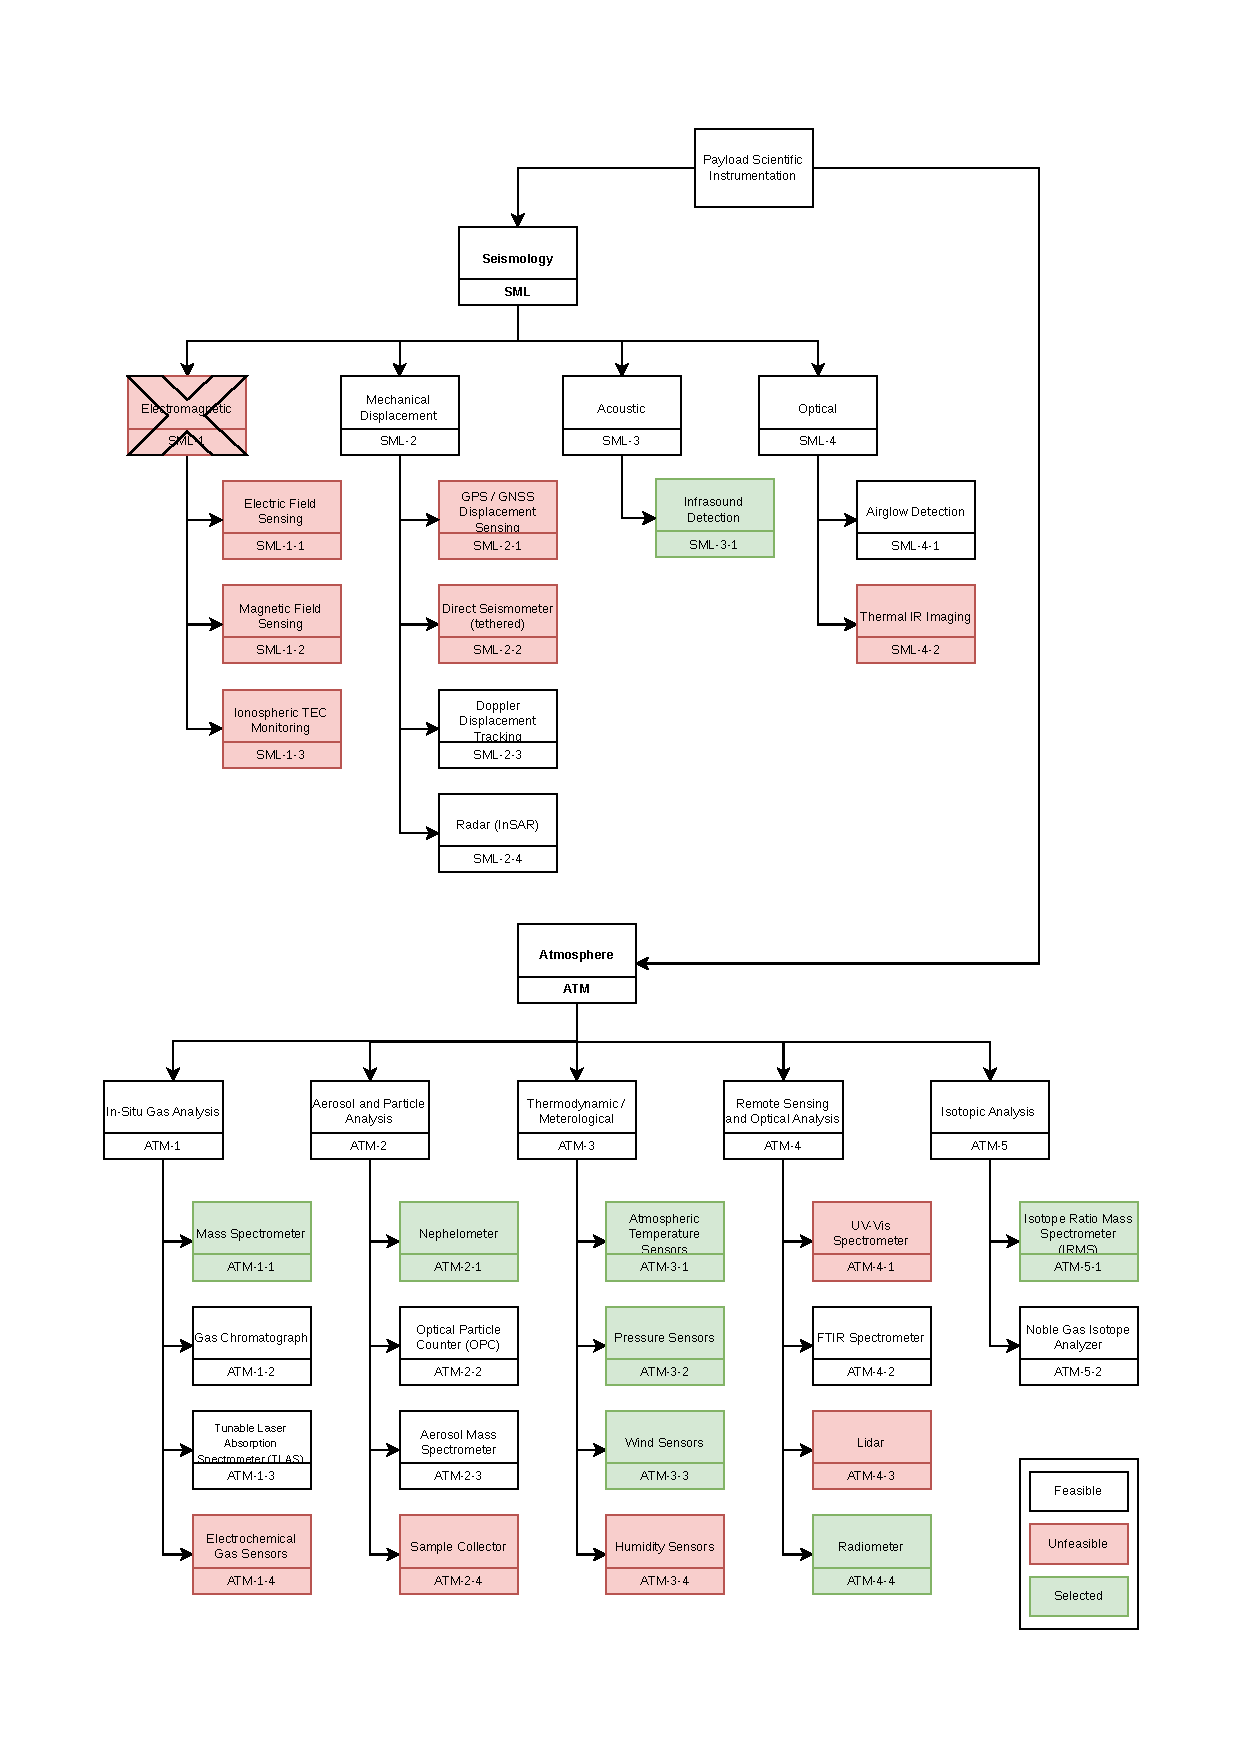
\includegraphics[
%             page=1,
%             width=\linewidth
%         ]{fig/WFD-DOT_payload.drawio22.pdf}
%     \end{minipage}
%     \vfill
%     \begin{minipage}{\textwidth}
%         \caption{Design Option Tree Payload Subsystem}
%         \label{fig:dot_payload}
%     \end{minipage}

% \end{figure}

\subsection{Seismic Measurement}

There are many ways to measure seismic activity from an aerial platform. In \autoref{fig:dot_payload}, a design option tree presents the options for seismology measurements from a balloon. The tree clarifies which options are feasible, unfeasible and the preferred selected options to be further considered on later design stages. The primary modes of measurement include electromagnetic analysis, mechanical displacement detection, acoustic analysis, and optical imaging. Each level has different measuring techniques that are presented as sub-levels in the tree. The rationale and explanation of each method is presented below. 

% The scientific objectives of this part of the VISTA mission and its connection to relevant requirements is presented in \autoref{tab:seismic_objectives}. 

% \begin{table}[H]
% \centering
% \small
% \caption{Seismic science objectives and their links to mission requirements and VEXAG Goals, Objectives, and Investigations.}
% \label{tab:seismic_objectives}

% \renewcommand{\arraystretch}{1.15}
% \setlength{\tabcolsep}{6pt}

% \begin{tabularx}{\textwidth}{|
% >{\raggedright\arraybackslash}X|
% >{\raggedright\arraybackslash}p{5.2cm}|}
% \hline
% \textbf{Science Objective} & \textbf{Relevance} \\
% \hline

% Detection and characterisation of Venusquakes and volcanic eruptions to determine whether Venus is presently seismically and volcanically active, and to constrain the frequency and magnitude distribution of seismic events. &
% VEXAG III.A.2 Geologic Activity; VEXAG I.A.1 Crustal Recycling; REQ-F-SCI-06 \\
% \hline

% Identification of dominant atmospheric gravity-wave source regions and assessment of whether these are topographically controlled, providing insight into surface--atmosphere mechanical coupling on Venus. &
% VEXAG II.A.2 Mesoscale Processes; VEXAG II.A.1 Deep Dynamics; VEXAG III.A.2 Geologic Activity; REQ-F-SCI-06 \\
% \hline

% \end{tabularx}
% \end{table}

For the first level, an option considered is using electromagnetic waves for the detection of seismic activity. A few options that make use of such method were explored, however they were all deemed unfeasible under Venus' conditions, therefore such method will be eliminated from the considered concepts. 

\begin{itemize}
    \item \textbf{SML-1-1}: This method requires measuring dc and very low frequency electric fields. Venus conditions can pose quite a challenge to this method. The high conductivity of the atmosphere due to the high temperatures makes the signals dissipate quickly and electrical circuits tend to short-circuit \cite{SML-1-1}. Moreover, the dense atmosphere and the thick cloud layer may also contribute to signal attenuation and noise production. These factors gravely impacts the ability of accurate measurements and seismic activity detection, therefore such method is considered unfeasible. 
    \item \textbf{SML-1-2}: Venus lacks an intrinsic magnetic field. There may be a very weak induced magnetic field created by the interaction between solar wind and Venus' ionosphere. However, such field is not strong enough for a clear distinguish between noise and electromagnetic waves to be made, therefore such method is also considered unfeasible. 
    \item \textbf{SML-1-3}: Such technique involves the measurement of the total electron content in the ionosphere, however it requires technology not yet present on Venus. This includes a GNSS (Global Navigational Satellite System), as well as extensive ground station coverage \cite{SML-1-3}. For the aforementioned reasons, this methods was also deemed unfeasible.      
\end{itemize}

Another option considered for determining seismic activity involves the measurement of surface displacement due to such geological events. Some techniques are also deemed unfeasible due to the lack of technology present in Venus. Other methods, although still feasible, may present some challenges given the mission conditions. Therefore, using mechanical displacement as primary measurement was discarded. 
\begin{itemize}
    \item \textbf{SML-2-1}: As mentioned previously, Venus does not possess a GNSS or global GPS system, therefore this technique is discarded from the option possibilities. 
    \item \textbf{SML-2-2}: A direct seismometer requires the instrument to be placed near or/and at the surface for accurate measurements to be made. Due to the high temperatures near the surface, no equipment would survive the required mission length. Moreover, a tether of over 50 km is also considered unfeasible for this mission due to its complex engineering implications. 
    \item \textbf{SML-2-3}: 
    \item \textbf{SML-2-4}: This system serves specifically well for ground and topography mapping, as the radio waves are capable of penetrating the cloud layer of Venus. However, such technology may present some limitations for an aerial balloon platform on Venus. In order to detect changes in altitude, repeat orbits are necessary in order to take measurements of the same location. As the balloon presents little to no control capability, and instead flows according to the planet's wind, ensuring repeat orbits is a challenge. 
\end{itemize}

A third category of measurement technique involves the study of the seismo-acoustic waves produced by seismic activity and that are later propagated through the atmosphere. This method shows to be the most promising for future Venus missions. 

\begin{itemize}
    \item \textbf{SML-3-1}: Due to Venus’s dense atmosphere, there is strong coupling between the solid surface and the atmosphere. As these waves travel upward, they preserve key characteristics of the original seismic surface waves, including their frequency content and dispersion. This makes it possible for a balloon platform to obtain accurate and reliable measurements by measuring pressure fluctuations in the atmosphere \cite{SML-3-2}. Therefore, this is a very strong contender for the detection of seismic activity within the possible options. 
\end{itemize}

The fourth, and last, measuring technique considered involves optical analysis of either the upper atmosphere layer of Venus, or the thermal imaging of the surface. 

\begin{itemize}
    \item \textbf{SML-4-1}: This technique presents limitations for an aerial balloon platform, as it requires higher observational altitudes and a larger imaging area of the planet. This approach is more effective when combined with an orbiter, which can provide a much wider field of view due to its higher altitude, enabling continuous monitoring over a defined region. A cooperative system could therefore be preferred, where the orbiter acts as a communication relay and provides global context, while the balloon functions as a local tracking station, offering higher-resolution measurements of atmospheric perturbations \cite{seism1}. Although limited, it still presents as an option for seismic detection.
    \item \textbf{SML-4-2}: As the temperature at the surface is extremely high, over \SI{450}{\celsius}, distinguishing small thermal anomalies provoked by seismic activity on the surface can become very challenging. Due to the high sensitivity to noise of this method, it was determined unfeasible for the mission.
\end{itemize}

Acoustic measurement via infrasound detection is the only feasible seismic sensing method for the VISTA balloon platform. Barometers measure atmospheric pressure fluctuations, which can be directly related to ground motion in the infrasound frequency range. A balloon drifting with the wind experiences reduced background wind noise compared to a fixed station, and atmospheric attenuation in Venus's ($CO_2$) atmosphere is negligible for wave periods above one second. Over the five-year mission duration, even a low seismic event rate of one event per year yields a high detection probability. Infrasound detection is therefore baselined as the primary seismic sensing mode, implemented through the barometer array described in the following sections. Optical instruments coupled with an orbiter remain a complementary option to be explored in later design stages, independent of the current payload subsystem.

% Source Twan:  https://www.sciencedirect.com/science/article/pii/S1270963821001176

% Based on the rationale for each instrumentation method, it can be concluded that only acoustic measurements and optical instruments coupled with an orbiter are feasible to produce the results required for the mission. Even for the remaining feasible options, the challenges that each component impose, makes them not suitable, and therefore, discarded options. 

% Infrasound wave detection presents many advantages when used in the Venus atmosphere compared to other methods. Infrasound detection is achieved by measuring pressure fluctuations in the atmosphere using barometers. In the infrasound frequency range, these pressure variations can be directly related to the underlying ground motion through a proportional relationship. The minimum number of seismic events per year required for wave detection decreases with increasing mission duration. In other words, the longer the mission duration, the greater the likelihood of detecting events, even if they occur infrequently. With the current mission concept lasting five years, and assuming an average of only one geological event per year, the balloon platform would likely already be capable of detecting such seismic signals.

% Regarding wave interference, a balloon drifting with the wind experiences lower background wind noise than a fixed ground station, since the relative wind velocity is reduced. Atmospheric attenuation can also dampen wave energy. In Venus’s atmosphere, this effect is mainly controlled by the relaxation of \(CO_2\) molecules, but it is only significant for acoustic waves with periods shorter than one second \cite{SML-3-2}. This effect will be discussed further in later stages of the design.

% As infrasound wave detection is the most promising approach for an aerial balloon platform within the presented options, this will be used as primary mode for the detection of seismic activity in the VISTA mission. That is, no trade-off will be made for the seismology instruments. Such detection is made through the use of barometers, that can be assembled in many ways. The option for the use of optical instruments may still be explored in later stages, depending on remaining mass and cost budget. However, as this instrument influences mainly the orbiter, such possibility can be considered independent of the current instrumental payload subsystem design. The different assembly design options of the payload subsystem will be presented later on once the instruments for the atmospheric measurement have been selected.


\subsection{Atmospheric Measurement}

The atmospheric science to be conducted on Venus is more extensive, and instruments' functions may overlap or be combined to suffice the same scientific objectives. \autoref{tab:science_objectives} presents the science objectives, with its corresponding relevance connection, and the possible candidate instruments present in the tree that can serve such purpose. 

The atmospheric science objectives of the VISTA mission span four broad themes. First, cloud chemistry and habitability: characterisation of H\textsubscript{2}SO\textsubscript{4} concentration, acidity, and water vapour content throughout the cloud deck — the two primary habitability indicators — alongside in-situ measurement of gas species and aerosol composition, size distribution, and altitudinal variation, addressing VEXAG II.B.1, II.B.2, and REQ-F-SCI-01. Second, atmospheric dynamics: measurement of the meridional circulation and Hadley cell structure, detection of thermal tides and planetary-scale waves, and characterisation of convective activity, gravity wave propagation, and turbulence within the cloud layer, addressing VEXAG II.A.1, II.A.2, and REQ-F-SCI-05/07/08. Third, super-rotation: constraining the interaction between mean flow, wave activity, and convective processes that collectively maintain Venus's retrograde zonal super-rotation, addressing VEXAG II.A.1/II.A.2 and REQ-F-SCI-07/08. Fourth, radiative balance: measurement of upwelling and downwelling radiative fluxes across multiple spectral bands to determine altitude-dependent energy deposition and its role in driving circulation, addressing VEXAG II.B.1 and REQ-F-SCI-10/11. Candidate instruments identified across these objectives include the Mass Spectrometer (ATM-1-1), Gas Chromatograph (ATM-1-2), TLAS (ATM-1-3), Nephelometer (ATM-2-1), Optical Particle Counter (ATM-2-2), Aerosol Mass Spectrometer (ATM-2-3), pH Sensor (ATM-2-5), Atmospheric Temperature Sensors (ATM-3-1), Pressure Sensors (ATM-3-2), Wind Sensors (ATM-3-3), Radiometer (ATM-4-4), and FTIR Spectrometer (ATM-4-2), complemented by balloon drift tracking for absolute wind velocity recovery.

% \begingroup
% \footnotesize
% \renewcommand{\arraystretch}{1.18}
% \setlength{\tabcolsep}{4pt}
% \setlength{\LTpre}{0.3em}
% \setlength{\LTpost}{0.6em}

% \begin{longtable}{@{}
% >{\raggedright\arraybackslash}p{0.41\textwidth}
% >{\raggedright\arraybackslash}p{0.22\textwidth}
% >{\raggedright\arraybackslash}p{0.30\textwidth}
% @{}}

% \caption{Atmospheric science objectives, their links to mission requirements and VEXAG Goals, Objectives, and Investigations, and the candidate instruments that address each objective.}
% \label{tab:science_objectives}\\

% \toprule
% \textbf{Science Objective} & \textbf{Relevance} & \textbf{Candidate Instruments} \\
% \midrule
% \endfirsthead

% \caption[]{Atmospheric science objectives, continued.}\\
% \toprule
% \textbf{Science Objective} & \textbf{Relevance} & \textbf{Candidate Instruments} \\
% \midrule
% \endhead

% \midrule
% \multicolumn{3}{r}{\footnotesize Continued on next page} \\
% \endfoot

% \bottomrule
% \endlastfoot

% Characterisation of H\textsubscript{2}SO\textsubscript{4} concentration and acidity levels throughout the cloud layer. &
% VEXAG II.B.1 Interactions; REQ-F-SCI-01 &
% ATM-2-5 pH Sensor; ATM-1-1 Mass Spectrometer (indirect, via SO\textsubscript{3}/H\textsubscript{4} detection); ATM-1-3 TLAS \\

% \addlinespace

% Measurement of water vapour content and droplet-phase water activity within the cloud deck, which together with acidity constitute the two primary habitability indicators of the Venusian atmosphere. &
% VEXAG II.B.1 Interactions; VEXAG I.A.2 Atmospheric Losses; REQ-F-SCI-01 &
% ATM-1-3 TLAS; ATM-1-1 Mass Spectrometer; ATM-2-5 pH Sensor; ATM-2-1 Nephelometer \\

% \addlinespace

% In-situ characterisation of atmospheric gas species and cloud aerosol particles, including their chemical composition, size distribution, and variation with altitude throughout the cloud column. &
% VEXAG II.B.2 Aerosols; VEXAG II.B.1 Atmospheric Chemistry; REQ-F-SCI-01 &
% ATM-1-1 Mass Spectrometer; ATM-1-2 Gas Chromatograph; ATM-1-3 TLAS; ATM-2-1 Nephelometer; ATM-2-2 Optical Particle Counter; ATM-2-3 Aerosol Mass Spectrometer; ATM-4-2 FTIR Spectrometer \\

% \addlinespace

% Measurement of the mean meridional circulation pattern, including equatorward wind velocities in the lower cloud levels and poleward winds at higher altitudes, to characterise the Hadley cell structure driving global atmospheric transport. &
% VEXAG II.A.1 Deep Dynamics; REQ-F-SCI-07; REQ-F-SCI-08 &
% ATM-3-3 Wind Sensors (primary); ATM-3-2 Pressure Sensors (altitude-resolved structure); ATM-3-1 Atmospheric Temperature Sensors; Balloon Drift Tracking \\

% \addlinespace

% Detection and characterisation of thermal tides and planetary-scale atmospheric waves. &
% VEXAG II.A.2 Mesoscale Processes; VEXAG II.A.1 Deep Dynamics; REQ-F-SCI-07 &
% ATM-3-2 Pressure Sensors; ATM-3-3 Wind Sensors; ATM-3-1 Atmospheric Temperature Sensors; ATM-4-4 Radiometer (radiative forcing of tides) \\

% \addlinespace

% In-situ measurement of convective activity, gravity wave generation and propagation, and turbulence within the cloud layer. &
% VEXAG II.A.2 Mesoscale Processes; REQ-F-SCI-05; REQ-F-SCI-07 &
% ATM-3-2 Pressure Sensors; ATM-3-3 Wind Sensors; ATM-3-1 Atmospheric Temperature Sensors; Balloon Drift Tracking (mesoscale displacement) \\

% \addlinespace

% Characterisation of mean flow, wave activity, and convective processes to constrain how these phenomena interact and collectively maintain the retrograde zonal super-rotation of the Venusian atmosphere. &
% VEXAG II.A.1 Deep Dynamics; VEXAG II.A.2 Mesoscale Processes; REQ-F-SCI-07; REQ-F-SCI-08 &
% ATM-3-3 Wind Sensors; ATM-3-2 Pressure Sensors; ATM-3-1 Atmospheric Temperature Sensors; ATM-4-4 Radiometer (radiative-dynamical coupling); Balloon Drift Tracking \\

% \addlinespace

% Measurement of both upwelling and downwelling radiative fluxes across multiple spectral bandpass channels throughout the cloud layer, to determine the altitude-dependent deposition of solar and thermal energy and its role in driving atmospheric circulation. &
% VEXAG II.B.1 Radiative Balance; REQ-F-SCI-10; REQ-F-SCI-11 &
% ATM-4-4 Radiometer; ATM-4-2 FTIR Spectrometer; ATM-3-1 Atmospheric Temperature Sensors \\

% \end{longtable}
% \endgroup
% 1,2 - important on cloud habitability 
% \begin{enumerate}
%     \item \textbf{Cloud acidity}: Characterisation of H\textsubscript{2}SO\textsubscript{4} concentration and acidity levels throughout the cloud layer.
    
%     \item \textbf{Water activity}: Measurement of water vapour content and droplet-phase water activity within the cloud deck, which together with acidity constitute the two primary habitability indicators of the Venusian atmosphere.

%     \item \textbf{Gas and aerosol composition}: In-situ characterisation of atmospheric gas species and cloud aerosol particles, including their chemical composition, size distribution, and variation with altitude throughout the cloud column.

%     \item \textbf{Large-scale circulation}: Measurement of the mean meridional circulation pattern, including equatorward wind velocities in the lower cloud levels and poleward winds at higher altitudes, to characterise the Hadley cell structure driving global atmospheric transport.

%     \item \textbf{Atmospheric waves}: Detection and characterisation of thermal tides and planetary-scale waves.

%     \item \textbf{Mesoscale dynamics}: In-situ measurement of convective activity, gravity wave generation and propagation, and turbulence within the cloud layer.

%     \item \textbf{Coupled dynamics}: Characterisation of mean flow, wave activity, and convective processes to constrain how these phenomena interact and collectively maintain the retrograde zonal super-rotation of the Venusian atmosphere.

%     \item \textbf{Radiative flux Variation}: Measurement of both upwelling and downwelling radiative fluxes across multiple spectral bandpass channels throughout the cloud layer, to determine the altitude-dependent deposition of solar and thermal energy and its role in driving atmospheric circulation.
% \end{enumerate}


% % \begin{enumerate}
% %     \item venus quakes / volcanic eruptions - if venus is seismically active 
% %     \item mean thickness of venus crust
% %     \item dominant source regions for gravity waves and if they are related to topography 

% % \end{enumerate}

Having such scientific goals as primary drive for selecting the instruments, the following options are discussed and determined whether or not those are to be included in the final VISTA mission configuration.   

\begin{itemize}
    \item \textbf{ATM-1-1}: Fundamental instrument for chemical composition determination. It is the highest-value single instrument for identifying bulk atmospheric constituents, trace gases, and isotopic ratios including D/H. Due to its high versatility and scientific output, it is crucial to include such instrument. 
    
    \item \textbf{ATM-1-2}: The gas chromatograph is capable of separating and identifying atmospheric gas species. However, it is functionally redundant with the mass spectrometer (ATM-1-1), which offers broader species coverage and higher sensitivity. Including both would increase mass and power consumption without proportional science return given the constraints of REQ-C-SUB-01 and REQ-C-SUB-06. Therefore, such instrument will not be included.
    
    \item \textbf{ATM-1-3}: The Tunable Laser Absorption Spectrometer provides high-sensitivity, species-specific detection of trace gases including SO\textsubscript{2}, HCl, and H\textsubscript{2}O that are of direct relevance to Venus cloud chemistry and VEXAG science goals (REQ-F-SCI-09). It complements the mass spectrometer by providing continuous in-situ trace gas monitoring at lower power than a standalone mass spectrometer sweep. Therefore, such instrument is included into the instrumentation payload. 
    
    \item \textbf{ATM-1-4}: Electrochemical gas sensors are destroyed by the concentrated sulfuric acid environment of the Venus cloud deck. This does not comply with REQ-F-ENV-03, which requires that the aerobot shall not degrade in Venus's toxic atmosphere. Therefore, this option is deemed unfeasible. 
\end{itemize}

\begin{itemize}
    \item \textbf{ATM-2-1}: The nephelometer directly characterizes aerosol and cloud particle properties through light scattering. It satisfies REQ-F-SCI-01 for aerosol sampling and cloud analysis, and it has been put to test in the Venus H\textsubscript{2}SO\textsubscript{4} cloud environment specifically. Due to its high TRL and science output, this instrument is included into the payload. 

    \item \textbf{ATM-2-2}: The Optical Particle Counter complements the nephelometer by providing particle size distribution data that the nephelometer alone cannot resolve. When coupled together, it is possible to provide a complete aerosol characterization: nephelometer outputs the bulk scattering properties while OPC gives the size spectrum. Low power consumption makes it compatible with REQ-C-SUB-06. Therefore such instrument is also added into the payload count list.

    \item \textbf{ATM-2-3}: The Aerosol Mass Spectrometer would provide direct chemical composition of individual aerosol particles, offering higher specificity than the nephelometer. However, it adds significant mass and complexity on top of the ATM-2-1 and ATM-2-2 combination, which already satisfies REQ-F-SCI-01. The marginal science gain does not justify the additional resource cost within the constraints of REQ-C-SUB-01 and REQ-C-PAY-02. Therefore, such instrument option is no longer considered. 

    \item \textbf{ATM-2-4}: The sample collector does not comply with two requirements at the same time. First, the H\textsubscript{2}SO\textsubscript{4} environment reacts with collection substrates, constituting degradation, which goes against REQ-F-ENV-03. Secondly, chemical interaction between the sulfuric acid aerosol and the substrate alters the sample composition before analysis, directly impacting REQ-F-SCI-02, which requires that the sampling system shall not affect the chemical composition of the sample. Therefore, this instrument is not considered further in the design options. 

    \item \textbf{ATM-2-5}: The pH sensor is crucial for the measure of the acidity levels on the Venus cloud layer. As it is light and consumes low power, such instrument is added into the instrumentation load. 
\end{itemize}

As for the thermodynamic and meteorological measurements of the VISTA mission, most instruments are fundamental for the mission's scientific objectives. Therefore, almost all options are included into the aerobot bus.

\begin{itemize}
    \item \textbf{ATM-3-1}: Atmospheric temperature sensors directly satisfy REQ-F-SCI-10 and are among the lowest-risk, lowest-mass instruments in the entire payload. Continuous temperature profiling is a fundamental atmospheric science measurement and a prerequisite for interpreting data from nearly all other instruments.

    \item \textbf{ATM-3-2}: Pressure sensors directly satisfy REQ-F-SCI-11 and serve a dual purpose: atmospheric science measurement and is the primary seismic detection instrument (infrasound coupling), making it a fundamental instrument of the payload subsystem.

    \item \textbf{ATM-3-3}: Wind sensors directly satisfy REQ-F-SCI-05 and REQ-F-SCI-07 for cloud dynamics and vertical wind speed measurement. This instrument is crucial for characterising atmospheric turbulence structure, and convective dynamics within the Venusian cloud layer. As the balloon floats with the wind, horizontal wind speed measurement will be performed via tracking of the balloon's position, which will be done by GNC.  

    \item \textbf{ATM-3-4}: Standard humidity and water vapour sensors rely on materials and operating principles that are incompatible with the concentrated sulfuric acid environment at the Venus cloud deck, directly violating REQ-F-ENV-03. Dedicated H\textsubscript{2}O detection is instead addressed through the TLAS (ATM-1-3), which can measure water vapour spectroscopically without exposing sensitive materials to the atmosphere. Therefore, this instrument is not considered further in the design options.
\end{itemize}

As for remote sensing and optical analysis of the atmosphere, most instruments are deemed unfeasible. However, the inclusion of radiometers is still deemed of high importance for the mission. 

\begin{itemize}
    \item \textbf{ATM-4-1}: Although a UV-Vis spectrometer is physically survivable at the Venusian cloud deck altitude, the optically thick cloud deck severely limits nadir viewing depth, preventing meaningful surface or lower atmosphere measurements. The resulting science return does not justify the mass and power allocation, and the instrument does not directly satisfy any stated system requirement. Therefore, this instrument is not considered further in the design options.

    \item \textbf{ATM-4-2}: A FTIR spectrometer is physically viable at the balloon operating altitude and could provide broad-spectrum atmospheric composition data. However, the dense CO\textsubscript{2} atmosphere saturates many key infrared absorption bands, significantly limiting its effective species coverage. The science return that remains accessible is largely covered by the TLAS (ATM-1-3) at lower mass and power, making the FTIR redundant within the resource constraints of REQ-C-SUB-06.

    \item \textbf{ATM-4-3}: LIDAR does not fit within the mission requirements. As this system has a very high power consumption, not surpassing the power limit among all subsystems when using LIDAR is potentially not feasible, deeming this method not an option for the instruments list.

    \item \textbf{ATM-4-4}: The radiometer measures net longwave IR radiative flux across the cloud deck. Operating one unit nadir-facing and one zenith-facing provides the net radiative balance at cloud altitude, a fundamental input to Venus atmospheric models and a VEXAG roadmap goal (REQ-F-SCI-09). 
\end{itemize}

Finally, the isotopic analysis of the atmosphere. Such options were not selected at the end, as some instruments can be combined with other instruments already selected for the mission. 

\begin{itemize}
    \item \textbf{ATM-5-1}: The Isotope Ratio Mass Spectrometer is one of the highest science-value instruments for any Venus atmospheric mission. Hardware overlap with ATM-1-1 is possible, potentially allowing a combined mass spectrometer and IRMS implementation that reduces the total mass and power impact.

    \item \textbf{ATM-5-2}: The Noble Gas Isotope Analyzer functionality overlaps substantially with the mass spectrometer and IRMS. Therefore, this option is not considered. 
\end{itemize}

Based on the discussed rationales, the final selected instruments are coloured in green in the design option tree. In the following section, an estimate of the instruments specs for the sizing of this and other subsystems is provided. 

\begin{figure}[H]
    \centering

    \begin{minipage}{0.6\textwidth}
        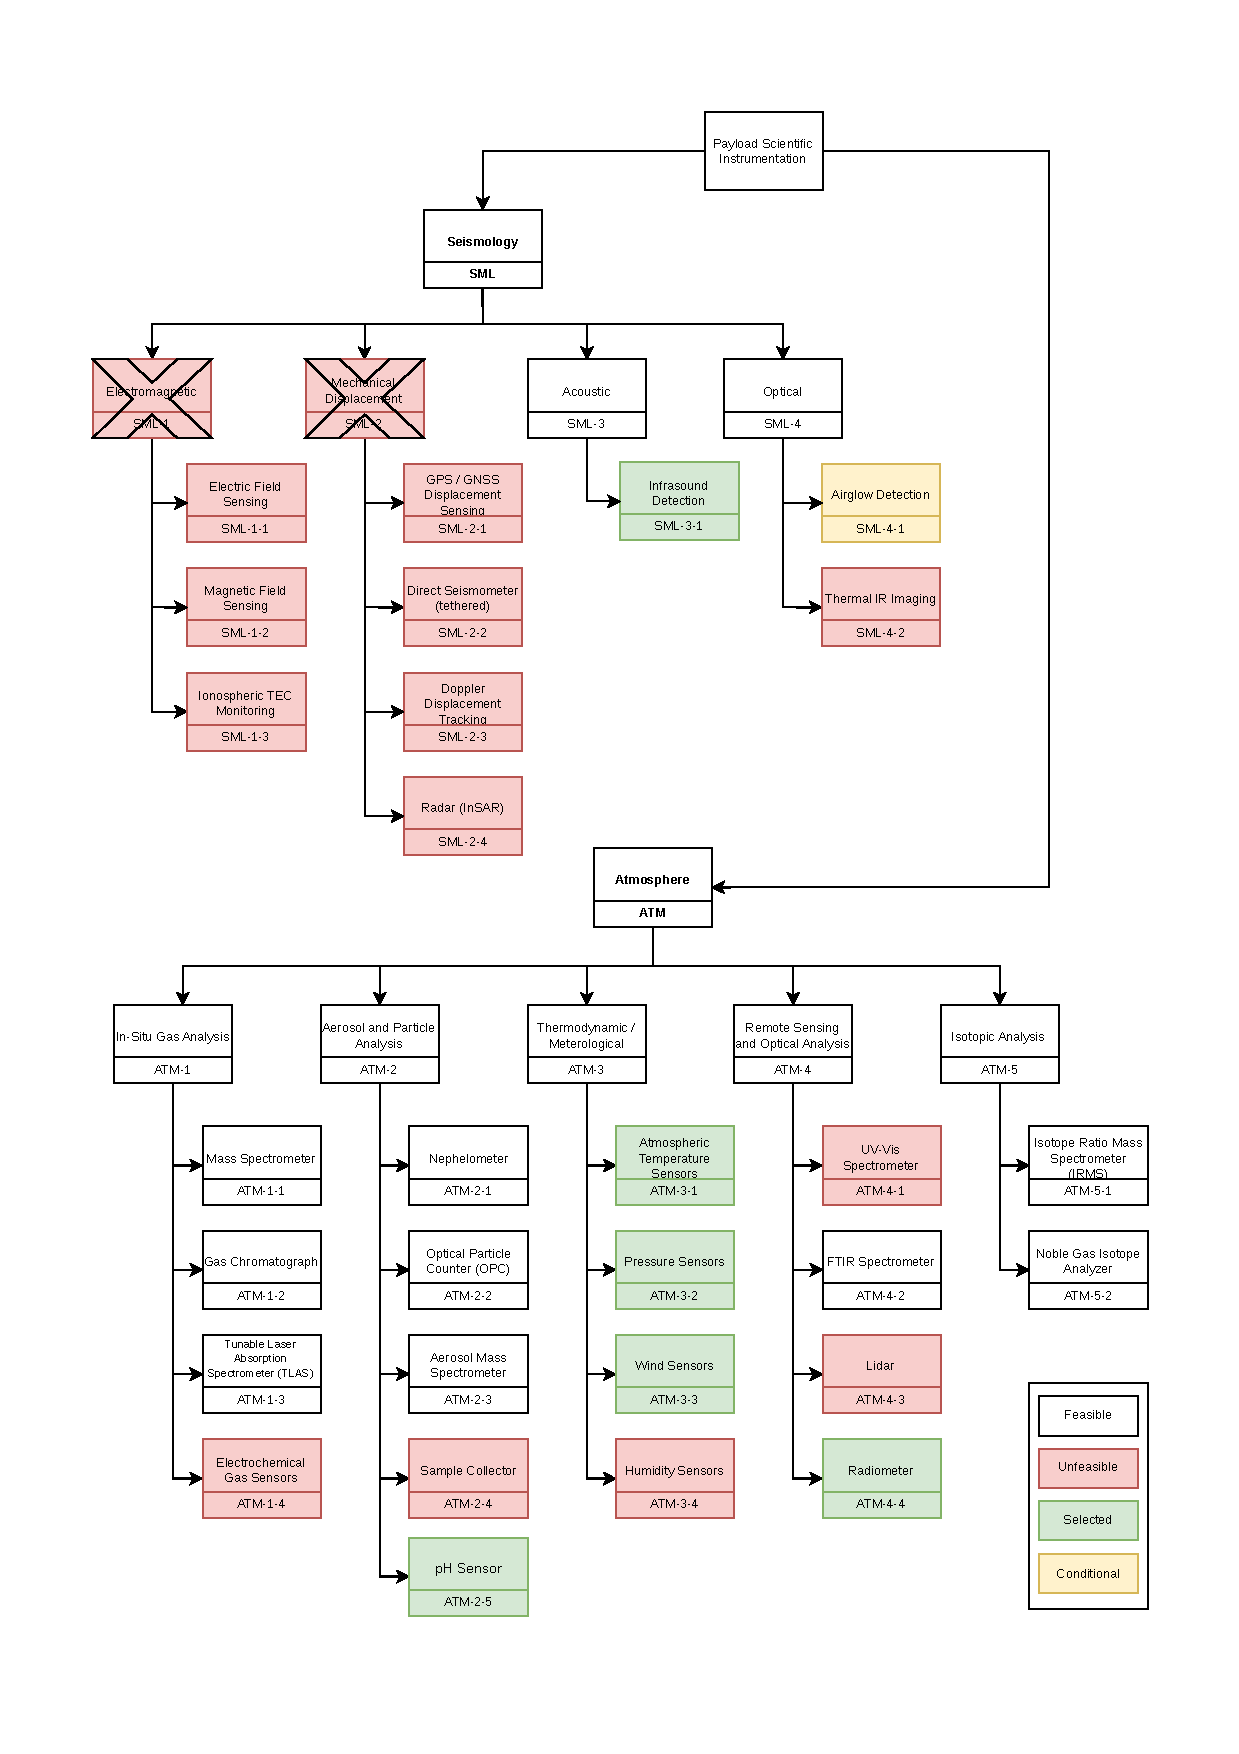
\includegraphics[
            page=1,
            width=\linewidth
        ]{fig/WFD-DOT_payload.drawio (2).pdf}
    \end{minipage}
    \vfill
    \begin{minipage}{\textwidth}
        \caption{Design Option Tree Payload Subsystem}
        \label{fig:dot_payload}
    \end{minipage}

\end{figure}


% \section{Instruments Trade-off}
% \label{sec:tradeoff_payload}
% Now that all instrument options have been presented, a trade-off to select the best techniques must be performed. The methods deemed infeasible in the previous section will not be considered in the trade-off. Due to the fact that some instruments are non-negotiable for satisfying the scientific requirements, they are automatically considered as part of the payload. Such instruments include: temperature sensors, pressure sensors, and wind sensors. The remaining 10 options fit different study categories and, although presented in the same table, are traded for different measurement purposes. There are four main groups of instruments that must be traded-off. The first refers to the atmospheric composition determination. Both a mass spectrometer and gas chromatography are able to accomplish the job, therefore a choice must be made. The second group refers to trace gas detection, where different techniques can be used to accomplish the similar results. The third ensures aerosol and particle characterisation, therefore a trade-off between nephelometer, an OPC and aerosol mass spectrometer must be performed. Finally, the fourth group refers to the isotopic analysis of the atmosphere. A choice must be made between using an IRMS or a noble gas isotope analyzer. 

% Different criterion for the trade-off have been established. That includes: scientific return of instrument, the corresponding TRL, mass, power consumption, reliability, and accuracy. Different weights are given to each criteria. The definition and scoring basis for each criterion is explained in \autoref{tab:tradeoff-criteria-payload}. The final atmospheric instruments trade-off table is presented in \autoref{trade-off-payload}. The different trade groups (1 through 4), as described above, are enumerated on the left side of the table for later reference. 

% % \begin{table}[H]
% % \centering
% % \caption{Trade-off criteria, definitions, and weights for balloon envelope material selection.}
% % \label{tab:tradeoff-criteria}
% % \footnotesize
% % \renewcommand{\arraystretch}{1.15}
% % \setlength{\tabcolsep}{4pt}
% % \begin{tabularx}{\linewidth}{@{}p{0.4cm} p{3.4cm} X p{1.0cm}@{}}
% % \toprule
% % \textbf{\#} & \textbf{Criterion} & \textbf{Definition and scoring basis} & \textbf{Weight} \\
% % \midrule
% % 1 & Scientific Return & Some instruments have higher scientific return than others and can provide multiple conclusions with fewer instrument combinations. This evaluates the amount of   & 30\% \\
% % 2 & TRL and flight heritage & TRL above 4 is a mission requirement, and the higher the TRL the better, therefore this is important criteria & 20 \% \\
% % 3 & Mass & Lower the mass the better, so important & 10\% \\
% % 4 & Power Consumption &  & 20\% \\
% % 5 & Reliability &  & 10\% \\
% % 6 & Accuracy &  & 10\% \\
% % \midrule
% % \multicolumn{3}{l}{\textit{Total}} & \textbf{100\%} \\
% % \bottomrule
% % \end{tabularx}
% % \end{table}


% \begin{table}[H]
% \centering
% \caption{Trade-off criteria, definitions, and weights for instrument selection.}
% \label{tab:tradeoff-criteria-payload}
% \footnotesize
% \renewcommand{\arraystretch}{1.15}
% \setlength{\tabcolsep}{4pt}
% \begin{tabularx}{\linewidth}{@{}p{0.4cm} p{3.4cm} X p{1.0cm}@{}}
% \toprule
% \textbf{\#} & \textbf{Criterion} & \textbf{Definition and scoring basis} & \textbf{Weight} \\
% \midrule

% 1 & Scientific Return &
% How directly and completely the instrument addresses the stated science objectives and VEXAG investigations, per REQ-STK-1.2. Score 1 (no direct link to any science objective) to 5 (crucial for VEXAG investigation and requirement compliance; removing it leaves a science objective entirely unaddressed).
% & 30\% \\
% \midrule

% 2 & TRL and Flight Heritage &
% Maturity of the instrument in Venus-relevant conditions. REQ-C-MIS-05 sets a hard minimum of TRL~4; instruments below this are non-compliant. Score 1 (TRL below 4) to 5 (TRL 8 and above, flight-demonstrated in Venus or directly analogous environment).
% & 20\% \\
% \midrule

% 3 & Mass &
% Instrument mass relative to the gondola cap of 200~kg (REQ-C-SUB-01). Score 1 (above 30~kg; incompatible with budget) to 5 (below 1~kg; negligible impact).
% & 10\% \\
% \midrule

% 4 & Power Consumption &
% Continuous power draw relative to the 500~Wh total energy storage cap shared across all subsystems (REQ-C-SUB-06). Weighted equally to TRL as it is the most crucial resource constraint. Score 1 (above 30~W; infeasible within budget) to 5 (below 1~W; negligible impact).
% & 20\% \\
% \midrule

% 5 & Reliability &
% Probability of sustained operation over the 5-year mission in the Venus H\textsubscript{2}SO\textsubscript{4} cloud environment, anchored to REQ-C-MIS-03 ($>$90\% survival) and REQ-C-PAY-01 ($>$80\% analysis success). Score 1 (likely to fail due to corrosion or mechanical wear within mission duration) to 5 (fully solid-state, no moving parts, no known H\textsubscript{2}SO\textsubscript{4} vulnerability).
% & 10\% \\
% \midrule

% 6 & Accuracy &
% Whether instrument precision meets the resolution required by the linked science objective under nominal Venus cloud deck operating conditions. Score 1 (precision insufficient to address the objective at any useful level) to 5 (precision exceeds the required resolution with comfortable margin under all expected conditions).
% & 10\% \\
% \midrule

% \multicolumn{3}{l}{\textit{Total}} & \textbf{100\%} \\
% \bottomrule
% \end{tabularx}
% \end{table}

% If any instruments present a scoring of 1 in any of the criterion, they are immediately discarded from the possible instrument options, as that means non compliance to the requirements. 

% \definecolor{score5}{RGB}{0,176,80}
% \definecolor{score4}{RGB}{146,208,80}
% \definecolor{score3}{RGB}{255,255,0}
% \definecolor{score2}{RGB}{255,192,0}
% \definecolor{score1}{RGB}{255,0,0}

% \begin{landscape}

% \scriptsize
% \renewcommand{\arraystretch}{1.35}
% \setlength{\tabcolsep}{2pt}

% \begin{longtable}{|
% >{\raggedright\arraybackslash}p{0.125cm}|
% >{\raggedright\arraybackslash}p{3.2cm}|
% >{\raggedright\arraybackslash}p{4.2cm}|
% >{\raggedright\arraybackslash}p{3.5cm}|
% >{\raggedright\arraybackslash}p{3cm}|
% >{\raggedright\arraybackslash}p{3.5cm}|
% >{\raggedright\arraybackslash}p{3cm}|
% >{\raggedright\arraybackslash}p{3.1cm}|
% >{\centering\arraybackslash}p{0.6cm}|}

% \caption{Instrument trade-off table}\\

% \hline
%  &
% \diagbox{\textbf{Instrument}}{\textbf{Criteria}}
% &
% \textbf{Scientific Return (30\%)}
% &
% \textbf{TRL (20\%)}
% &
% \textbf{Mass (10\%)}
% &
% \textbf{Power Consumption (20\%)}
% &
% \textbf{Reliability (10\%)}
% &
% \textbf{Accuracy (10\%)}
% &
% \textbf{Score}
% \\
% \hline
% \endfirsthead

% \hline
%  &
% \diagbox{\textbf{Instrument}}{\textbf{Criteria}}
% &
% \textbf{Scientific Return (30\%)}
% &
% \textbf{TRL (20\%)}
% &
% \textbf{Mass (10\%)}
% &
% \textbf{Power Consumption (20\%)}
% &
% \textbf{Reliability (10\%)}
% &
% \textbf{Accuracy (10\%)}
% &
% \textbf{Score}
% \\
% \hline
% \endhead

% % ---------------- MASS SPECTROMETER ----------------
% 1 &
% \textbf{Mass Spectrometer}
% & \cellcolor{score5!40}\textbf{5} Primary instrument for chemical composition and isotopic ratios
% & \cellcolor{score5!40}\textbf{5} Used previously in Venus and other space missions
% & \cellcolor{score2!40}\textbf{2} Among heavier instruments in the payload.
% & \cellcolor{score3!40}\textbf{3} Moderate power demand during active sampling.
% & \cellcolor{score5!40}\textbf{5} Flight-proven in Venus atmosphere.
% & \cellcolor{score5!40}\textbf{5} Very accurate chemical detection. 
% & \textbf{4.3}
% \\ \hline

% % ---------------- GC ----------------
% & 
% \textbf{Gas Chromatograph \cite{gas_chromo}}
% & \cellcolor{score3!40}\textbf{3} Limited identification capability.
% & \cellcolor{score5!40}\textbf{5} High TRL, tested previously in Venus missions.
% & \cellcolor{score2!40}\textbf{2} Among heavier instruments in the payload.
% & \cellcolor{score2!40}\textbf{2} High average power consumption.
% & \cellcolor{score4!40}\textbf{4} Heritage proven on previous missions.
% & \cellcolor{score4!40}\textbf{4} High resolution specs.
% & \textbf{3.0}
% \\ \hline


% % ---------------- IRMS ----------------
%  &
% \textbf{IRMS}
% & \cellcolor{score4!40}\textbf{4} Excellent for isotope analysis, but limited investigation scope.
% & \cellcolor{score3!40}\textbf{3} Venus-adapted IRMS not flight-demonstrated, development required.
% & \cellcolor{score2!40}\textbf{2} High mass.
% & \cellcolor{score3!40}\textbf{3} Moderate power, shares some hardware with mass spectrometer.
% & \cellcolor{score3!40}\textbf{3} Reduced reliability from history development gap.
% & \cellcolor{score5!40}\textbf{5} Extremely precise instrument.
% & \textbf{3.3}
% \\ \hline

% % ---------------- NOBLE GAS ----------------
% &
% \textbf{Noble Gas Isotope Analyzer}
% & \cellcolor{score3!40}\textbf{2} Limited identification capability.
% & \cellcolor{score3!40}\textbf{3} No Venus flight study, requires dedicated development.
% & \cellcolor{score2!40}\textbf{2} High mass, standalone instrument not shareable with mass spectrometer.
% & \cellcolor{score3!40}\textbf{3} Moderate power demand.
% & \cellcolor{score3!40}\textbf{3} Same development reliability concerns as IRMS.
% & \cellcolor{score2!40}\textbf{2} 
% & \textbf{2.8}
% \\ \hline

% \midrule

% % ---------------- TLAS ----------------
% 2 &
% \textbf{TLAS}
% & \cellcolor{score4!40}\textbf{4} High-sensitivity trace gas detection of SO\textsubscript{2}, HCl, H\textsubscript{2}O.
% & \cellcolor{score4!40}\textbf{4} High TRL but no Venus flight heritage.
% & \cellcolor{score4!40}\textbf{4} Compact solid-state design, lighter than other gas instruments.
% & \cellcolor{score4!40}\textbf{4} Low continuous power drawn.
% & \cellcolor{score4!40}\textbf{4} No moving parts, robust to vibration.
% & \cellcolor{score4!40}\textbf{4} Precision instrument for known gases 
% & \textbf{4}
% \\ \hline


% % ---------------- FTIR ----------------
% &
% \textbf{FTIR Spectrometer}
% & \cellcolor{score2!40}\textbf{2} Dense CO\textsubscript{2} saturates key IR bands.
% & \cellcolor{score4!40}\textbf{4} Mature technology but no Venus balloon study.
% & \cellcolor{score2!40}\textbf{2} Relatively heavy optical bench required.
% & \cellcolor{score3!40}\textbf{3} Moderate power, requires detector cooling.
% & \cellcolor{score3!40}\textbf{3} Interferometer moving mirror sensitive to vibration.
% & \cellcolor{score2!40}\textbf{2}Accurate but Venus conditions reduce effective retrieval quality.
% & \textbf{2.7}
% \\ \hline

% \midrule

% % ---------------- NEPHELOMETER ----------------
% 3 &
% \textbf{Nephelometer}
% & \cellcolor{score4!40}\textbf{4} Directly characterizes H\textsubscript{2}SO\textsubscript{4} cloud aerosol.
% & \cellcolor{score5!40}\textbf{5} Pioneer Venus heritage in identical environment.
% & \cellcolor{score4!40}\textbf{4} Lightweight optical instrument.
% & \cellcolor{score4!40}\textbf{4} Low power, passive scattering measurement.
% & \cellcolor{score5!40}\textbf{5} Extremely reliable, proven in Venus H\textsubscript{2}SO\textsubscript{4} clouds.
% & \cellcolor{score4!40}\textbf{4} Indirect inference of aerosol properties.
% & \textbf{4.3}
% \\ \hline

% % ---------------- OPC ----------------
% &
% \textbf{Optical Particle Counter (OPC)}
% & \cellcolor{score3!40}\textbf{3} Provides particle size distribution complementing nephelometer, not standalone.
% & \cellcolor{score4!40}\textbf{4} High TRL, however no Venus-specific testing.
% & \cellcolor{score5!40}\textbf{5} Very low mass.
% & \cellcolor{score5!40}\textbf{5} Negligible power consumption.
% & \cellcolor{score4!40}\textbf{4} Simple and robust optical design.
% & \cellcolor{score4!40}\textbf{4} 
% & \textbf{4.1}
% \\ \hline

% % ---------------- AEROSOL MS ----------------
% &
% \textbf{Aerosol Mass Spectrometer}
% & \cellcolor{score4!40}\textbf{4} Provides particle-level chemical composition beyond nephelometer capability.
% & \cellcolor{score3!40}\textbf{3} No Venus-specific heritage, adaptation required.
% & \cellcolor{score2!40}\textbf{2} Heaviest aerosol instrument option.
% & \cellcolor{score1!40}\textbf{1} High power demand limits compatibility with REQ-C-SUB-06.
% & \cellcolor{score2!40}\textbf{2} Reduced reliability from higher complexity and lack of testing in Venusian environment.
% & \cellcolor{score5!40}\textbf{5} Very accurate system.
% & \textbf{2.4}
% \\ \hline

% \midrule



% % % ---------------- RADIOMETER ----------------
% % \textbf{Radiometer}
% % & \cellcolor{score3!40}\textbf{3} Measures net IR radiative flux across cloud deck
% % & \cellcolor{score5!40}\textbf{5} Maximum maturity
% % & \cellcolor{score4!40}\textbf{4} Lightweight thermopile detectors.
% % & \cellcolor{score5!40}\textbf{5} Fully passive measurement, negligible power.
% % & \cellcolor{score5!40}\textbf{5} No moving parts, no environmental vulnerability.
% % & \cellcolor{score5!40}\textbf{5} Very simple, dual-unit nadir/zenith setup requires no active control.
% % & \textbf{4.4}
% % \\ \hline


% \end{longtable}

% \end{landscape}

\definecolor{score5}{RGB}{0,176,80}
\definecolor{score4}{RGB}{146,208,80}
\definecolor{score3}{RGB}{255,255,0}
\definecolor{score2}{RGB}{255,192,0}
\definecolor{score1}{RGB}{255,0,0}





\section{Instrument Selection}
\label{sec:instrument_selection}
% \autoref{tab:instruments} presents off the shelf models or estimate models from previous mission, in order to make a first estimation of the main budgets needed for the sizing of this as well as other subsystems. This includes the mass, power, and data rate budget, as well as, service temperature of each instrument, and corresponding volume. Nonetheless, most instruments will need modifications prior to the mission. 

% \begin{longtable}{%
%     p{3cm} |
%     p{2cm}
%     p{2cm}
%     p{2cm}
%     p{3cm}
%     p{2cm}
% }
% \caption{Payload Instrument Suite for a Venus 55~km Long-Duration Balloon Mission}
% \label{tab:venus_payload}\\
% \toprule
% \textbf{Instrument} &
% \textbf{Mass (kg)} &
% \textbf{Data Rate (kB/s)} &
% \textbf{Power (W)} &
% \textbf{Service Temperature\ ($^\circ$C)} &
% \textbf{Volume (cm$^3$)} \\
% \midrule
% \endfirsthead
% \toprule
% \textbf{Instrument} &
% \textbf{Mass (kg)} &
% \textbf{Data Rate (kB/s)} &
% \textbf{Power (W)} &
% \textbf{Service Temperature\ ($^\circ$C)} &
% \textbf{Volume (cm$^3$)} \\
% \midrule
% \endhead
% Neutral Mass Spectrometer (NMS) \cite{NMS} &
% 10.9 &
%  &
% 14 &
% $-20$ to $+50$ &
% 10650 \\
% \hline
% Auto-fluorescing Nephelometer (AFN) \cite{instruments} &
% 0.8 &
%  &
% 40 &
% $-10$ to $+40$ &
% 100 \\
% \hline
% % Particle Size Counter &
% % 0.45 &
% % 1 &
% % 1.5 &
% % $0$ to $+50$ &
% % --- \\
% \hline
% Weather Instrument Suite (WIS) \cite{instruments} &
% 0.1 &
% 0.05 &
% 1 &
% $-40$ to $+60$ &
% 98 \\
% \hline
% Sonic Anemometer \cite{Cheng2024StratosphericSonicAnemometer} &
% 3 &
%  &
% 5.3 &
% $-40$ to $+50$ &

% \\
% \hline
% Pressure Sensor (Barometer x5) \cite{barometers} & 0.450 & & 0.1 & -54 to +70 & 15.5
% \\
% \hline
% Mini Tunable Laser Spectrometer (mTLS) \cite{instruments} &
% 0.62 &
% 0.3  &
% 14 &
% $-40$ to $+80$ &
% 240 \\
% \hline
% Pyrgeometer \cite{pyro_radiometer} &
% 0.65 &
% 2.4 &
% 3 &
% $-40$ to $+80$ &
% 3530 \\
% \hline
% Tartu Observatory pH Sensor (TOPS) \cite{instruments} &
% 0.35 &
%  &
% 2 &
% $-20$ to $+50$ &
% 800 \\
% \bottomrule
% \end{longtable}

%bit rates are for telemtry, not necessarily raw data
%WIS data rate ranges from 7-400 bits/s depending on sampling. u can also do high sampling and then average with compression. This value is now for 1 every 10s 
%100 b/s to 3000 b/s based on sampling rate. for 2 Hz approximately 300 b/s
%mtls once every 4 hours
%tops 1 measurement every 10 seconds while it is on

%valus for NMS, AFN, mTLS, WIS, TOPS are sure
\begin{minipage}[t]{0.42\textwidth}
\small
\autoref{tab:instruments} presents off-the-shelf models or estimated models from previous missions in order to make a first estimation of the main budgets needed for the sizing of this and other subsystems. This includes the mass, power, data-rate budget, service temperature of each instrument, and corresponding volume. Nonetheless, most instruments will require modifications prior to the mission.
\end{minipage}
\hfill
\begin{minipage}[t]{0.54\textwidth}

\begin{table}[H]
\centering
\small
\setlength{\tabcolsep}{3pt}
\renewcommand{\arraystretch}{0.9}

\caption{Payload Instrument Suite for VISTA Mission}
\label{tab:venus_payload}

\begin{tabular}{lccccc}
\toprule
Instrument & 
Mass & 
Data & 
Power & 
Temp. & 
Vol. \\
& (kg) & (b/s) & (W) & ($^\circ$C) & (cm$^3$) \\
\midrule
NMS \cite{NMS} &
10.9 & 40\cite{hoffman1979pioneer} & 14 & -20 to 50 & 10650 \\
AFN \cite{instruments} &
0.8 & 1000\cite{baumgardner2022deducing} & 40 & -10 to 40 & 100 \\
WIS \cite{instruments} &
0.1 & 100 & 1 & -40 to 60 & 98 \\
Sonic Anemometer \cite{Cheng2024StratosphericSonicAnemometer} &
0.4 & 300 & 2 & -40 to 50 & 8000 \\
Barometers $\times5$ \cite{barometers} &
0.45 & 60 & 0.1 & -54 to 70 & 15.5 \\
mTLS \cite{instruments} &
0.62 & 500 & 14 & -40 to 80 & 240 \\
Pyrgeometer $\times2$ \cite{pyro_radiometer} &
0.65 & 300 & 3 & -40 to 80 & 3530 \\
TOPS \cite{instruments} &
0.35 & 800 & 2 & -20 to 50 & 800 \\
OPC \cite{OPC} & 
2 & 500 & 15 & -50 to 50 & 4500 \\
\bottomrule
\end{tabular}

\label{tab:instruments}
\end{table}

\end{minipage}
% ADD DUTY CYCLES, INTERVAL OF DATA GENERATION

\normalsize
\section{Sub-system Architectural Concepts}

Based on the instruments selected on the previous sections, different configuration arrangements can be considered for the gondola of the aerobot. Most instruments will be stored inside the gondola, where an inlet hole will connect them to the atmosphere when necessary. The pyrgeometers are required to be installed in a boom at a small distance from the gondola (around 10 cm). Moreover, the sonic anemometers also have part of its system sticking outside of the gondola, in order to determine the 3D vector of the wind. Therefore, the final 



\subsubsection*{Architecture A - Gondola Only}
All instruments are placed within the gondola, which is suspended beneath the balloon envelope. The gondola provides a controlled thermal and pressure environment, protecting sensitive electronics from the harsh Venusian atmosphere. Seismic detection will rely only in the barometers present within the gondola. While scientifically valid, this approach provides only indirect seismic sensing with limited localisation capability, and signal interpretation requires careful deconvolution from atmospheric noise. This architecture offers the highest instrument integration simplicity, lowest mechanical risk, and greatest thermal and pressure stability, making it the most robust baseline design.

\subsubsection*{Architecture B - Tethered Instruments}
Barometers are deployed along a tether hanging below the gondola, at varying lengths (15–300 m). By distributing pressure-sensing along the tether array, the system forms a vertical aperture that enables directional filtering of incoming acoustic-gravity wave signals. Cross-correlation of arrival-time differences between sensors at different altitudes allows triangulation of the wavefront bearing and, in combination with atmospheric propagation modelling, estimation of the seismic epicentre location. This significantly improves upon Architecture A's localisation capability. The tether design must account for Venusian wind shear at the cloud deck altitude, requiring careful dynamic analysis to avoid entanglement or resonance-driven oscillation. The tether and its sensor payload introduce additional mass and a deployment mechanism, raising complexity compared to Architecture A, but remain within heritage bounds of balloon tether systems tested in terrestrial stratospheric campaigns. This architecture represents a strong trade between enhanced science return and moderate additional mechanical risk. 

\subsubsection*{Architecture C - Towbody Probe}
A streamlined aeroshell probe, the towbody, is suspended on a long tether (1–60 km) below the balloon, descending beneath the Venusian cloud deck (\~48 km altitude) into the middle and lower atmosphere. The probe carries a dedicated instrument suite. Because the probe operates at higher pressures and temperatures than the balloon float altitude, it requires independent thermal protection and pressure vessel design, substantially increasing development complexity. The tether must sustain significant aerodynamic drag loads from differential winds between the float and probe altitudes, demanding careful materials selection and tether dynamics analysis. A separate power generating unit must also be considered. This architecture offers the most scientifically ambitious capability, with direct in-situ sub-cloud measurements as well as more seismic sensitivity due to closer proximity to the surface. However, it carries the highest mass, mechanical, and thermal risk of the three architectures, and the long tether introduces potential balloon stability perturbations that must be assessed through coupled flight dynamics modeling. 

\section{Subsystem architecture Trade-Off}
\label{sec:payload_tradeoff}
Given the three architectures presented in the previous section, a trade-off must now be performed in order to choose the selected instrument's payload final architecture. Five criteria were chosen with a corresponding attributed weight. The criteria with highest weight are related to their scientific value to the mission: Science Return (25\%) and Seismic Localisation (30\%). The remaining criteria are: Mission Risk (15\%), Mass \& Complexity (15\%), and Heritage \& Feasibility (15\%). They all carry equal weight, as they have shared importance as mission-enabling constraints. Finally, a score system is used in order to compute the best architecture. The scoring works as follows: \textbf{1} = severe deficiency, unfeasible; \textbf{2} = partial deficiency; \textbf{3} = meets requirement; \textbf{4} = exceeds requirement; \textbf{5} = significantly exceeds requirement. If any architecture presents score 1 in any criteria, they will be immediately discarded, despite the remaining scores in the other criteria. 



% Softer pastel palette
\definecolor{score1}{RGB}{242,180,180}   % pastel red
\definecolor{score2}{RGB}{245,205,160}   % pastel orange
\definecolor{score3}{RGB}{250,235,170}   % pastel yellow
\definecolor{score4}{RGB}{210,235,200}   % pastel green
\definecolor{score5}{RGB}{170,220,170}   % stronger pastel green

% All text black
\newcommand{\sone}[1]{\cellcolor{score1}\color{black}#1}
\newcommand{\stwo}[1]{\cellcolor{score2}\color{black}#1}
\newcommand{\sthree}[1]{\cellcolor{score3}\color{black}#1}
\newcommand{\sfour}[1]{\cellcolor{score4}\color{black}#1}
\newcommand{\sfive}[1]{\cellcolor{score5}\color{black}#1}

\begin{table}[htbp]
\centering
\caption{Instrument subsystem architecture trade-off}
\label{tab:arch_tradeoff}

% Smaller + tighter
\scriptsize
\renewcommand{\arraystretch}{1.15}
\setlength{\tabcolsep}{3pt}

\begin{tabular}{
  p{1.3cm}
  p{2.8cm}
  p{2.4cm}
  p{3.0cm}
  p{2.3cm}
  p{2.3cm}
  p{0.8cm}
}
\toprule
\textbf{Arch.}
  & \makecell[l]{\textbf{Science}\\\textbf{Return}\\\textbf{(25\%)}}
  & \makecell[l]{\textbf{Mission}\\\textbf{Risk}\\\textbf{(15\%)}}
  & \makecell[l]{\textbf{Seismic}\\\textbf{Localisation}\\\textbf{(30\%)}}
  & \makecell[l]{\textbf{Mass \&}\\\textbf{Complexity}\\\textbf{(15\%)}}
  & \makecell[l]{\textbf{Heritage \&}\\\textbf{Feasibility}\\\textbf{(15\%)}}
  & \makecell[l]{\textbf{Score}} \\
\midrule

\textbf{A} Gondola Only
  & \sthree{\textbf{3} Meets all atmospheric REQs; no spatial dynamics measurement.}
  & \sfive{\textbf{5} No deployables; lowest mechanical failure risk.}
  & \stwo{\textbf{2} Internal barometers only; epicentre localisation not achievable.}
  & \sfive{\textbf{5} Minimum mass; no deployment mechanism.}
  & \sfour{\textbf{4} Vega heritage; with TRL\,$\geq$\,5.}
  & \textbf{3.45} \\

\midrule

\textbf{B} Tethered Instruments
  & \sfour{\textbf{4} Meets all atmospheric REQs; tether array adds vertical wind-shear and cloud dynamics data.}
  & \sthree{\textbf{3} Tether oscillation risk mitigated by heritage, additional failure mode during deployment.}
  & \sfour{\textbf{4} Vertical baseline enables wavefront triangulation; estimation of epicentre localisation achieved.}
  & \sfour{\textbf{4} Moderate mass and deployment complexity; within budget.}
  & \sthree{\textbf{3} Stratospheric tether heritage; Venus-specific qualification needed.}
  & \textbf{3.7} \\

\midrule

\textbf{C} Towbody Probe
  & \sfive{\textbf{5} Sub-cloud in-situ chemistry and dynamics.}
  & \sone{\textbf{1} Multiple failure modes, with tether, thermal, and power risks being mission-critical.}
  & \sfive{\textbf{5} Surface proximity maximises infrasound amplitude and localisation accuracy.}
  & \sone{\textbf{1} Highest mass and complexity, likely violates mass budget.}
  & \stwo{\textbf{2} No Venus heritage for long-tether towbody; with TRL\,$\leq$\,3.}
  & \textbf{3.35} \\

\bottomrule
\end{tabular}
\end{table}

After performing the subsystem configuration trade-off, architecture B is the winning one. This is mainly due to its high scientific value at a low mass and complexity cost. Architecture A is a strong contender, however not the selected one. Architecture C, on the other hand, is eliminated due to its score of 1 in two criteria, making it unfeasible for the VISTA mission. 

\section{Final Payload subsystem architecture description}



\begin{figure}[H]
\centering

\begin{minipage}[t]{0.67\textwidth}
\vspace{0pt}

In architecture B deploys three barometers along a tether suspended beneath the gondola, at separations of 15,m, 85,m, and 200,m. The gondola stores the primary atmospheric instruments alongside two additional barometers and an IMU (also shared with other subsystems), the latter providing attitude and acceleration data to decouple gondola motion from atmospheric pressure fluctuations. Power and communications lines to each node are accommodated within the tether cable, whose material selection is addressed in the structures subsystem. The tether deployment mechanism is outside the current design scope and will be treated in subsequent stages.
The three tethered barometers, in addition to providing a vertical aperture array for seismic localisation, offer redundancy against individual node failure. Cross-correlation of infrasound arrival-time differences across the five-barometer baseline (three tethered, two in the gondola) enables triangulation of acoustic-gravity wavefronts and rough estimation of seismic epicentre location. The precise in-flight altitude of each node depends on tether dynamics under Venusian wind shear and is subject of subsequent design stages.

\end{minipage}
\hfill
\begin{minipage}[t]{0.28\textwidth}
\vspace{0pt}
\centering
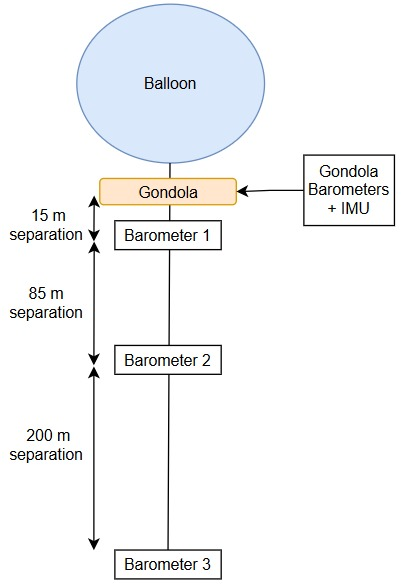
\includegraphics[width=\linewidth]{fig/archB_payload.png}
\caption{Architecture B}
\label{fig:placeholder}
\end{minipage}

\end{figure}

\section{Verification and Validation}

\section{Sensitivity Analysis}

\chapter{ISRU \& Buoyancy Subsystem}\label{chap:ISRU}

% Required packages if not already included in the preamble:
% \usepackage[table]{xcolor}
% \usepackage{tabularx}
% \usepackage{array}
% \usepackage{float}

% If these colours are already defined elsewhere, do not define them twice.
\definecolor{scorefive}{HTML}{B7E1CD}
\definecolor{scorefour}{HTML}{D9EAD3}
\definecolor{scorethree}{HTML}{FCE5CD}
\definecolor{scoretwo}{HTML}{F4CCCC}
\definecolor{scoreone}{HTML}{E6B8AF}

\section{Balloon Design Options Trade-Off}
\label{sec:balloon_design_options_tradeoff}

The design option tree resulted in three straw-man concepts for the lifting and altitude control \cite{baseline_vista}. These concepts were compared to determine whether they are feasible, and to determine which of them would be the most optimal in terms of balloon sizing, gas-processing system, deployment sequence, power demand, reliability, operational complexity, and long-term feasibility. For that, the trade-off has been performed.

\textbf{Option 1:} A large balloon, initially partially filled with helium, and filled with in situ obtained nitrogen over a long period of time, utilising atmospheric CO$_2$ as ballast for altitude control.

\textbf{Option 2:} A filled nitrogen balloon, in situ nitrogen for top-up, altitude controlled using an internal superpressure bladder.

\textbf{Option 3:} A nitrogen balloon, arriving at Venus empty, utilising an internal superpressure bladder for altitude control. A temporary, disposable helium balloon whose purpose is to give the in situ nitrogen extractor enough time to fill the primary balloon.

These are the three options identified and selected in the baseline concept selection. The main mission drivers include the in situ resource utilisation (ISRU) for leakage compensation, power of 500 Wh and total aerobot mass. A full numerical sizing and power estimation have only been developed for Option 2 at this stage. Therefore, the trade-off will be performed using semi-quantitative methods, which still help to clearly establish which concept is the most optimal for the mission purpose. Numerical values for Option 2 will be used where available, such as nitrogen leakage replacement rate, continuous equivalent ISRU power, and altitude-control pump power. For Options 1 and 3, the scores are based on architecture-level metrics that can be evaluated without a full model.

\subsection{Trade-Off Criteria and Weights}
\label{subsec:balloon_trade_criteria}

The selection criteria are selected to match those used in system engineering, such as performance, mass, power, risk, reliability, cost/schedule and sustainability. The criteria, weights, and explanation are shown in Table~\ref{tab:balloon_trade_criteria}.

\begin{table}[H]
\centering
\caption{Balloon design option trade-off criteria and weights.}
\label{tab:balloon_trade_criteria}
\footnotesize
\renewcommand{\arraystretch}{1.12}
\setlength{\tabcolsep}{5pt}
\begin{tabularx}{\textwidth}{@{}p{0.36\textwidth} c X@{}}
\toprule
\textbf{Criterion} & \textbf{Weight} & \textbf{Explanation} \\
\midrule
C1 -- Long-duration lifting robustness 
& 20\%  
& How well can a concept maintain lift for 5 years. \\

C2 -- Power consumption feasibility 
& 20\% 
& Expected gas-processing and altitude-control energy demand. Has to comply with the 500 Wh constraint. \\

C3 -- Deployment and early mission operation risk 
& 15\% 
& Number of potential critical events before stable operation, and to what extent stable operation depends on early ISRU performance. \\

C4 -- Altitude control 
& 15\%  
& Whether the aerobot can maintain and change altitude without losing the lifting gas. \\

C5 -- System complexity 
& 15\%  
& Number of active components such as valves, sensors, pumps, actuators etc. \\

C6 -- Mass and packaging feasibility 
& 10\%  
& Whether the entire system complies with mass constraints. \\

C7 -- Sustainability 
& 5\%  
& Contamination risk. \\
\midrule
\textbf{Total} & \textbf{100\%} & \\
\bottomrule
\end{tabularx}
\end{table}

The weights are chosen as follows, as C1 and C2 are the hardest ones to fulfil. There is not enough representative data about the Venus atmosphere and how it affected the previous missions for prolonged periods of time. C2, on the other hand, is weighted heavily, as the 500 Wh requirement is very strict, and the system must pump and separate kilograms of atmosphere per day for 5 years, meaning it will consume a substantial amount of power. C3, C4 and C5 have been weighted slightly less, as these requirements are slightly clearer, and can be backed up by earlier missions and relevant data. C6 is weighted 0.1, as the system itself is not particularly heavy due to use of advanced materials and hardware, making it less critical. Finally, sustainability is only relevant during the manufacturing process and the end of life, which can also be taken care of later.



\subsection{Trade-Off Table}
\label{subsec:balloon_trade_table}

The final weighted score is calculated as $S_{\mathrm{weighted}} = \sum_i w_i S_i$, where $w_i$ is the criterion weight and $S_i$ is the assigned score between 1 and 5.

The trade-off table is shown in Table~\ref{tab:balloon_tradeoff_table}.

\begin{table}[H]
\centering
\caption{Balloon design options trade-off table.}
\label{tab:balloon_tradeoff_table}
\footnotesize
\renewcommand{\arraystretch}{1.12}
\setlength{\tabcolsep}{5pt}
\begin{tabularx}{\textwidth}{@{}X c c c c@{}}
\toprule
\textbf{Criterion} & \textbf{Weight} & \textbf{Option 1} & \textbf{Option 2} & \textbf{Option 3} \\
\midrule
C1 -- Long-duration lifting robustness 
& 20\% 
& \cellcolor{scorethree}3 
& \cellcolor{scorefive}5 
& \cellcolor{scorethree}3 \\

C2 -- Power consumption feasibility 
& 20\% 
& \cellcolor{scoretwo}2 
& \cellcolor{scorefour}4 
& \cellcolor{scoreone}1 \\

C3 -- Deployment and early mission operation risk 
& 15\%  
& \cellcolor{scorethree}3 
& \cellcolor{scorefive}5 
& \cellcolor{scoretwo}2 \\

C4 -- Altitude control 
& 15\%  
& \cellcolor{scorethree}3 
& \cellcolor{scorefive}5 
& \cellcolor{scorefour}4 \\

C5 -- System complexity 
& 15\%  
& \cellcolor{scorethree}3 
& \cellcolor{scorefour}4 
& \cellcolor{scoretwo}2 \\

C6 -- Mass and packaging feasibility 
& 10\% 
& \cellcolor{scorefour}4 
& \cellcolor{scorethree}3 
& \cellcolor{scorethree}3 \\

C7 -- Sustainability 
& 5\%  
& \cellcolor{scorethree}3 
& \cellcolor{scorefour}4 
& \cellcolor{scoretwo}2 \\
\midrule
\textbf{Total} 
& \textbf{100\%} 
& \textbf{2.90} 
& \textbf{4.40} 
& \textbf{2.40} \\
\bottomrule
\end{tabularx}
\end{table}

\subsection{Score Justification}
\label{subsec:balloon_score_justification}

\textbf{Option 1} scores a decent but not high score of 2.90. It is advantageous as it uses helium initially to keep the balloon afloat, so it does not need to be filled with N$_2$ by the ISRU system immediately after deployment. However, it relies on a gradual transition from helium to nitrogen. Using the power consumption estimation script, at an altitude of 55 km, the system needs a total of approximately 300 kg of nitrogen to stay afloat, split between the superpressure balloon and zero-pressure balloon. To fill it with nitrogen in days, around 5 kg of N$_2$ would need to be pumped per day. According to the preliminary power consumption estimates, this would require about 993.4 W of power during the filling phase, which is not feasible with the 500 Wh energy storage budget unless the filling process is spread over a much longer period. This would decrease the useful mission time.

On top of that, it requires CO$_2$ ballast for altitude control, which adds complexity and creates a more consumable-based control approach. Therefore, it scores lower in system complexity (C5) and altitude-control capability (C4). It scores well in mass and packaging feasibility, as it is only one balloon without extra add-ons.

\textbf{Option 2} scores the highest, with a final score of 4.40. Its main advantage is its simplicity and the fact that it reaches its stable long-term configuration immediately after deployment, as it already contains the nitrogen. The ISRU system is only required for leakage compensation, which, based on the leakage estimation script, is around 185 grams per day as can be seen in \autoref{tab:n2_leakage_summary}. This means that the continuous power consumption of the entire system is about 54 W at maximum leakage rate, according to \autoref{tab:isru_power_results}. This reduces the dependency on early ISRU performance, making the concept more robust for long-duration operation.

Altitude control is performed by means of a superpressure bladder inside the zero-pressure balloon, which is favourable since superpressure volumes provide passive altitude stability. Pumping between pressure volumes is also a known method for changing buoyancy in variable-altitude balloon concepts, which have already been tested before.

It scores lower in mass and packaging, as, for example, to deploy at a 55 km altitude, roughly 300 kg of nitrogen is required, which needs to be brought all the way to Venus. However, this is compensated by the other criteria, making this concept clearly the best choice.

\textbf{Option 3} scores poorly overall, with a final score of 2.40. Despite being a valid concept, it clearly loses on power consumption for the same reason as Option 1, since the main nitrogen balloon still needs to be filled after arrival. It also loses on criteria C3 and C5, as having an extra balloon increases system complexity and adds more risks during deployment and early operation. Moreover, an extra balloon is worse for sustainability, as there will be more material to dispose of at the end of life.

Its altitude-control mechanism concept is reasonable once the main balloon is filled up, but the early-operation risk still dominates the trade-off. Therefore, Option 3 is not selected.

Based on the weighted trade-off, Option 2 is selected as the preferred baseline architecture. Although it has a mass and packaging disadvantage, it provides the best overall balance between long-duration lifting robustness, deployment risk, altitude-control capability and operational simplicity. The selected concept is therefore a filled nitrogen balloon with in situ nitrogen top-up for leakage compensation and an internal superpressure bladder for altitude control.



\definecolor{scorefive}{HTML}{B7E1CD}
\definecolor{scorefour}{HTML}{D9EAD3}
\definecolor{scorethree}{HTML}{FCE5CD}
\definecolor{scoretwo}{HTML}{F4CCCC}
\definecolor{scoreone}{HTML}{E6B8AF}

\section{\texorpdfstring{N$_2$ Separation System Trade-Off}{N2 Separation System Trade-Off}}
\label{sec:n2_separation_tradeoff}

The nitrogen separation system is required to extract N$_2$ from the Venus atmosphere for leakage compensation. Three main methods were considered for the trade-off:

\begin{enumerate}
    \item \textbf{PSA/Molecular Sieve:} uses selective adsorption beds to remove CO$_2$-rich gas and produce an N$_2$-enriched stream. The beds are regenerated by pressure swing.
    \item \textbf{Cryotrapping:} cools the atmospheric feed so that CO$_2$ is frozen out, leaving a more N$_2$-enriched gas stream.
    \item \textbf{Chemical Getters:} uses reactive material to chemically bind or remove CO$_2$, leaving N$_2$ behind.
\end{enumerate}

The considered trade-off criteria are system mass, complexity, power, reliability and Venus environment compatibility. These are selected because the separation system must survive the full mission, fit within the power and mass budget, and operate in the acidic Venus atmosphere.

\subsection{Trade-Off Criteria and Weights}
\label{subsec:n2_trade_criteria}

The criteria, weights, and explanation are shown in Table~\ref{tab:n2_trade_criteria}. Reliability and power are given the highest weights, since failure of the separation system would threaten the whole mission and the onboard energy storage is strongly limited.

\begin{table}[H]
\centering
\caption{N$_2$ separation system trade-off criteria and weights.}
\label{tab:n2_trade_criteria}
\footnotesize
\renewcommand{\arraystretch}{1.12}
\setlength{\tabcolsep}{5pt}
\begin{tabularx}{\textwidth}{@{}p{0.30\textwidth} c X@{}}
\toprule
\textbf{Criterion} & \textbf{Weight} & \textbf{Explanation} \\
\midrule
Reliability 
& 25\% 
& Failure of the separation system will threaten the entire mission. \\

Power 
& 25\%  
& Limited onboard energy storage. \\

Mass 
& 20\%  
& The separation system must fit within a mass budget. \\

Venus Environment 
& 15\%  
& The separation system must survive the acidic atmosphere. \\

Complexity 
& 15\%  
& Affects testing, integration, and increases the number of potential points of failure. \\
\midrule
\textbf{Total} & \textbf{100\%} & \\
\bottomrule
\end{tabularx}
\end{table}

\subsection{Trade-Off Table}
\label{subsec:n2_trade_table}

The final weighted score is calculated as $S_{\mathrm{weighted}} = \sum_i w_i S_i$, where $w_i$ is the criterion weight and $S_i$ is the assigned score.

The trade-off table is shown in Table~\ref{tab:n2_tradeoff_table}. The scores are assigned from 1 to 5, where 5 is the best score.

\begin{table}[H]
\centering
\caption{N$_2$ separation system trade-off table.}
\label{tab:n2_tradeoff_table}
\footnotesize
\renewcommand{\arraystretch}{1.12}
\setlength{\tabcolsep}{5pt}
\begin{tabularx}{\textwidth}{@{}X c c c c c c@{}}
\toprule
\textbf{Method} & \textbf{Reliability} & \textbf{Power} & \textbf{Mass} & \textbf{Venus Env.} & \textbf{Complexity} & \textbf{Total} \\
& \textbf{25\%} & \textbf{25\%} & \textbf{20\%} & \textbf{15\%} & \textbf{15\%} & \\
\midrule
PSA/Molecular Sieve 
& \cellcolor{scorefour}4 
& \cellcolor{scorethree}3 
& \cellcolor{scorefour}4 
& \cellcolor{scoretwo}2 
& \cellcolor{scorethree}3 
& \textbf{3.30} \\

Cryotrapping 
& \cellcolor{scoretwo}2 
& \cellcolor{scoreone}1 
& \cellcolor{scoretwo}2 
& \cellcolor{scoretwo}2 
& \cellcolor{scoretwo}2 
& \textbf{1.75} \\

Chemical Getters 
& \cellcolor{scorethree}3 
& \cellcolor{scorefour}4 
& \cellcolor{scoreone}1 
& \cellcolor{scoretwo}2 
& \cellcolor{scorefour}4 
& \textbf{2.85} \\
\bottomrule
\end{tabularx}
\end{table}

\subsection{Score Justification}
\label{subsec:n2_score_justification}

\textbf{PSA/Molecular Sieve} receives the highest score. Its main advantage is that it is a regenerable separation method, meaning that the adsorbent beds can be reused, instead of carrying a large consumable mass. PSA/molecular sieves are also a known technology, which has strong industrial heritage, therefore scoring high in reliability. It is not a passive system in terms of power, since valves operation and feed compression are required, which also increases the complexity. However, it is still much less power-consuming and less complex compared to cryotrapping. The Venus environment score is moderate because the sieve beds must still be protected from sulfuric acid aerosols by filters or inlet protection. Finally, the mass score is relatively high compared to chemical getters and cryotrapping, since PSA avoids a large consumable mass and does not require a full cooling system.

\textbf{Cryotrapping} receives the lowest score. First, its main disadvantages are power consumption and mass. Since it needs to constantly cool a large amount of gas, it would require a cryocooler, heat exchangers, insulation and thermal rejection hardware, making it highly demanding in both power and mass, as well as increasing system complexity, which also reduces the score. It also scores poorly in Venus environment compatibility for the same reason as PSA, as sulfuric acid aerosols and contaminants can deposit on cold surfaces or worsen clogging.

\textbf{Chemical getters} receive a moderate score. Their main advantage is simplicity. Power consumption is much lower compared to PSA and cryotrapping, hence it scores well in both power and system complexity. This advantage however only holds when the getter is treated as a consumable, meaning major mass concerns will arise. Since N$_2$ is only 3.5\% of the atmosphere, the CO$_2$ mass that must be removed is roughly:
\begin{align}
    \frac{m_{\mathrm{CO_2}}}{m_{\mathrm{N_2}}}
    =
    \frac{0.965 \cdot 44}{0.035 \cdot 28}
    \approx 43
\end{align}
Therefore, for 185 grams of N$_2$, about 8 kg of CO$_2$ must be removed daily, which corresponds to over 14 tonnes of CO$_2$ over a 5-year mission duration. This makes the technology infeasible from a mass point of view. On the other hand, if the getter were made regenerable, it would lose much of its simplicity and would require extra power and regeneration hardware, making it closer to PSA but with less heritage.


Based on the weighted trade-off, PSA/Molecular Sieve is selected as the preferred nitrogen separation method. Although it is not passive and still requires valves, a feed compressor and inlet protection, it provides the best overall balance between reliability, power, mass, complexity and Venus environment compatibility.

\section{Balloon Material Options Trade-Off}

\noindent The balloon envelope is the most operationally sensitive structural element of the VISTA aerobot. Unlike terrestrial or even stratospheric balloon envelopes, the Venus cloud-layer environment simultaneously imposes several requirements that no single polymer film can satisfy individually \cite{yung2024planetaryvenus}. The outer surface must resist concentrated sulphuric acid aerosols H$_2$SO$_4$ \cite{delitsky2023cloudchemistryvenus}, the gas-barrier layer must suppress nitrogen leakage over a five-year float duration, the load-bearing layer must sustain superpressure-driven hoop stresses at 55\,km altitude, and every component must remain mechanically sound through interplanetary cruise, deployment shock, and multi-year thermal cycling \cite{Hall2007_VenusPrototype,Hall2009_SecondGen,Hall2011_TechDev}. 
\medskip

\noindent This chapter presents the material trade-off analysis and refilling mechanism selection process for the VISTA balloon dome. Section \ref{sec:operational-and-req} characterises the environmental loads and derives the material-level requirements. Section \ref{sec:mat-candidates} reviews the candidate materials at the individual film level, covering acid resistance, gas permeability, tensile properties, density, and brittleness at operational conditions. Section \ref{sec:mat-architectures} extends the analysis to multi-layer laminate architectures that might combine desired properties. Section \ref{sec:mat-tradeoff} presents the scored trade-off and section \ref{sec:mat-selection} states the selected architecture and justifies the selection against the mission constraints.

\section{Operational Conditions and Requirements}\label{sec:operational-and-req}

First, the operational environment must be revisited. Then, its take-aways will be used to express subsystem-specific requirements flowing down from system-level VISTA requirements \cite{baseline_vista}.

\subsection{Environmental Loads at the Float Altitude}
\label{sec:mat-environment}

The VISTA float altitude of approximately 55\,km sits within the main Venusian cloud layer. The relevant environmental parameters for envelope material selection are summarised in Table \ref{tab:float-environment}. At this altitude, the atmospheric temperature is approximately 27-37\,$^\circ$C and the pressure is approximately 0.4-0.5\,bar. These conditions are mild in comparison to the Venus surface, but the sulphuric acid environment is uniquely aggressive: cloud droplets of H$_2$SO$_4$ are present continuously at 49-57\,km \cite{Knollenberg1980_VenusAerosol}. During descent and inflation, the envelope may encounter higher acid concentrations and steeper temperature gradients that also have to be accounted for. The design must also consider solar UV irradiance on the dayside, which is relevant to materials with photosensitive bond chemistry.

\begin{table}[H]
\centering
\caption{Environmental parameters at the VISTA float altitude (55\,km) relevant to envelope material selection.}
\label{tab:float-environment}
\footnotesize
\renewcommand{\arraystretch}{1.15}
\setlength{\tabcolsep}{5pt}
\begin{tabularx}{\linewidth}{@{}p{3.35cm} p{2.6cm} X@{}}
\toprule
\textbf{Parameter} & \textbf{Value} & \textbf{Design significance} \\
\midrule
Temperature & 27-37\,$^\circ$C & Within polymer service range; critical for acid reaction kinetics. \\
Pressure & $\approx$0.46\,bar & Superpressure differential $\Delta p \approx$2-4\,kPa drives hoop stress. \\
H$_2$SO$_4$ concentration & 75-85\,wt\% & Attacks polyesters, polyamides, and most non-fluorinated organics. \\
H$_2$SO$_4$ exposure duration & $\geq$5 years continuous & Eliminates short-term acid-resistant coatings; requires inherently inert chemistry. \\
Dayside UV & $\sim$3$\times$ terrestrial & Degrades UV-sensitive polymer chains. \\
Night temperature swing & $\pm$20\,$^\circ$C per cycle & Drives thermal fatigue in laminates with mismatched CTE. \\
Lifting gas & Nitrogen (in situ) & Lower permeability kinetic diameter (0.364\,nm) than H$_2$ (0.289\,nm) \cite{PolyimideGasTransport2024}. \\
Float duration & $\geq$5 years & $\approx$365 atmospheric circumnavigation cycles; $\approx$1825 days of acid exposure. \\
\bottomrule
\end{tabularx}
\end{table}

\noindent One important design consequence of the nitrogen-ISRU architecture is that the driver for leaking considerations is nitrogen permeability through the envelope, not helium permeability as in the JPL helium-based prototypes \cite{Hall2007_VenusPrototype,Hall2009_SecondGen}. Because the kinetic diameter of N$_2$ (0.364\,nm) is larger than that of He (0.26\,nm) or H$_2$ (0.289\,nm), nitrogen permeates through most polymer films at a substantially lower rate than noble helium or small-diameter dihydrogen molecules. This is a structural advantage of the VISTA nitrogen architecture from a material perspective. Mainly, laminates that failed to contain helium over months may retain nitrogen for multi-year operation, and materials that were proven in retaining helium will provide a reliability margin for a less constraining in this regard nitrogen-based design \cite{Sebok2015_PTFEpermeability}.

\subsection{Derived Material-Level Requirements}
\label{sec:mat-requirements}

From the top-level mission requirements (Baseline Review \cite{baseline_vista} and the environmental characterisation above, the following material-level derived requirements are identified for the balloon envelope:

\begin{table}[H]
\centering
\small
\caption{Envelope Material Requirements}
\begin{tabular}{|l|p{3.5cm}|p{9cm}|}
\hline
\textbf{ID} & \textbf{Name} & \textbf{Requirement Statement} \\ \hline

REQ-MAT-01 & Acid resistance & The outer surface shall exhibit no measurable loss of mechanical integrity after 5-year continuous exposure to operational H$_2$SO$_4$ concentration at 55 km above the Venusian surface. \\ \hline

REQ-MAT-02 & Nitrogen gas retention & The total envelope nitrogen permeance shall be such that the steady-state leakage loss can be replaced by the in situ nitrogen replenishment system at a rate consistent with the power budget allocation to the ISRU subsystem. \\ \hline

REQ-MAT-03 & Tensile strength & The envelope areal tensile load capacity shall provide a safety factor of $\geq 3$ against the worst-case superpressure burst load of $\Delta p \approx 39{,}200\,\mathrm{Pa}$ for a sphere of radius $R$, where the hoop stress is $\sigma = \Delta p \cdot R / (2t)$ \cite{Hall2007_VenusPrototype}. \\ \hline

REQ-MAT-04 & Areal mass density & The envelope areal density $\sigma$ shall not exceed 150\,g/m$^2$ for the nominal design case. \\ \hline

REQ-MAT-05 & Non-brittleness and flex tolerance & The material shall survive the stowed and packaged configuration during launch and the aerial deployment without pinhole formation or delamination. This implies a minimum elongation at break of $\geq 2\%$ and a minimum flex fatigue life of 1000 cycles without loss of gas-barrier integrity. \\ \hline

REQ-MAT-06 & UV and thermal stability & The material shall retain $\geq 80\%$ of its initial tensile strength after 5 years of dayside UV exposure at Venus irradiance levels and after 1825 diurnal temperature cycles of $\pm 40\,^\circ$C amplitude. \\ \hline

REQ-MAT-07 & TRL & All constituent materials shall have a TRL of at least 4 in relevant environments, aligned with project's general TRL floor. \\ \hline

\end{tabular}
\label{tab:material_requirements}
\end{table}


\iffalse
\section{Individual Candidate Material Assessment}
\label{sec:mat-candidates}

The candidate materials are assessed here at the individual film or fabric level before combined laminate architectures are constructed in Section \ref{sec:mat-architectures}. Each candidate is evaluated against the six material-level criteria: acid resistance, N$_2$ gas permeability, tensile strength per unit areal density, brittleness, UV and thermal stability, and heritage/TRL. An effort was made to rely on available quantitative data, but if only relative comparisons are available from the Venus aerobot literature, the rating is qualitative.


\subsection{Polytetrafluoroethylene (PTFE) Film}
\label{ssec:ptfe}

PTFE was the outer layer of the original Vega balloon envelopes, where it demonstrated flight-proven acid resistance at the Venus cloud level \cite{Kremnev1986}. Its fully fluorinated carbon backbone renders it essentially inert to sulphuric acid, and the material shows no measurable degradation in tensile properties after immersion in H$_2$SO$_4$ present in Vanusian clouds \cite{FosterMiller1996_PBOVenus}. PTFE is also chemically stable under the UV spectrum relevant to Venus.

\begin{figure}[H]
    \centering
    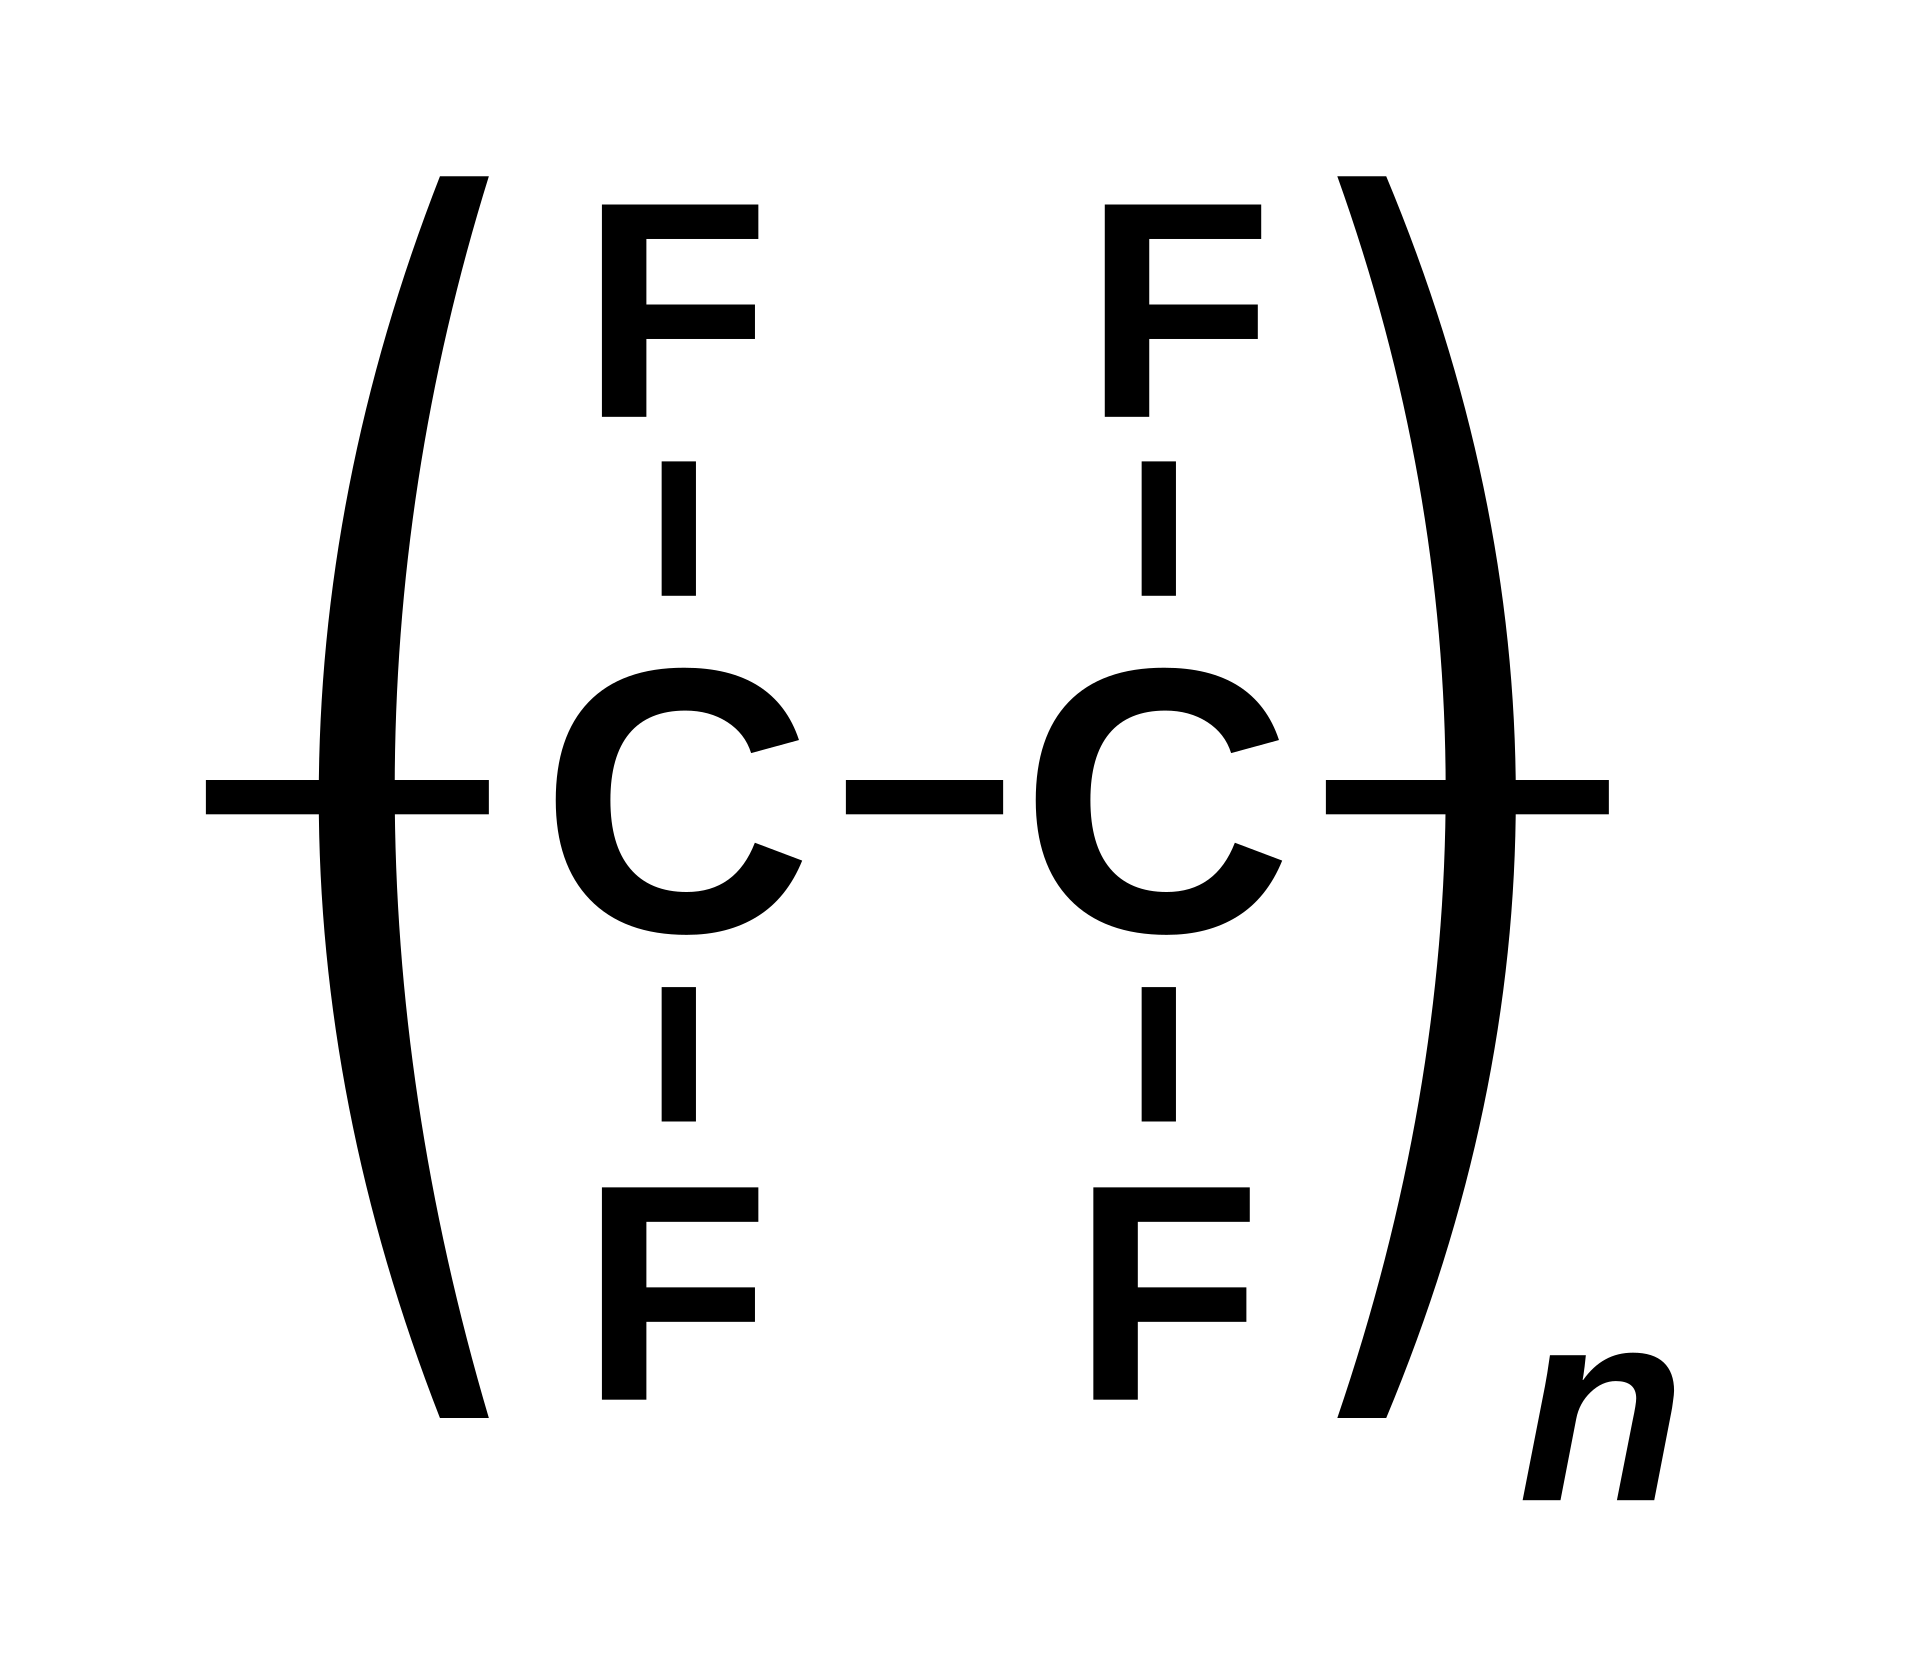
\includegraphics[width=0.18\linewidth]{fig/PTFE.png}
    \caption{Molecular Structure of PTFE}
    \label{fig:PTFE}
\end{figure}

\noindent The gas permeability of a 0.1\,mm PTFE membrane has been quantitatively characterised by Seb\"{o}k et al., who report that H$_2$ permeability through PTFE is substantially higher than N$_2$ permeability: the diffusivity ranking shows $D_{H_2} \gg D_{N_2}$ across the range from room temperature to 180\,$^\circ$C, which is consistent with difference in kinetic diameters of considered molecules (N$_2$ has a kinetic diameter of 0.364\,nm versus H$_2$ at 0.289\,nm) \cite{Sebok2015_PTFEpermeability}. For the VISTA nitrogen-ISRU architecture this is favourable, as it proves N$_2$ permeates through PTFE at a substantially lower rate than H$_2$ would under identical conditions - once again highlighting the reliability margin of helium permeability findings, mentioned in Section \ref{sec:mat-environment}. Moreover, comparative fluoropolymer gas permeability data place PTFE nitrogen permeability at $\sim$10\,cm$^3$/m$^2$/d/bar, substantially lower than PFA (500\,cm$^3$/m$^2$/d/bar) or FEP (1200\,cm$^3$/m$^2$/d/bar) at the same thickness \cite{PCTFE_Permeability_Guide}.

\medskip

\noindent This laminate is not without its weaknesses, though. PTFE film is mechanically weak when unsupported. It has a relatively low tensile strength (20-35\,MPa depending on sintering condition) and does not withstand repetitive folding without developing microcrack networks \cite{FEPwiki}. It cannot be melt-processed and therefore cannot be heat-seamed, which is a practical limitation for gore-seam construction of the balloon dome \cite{FluorocarbonPTFEvsPFA}. PTFE film is therefore best used as an outer protective layer and not as the primary structural element.

\subsection{Perfluoroalkoxy Polymer (PFA) Film}
\label{ssec:pfa}

PFA shares PTFE's fully fluorinated chemistry (see Figure \ref{fig:PFA}) and therefore its good acid resistance, but has an advantage of being melt-processible and heat-welded \cite{FluorocarbonPTFEvsPFA}. This makes it more practical for seam construction than PTFE film. JPL specifically proposed PFA as an alternative protective outer-layer fluoropolymer for Venus aerobot applications \cite{FosterMiller1996_PBOVenus}. Its continuous service temperature extends to approximately 260\,$^\circ$C, well above the Venus cloud-level conditions.

\begin{figure}[H]
    \centering
    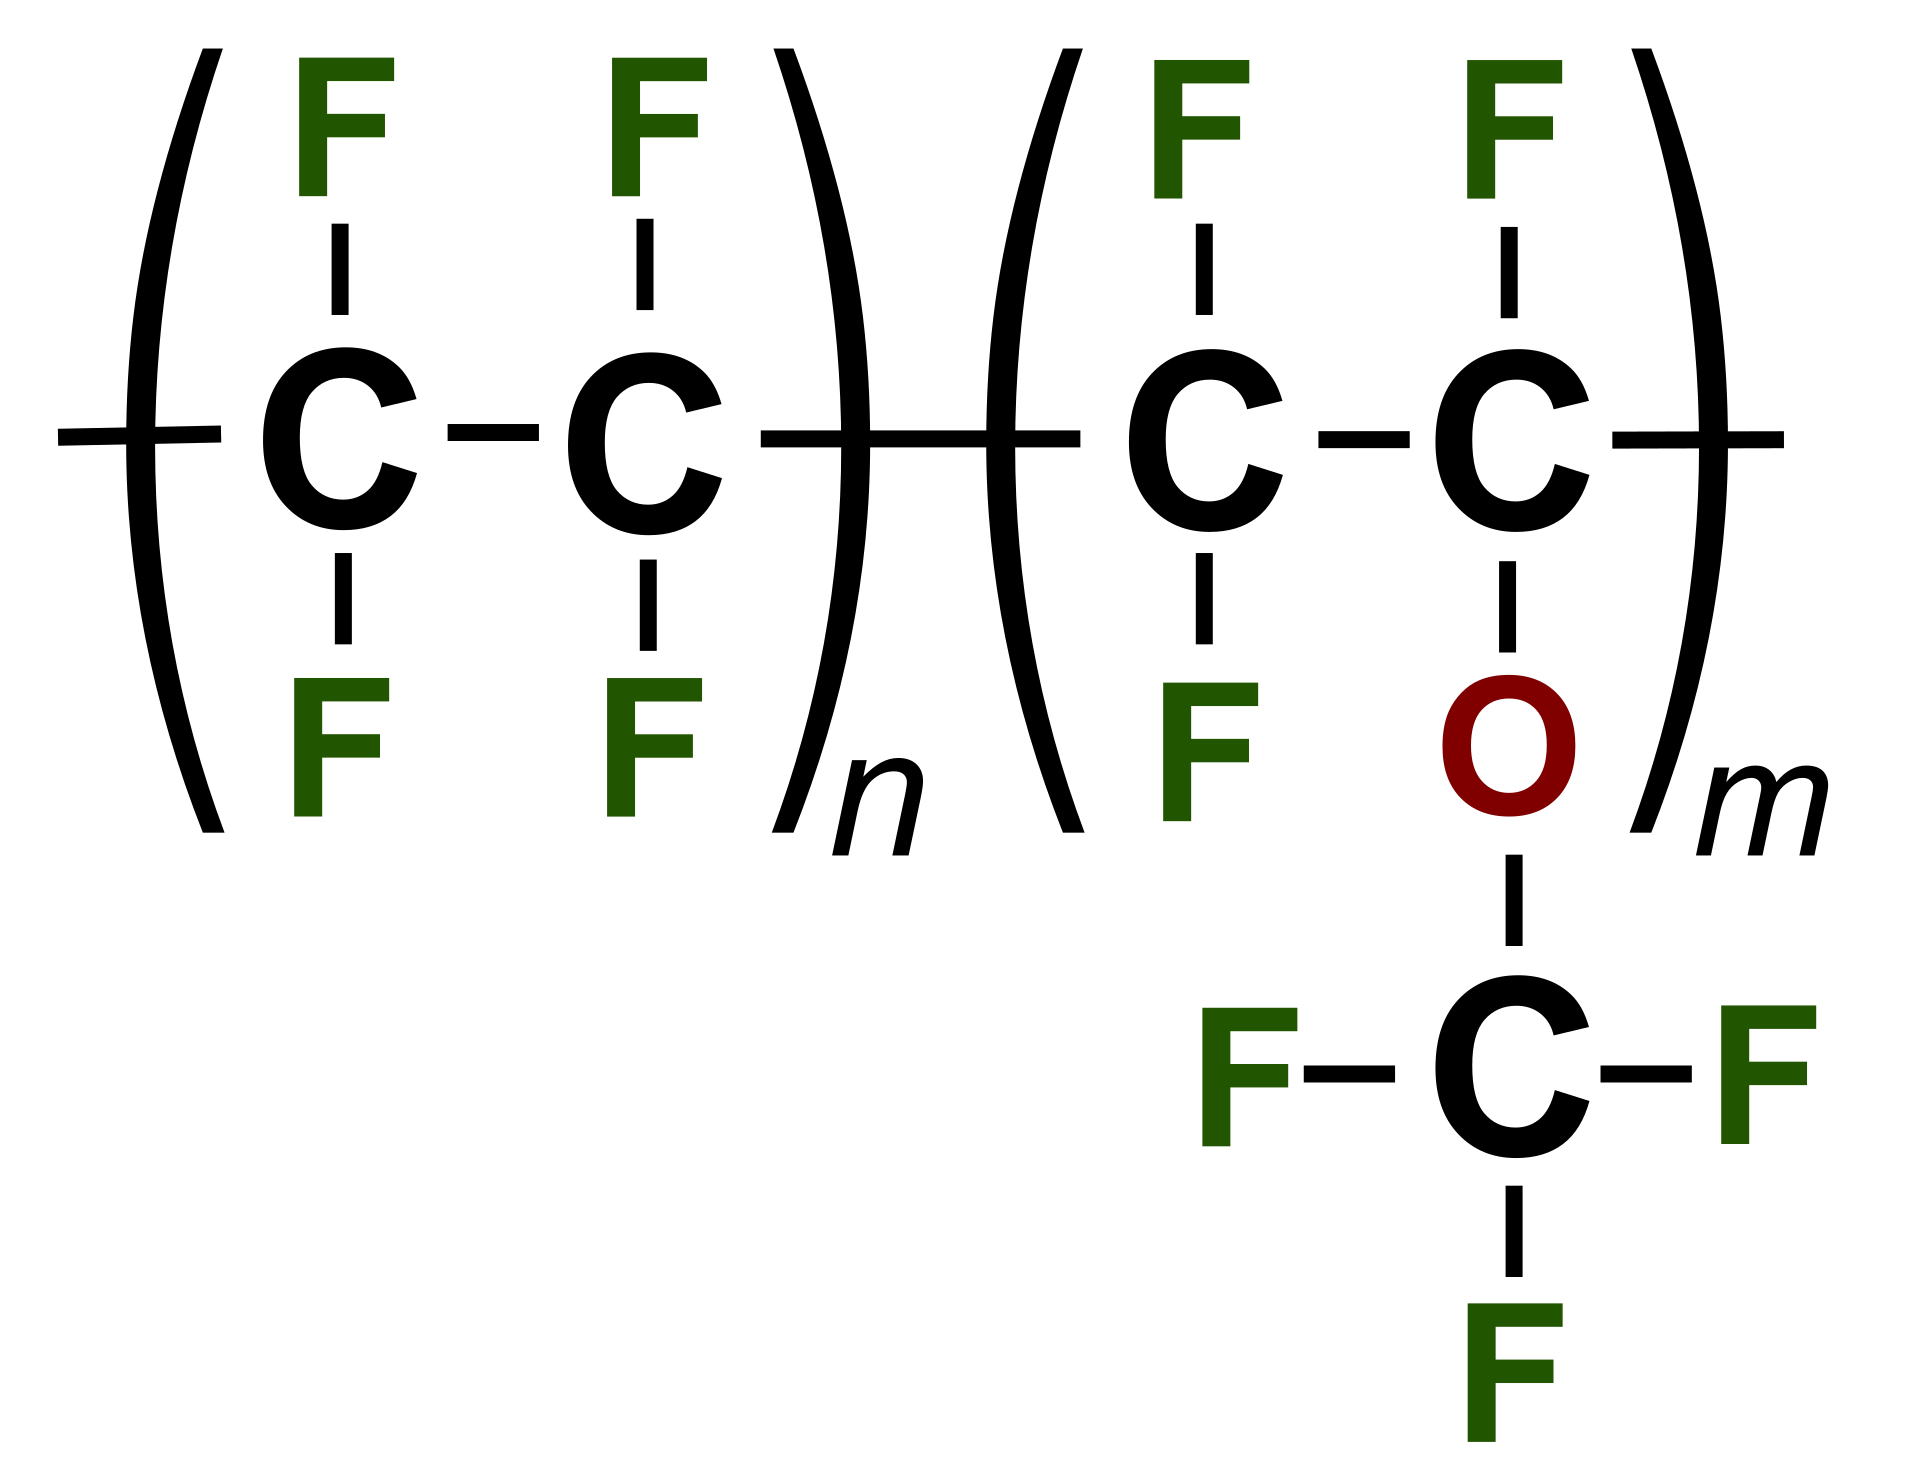
\includegraphics[width=0.25\linewidth]{fig/PFA.png}
    \caption{Molecular Structure of PFA}
    \label{fig:PFA}
\end{figure}

\noindent PFA's N$_2$ permeability is higher than PTFE at the same thickness, due to PFA's lower crystallinity and larger free volume within the polymer matrix \cite{PCTFE_Permeability_Guide,FEP_PFA_permeability}. In a gas-barrier role, PFA is therefore inferior to PTFE, though it still outperforms polyimide films by roughly an order of magnitude. PFA's tensile strength is similar to PTFE (25-30\,MPa), and it is likewise not usable as a structural load-bearing layer without a fabric substrate. Its flex life is better than sintered PTFE due to the melt-processible microstructure. Therefore, whether PTFE or PFA will be used will largely depend on combination of other materials in the multi-layer architectures considered, and what remaining parameters will be of highest importance for successful combined performance.


\subsection{Fluorinated Ethylene Propylene (FEP) Film}
\label{ssec:fep}

FEP was the outer layer of the first JPL Venus balloon prototype \cite{Hall2007_VenusPrototype}. It is chemically similar to PTFE and PFA, as shown in the Figure \ref{fig:FEP}, and melts at approximately 260\,$^\circ$C, enabling film extrusion and heat-seaming. FEP is slightly softer than PTFE and does not withstand repetitive folding as well \cite{FEPwiki}. Its N$_2$ permeability is at approximately 1200\,cm$^3$/m$^2$/d/bar, making it a weaker gas barrier than both PTFE and PFA at equivalent thickness \cite{PCTFE_Permeability_Guide}. 

\begin{figure}[H]
    \centering
    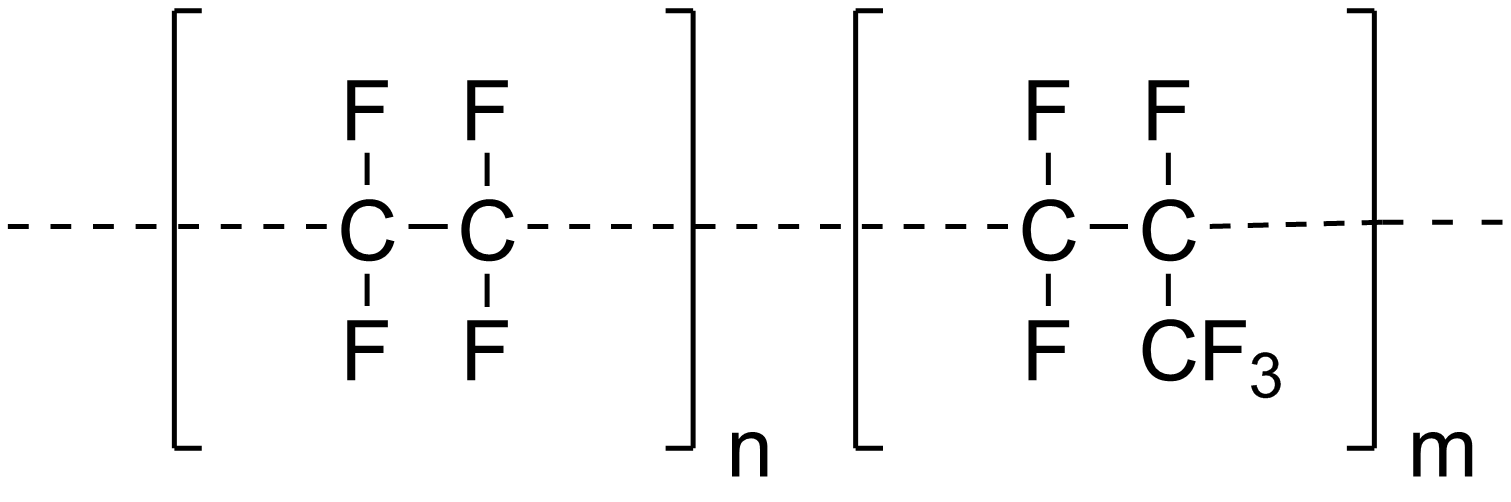
\includegraphics[width=0.5\linewidth]{fig/FEP.png}
    \caption{Molecular Structure of FEP}
    \label{fig:FEP}
\end{figure}

\noindent FEP in the aluminized form was used as the outer layer in the JPL Gen-1 laminate: aluminized Teflon FEP / aluminized Mylar / Vectran / polyurethane \cite{Hall2007_VenusPrototype}. In this configuration FEP provides acid resistance and solar reflectivity (via the aluminium coating), while gas barrier duty is delegated to the aluminized Mylar layer. FEP was later replaced by Aclar (PCTFE) in the Gen-2 laminate due to Aclar's superior toughness and abrasion resistance during handling \cite{Hall2011_TechDev}.



\subsection{Polychlorotrifluoroethylene (PCTFE) - Aclar Film}
\label{ssec:pctfe}


PCTFE (commercially Aclar) is a partially fluorinated polymer with a chlorine substituent on every other carbon along the backbone. It is presented in the Figure \ref{fig:PCTFE}:

\begin{figure}[H]
    \centering
    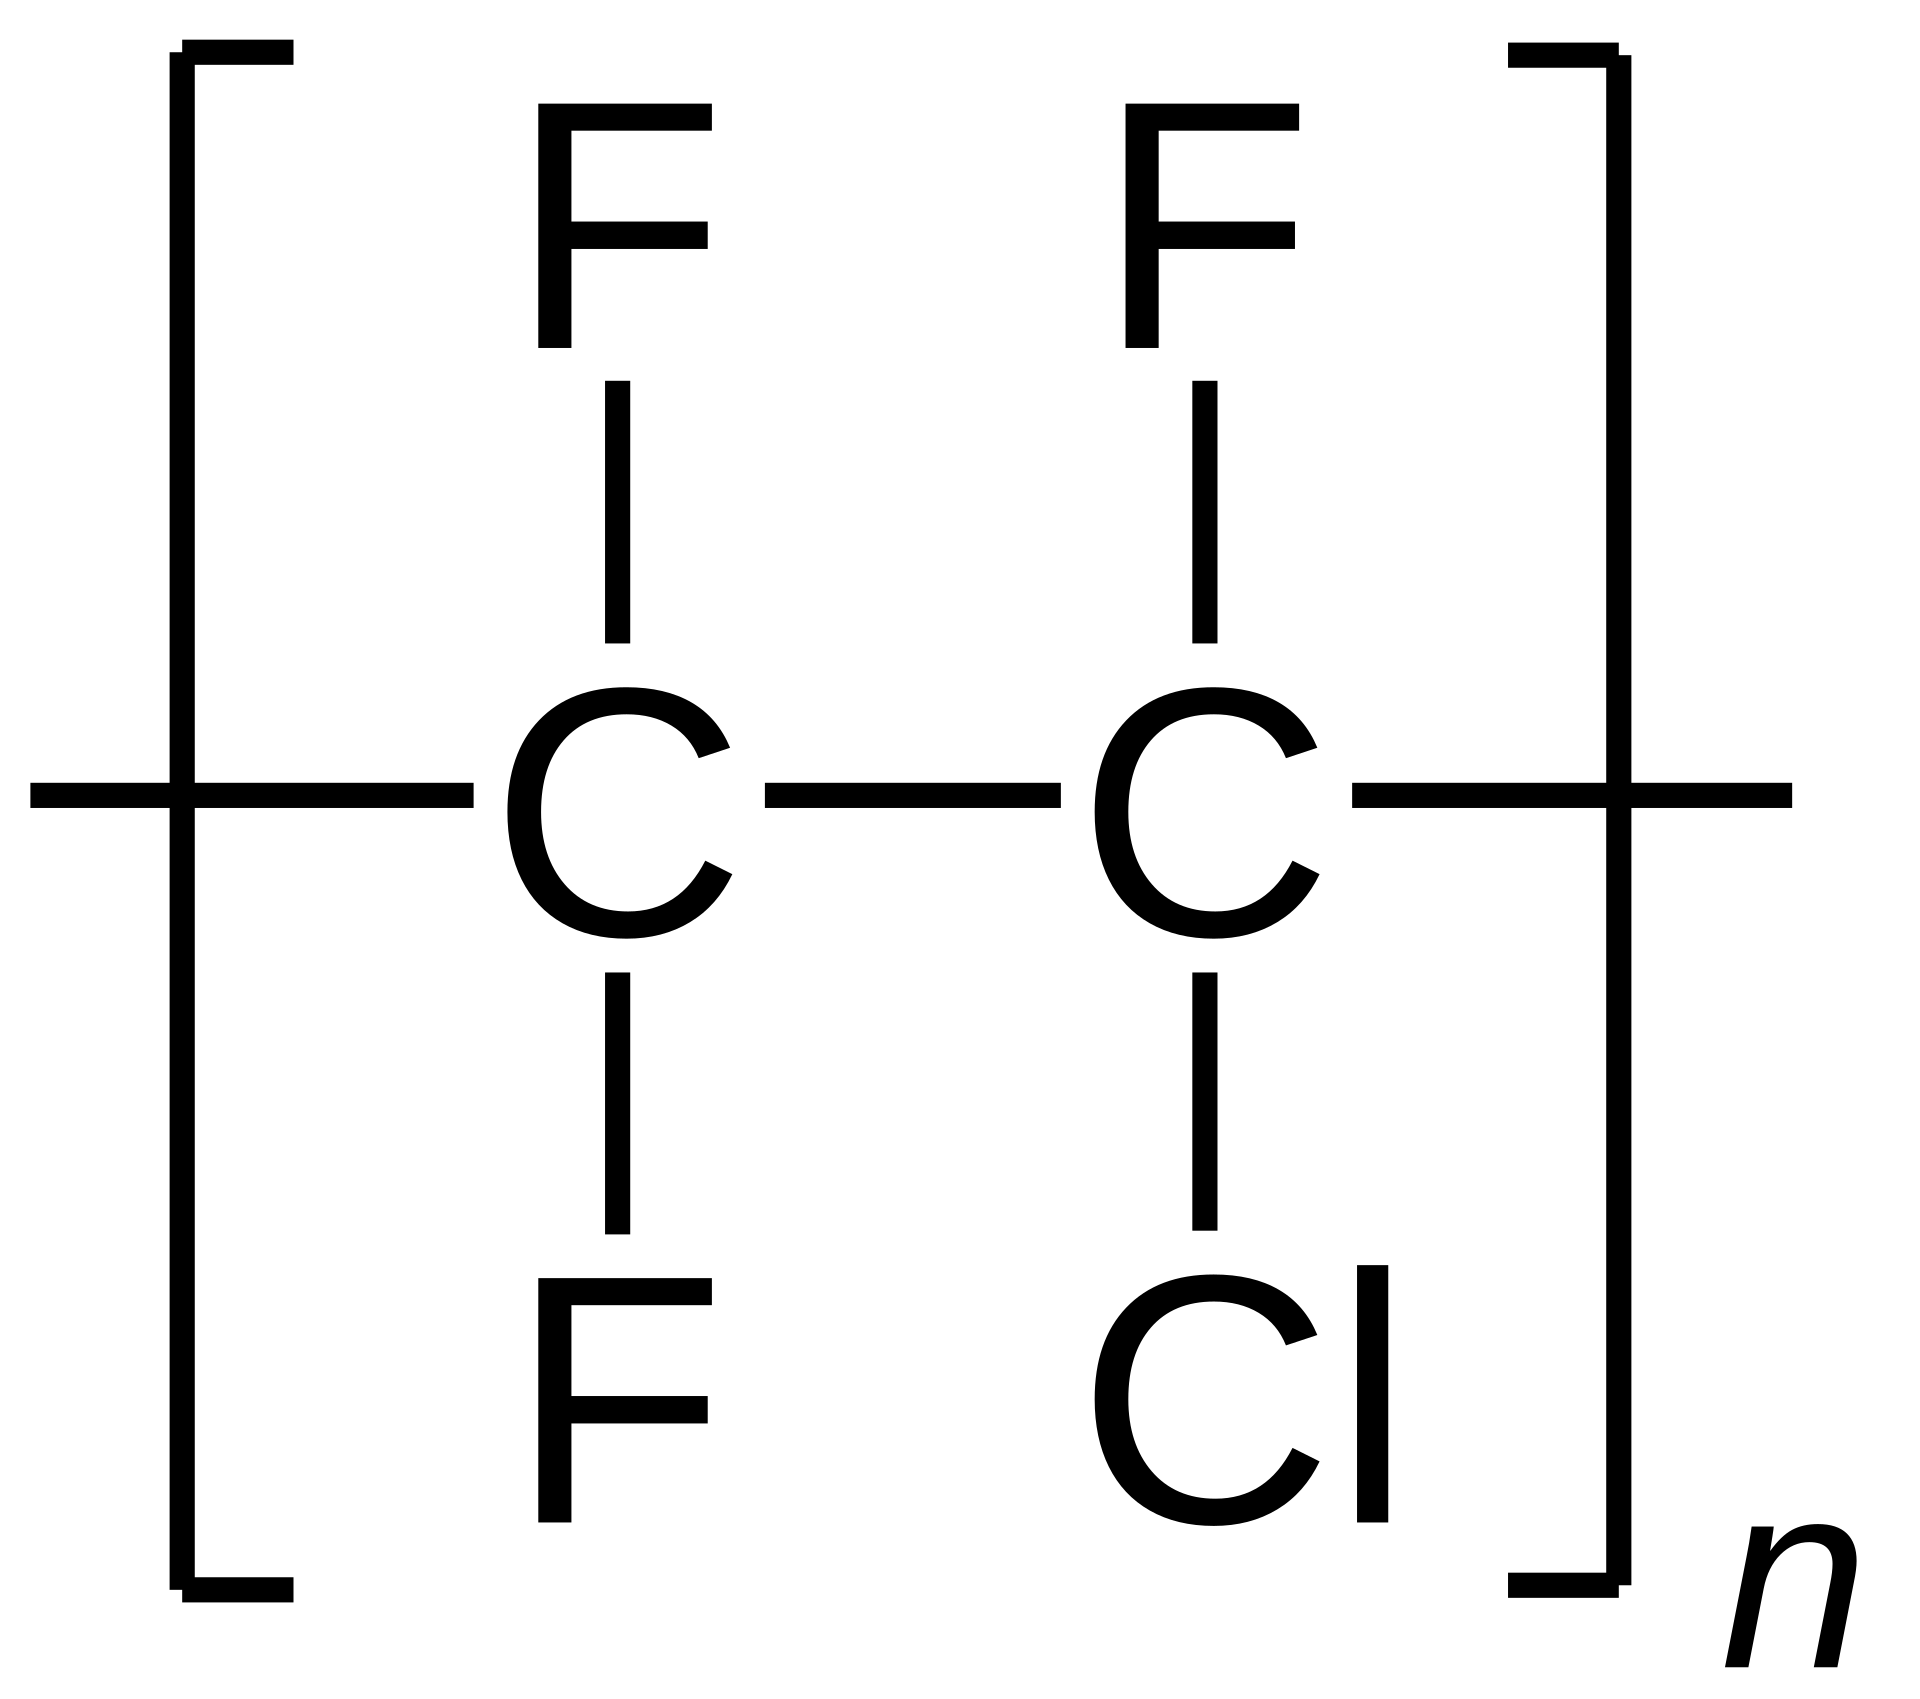
\includegraphics[width=0.17\linewidth]{fig/PCTFE.png}
    \caption{Molecular Structure of PCTFE}
    \label{fig:PCTFE}
\end{figure}

\noindent This structural feature results in significantly higher crystallinity than PFA or FEP, which suppresses chain-segment mobility and drastically reduces gas permeability. Among all commercially available fluoropolymers at useful film thicknesses, PCTFE has the lowest gas permeability: N$_2$ permeability is approximately 10\,cm$^3$/m$^2$/d/bar at 25\,µm thickness, comparable to PTFE but in a melt-processible form \cite{PCTFE_Permeability_Guide}. Its H$_2$O vapour permeability is the lowest of any commercial transparent film.

\medskip

\noindent JPL introduced Aclar as the outer film in the Gen-2 Venus balloon laminate precisely because it combines superior gas barrier performance with better abrasion resistance and toughness than FEP \cite{Hall2011_TechDev}. Aclar has a service temperature of approximately 120\,$^\circ$C (limited by the chlorine-containing backbone relative to fully fluorinated alternatives) and acceptable acid resistance at Venus cloud conditions. Its elongation at break is 100-250\%, giving it better flex tolerance than PTFE film \cite{AclarBarrierFilms}.

\medskip

\noindent The primary limitation of PCTFE is that the chlorine atom slightly reduces its chemical inertness relative to pure fluoropolymers: prolonged exposure to very strong reducing agents can break the C-Cl bond. However, at the Venus cloud-level H$_2$SO$_4$ presence (an oxidising rather than reducing acid), this is not considered a failure mode.



\subsection{Biaxially Oriented Polyethylene Terephthalate (BoPET) - Mylar Film}
\label{ssec:mylar}

Mylar (BoPET) is the standard gas-barrier film for terrestrial and planetary balloon applications, shown in the Figure \ref{fig:BoPET}:

\begin{figure}[H]
    \centering
    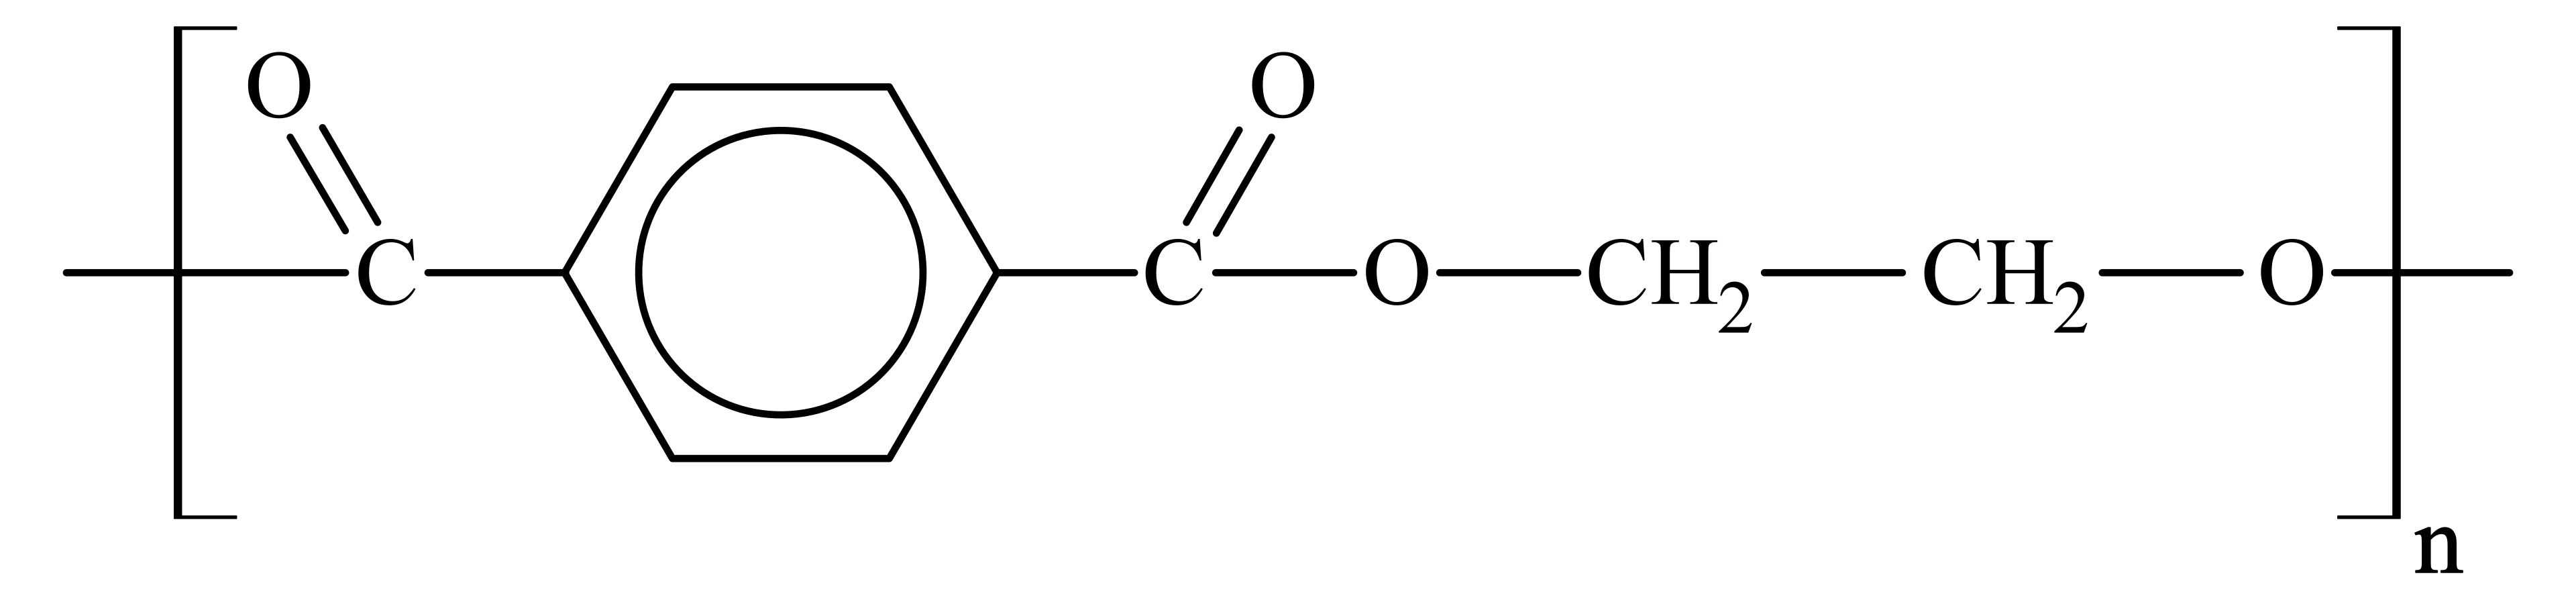
\includegraphics[width=0.6\linewidth]{fig/BoPET.png}
    \caption{Molecular Structure of BoPET}
    \label{fig:BoPET}
\end{figure}

Its gas barrier performance in the metallised form (typically 25-75\,nm vacuum-deposited Al layer) approaches that of a continuous metal film for large gas molecules, but metalised Mylar is susceptible to pinhole formation during flexing \cite{MetallizedFilmFlex}. Without metallisation, BoPET has a N$_2$ permeability far too high for multi-year mission. Moreover, which is critical for the given application, the uncoated BoPET is attacked and dissolved by concentrated sulphuric acid \cite{FosterMiller1996_PBOVenus}, which renders it unsuitable for use as an outer layer at Venus. In the Gen-1 JPL laminate, Mylar was retained as an intermediate gas-barrier layer protected from acid contact by the outer FEP layer \cite{Hall2007_VenusPrototype}, which allows to use its benefits while minimising the impact of its weaknesses. 

\medskip

\noindent In the Gen-2 laminate, aluminized Mylar was replaced by thin aluminium foil, which provides a dramatically better helium (and by extension nitrogen) barrier: continuous aluminium foil is impermeable to all gases when free of pinholes, and foil pinholes can be suppressed by lamination tension control and proper seam design \cite{Hall2011_TechDev}. Aluminium foil at 8-12\,µm thickness contributes approximately 20-25\,g/m$^2$ to the laminate areal density, far less than the metallization-plus-Mylar combination for equivalent barrier performance.





\subsection{Vectran Fabric}
\label{ssec:vectran}

Vectran, a liquid-crystal aromatic polyester, poly(hydroxybenzoic acid-co-2-hydroxy-6-naphthoic acid) in the Figure \ref{fig:vectran}, is the structural load-bearing fabric in both JPL Venus balloon prototypes \cite{Hall2007_VenusPrototype,Hall2009_SecondGen}. 

\begin{figure}[H]
    \centering
    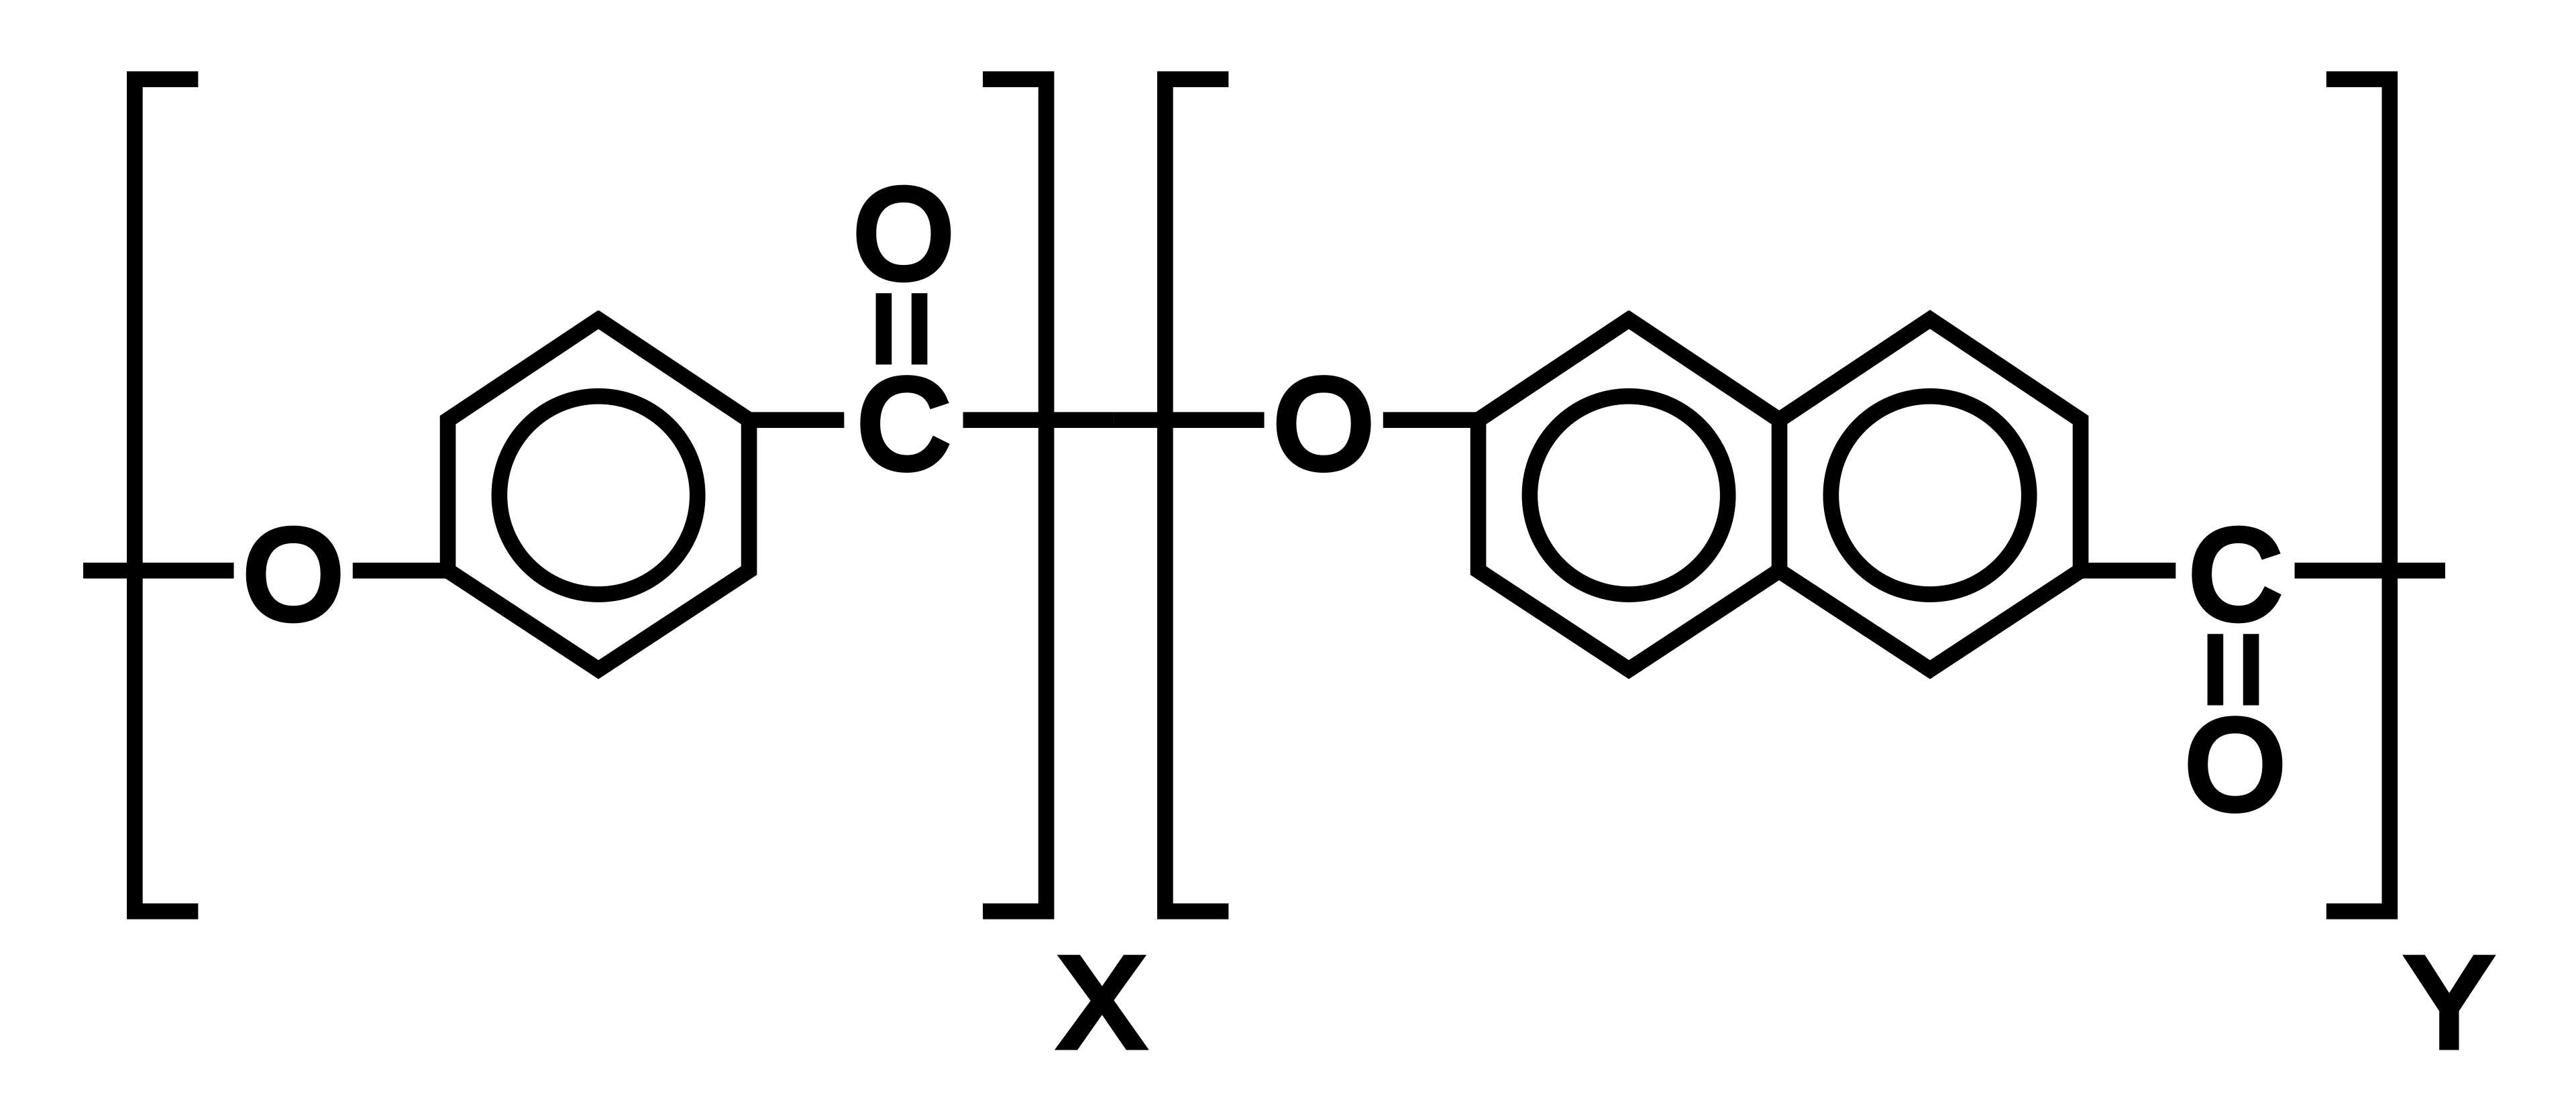
\includegraphics[width=0.5\linewidth]{fig/vectran.png}
    \caption{Molecular Structure of Vectran}
    \label{fig:vectran}
\end{figure}

\noindent As a thermotropic LCP fibre, Vectran's molecular chains are oriented along the fibre axis during melt spinning, giving it tensile strength of approximately 2.9\,GPa and tensile modulus of approximately 70-130\,GPa depending on grade \cite{VectranReview2021}. On a weight-relative basis it is five times stronger than steel \cite{VectranFibrXL}. 

\medskip

\noindent Vectran's thermal performance is well-characterised: it has a melting point of 330\,$^\circ$C and exhibits progressive strength loss above 220\,$^\circ$C, but at the Venus cloud-deck temperature of 35\,$^\circ$C its tensile properties increase slightly relative to ambient temperature. Specifically, its strength increases by approximately +20\% compared to sub-zero temperatures \cite{VectranImattec}. Critically for multi-year superpressure service, Vectran exhibits negligible creep under loads up to 50\% of its breaking strength \cite{VectranFibrXL}, which is the key advantage over para-aramid (Kevlar) fibres in this application.

\medskip

\noindent Vectran is an aromatic polyester; like BoPET, neat Vectran fibre can be attacked by concentrated sulphuric acid if unprotected. In laminate practice, Vectran is always the middle or inner layer, fully encapsulated between the acid-resistant outer film and the inner polyurethane coating, and is therefore never in direct acid contact.

\medskip

\noindent Vectran has a known UV sensitivity, similar to other rigid-rod LCP fibres \cite{VectranImattec}. This is managed in the laminate by the UV-opaque outer fluoropolymer and aluminium layers, which prevent photon access to the Vectran layer.



\subsection{Polybenzoxazole (PBO) - Zylon Film and Fabric}
\label{ssec:pbo}

PBO is a rigid-rod, thermoset liquid-crystalline polymer fibre with the highest tensile strength of any commercially marketed organic fibre at 5.8\,GPa with modulus up to 270\,GPa \cite{ZylonTechnical2005,ZylonSciDirect}. Its limiting oxygen index of 68 and decomposition temperature above 650\,$^\circ$C make it thermally exceptional for Venus applications.

\medskip
\noindent However, PBO has several critical weaknesses for the VISTA concept. First, PBO/Zylon fibres suffer rapid and irrecoverable strength loss under exposure to UV radiation and even visible light \cite{ZylonWiki,ZylonFiberLine}. The mechanism is photodegradation of the benzobisoxazole ring C=N bonds, shown in the Figure \ref{fig:PBO}.


\begin{figure}[H]
    \centering
    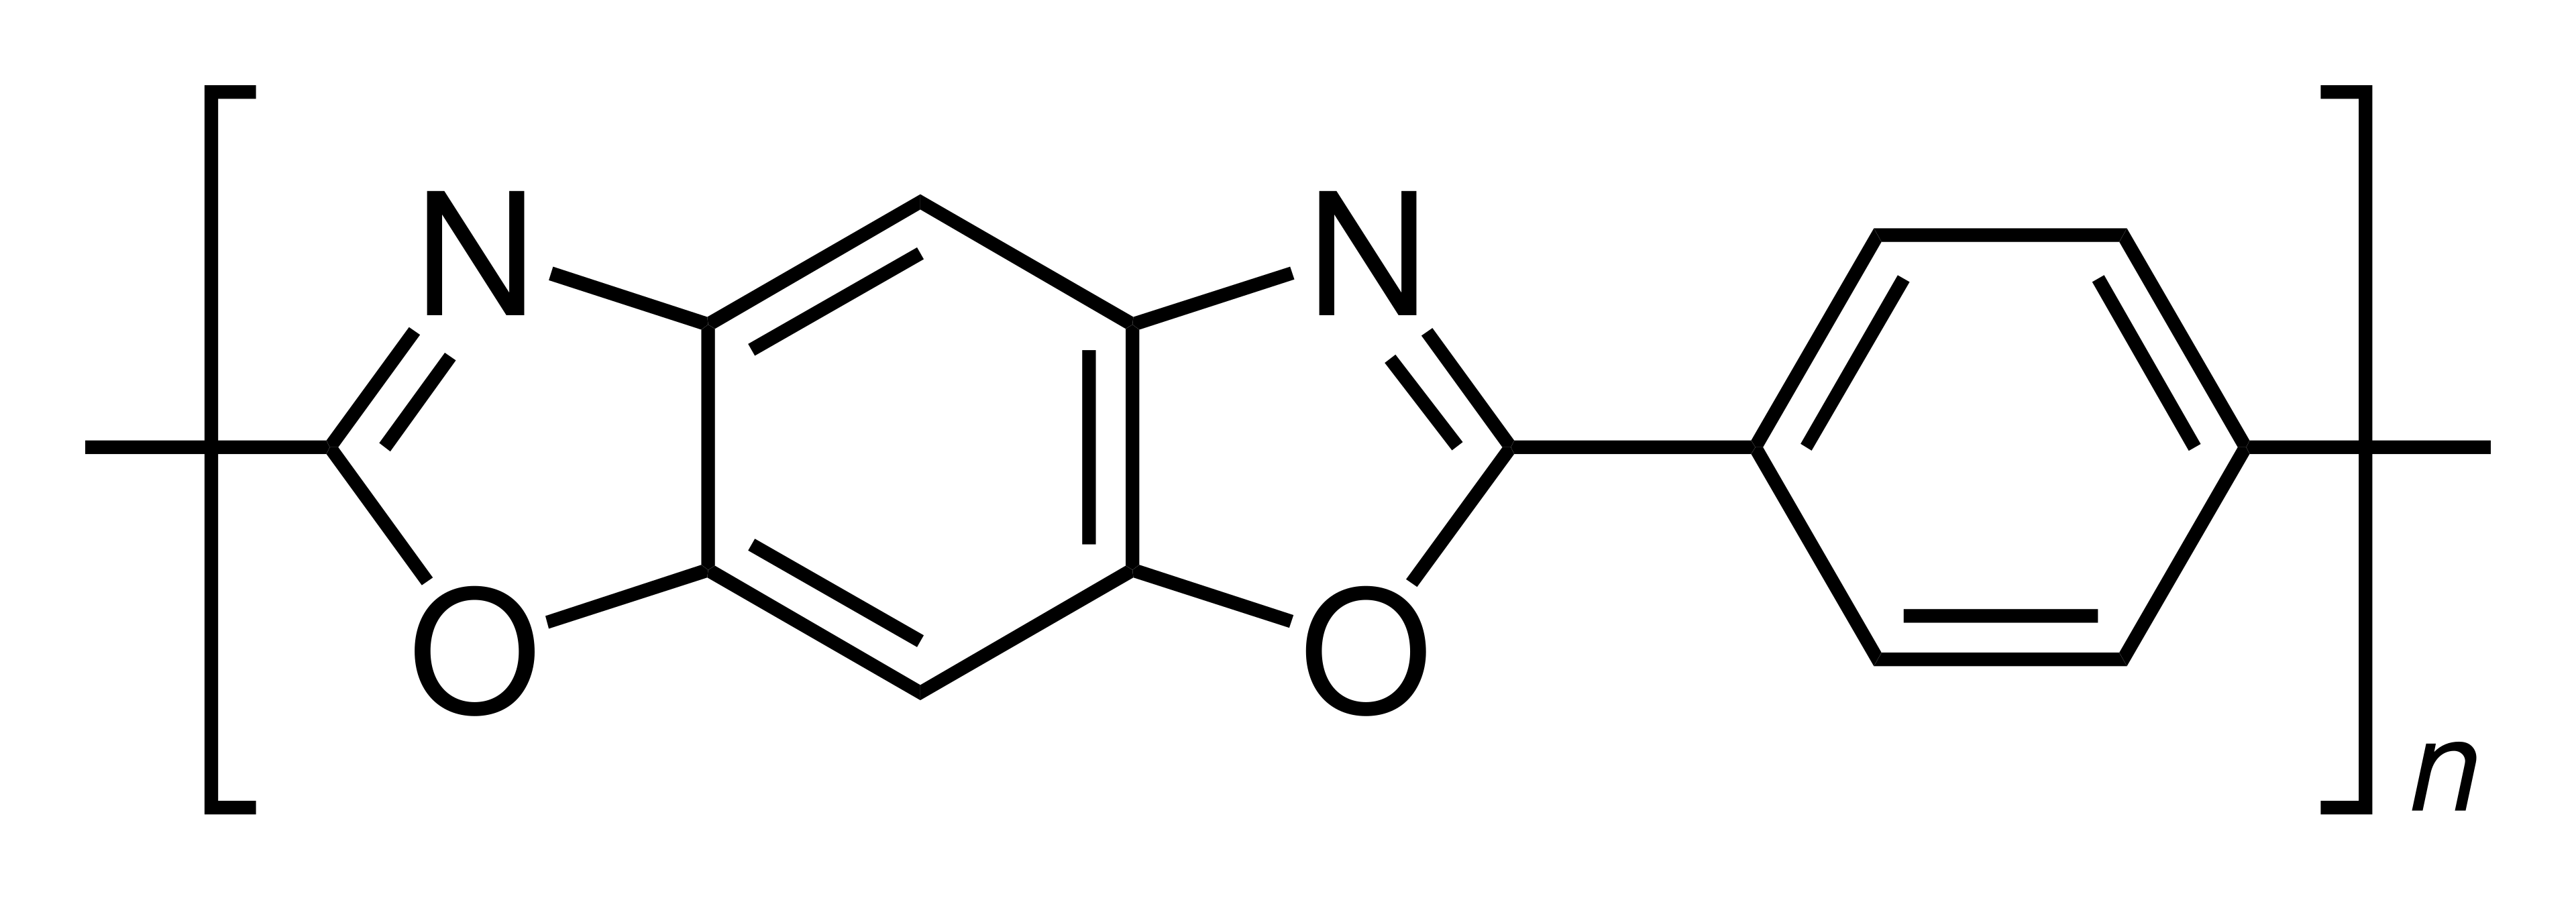
\includegraphics[width=0.5\linewidth]{fig/PBO.png}
    \caption{Molecular Structure of PBO}
    \label{fig:PBO}
\end{figure}

\noindent  At Venus middle cloud level dayside illumination, unprotected PBO would lose more than 50\% of its tensile strength within a period that is short relative to the 5-year mission. Second, technical data confirm that exposure to strong acids causes strength losses and that PBO is more stable than aramid but not immune to H$_2$SO$_4$ \cite{ZylonTechnical2005}. Third, PBO film (as opposed to the PBO fibre) remains at a low TRL for balloon applications. Foster-Miller's PIBO film work was a research-phase activity that never produced a flight-qualified balloon laminate. Fourth, the high modulus of PBO (270\,GPa) goes in parallel with a very low elongation at break (2.5\%) and is effectively brittle in the sense of being flex-fatigue sensitive, with kink-band formation at folded locations being well-documented for all rigid-rod LCP fibres \cite{VectranKinkBand}.

\medskip

\noindent For these reasons, PBO/Zylon is assessed as unsuitable as a structural load-bearing layer for the VISTA dome envelope in the absence of a fully qualified flight demonstration. It may be revisited for future missions targeting lower cloud altitudes where high-temperature capability is the primary driver.


\subsection{Polyurethane (PU) Coating}
\label{ssec:pu}

A thin polyurethane adhesive/sealant coating (Figure \ref{fig:PU}) on the inner surface of the laminate may serve as the bonding layer that binds all outer plies together and provides a thermally sealable inner surface for gore-seam construction. 

\begin{figure}[H]
    \centering
    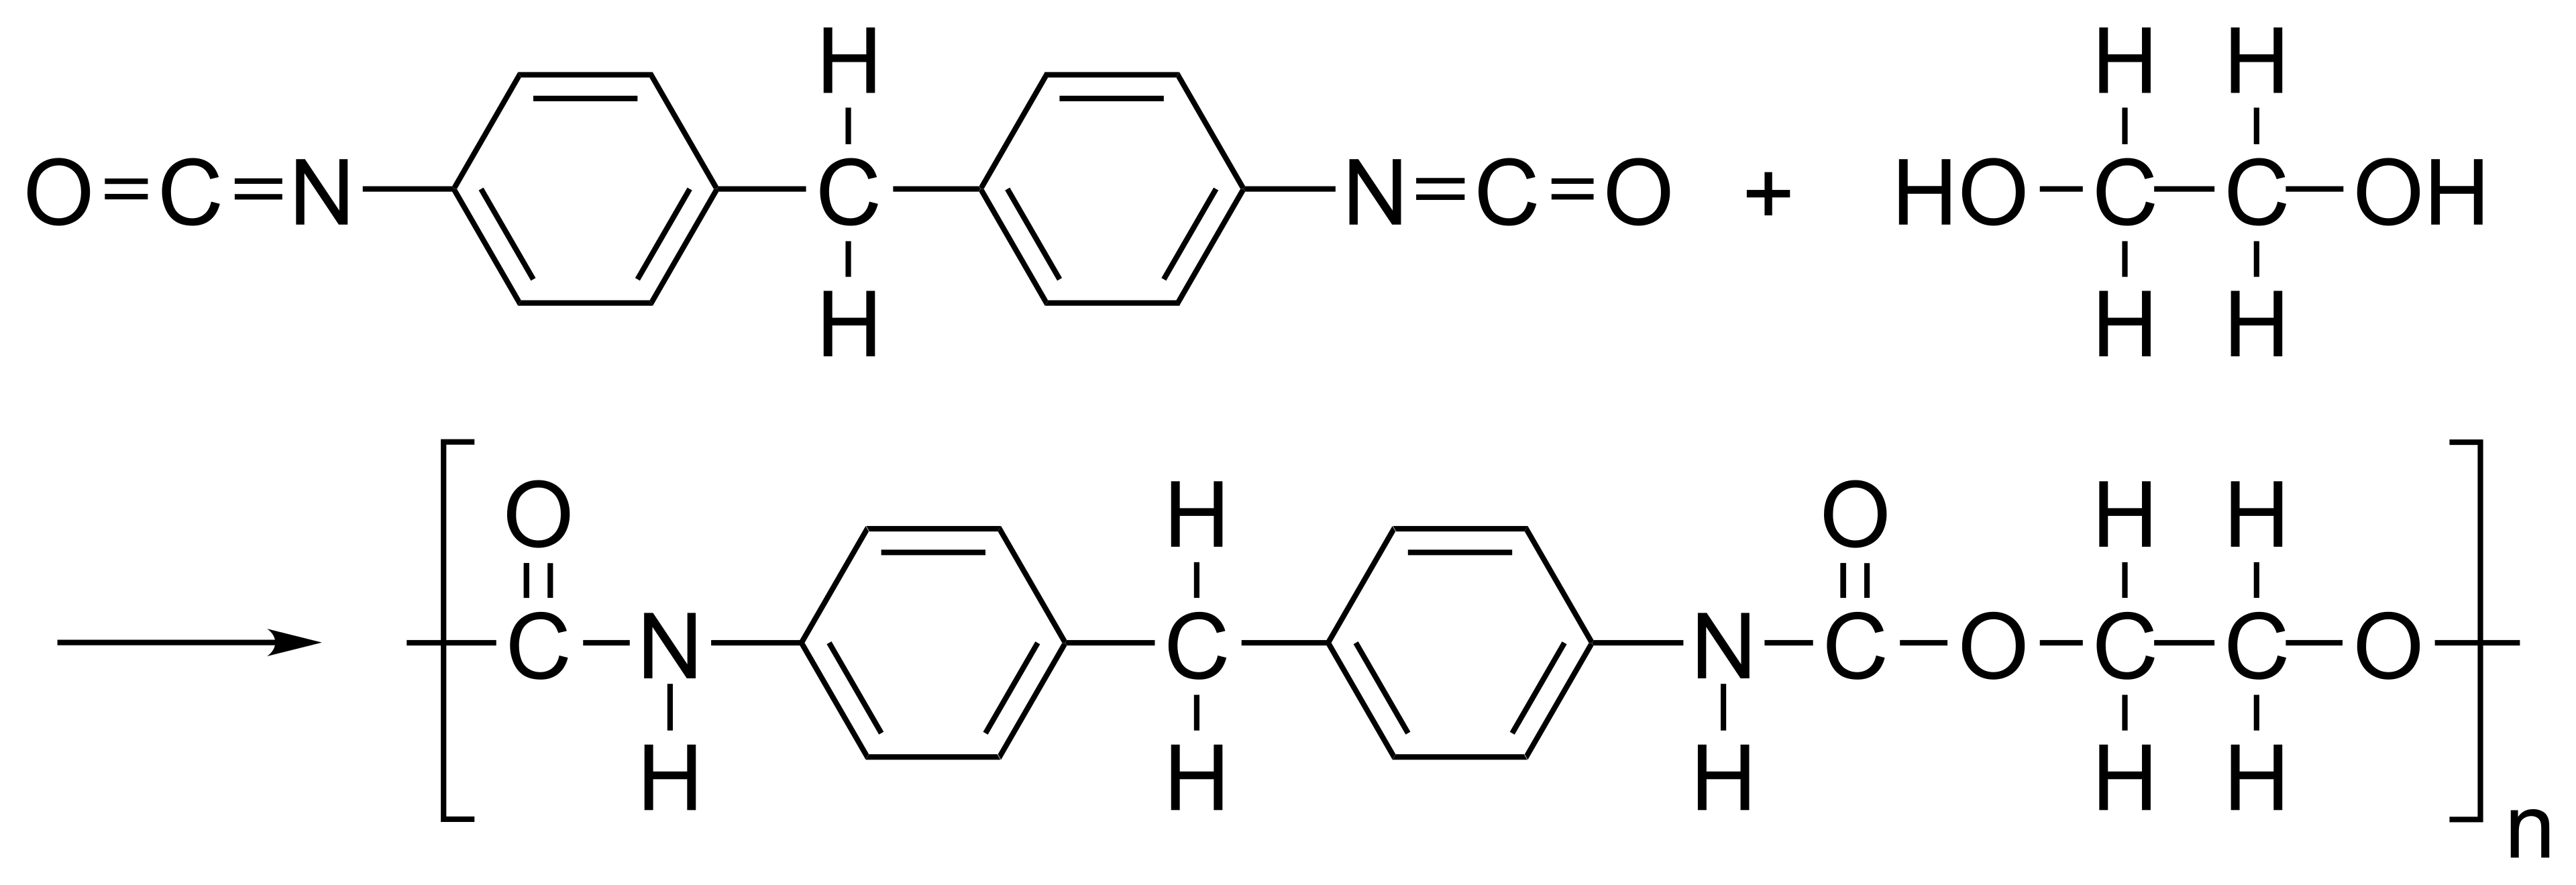
\includegraphics[width=0.7\linewidth]{fig/PU.png}
    \caption{Molecular Structure of PU}
    \label{fig:PU}
\end{figure}

In the JPL Gen-1 laminate, PU was the innermost layer \cite{Hall2007_VenusPrototype}. PU has adequate chemical resistance to nitrogen and is compatible with fabric bonding chemistry. It provides elongation and flex tolerance but contributes negligibly to gas barrier performance. Its service temperature of approximately 80-100\,$^\circ$C is adequate for the Venus cloud environment.
\fi




\section{Multi-Layer Laminate Architectures}
\label{sec:mat-architectures}

Given the individual material assessment above, no single film satisfies all material requirements simultaneously. Thus, the design space is multi-layer laminates in which distinct films perform distinct functions. Three architectures are evaluated, reflecting the evolution of JPL Venus balloon technology and VISTA-specific adaptations.


\subsection{Architecture A: JPL Gen-1 Laminate (Baseline Reference)}
\label{ssec:arch-a}

\noindent The first proposed architecture is the laminate flown in the JPL 5.5\,m diameter prototype tested in 2006 \cite{Hall2007_VenusPrototype}. The total areal density is approximately 180\,g/m$^2$. The FEP outer layer provides acid resistance and solar reflectivity via its aluminium coating. The aluminized Mylar provides gas barrier performance. The Vectran fabric provides superpressure burst strength. The polyurethane bonds and seals. This construction achieved a burst superpressure of 39\,200\,Pa and demonstrated 12 days of leak-free hold in Earth testing \cite{Hall2007_VenusPrototype}.

\bigskip

\noindent \textbf{Stack (outside to inside):}
\begin{enumerate}[parsep=0pt]
\item Aluminized FEP film (outer acid barrier and solar reflector)
\item Aluminized Mylar (PET) film (gas barrier)
\item Vectran fabric (structural)
\item Polyurethane adhesive coating
\end{enumerate}

\medskip

\noindent The known weakness of this laminate is the helium permeability of the aluminized Mylar layer: the metalised film develops pinholes during packaging and handling, and helium leaks through these pinholes, limiting float duration to weeks rather than years. This is less critical for VISTA's nitrogen-ISRU architecture because nitrogen molecules are substantially larger and permeate through pinholes more slowly, but the pinhole failure mode is still relevant for structural integrity, especially considering the long mission duration.



\subsection{Architecture B: JPL Gen-2 Laminate with Aluminium Foil}
\label{ssec:arch-b}


\noindent The second-generation JPL Venus balloon laminate was developed after the Gen-1 prototype identified FEP toughness and aluminized Mylar pinhole development as the primary failure drivers \cite{Hall2011_TechDev}. The substitution of Aclar for FEP improves outer-layer toughness and abrasion resistance. The substitution of thin aluminium foil for aluminized Mylar provides a dramatically improved gas barrier because continuous aluminium foil has no inherent polymer permeability channel, only the pinhole population, and pinhole density can be controlled by foil thickness (8-12\,µm) and lamination quality. 

\bigskip
\noindent \textbf{Stack (outside to inside):}
\begin{enumerate}[parsep=0pt]
\item Aclar (PCTFE) film (outer acid barrier)
\item Aluminium foil (gas barrier)
\item Vectran fabric (structural)
\item Polyurethane adhesive coating
\end{enumerate}

\medskip


\noindent For the VISTA nitrogen-ISRU concept, the superior gas retention of the foil layer directly reduces the steady-state nitrogen makeup demand on the ISRU subsystem, which will have a positive waterfall effect on overall performance objectives for such a long-suration mission.

\medskip

\noindent The areal density of this laminate at reference thickness is estimated at 150-170\,g/m$^2$ (depending on Vectran fabric grade and Aclar film thickness). This is at the upper edge of the nominal design case ($\sigma = 150\,\text{g/m}^2$) with a possible slight margin overlap.



\subsection{Architecture C: High-Barrier Thin-Ply Laminate}
\label{ssec:arch-c}

\noindent This architecture replaces the aluminum foil with a second PCTFE film on the inner face of the Vectran fabric, creating a symmetric polymer-only gas barrier that avoids the mechanical fragility of a metallic foil interlayer. The symmetric arrangement ensures that if the outer PCTFE film is locally damaged at a seam, the inner PCTFE film provides a secondary gas barrier. The trade-off is that the gas retention of PCTFE film is lower than that of continuous aluminium foil: PCTFE N$_2$ permeability of approximately 10\,cm$^3$/m$^2$/d/bar at 25\,µm means a measurable steady-state nitrogen flux that must be compensated by the ISRU system. However, for nitrogen (as distinct from helium), the PCTFE N$_2$ retention is expected to be improved given the ISRU replenishment capability.

\bigskip
\noindent
\begin{minipage}[t]{0.42\linewidth}
\textbf{Stack (outside to inside):}
\begin{enumerate}[parsep=0pt]
    \item Aclar (PCTFE) film (outer acid barrier)
    \item Aluminium foil (gas barrier)
    \item Vectran fabric (structural)
    \item Polyurethane adhesive coating
\end{enumerate}
\end{minipage}
\hfill
\begin{minipage}[t]{0.53\linewidth}
For the VISTA nitrogen-ISRU concept, the superior gas retention of the foil layer directly reduces the steady-state nitrogen makeup demand on the ISRU subsystem, which will have a positive waterfall effect on overall performance objectives for such a long-duration mission.
\end{minipage}

\medskip

\noindent The estimated areal density of Architecture C is approximately 140-160\,g/m$^2$, slightly lower than Architecture B if thin PFA (25\,µm) and thin PCTFE (25\,µm each face) films are used. The lower metallic mass fraction also reduces deployed stowed density, which is good for packaging.



\section{Trade-Off Analysis}
\label{sec:mat-tradeoff}

The previous section focused on search of applicable materials and as this task was completed, another stage concerns the choice of the best candidate for the mission at hand. Based on operational conditions outlined in section \ref{sec:mat-environment} and derived requirements from \ref{sec:mat-requirements}, selection criteria can be found and subsequently applied to considered materials.

\subsection{Trade-Off Criteria and Weights}
\label{ssec:tradeoff-criteria}

 The six evaluation criteria are derived directly from the material requirements in Section \ref{sec:mat-requirements}. Weights reflect the mission-critical ranking of each property for the 5-year VISTA float concept.

\begin{table}[H]
\centering
\caption{Trade-off criteria, definitions, and weights for balloon envelope material selection.}
\label{tab:tradeoff-criteria}
\footnotesize
\renewcommand{\arraystretch}{1.15}
\setlength{\tabcolsep}{4pt}
\begin{tabularx}{\linewidth}{@{}p{0.4cm} p{3cm} X p{1.0cm}@{}}
\toprule
\textbf{\#} & \textbf{Criterion} & \textbf{Definition and scoring basis} & \textbf{Weight} \\
\midrule
1 & Acid resistance & Resistance of outer layer to H$_2$SO$_4$ over 5 years; anchored to Venus-specific test data. Score 1 (fails within weeks) to 5 (no degradation, flight-proven). & 25\% \\
2 & Nitrogen gas retention & Estimated total N$_2$ leakage rate per unit area relative to ISRU replenishment capacity; lower leakage = higher score. Score 1 (exceeds ISRU budget) to 5 (minimal leakage, foil-class barrier). & 25\% \\
3 & Specific structural \newline strength & Burst-pressure capacity per unit areal mass; accounts for superpressure structural requirement. Score 1 (insufficient margin) to 5 (substantial margin at $\sigma \leq 150$\,g/m$^2$). & 20\% \\
4 & Flex and deployment tolerance & Ability to survive stowed packaging, deployment shock, and 5-year repeated thermal cycling without pinhole formation or delamination. Score 1 (brittle, pinhole risk) to 5 (no observed degradation in handling tests). & 15\% \\
5 & Long-term UV/thermal stability & Retention of strength and acid resistance under Venus UV irradiance and $\pm$20\,$^\circ$C diurnal cycling for 5 years. Score 1 (rapid photodegradation) to 5 (inherently UV-stable chemistry). & 10\% \\
6 & TRL and flight \newline heritage & Maturity level of the laminate in Venus-relevant testing. Score 1 (concept only) to 5 (flight-tested or full prototype tested at Venus conditions). & 5\% \\
\midrule
\multicolumn{3}{l}{\textit{Total}} & \textbf{100\%} \\
\bottomrule
\end{tabularx}
\end{table}



\subsection{Architecture Scoring}
\label{ssec:tradeoff-scoring}

Upon completing the list of relevant parameters to choose the best-fitting material candidate, a scoring can be assigned to each of considered designs.


\definecolor{score5}{RGB}{0,176,80}
\definecolor{score4}{RGB}{146,208,80}
\definecolor{score3}{RGB}{255,255,0}
\definecolor{score2}{RGB}{255,192,0}
\definecolor{score1}{RGB}{255,0,0}

\begin{table}[H]
\centering
\caption{Scored trade-off matrix for balloon envelope laminate architectures (score 1-5 per criterion; weighted total out of 5).}
\label{tab:tradeoff-matrix}
\footnotesize
\renewcommand{\arraystretch}{1.20}
\setlength{\tabcolsep}{4pt}
\begin{tabularx}{\linewidth}{@{}p{3.3cm}|
>{\centering\arraybackslash}p{1.8cm}|
>{\centering\arraybackslash}p{1.8cm}|
>{\centering\arraybackslash}p{1.6cm}|
>{\centering\arraybackslash}p{1.5cm}|
>{\centering\arraybackslash}p{1.2cm}|
>{\centering\arraybackslash}p{1cm}|
>{\centering\arraybackslash}p{1.3cm}@{}}
\toprule
\textbf{Architecture} &
\textbf{Acid resistance} (25\%) &
\textbf{N$_2$ retention} (25\%) &
\textbf{Sp. strength} (20\%) &
\textbf{Flex tol.} (15\%) &
\textbf{UV/ therm.} (10\%) &
\textbf{TRL} (5\%) &
\textbf{Weighted score} \\
\midrule

\textbf{A} - FEP / Al-Mylar / Vectran / PU &
\cellcolor{score4!40}4 & \cellcolor{score3!40}3 & \cellcolor{score4!40}4 & \cellcolor{score3!40}3 & \cellcolor{score4!40}4 & \cellcolor{score5!40}5 &
\textbf{3.60} \\

\textbf{B} - Aclar / Al-foil / Vectran / PU &
\cellcolor{score5!40}5 & \cellcolor{score5!40}5 & \cellcolor{score4!40}4 & \cellcolor{score4!40}4 & \cellcolor{score5!40}5 & \cellcolor{score4!40}4 &
\textbf{4.55} \\

\textbf{C} - PFA / PCTFE / Vectran / PCTFE / PU &
\cellcolor{score4!40}4 & \cellcolor{score4!40}4 & \cellcolor{score4!40}4 & \cellcolor{score5!40}5 & \cellcolor{score5!40}5 & \cellcolor{score2!40}2 &
\textbf{4.05} \\

\midrule
\multicolumn{8}{@{}p{\linewidth}@{}}{%
\textit{Notes: Scoring rationale is given in Table \ref{tab:scoring-rationale}. The acid resistance score of Architecture B outer (Aclar) is rated 5 based on Hall et al. (2011) sulfuric acid exposure test data showing no degradation of Aclar samples after prolonged immersion testing. Architecture C outer (PFA) is rated 4 because PFA has proven acid resistance at Venus conditions by chemical analogy to FEP, but has less direct Venus balloon-specific test data than Aclar. Architecture C TRL is rated 2 because the symmetric dual-PCTFE inner-face design has not been demonstrated in a Venus balloon prototype.}
} \\
\bottomrule
\end{tabularx}
\end{table}

\noindent As a means of supporting the grading shown in the Table \ref{tab:tradeoff-matrix} above, a list of rationales was compiled in the Table \ref{tab:scoring-rationale} below.

\begin{spacing}{0.95}
\begingroup
\footnotesize
\setlength{\tabcolsep}{2.5pt}
\renewcommand{\arraystretch}{1.12}
\begin{xltabular}{\linewidth}{@{}
>{\RaggedRight\arraybackslash}p{1.6cm}
>{\RaggedRight\arraybackslash}p{1.6cm}
>{\RaggedRight\arraybackslash}X
>{\centering\arraybackslash}p{0.7cm}
@{}}
\caption{Scoring rationale for the balloon envelope material trade-off.}
\label{tab:scoring-rationale} \\
\toprule
\textbf{Arch.} & \textbf{Criterion} & \textbf{Rationale and source basis} & \textbf{Score} \\
\midrule
\endfirsthead
\caption[]{Scoring rationale for the balloon envelope material trade-off. \textit{Continued from previous page.}} \\
\toprule
\textbf{Arch.} & \textbf{Criterion} & \textbf{Rationale and source basis} & \textbf{Score} \\
\midrule
\endhead
\midrule
\multicolumn{4}{r}{\textit{Continued on next page}} \\
\endfoot
\bottomrule
\endlastfoot

A & Acid resist. & FEP outer layer chemically inert to H$_2$SO$_4$ (C-F backbone); flight-proven at VEGA. Minor concern that thin aluminized-FEP surface Al may dissolve locally in prolonged acid, exposing FEP substrate, which is itself robust. Score reduced by 1 from 5 for this minor uncertainty~\cite{Hall2007_VenusPrototype,Kremnev1986}. & 4 \\
A & N$_2$ retention & Aluminized Mylar gas barrier develops pinholes during packaging; direct Gen-1 prototype leakage data showed drift after handling. N$_2$ leakage slower than He by kinetic diameter ratio, partially mitigating, but pinhole mode is non-negligible over 5 years~\cite{Hall2009_SecondGen}. & 3 \\
A & Sp. strength & Vectran fabric layer carries superpressure load; Gen-1 prototype burst at 39\,200\,Pa ($3.3\times$ worst-case)~\cite{Hall2007_VenusPrototype}. Areal density 180\,g/m$^2$ slightly above 150\,g/m$^2$ target. & 4 \\
A & Flex tol. & FEP film is prone to flex cracking relative to Aclar; aluminized Mylar develops pinholes during packaging per Gen-1 testing~\cite{Hall2009_SecondGen}. & 3 \\
A & UV/therm. & FEP inherently UV-stable (C-F); aluminium coating reflects UV from Vectran; all layers thermally stable at 35\,$^\circ$C. CTE mismatch Al/Mylar is manageable~\cite{Hall2007_VenusPrototype}. & 4 \\
A & TRL & Full 5.5\,m prototype fabricated and test-inflated; sulfuric acid coupon tests completed; leakage measured~\cite{Hall2007_VenusPrototype}. & 5 \\
\addlinespace[2pt]
B & Acid resist. & Aclar (PCTFE) outer layer: Hall et al. (2011) report no degradation in sulfuric acid exposure tests; tougher than FEP; no Al surface exposed to acid contact~\cite{Hall2011_TechDev}. & 5 \\
B & N$_2$ retention & Continuous Al foil 8-12\,µm; no intrinsic polymer permeability channel; pinhole density suppressed by lamination quality control; N$_2$ barrier dramatically superior to metallised film~\cite{Hall2011_TechDev}. & 5 \\
B & Sp. strength & Vectran fabric identical to Gen-1; areal density reduced (Aclar + Al foil lighter than FEP + Al-Mylar stack). Estimated 150-165\,g/m$^2$, at the nominal target~\cite{Hall2011_TechDev}. & 4 \\
B & Flex tol. & Aclar (elongation 100-250\%) substantially more flexible than FEP; Al foil brittle at fold lines, but in laminate the Vectran fabric constrains fold geometry; Gen-2 prototype handled without observed delamination~\cite{Hall2011_TechDev,AclarBarrierFilms}. & 4 \\
B & UV/therm. & Aclar inherently UV-stable; Al foil provides additional UV block to Vectran; CTE mismatch Al/polymer over 1825 cycles is a long-term concern not fully tested~\cite{Hall2011_TechDev}. & 5 \\
B & TRL & Aclar/Al-foil/Vectran/PU laminate samples tested in acid and optical tests; aerial deployment tested~\cite{Hall2011_TechDev}. Not full-duration 5-year test; score reduced by 1 from 5. & 4 \\
\addlinespace[2pt]
C & Acid resist. & PFA outer layer: melt-processible, fully fluorinated, proven acid resistance by analogy to PTFE/FEP; less Venus-specific test data than Aclar. Score 4~\cite{FluorocarbonPTFEvsPFA}. & 4 \\
C & N$_2$ retention & Dual PCTFE films (2$\times$25\,µm): combined N$_2$ permeability approximately 5\,cm$^3$/m$^2$/d/bar (doubled thickness halves permeance); no metallic brittleness risk; higher than Al foil but adequate for N$_2$ ISRU budget~\cite{PCTFE_Permeability_Guide}. & 4 \\
C & Sp. strength & Vectran fabric identical; total areal density estimated 140-155\,g/m$^2$; slightly lighter than B, marginally better specific strength. & 4 \\
C & Flex tol. & All-polymer laminate: no brittle metallic interlayer; PFA and PCTFE both have elongation $>$100\%; symmetric structure resists delamination under thermal cycling. No pinholes from flexing expected. Score 5~\cite{AclarBarrierFilms,FEP_PFA_permeability}. & 5 \\
C & UV/therm. & PFA and PCTFE both UV-stable; no CTE mismatch with metallic layer; polymer-only construction expected to have excellent thermal cycling fatigue life. Score 5. & 5 \\
C & TRL & Symmetric dual-PCTFE architecture not demonstrated in any Venus balloon prototype; concept only. Score 2~\cite{Hall2011_TechDev}. & 2 \\
\end{xltabular}
\endgroup
\end{spacing}


\section{Selected Architecture and Design Specification}
\label{sec:mat-selection}

Architecture B (Aclar PCTFE / Aluminium foil / Vectran fabric / Polyurethane coating, from outside to inside) is selected as the baseline VISTA balloon envelope material. It achieves the highest weighted score of 4.55/5.00, excelling on the two highest-weighted criteria (acid resistance and nitrogen gas retention). The selection is reinforced by the highest available TRL: the Aclar/Al-foil/Vectran/PU laminate has been fabricated, acid-tested, optically characterised, and aerially deployed by the JPL team \cite{Hall2011_TechDev}, making it the most mature Venus-specific balloon laminate in the open literature.

\subsection{Selection Specification}


The selected laminate specification is given in Table \ref{tab:laminate-spec}. Layer thicknesses reflect the Gen-2 prototype design reported by Hall et al. \cite{Hall2011_TechDev}, with the Vectran grade selected to match the superpressure structural requirement.

\begin{table}[H]
\centering
\caption{Selected VISTA balloon envelope laminate specification (Architecture B).}
\label{tab:laminate-spec}
\footnotesize
\renewcommand{\arraystretch}{1.18}
\setlength{\tabcolsep}{4pt}
\begin{tabularx}{\linewidth}{@{}
>{\centering\arraybackslash}p{0.5cm}
p{4cm}
p{4cm}
p{2.2cm}
p{1.5cm}
X
@{}}
\toprule
\textbf{Ply} & \textbf{Material} & \textbf{Function} & \textbf{Thick.} & \textbf{Areal mass} & \textbf{Key references} \\
\midrule
1 (out.) & Aclar PCTFE film & Acid barrier, abrasion resistance & 25\,µm & $\approx$38\,g/m$^2$ & \cite{Hall2011_TechDev,PCTFE_Permeability_Guide} \\
2 & Aluminium foil (hard-rolled) & Gas barrier (N$_2$/He) & 10\,µm & $\approx$27\,g/m$^2$ & \cite{Hall2011_TechDev} \\
3 & Vectran HS fabric, 2$\times$2 twill & Superpressure structural layer & $\approx$180\,µm & $\approx$75\,g/m$^2$ & \cite{Hall2007_VenusPrototype,VectranReview2021} \\
4 (inn.) & Polyurethane adhesive/seal coat & Bonding, seaming, inner seal & 15\,µm & $\approx$15\,g/m$^2$ & \cite{Hall2007_VenusPrototype} \\
\midrule
\multicolumn{3}{l}{\textbf{Total laminate}} & $\approx$230\,µm & $\approx$155\,g/m$^2$ & Within nominal ROM $\sigma$ case. \\
\bottomrule
\end{tabularx}
\end{table}

\noindent The total areal density of approximately 155\,g/m$^2$ is consistent with the nominal ROM envelope sizing at $\sigma = 150\,\text{g/m}^2$, with the 5\,g/m$^2$ difference within the 20\% early-phase mass margin already applied in the buoyancy calculation. The seam construction follows the bi-taped gore-seam approach of the JPL prototypes, using a sulphuric-acid-resistant adhesive on the exposed outer seam surfaces \cite{Hall2007_VenusPrototype}.



\subsection{Compliance with Material Requirements}
\label{ssec:mat-compliance}

Finally, the chosen material can be formally confronted with predefined subsystem requirements from section \ref{sec:mat-requirements}, the effect of which is shown in the Table \ref{tab:mat-compliance} below.

\begin{table}[H]
\centering
\caption{Compliance assessment of the selected laminate against material-level requirements.}
\label{tab:mat-compliance}
\footnotesize
\renewcommand{\arraystretch}{1.15}
\setlength{\tabcolsep}{4pt}
\begin{tabularx}{\linewidth}{@{}p{2.0cm} X p{1.2cm}@{}}
\toprule
\textbf{Requirement} & \textbf{Compliance evidence} & \textbf{Status} \\
\midrule
REQ-MAT-01 (acid) & Aclar outer ply: Hall et al. (2011) sulfuric acid coupon tests show no degradation; PCTFE chemistry fully inert to H$_2$SO$_4$ at 35\,$^\circ$C. & \checkmark \\
REQ-MAT-02 (N$_2$ retention) & Al foil gas barrier: continuous foil has near-zero polymer permeance; N$_2$ loss via pinholes manageable by ISRU at 15\,W steady state. & \checkmark \\
REQ-MAT-03 (tensile) & Vectran HS fabric: Gen-1 prototype burst at $3.3\times$ worst-case superpressure~\cite{Hall2007_VenusPrototype}. Safety factor $\geq$3 met. & \checkmark \\
REQ-MAT-04 (areal mass) & $\approx$155\,g/m$^2$ estimated; within 20\% mass margin of $\sigma = 150\,\text{g/m}^2$ nominal. & \checkmark \\
REQ-MAT-05 (flex) & Aclar elongation 100-250\%~\cite{AclarBarrierFilms}; Vectran fabric constrains foil fold geometry; no pinhole formation reported in Gen-2 handling tests~\cite{Hall2011_TechDev}. & \checkmark \\
REQ-MAT-06 (UV/therm.) & PCTFE and Al UV-opaque and stable; Vectran UV-sensitive but fully encapsulated; all layers thermally rated for 35\,$^\circ$C service. & \checkmark \\
REQ-MAT-07 (TRL) & Aclar/Al-foil/Vectran/PU samples: Venus acid-testing and aerial deployment completed by JPL~\cite{Hall2011_TechDev}. TRL assessed at 4-5. & \checkmark \\
\bottomrule
\end{tabularx}
\end{table}



\subsection{Residual Risks}
\label{ssec:mat-risks}

Three residual risks are identified for this material selection at the current design phase.

\begin{enumerate}
    \item \textbf{Risk 1} - Long-term CTE fatigue \\The aluminium foil (CTE $\approx$23\,ppm/K) and PCTFE film (CTE $\approx$70\,ppm/K) have a CTE mismatch of approximately 47\,ppm/K. Over 1825 diurnal cycles in thermal cycling, the accumulated shear strain at the foil-film interface will have a non-negligible impact. This is managed by the Vectran fabric, which mechanically constrains deformation, but delamination propagation from a seam edge still needs to be assessed. 
    \item \textbf{Risk 2} - Seam acid ingress \\The outer seam uses an acid-resistant adhesive, but the tape edges represent a potential ingress path for H$_2$SO$_4$ to reach aluminium foil, which is not acid-resistant. Foil corrosion would open a local gas-barrier breach. The mitigation is to lap the Aclar outer-ply edge fully over the tape \cite{Hall2011_TechDev}.
    \item \textbf{Risk 3} - Pinhole population in foil\\ Idealized pure-lattice aluminium foil has an extremely low permeability but - depending on manufacturing quality and handling - a finite pinhole population. The Gen-2 test programme at JPL did not measure the impact of these impurities quantitatively and thus a full characterisation test campaign is required before the final N$_2$ leakage rate can be confirmed.
\end{enumerate}

\noindent These shall be addressed in following design stages, as well as the planned tests to reliably confirm set assumptions and verify the stated TRL.


\section{Balloon Sizing}

\subsection*{ISRU and Balloon Architecture}

\begin{figure}[H]
    \centering
    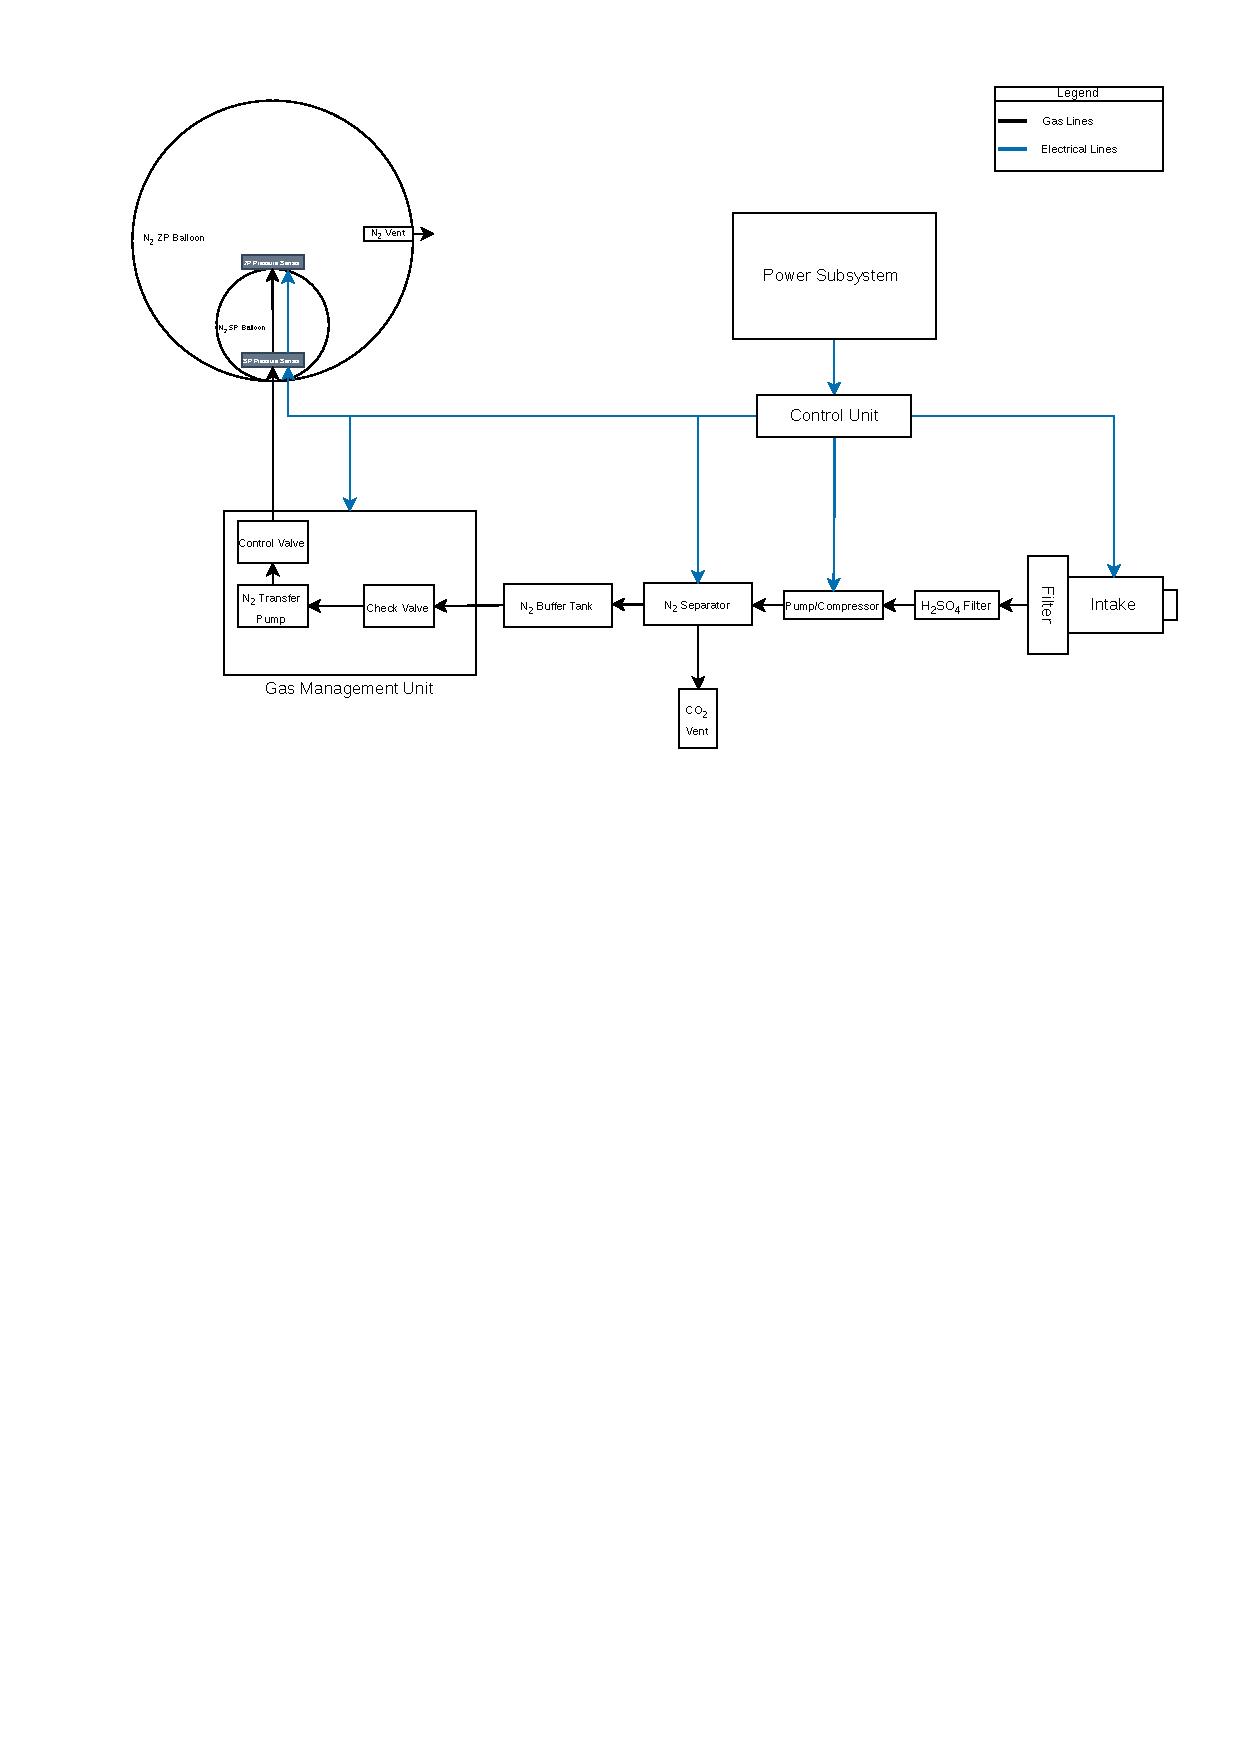
\includegraphics[draft=false,width=0.7\textwidth]{fig/ISRU_arch.pdf}
    \caption{ISRU and Balloon System}
    \label{ISRU_architecture}
\end{figure}



\begin{table}[H]
\centering
\caption{Material properties used for the balloon envelope sizing.}
\label{tab:balloon_material_properties}
\renewcommand{\arraystretch}{1.25}
\setlength{\tabcolsep}{6pt}
\begin{tabular}{l l c c c}
\hline
\textbf{Material layer} & \textbf{Main role} & 
\textbf{Thickness} & 
\textbf{Areal density} & 
\textbf{$N_2$ permeability} \\
& & 
\textbf{[$\mu$m]} & 
\textbf{[g/m$^2$]} & 
\textbf{[Barrer]} \\
\hline
Aclar PCTFE & Acid / gas barrier & 25 & 38 & 0.188~\cite{Kianfar2021} \\
Aluminium foil & Gas barrier & 10 & 27 & 0.5 \\
Vectran HS & Structural layer & 180 & 75 & $1.0 \times 10^{6}$ \\
Polyurethane (PU) & Seal / gas barrier layer & 15 & 15 & 3.25~\cite{Semsarzadeh2008PU} \\
\hline
Outer ZP envelope & Aclar + Al + PU & 50 & 80 & 0.317 \\
Inner SP envelope & Vectran HS + PU + Al & 205 & 117 & 8.328 \\ 
\hline
\end{tabular}
\end{table}

\begin{flushleft}
\footnotesize
$^{*}$ Effective permeability calculated using the series-resistance approximation \cite{Vercasson2025}:
\begin{align*}
P_{\mathrm{eff}} =
\frac{t_{\mathrm{tot}}}
{\sum_i \frac{t_i}{P_i}}
\end{align*}
where $t_i$ and $P_i$ are the thickness and nitrogen permeability of each layer.
The Vectran permeability is set to a very large value in the model, meaning that it is treated as a structural layer rather than a gas-barrier layer. The permeability value for Aluminum foil is assumed to be 0.5 \cite{Stanford1963N2O4}, in order to account for pinholes, connections and potential defects. It is a conservative, defect-adjusted effective permeability for the aluminum foil layer.
\end{flushleft}


The constants used in the code for balloon sizing are also listed in the following table:

\begin{table}[H]
\centering
\caption{Constants used in the balloon sizing model}
\label{tab:balloon_sizing_constants}
\renewcommand{\arraystretch}{1}
\begin{tabular}{l l l}
\hline
\textbf{Symbol / variable} & \textbf{Definition} & \textbf{Value} \\
\hline
$x_{N_2,\mathrm{Venus}}$ & Venus atmospheric nitrogen mole fraction & $0.035$ \\
$M_{N_2}$ & Molar mass of nitrogen & $0.0280134~\mathrm{kg/mol}$ \\
$g_{\mathrm{Venus}}$ & Venus gravitational acceleration & $8.87~\mathrm{m/s^2}$ \\
$C_D$ & Balloon drag coefficient & $0.5$ \\
$M_{\mathrm{carry}}$ & Gondola, payload, and support mass & $94~\mathrm{kg}$ \\
$\Delta p_{\mathrm{SP}}$ & Superpressure differential & $25000~\mathrm{Pa}$ \\
$D_{\mathrm{SP}}/D_{\mathrm{outer}}$ & SP-to-outer balloon diameter ratio & $0.5$ \\
$B_{\mathrm{SI}}$ & Barrer-to-SI conversion factor & $3.348\times10^{-16}~\mathrm{mol\,m/(m^2\,s\,Pa)}$ \\
$\mathrm{margin}_{\mathrm{env}}$ & Envelope mass margin & $0.15$ \\
$FS_{\mathrm{SP}}$ & Superpressure balloon factor of safety & $2.0$ \\
$\sigma_{\mathrm{Vectran,ult}}$ & Vectran ultimate tensile strength & $3\times10^9~\mathrm{Pa}$ \\
$k_{\mathrm{crimp}}$ & Crimp knockdown factor & $0.80$ \cite{Hall2021}\\
$k_{\mathrm{biaxial}}$ & Biaxial loading knockdown factor & $0.77$ \\
$k_{\mathrm{seam}}$ & Seam knockdown factor & $0.80$ \\
$k_{\mathrm{thermal}}$ & Thermal knockdown factor & $0.75$ \\
\hline
\end{tabular}
\end{table}

\subsection*{Main Assumptions}
This sizing model is preliminary, hence several assumptions are made to simplify the initial sizing approach:

\begin{enumerate}
    \item The balloon is assumed to be spherical. In reality, the balloon will have changes in curvature, seams, local wrinkling, and non-spherical deformation.
    \item The gas is assumed to behave ideally. Therefore, the gas density is calculated using the ideal gas law:
    \begin{align}
        \rho = \frac{pM}{RT}
    \end{align}
    where $\rho$ is the gas density, $p$ is the pressure, $M$ is the molar mass, $R$ is the universal gas constant, and $T$ is the temperature.
    \item The superpressure-to-zero-pressure diameter ratio is fixed at:
    \begin{align}
        \frac{D_{\mathrm{SP}}}{D_{\mathrm{ZP}}} = 0.5
    \end{align}
    This follows the preliminary balloon-in-balloon sizing assumption based on Hall et al.~\cite{Hall2021}. Since volume scales with diameter cubed, this gives:
    \begin{align}
        \frac{V_{\mathrm{SP}}}{V_{\mathrm{ZP}}} =
        \left(\frac{D_{\mathrm{SP}}}{D_{\mathrm{ZP}}}\right)^3
        = 0.5^3 = 0.125
    \end{align}
    \item The superpressure differential is fixed at:
    \begin{align}
        \Delta p_{\mathrm{SP}} = 25{,}000~\mathrm{Pa}
    \end{align}
    This is used as a representative preliminary superpressure value based on Hall et al.~\cite{Hall2021}.
\end{enumerate}
\subsection{Sizing Procedure}

The process of sizing the balloon was based on the equilibrium sizing procedure presented by Hall et al.~\cite{Hall2021}, originally developed for helium, and adapted here for nitrogen. Since the balloon is intended to operate in the Venus cloud/habitable zone, the altitude range and corresponding atmospheric properties were first defined. The model considers altitudes from $52$ to $62~\mathrm{km}$, with atmospheric temperature, pressure, and density specified at each altitude.

% Paste atmospheric data table from the code here.

Following Hall et al.~\cite{Hall2021}, a worst-case sustained vertical wind speed of 
$3~\mathrm{m/s}$ is considered for preliminary Venus aerobot sizing. The corresponding drag force is

\begin{equation}
    F_{\mathrm{drag}}
    =
    \frac{1}{2}
    \rho_{\mathrm{atm}}
    S_{\mathrm{ref}}
    v_{\mathrm{wind}}^2
    C_D ,
\end{equation}

where $\rho_{\mathrm{atm}}$, $S_{\mathrm{ref}}$, $v_{\mathrm{wind}}$ and $C_D$ are the atmospheric density, projected balloon area, vertical wind speed and drag coefficient, respectively. In the model, this is converted into an equivalent mass penalty:

\begin{equation}
    m_{\mathrm{drag}}
    =
    \frac{F_{\mathrm{drag}}}{g_{\mathrm{Venus}}}
    =
    \frac{
    \rho_{\mathrm{atm}}S_{\mathrm{ref}}v_{\mathrm{wind}}^2C_D
    }
    {2g_{\mathrm{Venus}}}.
\end{equation}
A static force balance is used to find the required outer balloon volume. The displaced atmospheric mass must balance the carried mass, envelope mass, nitrogen mass and vertical-wind drag penalty:
\begin{equation}
    \rho_{\mathrm{atm}}V_{\mathrm{outer}}
    =
    M_{\mathrm{carry}}
    +
    m_{\mathrm{env,total}}
    +
    \rho_{N_2}V_{\mathrm{ZP}}
    +
    \rho_{N_2,\mathrm{SP}}V_{\mathrm{SP}}
    +
    m_{\mathrm{drag}} .
\end{equation}
Here, $M_{\mathrm{carry}}$ is the gondola, payload and support mass, taken as $94~\mathrm{kg}$. Since the envelope and drag areas depend on the balloon volume, the equation is solved numerically for $V_{\mathrm{outer}}$ using bisection.

The SP volume is calculated from the assumed diameter ratio:
\begin{equation}
    V_{\mathrm{SP}}
    =
    \left(\frac{D_{\mathrm{SP}}}{D_{\mathrm{outer}}}\right)^3
    V_{\mathrm{outer}},
\end{equation}
and the ZP gas volume is then
\begin{equation}
    V_{\mathrm{ZP}}
    =
    V_{\mathrm{outer}} - V_{\mathrm{SP}} .
\end{equation}

Assuming spherical envelopes, the surface areas are calculated from the corresponding diameters. Using the areal densities from \autoref{tab:balloon_material_properties}, the total envelope mass is
\begin{equation}
    m_{\mathrm{env,total}}
    =
    w_{\mathrm{outer}}A_{\mathrm{outer}}
    +
    w_{\mathrm{SP}}A_{\mathrm{SP}} .
\end{equation}

The nitrogen densities are calculated using the ideal gas law. The ZP balloon is assumed to be at ambient pressure, while the SP balloon is pressurised by the imposed superpressure differential:
\begin{align}
    \rho_{N_2}
    &=
    \frac{pM_{N_2}}{RT},
    &
    \rho_{N_2,\mathrm{SP}}
    &=
    \frac{(p+\Delta p_{\mathrm{SP}})M_{N_2}}{RT}.
\end{align}
The nitrogen mass is split between the ZP and SP volumes, giving:
\begin{equation}
    m_{N_2,\mathrm{total}}
    =
    \rho_{N_2}V_{\mathrm{ZP}}
    +
    \rho_{N_2,\mathrm{SP}}V_{\mathrm{SP}} .
\end{equation}
The outer and inner envelope equivalent thicknesses are calculated from the areal density and equivalent material density:
\begin{align}
    t =
    \frac{w}{\rho_{\mathrm{mat}}}
\end{align}
Since the superpressure balloon is pressurised, its envelope experiences membrane stress. For a thin spherical pressure vessel, the membrane stress is calculated as:
\begin{align}
    \sigma_{\mathrm{SP}} =
    \frac{\Delta p_{\mathrm{SP}} r_{\mathrm{SP}}}
    {2t_{\mathrm{SP}}}
\end{align}
where $\sigma_{\mathrm{SP}}$ is the SP membrane stress, $\Delta p_{\mathrm{SP}}$ is the superpressure differential, $r_{\mathrm{SP}}$ is the SP balloon radius, and $t_{\mathrm{SP}}$ is the SP envelope thickness.

The leakage rate is estimated using a steady-state permeation model:
\begin{equation}
    \dot{n}_{N_2}
    =
    \frac{P_{\mathrm{eff}}A\Delta p_{N_2}}{t},
\end{equation}
where $P_{\mathrm{eff}}$, $A$, $\Delta p_{N_2}$ and $t$ are the effective permeability, envelope area, nitrogen partial-pressure difference and envelope thickness, respectively. For the outer envelope, the nitrogen partial-pressure difference is approximated as
\begin{equation}
    \Delta p_{N_2,\mathrm{outer}}
    =
    p(1-x_{N_2,\mathrm{Venus}}).
\end{equation}
The nitrogen replenishment rate is assumed equal to the external leakage through the outer envelope, which is converted to kg/day using
\begin{equation}
    \dot{m}_{N_2,\mathrm{day}}
    =
    \dot{n}_{N_2}M_{N_2}\cdot86400 .
\end{equation}
This calculation is repeated for each altitude and vertical wind-speed case.

A worst-case SP structural check is then performed over all altitude and wind-speed cases. Since membrane stress increases with radius, the largest SP radius is used to calculate the stress-required thickness:
\begin{equation}
    t_{\mathrm{SP,stress}}
    =
    \frac{\Delta p_{\mathrm{SP}}r_{\mathrm{SP,max}}}
    {2\sigma_{\mathrm{allow,SP}}}.
\end{equation}
The allowable SP stress is calculated using knockdown factors and a safety factor, following the approach in Hall et al.~\cite{Hall2021}:
\begin{equation}
    \sigma_{\mathrm{allow,SP}}
    =
    \frac{
    \sigma_{\mathrm{Vectran,ult}}
    k_{\mathrm{crimp}}
    k_{\mathrm{biaxial}}
    k_{\mathrm{seam}}
    k_{\mathrm{thermal}}
    }
    {FS_{\mathrm{SP}}}.
\end{equation}
The final SP design thickness is taken as
\begin{equation}
    t_{\mathrm{SP,design}}
    =
    \max\left(t_{\mathrm{SP,material}},t_{\mathrm{SP,stress}}\right).
\end{equation}
If the stress-required thickness exceeds the selected material thickness, the SP areal density is updated and the altitude/wind-speed sweep is repeated, since the increased envelope mass affects the required volume and all dependent outputs.

The results are visualised in the following plots:

% Paste the plots here.

\begin{figure}[H]
    \centering

    \begin{subfigure}{0.42\textwidth}
        \centering
        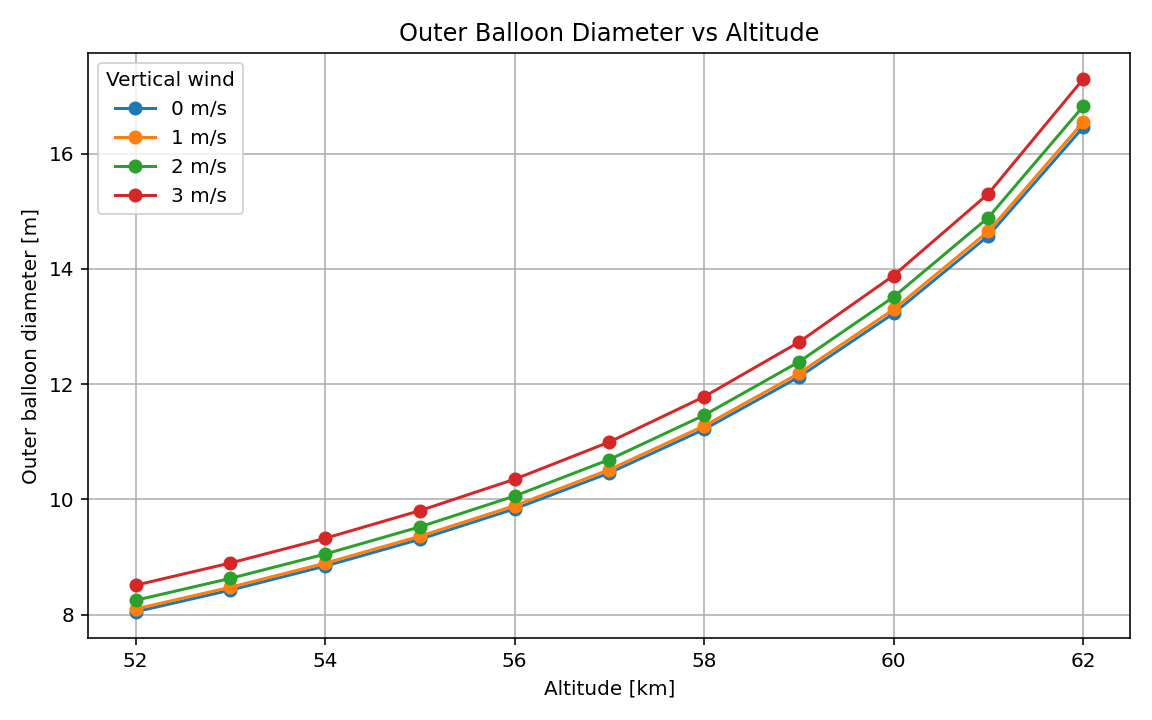
\includegraphics[width=\textwidth]{fig/Diam_plot.png}
        \caption{Outer diameter vs altitude}
        \label{fig:diameter_altitude}
    \end{subfigure}
    \hspace{0.04\textwidth}
    \begin{subfigure}{0.42\textwidth}
        \centering
        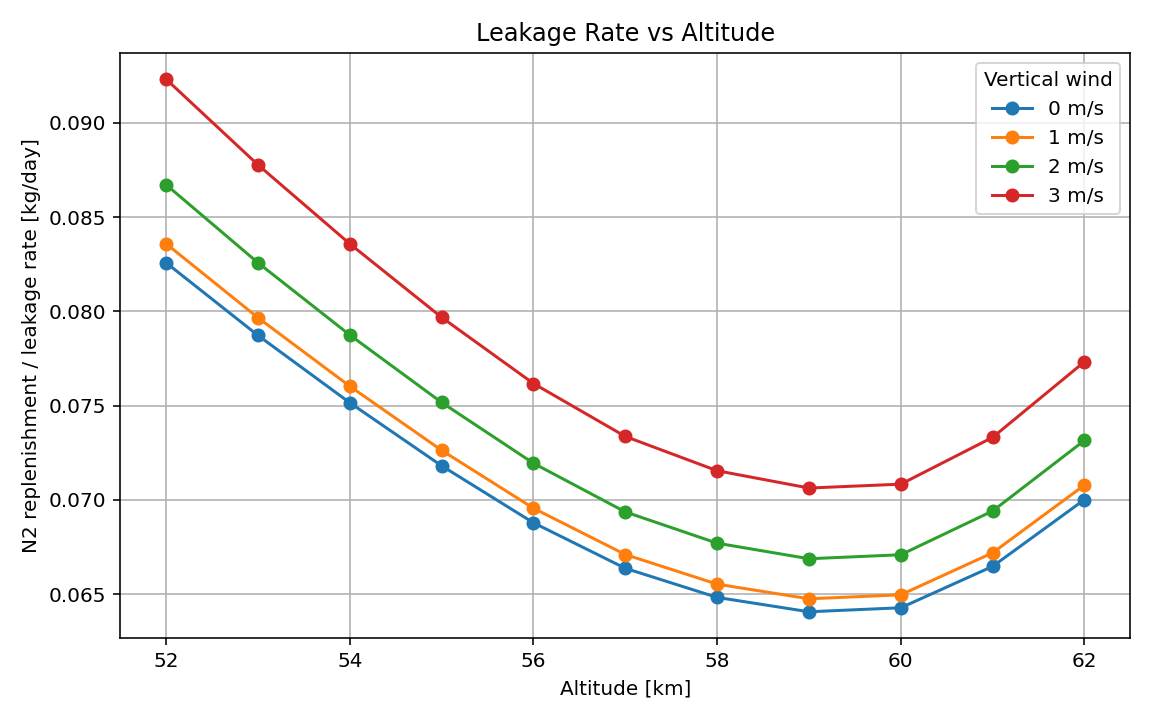
\includegraphics[width=\textwidth]{fig/Leakage_plot.png}
        \caption{N$_2$ leakage rate vs altitude}
        \label{fig:leakage_altitude}
    \end{subfigure}

    \caption{Balloon diameter and nitrogen leakage rate as a function of altitude for different vertical wind speeds.}
    \label{fig:balloon_sizing_results}
\end{figure}

Finally, the dry envelope mass of the selected configuration is calculated from the design surface areas and corresponding areal densities. A 15\% mass margin is then applied:
\begin{equation}
    m_{\mathrm{env,total,margin}}
    =
    \left(
    w_{\mathrm{outer}}A_{\mathrm{outer,design}}
    +
    w_{\mathrm{SP}}A_{\mathrm{SP,design}}
    \right)
    (1+\mathrm{margin}) .
\end{equation}
The results are summarised in the tables below. The leakage values include the applied factor-of-two sizing margin and are taken over the full altitude and vertical wind-speed sweep.

% Paste the results summary table here.

\begin{table}[H]
\centering
\caption{Envelope mass, nitrogen mass, and leakage results}
\label{tab:mass_and_leakage_results}
\renewcommand{\arraystretch}{1.08}
\small

\begin{minipage}{0.56\textwidth}
\centering
\begin{tabular}{cc@{\quad}cc}
\toprule
\multicolumn{2}{c}{\textbf{Envelope}} &
\multicolumn{2}{c}{\textbf{N$_2$ at 55 km}} \\
\cmidrule(lr){1-2} \cmidrule(lr){3-4}
$h_{\max}$ [km] & $m_{\mathrm{env}}$ [kg] &
$v_{\mathrm{wind}}$ [m/s] & $m_{N_2}$ [kg] \\
\midrule
60 & 83.83  & 0 & 264.89 \\
62 & 118.03 & 1 & 269.45 \\
   &        & 2 & 283.70 \\
   &        & 3 & 309.61 \\
\bottomrule
\end{tabular}
\end{minipage}
\hfill
\begin{minipage}{0.38\textwidth}
\centering
\begin{tabular}{lc}
\toprule
\multicolumn{2}{c}{\textbf{N$_2$ Leakage}} \\
\cmidrule(lr){1-2}
\textbf{Case} & \textbf{$\dot{m}_{N_2}$ [kg/day]} \\
\midrule
Average over sweep & 0.146 \\
Maximum over sweep & 0.185 \\
\bottomrule
\end{tabular}
\end{minipage}

\end{table}

For the rest of this report, a conservative value of 0.185 kg for the N2 flow rate will be used. It represents a maximum replenishment rate over the entire altitude-wind sweep, with a safety margin of 2.0. This margin makes sense, since the values for N2 leakage are based on an ideal membrane permeation model, and therefore do not account for manufacturing defects, degradation, pinholes etc. 





\section{ISRU Power Consumption Estimation}

As can be seen in \autoref{ISRU_architecture}, the ISRU system contains several components that consume electrical power. Some of the known values used in the power estimation are defined in Table~\ref{tab:isru_power_inputs}.

\begin{table}[H]
\centering
\caption{Fixed input values used in the ISRU power estimation}
\label{tab:isru_power_inputs}
\renewcommand{\arraystretch}{1}
\begin{tabular}{l l c}
\toprule
\textbf{Variable} & \textbf{Description} & \textbf{Value} \\
\midrule
$T_0$ & Reference separation temperature & $300~\mathrm{K}$ \cite{Hall2021} \\
$E_{\mathrm{PSA,air}}$ & PSA nitrogen specific energy for Earth air & $0.63~\mathrm{kWh/kg_{N_2}}$ \\
$x_{N_2,\mathrm{air}}$ & Nitrogen mole fraction in Earth air & $0.7808$ \\
$\gamma_{N_2}$ & Nitrogen specific heat ratio & $1.4$ \\
$\eta_{\mathrm{comp}}$ & Compressor efficiency & $0.50$ \\
$T_{\mathrm{ref}}$ & Reference compressor inlet temperature & $302.3~\mathrm{K}$ \cite{Hall2021} \\
$p_{\mathrm{ref}}$ & Reference atmospheric pressure at 55 km & $53183~\mathrm{Pa}$ \cite{Hall2021} \\
$\Delta p_{\mathrm{SP}}$ & Superpressure differential & $25000~\mathrm{Pa}$ \\
$\dot{m}_{N_2,\mathrm{transfer}}$ & Daily N$_2$ transfer between ZP and SP balloons & $15~\mathrm{kg/day}$ \\
$P_{\mathrm{valve}}$ & Rated valve power & $7.8~\mathrm{W}$ \\
$DC_{\mathrm{valve}}$ & Valve duty cycle & $0.05$ \\
$P_{\mathrm{control}}$ & Control unit power & $0.4~\mathrm{W}$ \\
$P_{\mathrm{sensor}}$ & Pressure sensor power & $0.5~\mathrm{W}$ \\
$P_{\mathrm{intake,rated}}$ & Rated intake pump power & $12 ~\mathrm{W}$ \\
$DC_{\mathrm{intake}}$ & Intake pump duty cycle & $0.5$ \\
\bottomrule
\end{tabular}
\end{table}

Values for the intake pump, nitrogen separator, and nitrogen pump for altitude control need to be calculated based on the required nitrogen replenishment rate, defined previously in Table~\ref{tab:n2_leakage_summary}. Firstly, as stated in \autoref{sec:n2_separation_tradeoff}, at this stage a PSA system is used for separating N$_2$ from CO$_2$. On Earth, the nitrogen separation energy is based on a PSA specific energy of $0.63~\mathrm{kWh/kg_{N_2}}$ \cite{Rinker2024}, which is used as a conservative baseline value. However, since the N$_2$ concentration in the Venus atmosphere is only $3.5\%$, compared to approximately $78\%$ on Earth, a correction factor is needed. For this, the ideal minimum Gibbs work of separation is used. The minimum separation work per mole of nitrogen product is calculated as \cite{Ghoniem2020}:
\begin{align}
    w_{\min}(x) =
    -RT_0
    \left[
    \ln(x)
    +
    \frac{1-x}{x}\ln(1-x)
    \right]
\end{align}
The correction factor is then defined as:
\begin{align}
    f_{\mathrm{thermal}} =
    \frac{
    w_{\min}(x_{N_2,\mathrm{Venus}})
    }
    {
    w_{\min}(x_{N_2,\mathrm{air}})
    }
\end{align}
The Venus-adjusted ISRU specific energy is therefore:
\begin{align}
    E_{\mathrm{ISRU}} =
    E_{\mathrm{PSA,air}} f_{\mathrm{thermal}}
\end{align}
The average gas-processing power of the separator is then calculated from the daily nitrogen replenishment rate as:
\begin{align}
    P_{\mathrm{gas}} =
    \frac{
    \dot{m}_{N_2,\mathrm{repl}} E_{\mathrm{ISRU}}
    }
    {24}
    \cdot 1000
\end{align}
where $\dot{m}_{N_2,\mathrm{repl}}$ is the nitrogen replenishment rate in $\mathrm{kg/day}$, $E_{\mathrm{ISRU}}$ is the Venus-adjusted specific energy in $\mathrm{kWh/kg}$, and the factor of $1000$ converts the result from kW to W.

In order to calculate the power consumption of the N$_2$ pump, which pumps nitrogen between the SP and ZP balloons and is used for altitude control, the compressor power is calculated using the standard compressor relation. First, the pressure ratio is defined as:
\begin{align}
    \Pi_c =
    \frac{P_{\mathrm{out}}}{P_{\mathrm{in}}}
    =
    \frac{p_{\mathrm{ref}}+\Delta p_{\mathrm{SP}}}
    {p_{\mathrm{ref}}}
\end{align}
where $P_{\mathrm{in}}$ is the inlet pressure and $P_{\mathrm{out}}$ is the outlet pressure. The nitrogen-specific gas constant is:
\begin{align}
    R_{\mathrm{spec},N_2} =
    \frac{R}{M_{N_2}}
\end{align}
The specific heat at constant pressure is then estimated as:
\begin{align}
    c_{p,N_2} =
    \frac{\gamma_{N_2}}{\gamma_{N_2}-1}
    R_{\mathrm{spec},N_2}
\end{align}
The compressor work per kilogram of nitrogen is estimated using \cite{NASAGlennCompressor}:
\begin{align}
    w_{\mathrm{comp}} =
    \frac{
    c_{p,N_2} T_{\mathrm{ref}}
    \left[
    \Pi_c^{\frac{\gamma_{N_2}-1}{\gamma_{N_2}}}
    -1
    \right]
    }
    {\eta_{\mathrm{comp}}}
\end{align}
where $w_{\mathrm{comp}}$ is the compressor work per kilogram, $c_{p,N_2}$ is the specific heat at constant pressure, $T_{\mathrm{ref}}$ is the reference inlet temperature, $\Pi_c$ is the pressure ratio, and $\eta_{\mathrm{comp}}$ is the compressor efficiency.

The compressor energy is converted from $\mathrm{J/kg}$ to $\mathrm{kWh/kg}$ using:
\begin{align}
    E_{\mathrm{altitude}} =
    \frac{w_{\mathrm{comp}}}{3.6\times10^6}
\end{align}
The average altitude-control power is therefore:
\begin{align}
    P_{\mathrm{altitude}} =
    \frac{
    \dot{m}_{N_2,\mathrm{transfer}}
    E_{\mathrm{altitude}}
    }
    {24}
    \cdot 1000
\end{align}
where $\dot{m}_{N_2,\mathrm{transfer}}$ is defined as $15~\mathrm{kg/day}$, which is the assumed average amount of nitrogen pumped between the SP and ZP balloons per day.

The auxiliary power includes the valves, controller, intake compressor, and two pressure sensors, located in the superpressure balloon and one inside the zero-pressure balloon, with the values defined in Table~\ref{tab:isru_power_inputs}. Finally, the total ISRU power consumption can be computed from adding all components:
\begin{align}
    P_{\mathrm{aux}} &=
    P_{\mathrm{valves}}
    +
    P_{\mathrm{control}}
    +
    P_{\mathrm{sensors}}
    \\
    P_{\mathrm{gas,final}} &=
    P_{\mathrm{gas}}
    +
    P_{\mathrm{intake}}
    \\
    P_{\mathrm{ISRU,total}} &=
    P_{\mathrm{aux}}
    +
    P_{\mathrm{gas,final}}
    +
    P_{\mathrm{altitude}}
\end{align}
The final results can be found in the table below:

% Paste final ISRU power results table here.

\begin{table}[H]
\centering
\caption{ISRU power consumption for average and maximum replenishment cases}
\label{tab:isru_power_results}
\renewcommand{\arraystretch}{1.15}
\small
\begin{tabular}{p{4.2cm} c c}
\toprule
\textbf{Case} & 
\textbf{$\dot{m}_{N_2}$ [kg/day]} & 
\textbf{$P$ [W]} \\
\midrule
Average replenishment, SF = 2.0 
& 0.146 & 45.498 \\

Maximum replenishment, SF = 2.0 
& 0.185 & 52.448 \\
\bottomrule
\end{tabular}
\end{table}

\section{Sensitivity Analysis}
A sensitivity analysis has been performed for both the balloon sizing and ISRU power consumption estimation, in order to identify the parameters that affect the design the most. For the balloon sizing model, the most sensitive parameter is the maximum operating altitude. At 62 km altitude, the atmospheric density requires a larger envelope, pushing the envelope mass to 118 kg, including the safety margin, which exceeds the 100 kg requirement. On the other hand, if the maximum operating altitude is decreased to 60 km, the envelope mass becomes 76 kg, including margin, which makes the design compliant with the envelope mass requirement.
Some other important parameters include the gondola mass, envelope areal density, superpressure and permeability. An increase in the gondola mass directly increases the required balloon volume and the mass of nitrogen gas. A decrease in envelope areal density reduces the envelope mass. Superpressure mainly affects the power used by the compressor that pumps N2 between the superpressure and zero-pressure balloons, as well as the nitrogen mass and structural margin.
\newline
In the power estimation model for ISRU, the parameters that affect power consumption the most are the N2 replenishment rate and the assumed separation energy. A change in gas replenishment rate affects the power consumption almost linearly, as more leaked nitrogen requires more nitrogen to be separated each day. The required separator power is also important, as it defines how much power is required to produce a kilogram of N2 from the Venus atmosphere.
Altitude control is directly affected by the amount of N2 transferred between the superpressure and zero-pressure balloons, as a higher transfer rate or a higher pressure increase the power consumption.

\section*{Verification and Validation}
Verification and validation have been performed for both the balloon sizing and ISRU power consumption estimation.
For verification, the main method used was analysis, together with inspection of the equations used in the model and the code outputs. The balloon sizing model was checked against the altitude range, envelope mass, structural sizing and leakage requirements.
The aerobot is able to operate within the atmospheric pressure range, as well as the atmospheric temperature range, therefore supporting REQ-C-ENV-01 and REQ-C-ENV-02 \cite{baseline_vista}. On the other hand, for a maximum altitude of 62 km, the required mass of the envelope is 118 kg, which is not compliant with REQ-C-SUB-02, which limits the envelope mass to 100 kg. However, if the maximum altitude is decreased to 60 km, the envelope mass drops to 76 kg, which makes the design compliant.
The superpressure balloon design was verified by comparing the required thickness calculated from the pressurised sphere formula with the material architecture thickness of the selected material combination. The leakage rate was verified by checking the permeability conversion and confirming that the leakage scales correctly with zero-pressure envelope area, pressure difference and thickness. The resulting N2 replenishment rate was then used as an input to the ISRU power estimation model.
\newline
The ISRU power estimation model was verified by checking the energy conversion from kWh/kg to average power, and by separating the main power components into auxiliary power, gas processing power and altitude-control power. This helps verify that the model accounts for the main power-consuming elements. The power result should later be verified against the final power and energy storage requirement, once the complete subsystem power budget is fixed.
\newline
Both models are still at a preliminary stage. They are validated against existing aerobot studies in terms of static force equilibrium, SP/ZP volume behavior, ideal gas assumptions and pressure-based altitude-control logic. However, the models are not yet fully validated for mission performance, as they do not include long-term material degradation, seam leakage, corrosion damage, damage during manufacturing or clogging. These effects are particularly important for REQ-F-ENV-03 \cite{baseline_vista}. Therefore, further validation should include material exposure testing in representative Venus cloud conditions, permeability testing of the final laminate including seams, inspection of manufacturing defects, and clogging tests for the ISRU intake and separator.

\chapter{Communication and Data Handling}
\label{chap:comms}
%more detail: add exact system noise temperature calculation

\section{Space Mission Architecture and Downflowing Requirements}
%mission architecture
The communication architecture consists of three main elements: the aerobot in the Venus cloud layer, the Venus orbiter, and the ESTRACK ground station on Earth. The aerobot collects science and housekeeping data and sends it to the orbiter through a short-range relay link. The orbiter then stores and forwards the data to Earth using a deep-space communication link.

The same relay architecture is used for command uplink in the opposite direction: commands are sent from Earth to the orbiter and then relayed to the aerobot for mode updates, sampling changes, data-handling updates, and contingency operations. Direct aerobot--Earth communication is not selected, because the large Earth--Venus distance would require transmitter power, antenna gain, and pointing accuracy that are not practical for a balloon-borne gondola.

%requirements 
\medskip
\noindent A set of top-level communication requirements is defined in Table~\ref{tab:communication_requirements}. 
% These requirements are used to guide the communication system trade-off and to ensure that both the aerobot-orbiter relay link and the orbiter-Earth deep-space link satisfy the mission needs.

\begin{table}[H]
    \centering
    \small
    \caption{Top-level communication requirements.}
    \label{tab:communication_requirements}
    \begin{tabular}{p{0.13\textwidth} p{0.33\textwidth} p{0.44\textwidth}}
        \hline
        \textbf{ID} & \textbf{Requirement} & \textbf{Rationale} \\
        \hline
        REQ-COM-01 & 
        The bit error rate of the data received on Earth shall not exceed 
        $1 \times 10^{-6}$. & 
        This value is selected in accordance with ITU recommendations for 
        unmanned deep-space research missions~\cite{ITU-R-SA1014-4-2023}. \\
        \hline
        REQ-COM-02 & 
        The communication link from the aerobot to the orbiter shall support a useful data rate of at least $1500~\mathrm{bit/s}$. & 
        This requirement is derived mission description \\
        \hline
        REQ-COM-03 & 
        The communication link between the orbiter and Earth shall be compatible with the ESTRACK ground-station network. & 
        Compatibility with ESTRACK constrains the selection of frequency band, modulation, coding, antenna gain, and operational link budget. \\
        \hline
        REQ-COM-04 &
        Each communication link shall close with a positive link margin under worst-case mission geometry. &
        This ensures reliable communication at maximum range, including losses due to free-space propagation, atmosphere, pointing, polarization mismatch, and implementation losses. \\
        \hline
        REQ-COM-05 & The antenna shall maintain a communication link with the orbiter for >90\% of the time whenever the orbiter is above the local horizon & Maintaining communication over the visibility window maximizes the available time for data transmission and reduces the risk of data loss. NASA/JPL’s DESCANSO link design material states that historical deep-space RF links have achieved an overall link availability of about 90\%  \cite{chen2006linkSystemDesign} \\
        \hline
    \end{tabular}
\end{table}


\section{Frequency band selection}
The frequency band selection is a key design driver because it affects achievable data rate, antenna gain, transmitter power, link margin, propagation losses, ground-station compatibility, and frequency-allocation constraints. For the orbiter--Earth link, the main ESTRACK-compatible deep-space options are S-band, X-band, and Ka-band, as summarized in \autoref{tab:estrack_frequency_bands}. X-band is selected as the baseline because it provides the best compromise between reliability, data-rate capability, antenna size, and ESTRACK compatibility. Compared with S-band, it offers higher bandwidth and higher antenna gain for a given antenna size; compared with Ka-band, it is less sensitive to atmospheric attenuation, rain losses, and pointing errors, making it more robust for a relatively low-data-rate Venus mission.

\begin{table}[H]
    \centering
    \small
    \caption{Candidate ESTRACK-compatible frequency bands for the orbiter--Earth link.}
    \label{tab:estrack_frequency_bands}
    \begin{tabular}{p{0.22\textwidth} p{0.34\textwidth} p{0.34\textwidth}}
        \hline
        \textbf{Band} & \textbf{Uplink: Earth to orbiter} & \textbf{Downlink: orbiter to Earth} \\
        \hline
        S-band & $2110$--$2120~\mathrm{MHz}$ & $2290$--$2300~\mathrm{MHz}$ \\
        \hline
        X-band & $7145$--$7190~\mathrm{MHz}$ & $8400$--$8450~\mathrm{MHz}$ \\
        \hline
        Ka-band & $34.2$--$34.7~\mathrm{GHz}$ & $31.8$--$32.3~\mathrm{GHz}$ \\
        \hline
    \end{tabular}
\end{table}

For the aerobot--orbiter relay link, direct use of X-, S-, or Ka-band is less attractive because the balloon gondola has limited pointing capability and power. The candidate proximity-link bands are therefore VHF, UHF, and S-band, as shown in \autoref{tab:aerobot_orbiter_frequency_bands}. VHF has low path loss and is robust, but requires larger antennas and has less modern planetary relay heritage. S-band is possible, but has higher path loss and generally requires better antenna gain or pointing. UHF is selected as the baseline because it is well suited to short-range planetary relay, low data rates, low spacecraft complexity, broad antenna coverage, and weak pointing requirements.

\begin{table}[H]
    \centering
    \small
    \caption{Candidate frequency bands for the aerobot--orbiter communication link.}
    \label{tab:aerobot_orbiter_frequency_bands}
    \begin{tabular}{p{0.30\textwidth} p{0.50\textwidth}}
        \hline
        \textbf{Band} & \textbf{Frequency range} \\
        \hline
        VHF & $30$--$300~\mathrm{MHz}$ \\
        \hline
        UHF & $300~\mathrm{MHz}$--$3~\mathrm{GHz}$ \\
        \hline
        S-band & $2$--$4~\mathrm{GHz}$ \\
        \hline
    \end{tabular}
\end{table}

\section{Link Analysis}
\subsection{Modulation, Coding and Spectral Efficiency}
Based on the modulation trade-off in \autoref{tab:modulation_tradeoff}, the most suitable schemes for the aerobot--orbiter UHF link are BPSK, MSK/GMSK, and QPSK. Since the required data rate is low, robustness and power efficiency are more important than spectral efficiency. BPSK is power-efficient and requires a low \(E_b/N_0\), reducing transmitter power, but it requires coherent carrier recovery and is therefore sensitive to Doppler, oscillator stability, and phase tracking. MSK/GMSK is retained as the main alternative because its constant-envelope waveform allows efficient nonlinear power amplification and good spectral containment. QPSK is possible, but its higher spectral efficiency is not necessary for this low-rate link, while FSK and higher-order PSK/QAM schemes are rejected due to lower power efficiency or higher sensitivity to noise, phase errors, and amplifier nonlinearities.

\begin{table}[H]
    \centering
    \small
    \caption{Comparison of candidate modulation schemes}
    \label{tab:modulation_tradeoff}
    \begin{tabularx}{\textwidth}{p{0.18\textwidth} X X}
        \toprule
        \textbf{Modulation} & \textbf{Main advantage} & \textbf{Main disadvantage} \\
        \midrule
        Noncoherent BFSK & Simple and robust acquisition without coherent carrier recovery. & Higher required \(E_b/N_0\) and larger bandwidth than BPSK. \\
        \midrule
        Coherent BFSK & More energy-efficient than noncoherent BFSK. & Still less efficient than BPSK and requires coherent reception. \\
        \midrule
        BPSK & Very power-efficient and robust for low-rate links. & Requires coherent carrier recovery and phase tracking. \\
        \midrule
        MSK/GMSK & Constant-envelope waveform enables efficient power amplification and good spectral containment. & Slightly more complex than simple FSK and requires compatible modem implementation. \\
        \midrule
        QPSK & Higher spectral efficiency than BPSK with similar ideal \(E_b/N_0\) performance. & Extra spectral efficiency is not needed and phase recovery is more complex. \\
        \midrule
        8-PSK / 16-PSK & Higher spectral efficiency. & Requires higher \(E_b/N_0\) and is more sensitive to phase noise and nonlinearities. \\
        \midrule
        16-QAM & High spectral efficiency using amplitude and phase. & Requires high SNR, accurate amplitude/phase tracking, and a linear power amplifier. \\
        \bottomrule
    \end{tabularx}
\end{table}

\begin{figure}[H]
    \centering

    \begin{minipage}[t]{0.48\textwidth}
        \vspace{0pt}
        \small
        Channel coding is included to improve link reliability by adding redundancy, allowing the receiver to detect and correct bit errors after demodulation. This reduces the required \(E_b/N_0\) for a given BER and is included in the link budget as coding gain, at the cost of transmitting additional non-information bits. Candidate schemes include convolutional coding with Viterbi decoding, Turbo coding, and LDPC coding, with approximate coding gains shown in \autoref{fig:coding-gains}. For the aerobot--orbiter link, decoding is mainly performed on the orbiter. Pulse shaping is defined by the raised-cosine roll-off factor, which reduces intersymbol interference but increases occupied bandwidth.
    \end{minipage}
    \hfill
    \begin{minipage}[t]{0.48\textwidth}
        \vspace{0pt}
        \centering
        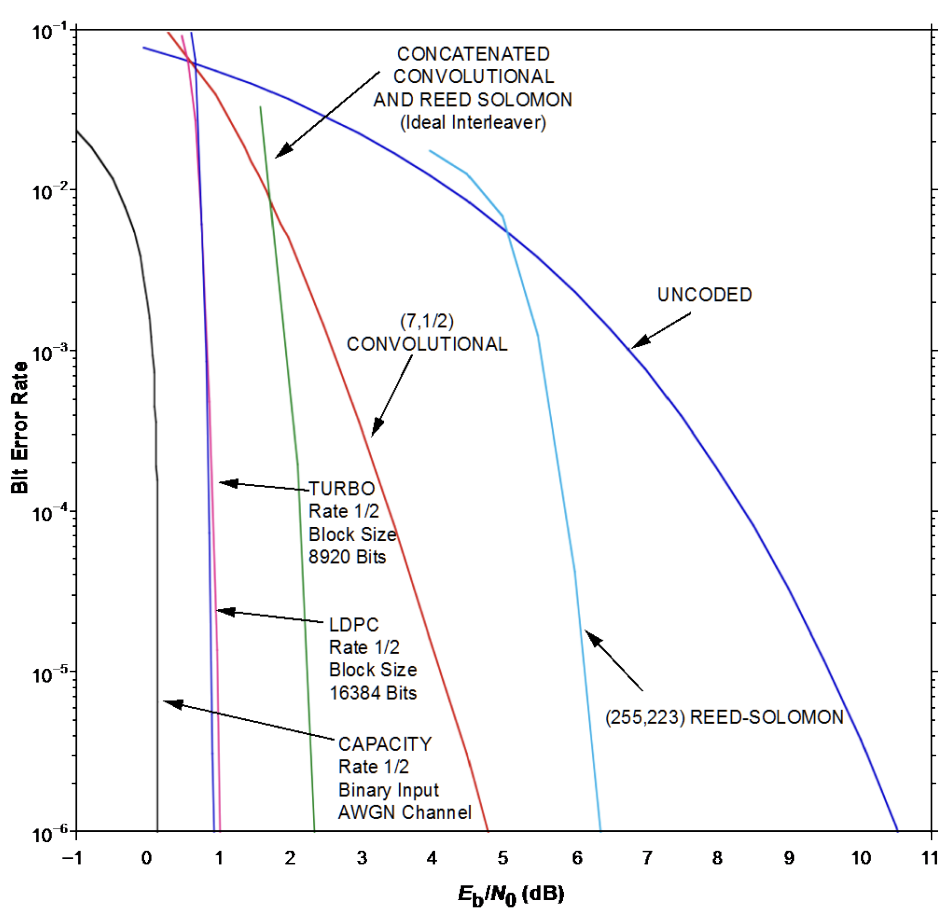
\includegraphics[width=\linewidth]{fig/Coding gains.png}
        \caption{Performance comparison of selected convolutional, Reed--Solomon, concatenated, LDPC, and Turbo codes \cite{ccsds2020_tm_sync_channel_coding}.}
        \label{fig:coding-gains}
    \end{minipage}

\end{figure}
\subsection{Propagation losses}
The simplest source of propagation loss is the free-space path loss, which represents the spreading loss of an electromagnetic wave as it propagates through space. It is given by \autoref{eq:space-loss}

\begin{equation}
    L_{fs} = 20 \log_{10}\left(\frac{4 \pi d}{\lambda}\right)
    \label{eq:space-loss}
\end{equation}

\noindent where $L_{fs}$ is the free-space path loss in dB, $d$ is the distance between the transmitter and receiver, and $\lambda$ is the signal wavelength.

\medskip
\noindent The second source of signal loss is absorption by atmospheric gases. The atmosphere of Venus consists of approximately 96.5\% $CO_2$ and 3.5\% $N_2$. \autoref{fig:absorption-rates} shows the absorption rates, expressed in dB/km, of several gases in the Venusian atmosphere for X-band and S-band frequencies. The figure also shows that below altitudes of approximately 50 km, the abundance of $H_2SO_4$ becomes significant, extending down to about 30 km. At lower frequencies, such as those in the UHF range, these absorption rates are expected to be even lower.

\begin{figure}[H]
    \centering

    \begin{minipage}{0.48\textwidth}
        \centering
        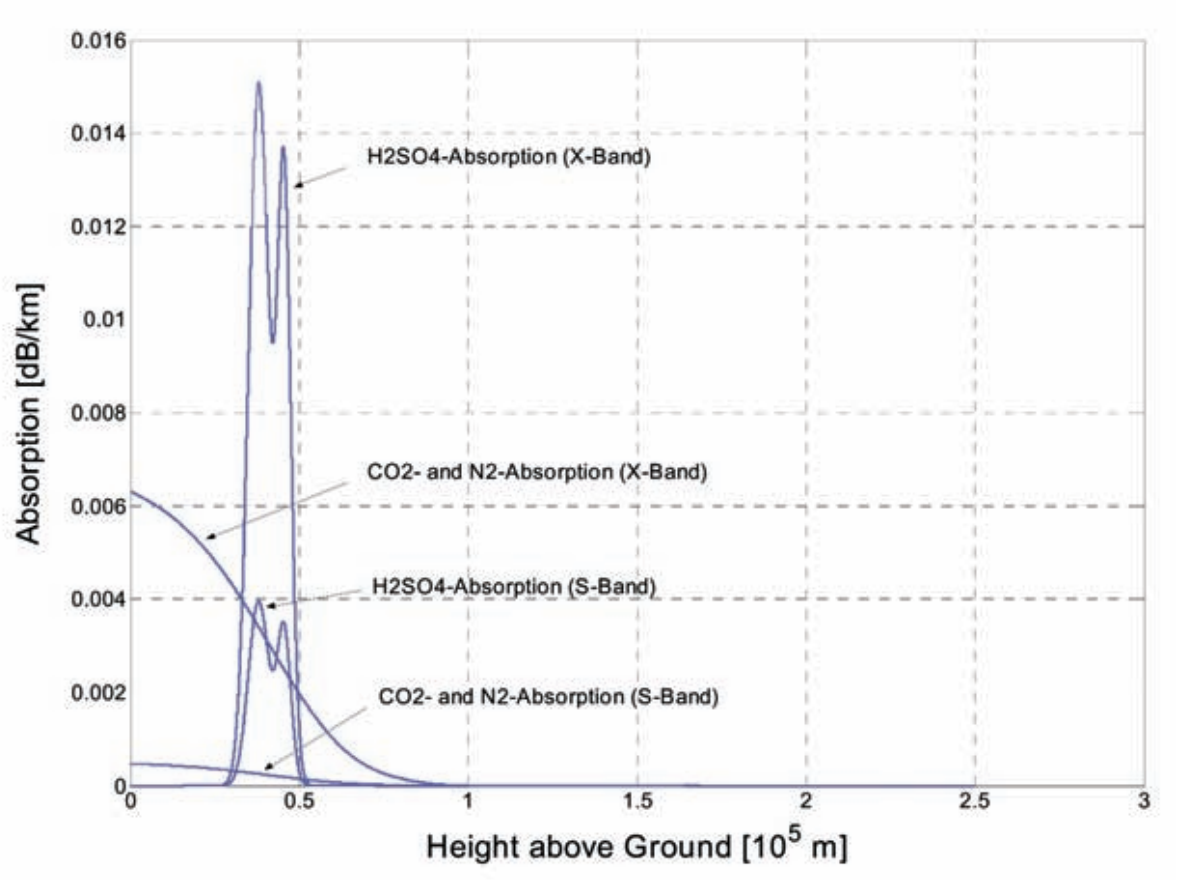
\includegraphics[width=\linewidth]{fig/Radio absorption Venus Atmosphere gasses.png}
        \caption{Average absorption profile as a function of altitude for $H_2SO_4(g)$, $CO_2$, and $N_2$ in the atmosphere of Venus \cite{hausler2007vera}.}
        \label{fig:absorption-rates}
    \end{minipage}
    \hfill
    \begin{minipage}{0.48\textwidth}
        \centering
        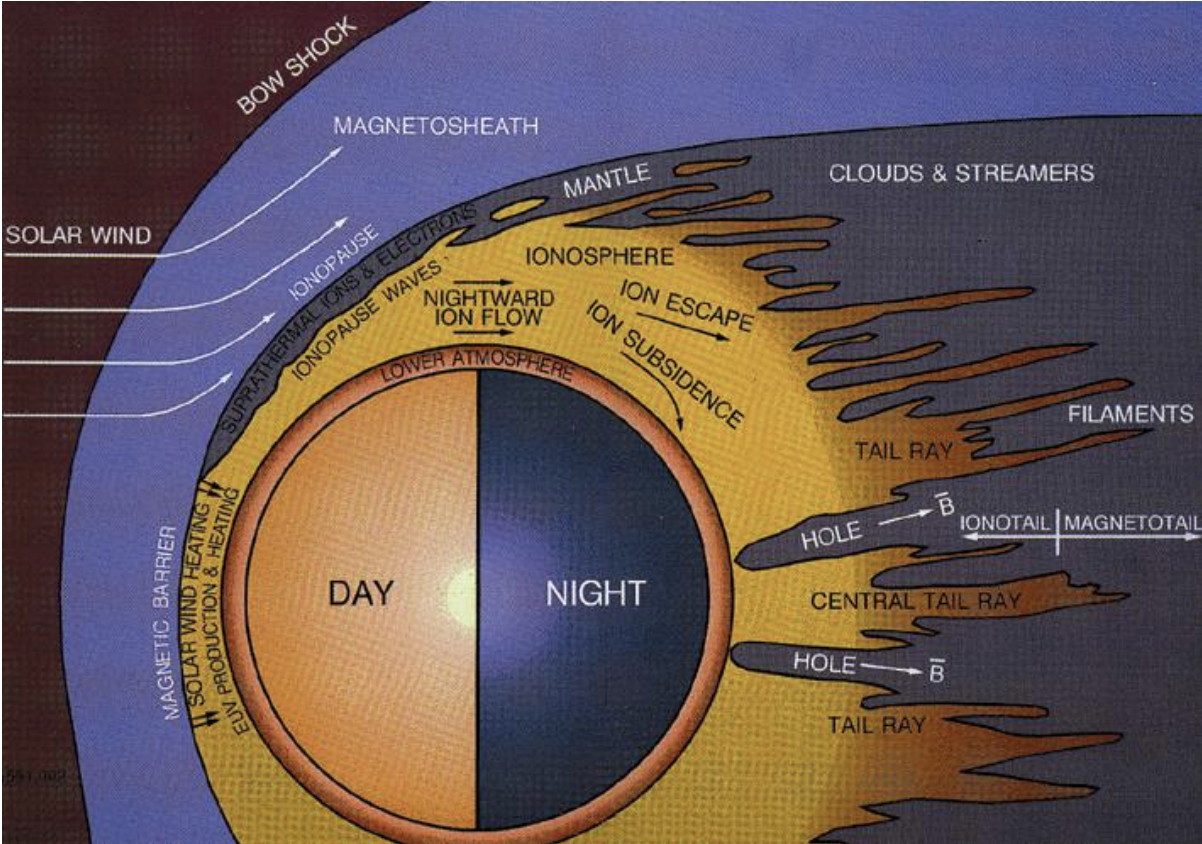
\includegraphics[width=\linewidth]{fig/Ionosphere.png}
        \caption{A sketch of the most important plasma boundaries and interaction regions in the environment of Venus \cite{angsmann2011magnetic}.}
        \label{fig:ionosphere illustation}
    \end{minipage}

\end{figure}

The Venus ionosphere is dynamic because electron density varies with altitude, solar illumination, solar activity, and solar-wind conditions. Since Venus lacks a strong intrinsic magnetic field, its plasma environment is mainly shaped by interaction with the solar wind, forming an induced magnetosphere as illustrated in \autoref{fig:ionosphere illustation}. These variations can affect UHF propagation between the aerobot and orbiter and are therefore included in the link-budget loss model.

% \autoref{fig:electron-density} shows the variation of electron density with time and solar zenith angle. 
For the link budget, a conservative case is used by taking the maximum electron-density envelope and the highest ionopause condition. The ionospheric absorption loss is calculated as
\begin{equation}
L_{\mathrm{ion,abs}} =
\frac{1.17 \times 10^{-6}\,\nu\,\mathrm{TEC}}
{n_{\mathrm{re}} f^2}
\label{eq:ionosphere-absorption}
\end{equation}
where \(L_{\mathrm{ion,abs}}\) is the absorption loss in dB, \(\nu\) is the effective electron collision frequency, \(f\) is the signal frequency, and \(n_{\mathrm{re}}\) is the real part of the plasma refractive index. For UHF, \(n_{\mathrm{re}}\approx 1\), since the signal frequency is much larger than the local plasma frequency.

% \begin{figure}[ht]
%     \centering

%     \begin{subfigure}[t]{0.48\linewidth}
%         \centering
%         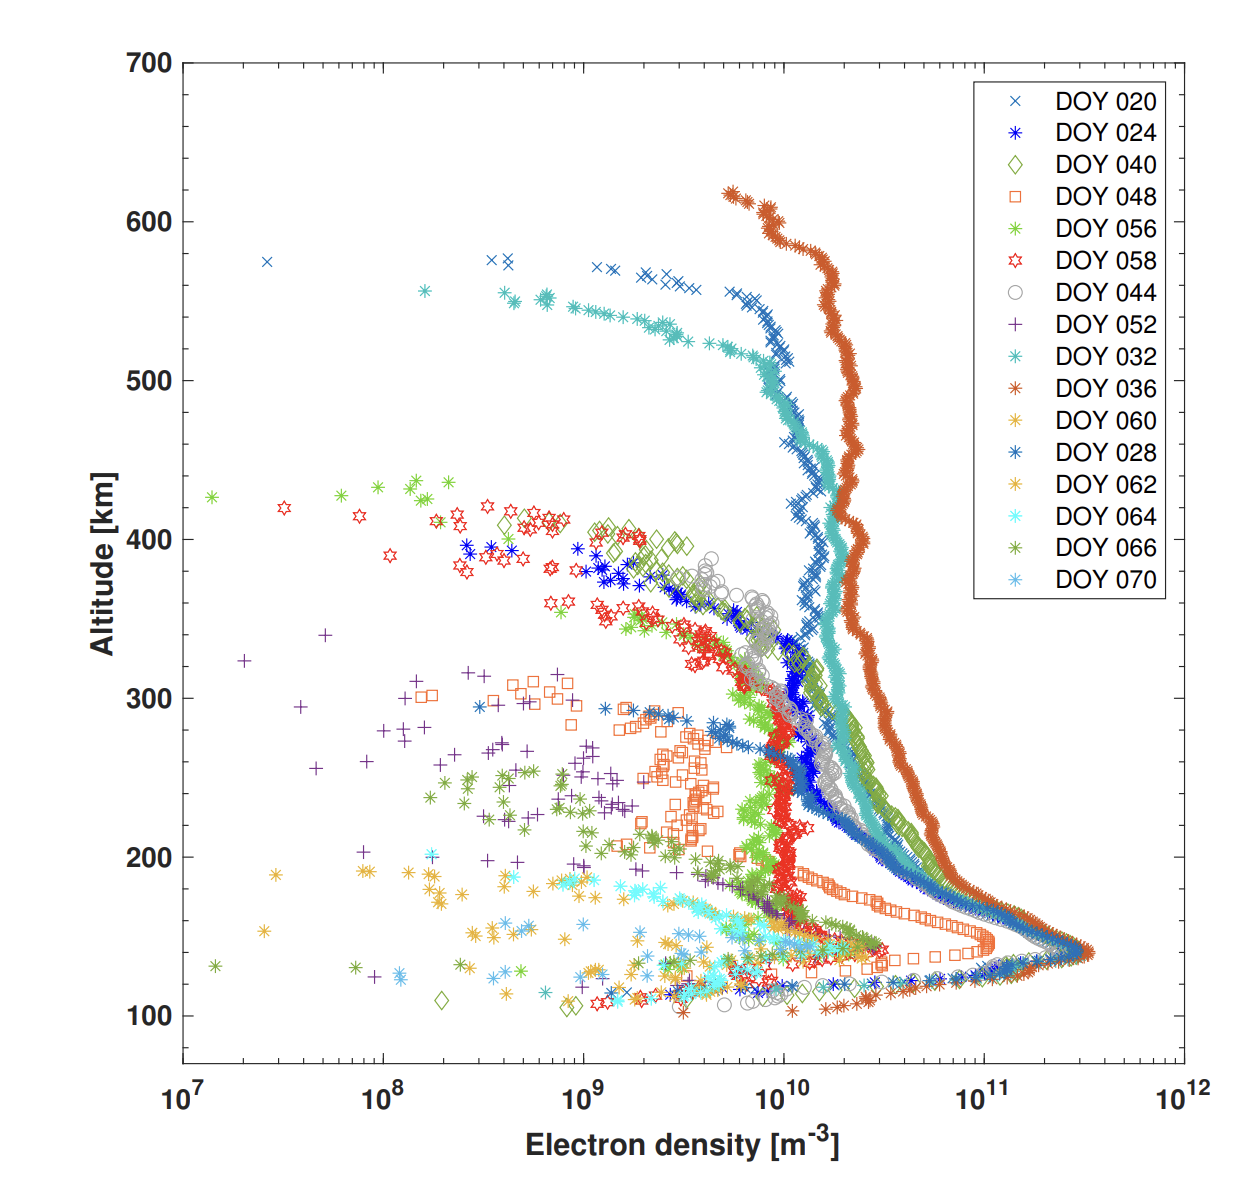
\includegraphics[width=\linewidth]{fig/Electron density different moments.png}
%         \caption{Electron density measured at different time instances}
%         \label{fig:electron-density-1}
%     \end{subfigure}
%     \hfill
%     \begin{subfigure}[t]{0.48\linewidth}
%         \centering
%         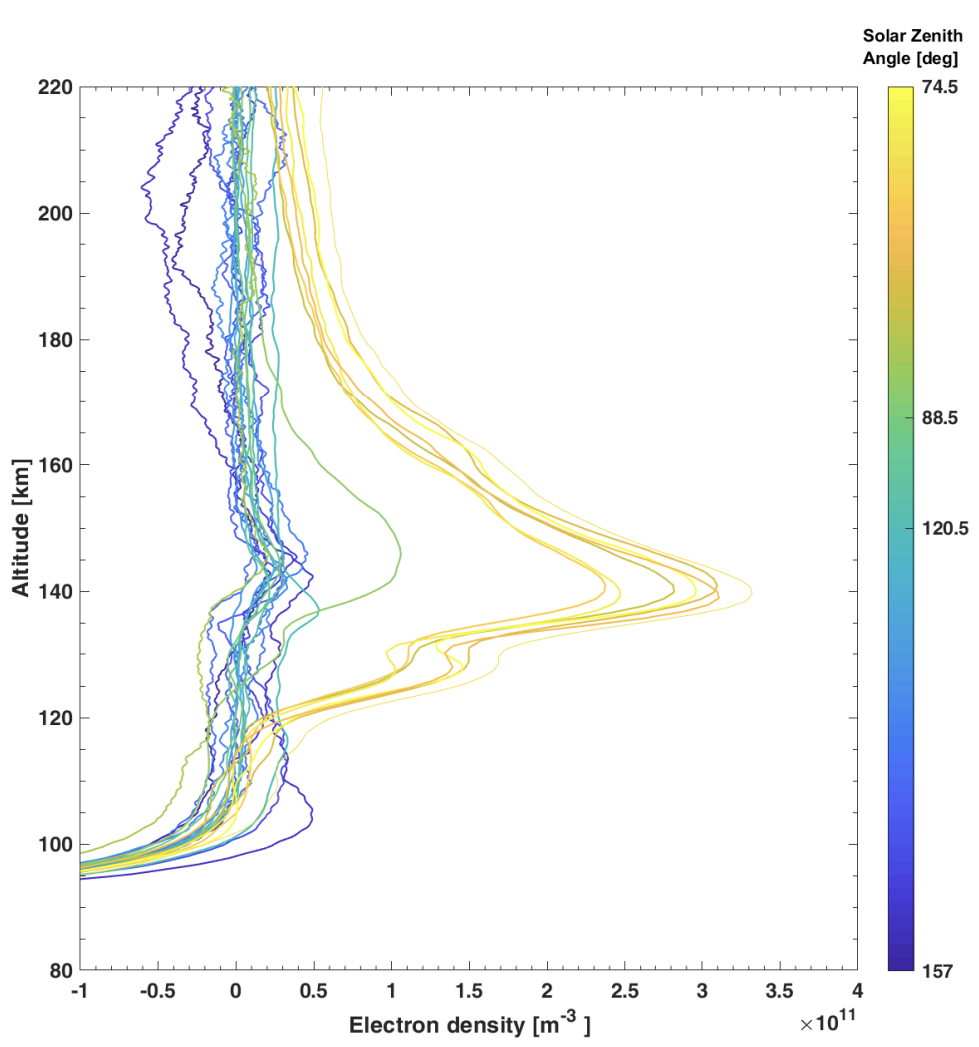
\includegraphics[width=\linewidth]{fig/electron density solar.png}
%         \caption{Electron density measured for different solar zenith angles}
%         \label{fig:electron-density-2}
%     \end{subfigure}

    \caption{Electron density vs. altitude: (a) at different time instances and (b) for different solar zenith angles \cite{gramigna2023venus}.}
    \label{fig:electron-density}
\end{figure}

The total electron content along the path is
\begin{equation}
\mathrm{TEC} = \int_{\text{path}} N_e(s)\, ds
\label{eq:TEC}
\end{equation}
where \(N_e(s)\) is the electron density along the signal path. A numerical tool was used to evaluate atmospheric and ionospheric losses for different elevation angles and altitudes, including the lowest operational altitude of \(52~\mathrm{km}\). Combining the conservative ionospheric model with atmospheric gas and cloud losses gives a maximum total propagation loss of \(L_{\mathrm{gasses,ionosphere}} = 2.5~\mathrm{dB}\), which is used in the UHF link budget.

\medskip
% \noindent A separate rain attenuation term is not included in the link budget. Although sulfuric-acid droplets may fall through the Venusian cloud layer, their effect is already covered by the atmospheric/cloud attenuation term for $\mathrm{H_2SO_4}$ aerosols and droplets. At UHF, the signal wavelength is much larger than the expected droplet size, so additional attenuation due specifically to precipitation is assumed to be small and is included within the atmospheric-loss uncertainty and link margin.
% add this text for clarity later
%Faraday rotation, group delay, phase advance(= average/total phase shift due to TEC, while Phase scintillation = rapid variation of that phase shift due to changing TEC), and Doppler-like ionospheric effects must be analyzed under polarization, synchronization, and receiver tracking requirement
%reflection and diffraction effect can be ignored for line of sight com
%scattering included in db/km of cloud/atmospheric attenuation
\medskip
\noindent Scintillation is not treated as a fixed atmospheric attenuation, but as a fade margin. 
% Since the aerobot-orbiter link operates at UHF, ionospheric scintillation may cause  short-term amplitude and phase fluctuations, especially at low elevation angles where the slant path through the atmosphere and ionosphere is longest. 
Therefore a 2 dB fading margin is incorporated in accordance with SMAD\cite{wertz1999smad}.
%note: Scintillation is not an average attenuation loss.
%It is a temporary fluctuation in received power and phase.
The total atmospheric attenuation due to the earth is given to be $0.3dB$ for operational conditions, and $0.5 dB$ in case of moderate rain\cite{brizzolari2024dsa4attenuation}. 
\subsection{antenna options}

The aerobot operates at UHF and has limited attitude control, so the antenna must provide broad, non-directional coverage rather than high directivity. Wire antennas are therefore the most suitable class because they are simple, lightweight, mechanically robust, and easier to integrate on a balloon gondola. Printed antennas are possible but become relatively large at UHF, while array and aperture antennas are rejected because they add complexity, pointing requirements, mass, and power demand. A two-antenna configuration is selected, with antennas placed near opposite top edges of the gondola to improve low-elevation visibility, reduce blockage during gondola tilt, and relax attitude-control requirements.

The antenna trade-off in \autoref{tab:antenna_tradeoff} assumes that local reflectors or large backplanes are avoided. Although these could reduce radiation toward Venus, they would also make the antenna pattern more directional and could degrade the low-elevation coverage needed during orbiter passes.

% \begingroup
% \scriptsize
% \renewcommand{\arraystretch}{1.18}
% \setlength{\tabcolsep}{2pt}

% \begin{longtable}{|p{0.045\textwidth}|p{0.115\textwidth}|p{0.17\textwidth}|p{0.13\textwidth}|p{0.13\textwidth}|p{0.12\textwidth}|p{0.105\textwidth}|p{0.11\textwidth}|p{0.1\textwidth}|}
% \caption{Scored feasible antenna type trade-off for the aerobot.}
% \label{tab:antenna_tradeoff} \\
% \hline
% \textbf{ID} &
% \textbf{Option$\downarrow$ / Criteria$\rightarrow$} &
% \textbf{Coverage / Visibility (30\%)} &
% \textbf{Gain Performance (5\%)} &
% \textbf{Pointing Loss Performance (25\%)} &
% \textbf{Polarization Loss Performance (15\%)} &
% \textbf{Mass / Integration (10\%)} &
% \textbf{Reliability (15\%)} &
% \textbf{Weighted score} \\
% \hline
% \endfirsthead

% \hline
% \textbf{ID} &
% \textbf{Option$\downarrow$ / Criteria$\rightarrow$} &
% \textbf{Coverage / Visibility (30\%)} &
% \textbf{Gain Performance (5\%)} &
% \textbf{Pointing Loss Performance (25\%)} &
% \textbf{Polarization Loss Performance (15\%)} &
% \textbf{Mass / Integration (10\%)} &
% \textbf{Reliability (15\%)} &
% \textbf{Weighted score} \\
% \hline
% \endhead

% \hline
% \multicolumn{9}{r}{\small Continued on next page} \\
% \endfoot

% \hline
% \endlastfoot

% ANT-1 &
% \textbf{Helical-ring / Huygens-source antenna\cite{morlaas2015helical}} &
% \cellcolor{score5!40}\textbf{5} -- Provides hemispherical coverage without requiring a large reflector as seen in \autoref{fig:helical-ring}, reducing radiation toward the Venus surface while maintaining broad useful coverage toward the orbiter. &
% \cellcolor{score4!40}\textbf{4} -- Moderate useful gain; the ideal Huygens-source pattern has a maximum directivity of about $4.77\,\mathrm{dBi}$, while still preserving broad angular coverage. &
% \cellcolor{score5!40}\textbf{5} -- Low pointing losses over the desired half-space due to the broad cardioid-like radiation pattern, making it attractive for a tilting or swinging gondola. &
% \cellcolor{score5!40}\textbf{5} -- Provides circular polarization over a wide angular region, reducing sensitivity to gondola rotation and polarization mismatch. &
% \cellcolor{score4!40}\textbf{4} -- Compact compared with reflector-backed solutions, but more complex to design, tune, feed, and manufacture than simple dipole-based antennas. &
% \cellcolor{score3!40}\textbf{3} -- Promising performance, but much lower heritage than crossed dipoles, monopoles, or quadrifilar helices. &
% \cellcolor{score5!40}\textbf{4.55} \\
% \hline

% ANT-2 &
% \textbf{Crossed drooping dipole} &
% \cellcolor{score4!40}\textbf{4} -- Provides improved low-elevation coverage compared with a standard crossed dipole, making it well suited for communication near the start and end of an orbiter pass. &
% \cellcolor{score3!40}\textbf{3} -- Still a low-gain antenna, but the drooped geometry directs more useful radiation toward lower elevation angles. &
% \cellcolor{score5!40}\textbf{5} -- Very good option for reducing pointing losses at low elevation angles, which are critical for maximizing the useful orbiter visibility window. &
% \cellcolor{score4!40}\textbf{4} -- Can provide circular polarization, reducing sensitivity to gondola rotation and polarization mismatch with the orbiter. &
% \cellcolor{score3!40}\textbf{3} -- More difficult to integrate than a standard crossed dipole because the drooped elements require additional clearance and mechanical support near the gondola edges. &
% \cellcolor{score5!40}\textbf{5} -- High reliability for non-pointed communication, especially when two antennas are placed on opposite top edges to reduce blockage and tilt sensitivity. &
% \cellcolor{score4!40}\textbf{4.25} \\
% \hline

% ANT-3 &
% \textbf{Quadrifilar helix} &
% \cellcolor{score4!40}\textbf{4} -- Provides broad upper-hemisphere coverage and circular polarization, making it suitable for communication with an orbiter over a wide range of gondola orientations. &
% \cellcolor{score3!40}\textbf{3} -- Low-to-moderate gain; generally better suited for wide coverage than high-gain communication. &
% \cellcolor{score4!40}\textbf{4} -- Pointing losses are low due to the broad radiation pattern, although low-elevation performance depends on the exact helix geometry. &
% \cellcolor{score5!40}\textbf{5} -- Naturally suited for circular polarization, reducing polarization mismatch during gondola rotation or swing. &
% \cellcolor{score2!40}\textbf{2} -- More bulky and mechanically complex than dipole-based options, especially at UHF frequencies. &
% \cellcolor{score4!40}\textbf{4} -- Good heritage for satellite-style communication, but the larger three-dimensional structure may be harder to protect and integrate on the gondola edge. &
% \cellcolor{score4!40}\textbf{3.90} \\
% \hline

% ANT-4 &
% \textbf{Crossed dipole / turnstile} &
% \cellcolor{score4!40}\textbf{4} -- Provides broad angular coverage, as seen in \autoref{fig:crossed-dipole}. With edge mounting, the gondola side may behave more like the reflector-influenced case, while the open side remains closer to the free-space case. &
% \cellcolor{score2!40}\textbf{2} -- Low-gain antenna; suitable for wide coverage, but the orbiter must provide sufficient receive sensitivity or antenna gain to close the link. &
% \cellcolor{score4!40}\textbf{4} -- Pointing losses are generally low due to the broad radiation pattern, but can increase near the horizon or in weak-pattern directions. &
% \cellcolor{score4!40}\textbf{4} -- Circular polarization reduces sensitivity to gondola rotation and can give near-zero polarization loss if the orbiter antenna has matching handedness. &
% \cellcolor{score5!40}\textbf{5} -- Low mass and simple integration; the radiating elements can be very lightweight at UHF frequencies. Each dipole is approximately $0.5\lambda$ long. &
% \cellcolor{score5!40}\textbf{5} -- Reliable, simple, and heritage-friendly, but it radiates more power into the undesired half-space than hemispherical antenna concepts. &
% \cellcolor{score4!40}\textbf{4.15} \\
% \hline

% ANT-5 &
% \textbf{Circularly polarized patch / crossed-slot patch} &
% \cellcolor{score2!40}\textbf{2} -- Provides good broadside upper-hemisphere coverage, but low-elevation coverage is poorer than for wire antennas unless the antenna is carefully shaped or tilted. &
% \cellcolor{score4!40}\textbf{4} -- Can provide higher useful gain than an unbacked wire antenna in its main beam, but this comes at the cost of reduced angular coverage. &
% \cellcolor{score2!40}\textbf{2} -- Pointing losses can become significant when the gondola tilts or when the orbiter is near the edge of the patch beam. &
% \cellcolor{score4!40}\textbf{4} -- Can be designed for circular polarization, giving low polarization loss if the orbiter antenna has matching handedness. &
% \cellcolor{score2!40}\textbf{2} -- Low-profile and easy to protect from the environment, but at UHF it requires a relatively large surface or ground plane, making edge integration less attractive. &
% \cellcolor{score3!40}\textbf{3} -- Mechanically robust and easy to seal, but less reliable for non-pointed communication because its radiation pattern is more directional. &
% \cellcolor{score3!40}\textbf{2.55} \\
% \hline

% ANT-6 &
% \textbf{Quarter-wave monopole} &
% \cellcolor{score3!40}\textbf{3} -- Provides omnidirectional azimuth coverage, but its pattern depends strongly on the ground plane. Edge mounting creates an asymmetric ground plane, which can distort the radiation pattern. &
% \cellcolor{score2!40}\textbf{2} -- Low-gain antenna with limited link margin. It can radiate efficiently with a good ground plane, but this is harder to guarantee at the gondola edge. &
% \cellcolor{score3!40}\textbf{3} -- Pointing losses are low for azimuthal rotation, but can increase when the gondola tilts or when the orbiter lies near the monopole null. &
% \cellcolor{score1!40}\textbf{1} -- Usually linearly polarized, making it more sensitive to orientation and causing additional polarization loss if the orbiter uses circular polarization. &
% \cellcolor{score5!40}\textbf{5} -- Very simple and lightweight; the radiator length is approximately $0.25\lambda$, but a suitable ground plane or counterpoise is required. &
% \cellcolor{score4!40}\textbf{4} -- Mechanically simple and heritage-proven, but less robust to attitude changes, polarization mismatch, and asymmetric edge mounting than circularly polarized options. &
% \cellcolor{score3!40}\textbf{3.00} \\
% \hline

% \end{longtable}
% \endgroup
\begingroup
\scriptsize
\renewcommand{\arraystretch}{1.15}
\setlength{\tabcolsep}{2pt}

\begin{longtable}{|p{0.045\textwidth}|p{0.115\textwidth}|p{0.17\textwidth}|p{0.13\textwidth}|p{0.13\textwidth}|p{0.12\textwidth}|p{0.105\textwidth}|p{0.11\textwidth}|p{0.1\textwidth}|}
\caption{Scored feasible antenna type trade-off for the aerobot.}
\label{tab:antenna_tradeoff} \\
\hline
\textbf{ID} &
\textbf{Option$\downarrow$ / Criteria$\rightarrow$} &
\textbf{Coverage / Visibility (30\%)} &
\textbf{Gain Performance (5\%)} &
\textbf{Pointing Loss Performance (25\%)} &
\textbf{Polarization Loss Performance (15\%)} &
\textbf{Mass / Integration (10\%)} &
\textbf{Reliability (15\%)} &
\textbf{Weighted score} \\
\hline
\endfirsthead

\hline
\textbf{ID} &
\textbf{Option$\downarrow$ / Criteria$\rightarrow$} &
\textbf{Coverage / Visibility (30\%)} &
\textbf{Gain Performance (5\%)} &
\textbf{Pointing Loss Performance (25\%)} &
\textbf{Polarization Loss Performance (15\%)} &
\textbf{Mass / Integration (10\%)} &
\textbf{Reliability (15\%)} &
\textbf{Weighted score} \\
\hline
\endhead

\hline
\multicolumn{9}{r}{\small Continued on next page} \\
\endfoot

\hline
\endlastfoot

ANT-1 &
\textbf{Helical-ring / Huygens-source antenna\cite{morlaas2015helical}} &
\cellcolor{score5!40}\textbf{5} -- Hemispherical coverage; limits radiation toward Venus while maintaining broad orbiter visibility. &
\cellcolor{score4!40}\textbf{4} -- Moderate useful gain; ideal Huygens-source directivity is about $4.77\,\mathrm{dBi}$. &
\cellcolor{score5!40}\textbf{5} -- Broad cardioid-like pattern gives low loss for gondola tilt or swing. &
\cellcolor{score5!40}\textbf{5} -- Circular polarization over a wide angular region reduces rotation mismatch. &
\cellcolor{score4!40}\textbf{4} -- Compact, but harder to tune, feed, and manufacture than simple wire antennas. &
\cellcolor{score3!40}\textbf{3} -- Promising, but lower heritage than dipoles, monopoles, or quadrifilar helices. &
\cellcolor{score5!40}\textbf{4.55} \\
\hline

ANT-2 &
\textbf{Crossed drooping dipole} &
\cellcolor{score4!40}\textbf{4} -- Good low-elevation coverage, useful near start and end of orbiter passes. &
\cellcolor{score3!40}\textbf{3} -- Low gain, but drooping improves radiation toward low elevations. &
\cellcolor{score5!40}\textbf{5} -- Very good low-elevation pointing robustness during visibility windows. &
\cellcolor{score4!40}\textbf{4} -- Can provide circular polarization and reduce gondola-rotation mismatch. &
\cellcolor{score3!40}\textbf{3} -- Needs clearance and support for drooped elements near gondola edges. &
\cellcolor{score5!40}\textbf{5} -- Reliable non-pointed option, especially with two edge-mounted antennas. &
\cellcolor{score4!40}\textbf{4.25} \\
\hline

ANT-3 &
\textbf{Quadrifilar helix} &
\cellcolor{score4!40}\textbf{4} -- Broad upper-hemisphere coverage with good orientation tolerance. &
\cellcolor{score3!40}\textbf{3} -- Low-to-moderate gain; optimized more for coverage than directivity. &
\cellcolor{score4!40}\textbf{4} -- Broad beam gives low pointing loss, but low-elevation performance depends on geometry. &
\cellcolor{score5!40}\textbf{5} -- Naturally circularly polarized, reducing rotation and swing mismatch. &
\cellcolor{score2!40}\textbf{2} -- Bulky and mechanically complex at UHF compared with dipole concepts. &
\cellcolor{score4!40}\textbf{4} -- Good satellite heritage, but harder to protect and integrate on gondola edge. &
\cellcolor{score4!40}\textbf{3.90} \\
\hline

ANT-4 &
\textbf{Crossed dipole / turnstile} &
\cellcolor{score4!40}\textbf{4} -- Broad angular coverage; edge mounting may distort the pattern. &
\cellcolor{score2!40}\textbf{2} -- Low gain; requires sufficient orbiter receiver sensitivity or gain. &
\cellcolor{score4!40}\textbf{4} -- Generally low pointing loss, but weak directions can occur near the horizon. &
\cellcolor{score4!40}\textbf{4} -- Circular polarization possible with matching handedness at the orbiter. &
\cellcolor{score5!40}\textbf{5} -- Very lightweight and simple; each dipole is about $0.5\lambda$. &
\cellcolor{score5!40}\textbf{5} -- Simple and heritage-friendly, but wastes power into undesired half-space. &
\cellcolor{score4!40}\textbf{4.15} \\
\hline

ANT-5 &
\textbf{Circularly polarized patch / crossed-slot patch} &
\cellcolor{score2!40}\textbf{2} -- Good broadside coverage, but weaker low-elevation visibility. &
\cellcolor{score4!40}\textbf{4} -- Higher main-beam gain, but at the cost of angular coverage. &
\cellcolor{score2!40}\textbf{2} -- Sensitive to gondola tilt and orbiter position near beam edge. &
\cellcolor{score4!40}\textbf{4} -- Circular polarization possible with matching orbiter handedness. &
\cellcolor{score2!40}\textbf{2} -- Low profile, but UHF size and ground-plane needs complicate edge mounting. &
\cellcolor{score3!40}\textbf{3} -- Mechanically robust, but less reliable for non-pointed communication. &
\cellcolor{score3!40}\textbf{2.55} \\
\hline

ANT-6 &
\textbf{Quarter-wave monopole} &
\cellcolor{score3!40}\textbf{3} -- Omnidirectional in azimuth, but ground-plane distortion is likely. &
\cellcolor{score2!40}\textbf{2} -- Low gain and limited link margin without a good ground plane. &
\cellcolor{score3!40}\textbf{3} -- Robust to azimuth rotation, but tilt and pattern nulls can increase loss. &
\cellcolor{score1!40}\textbf{1} -- Usually linearly polarized, causing mismatch with circularly polarized links. &
\cellcolor{score5!40}\textbf{5} -- Very simple and light; radiator length is about $0.25\lambda$. &
\cellcolor{score4!40}\textbf{4} -- Heritage-proven, but weak against attitude changes and polarization mismatch. &
\cellcolor{score3!40}\textbf{3.00} \\
\hline

\end{longtable}
\endgroup
\begin{figure}[H]
    \centering
    \begin{subfigure}[t]{0.31\linewidth}
        \centering
        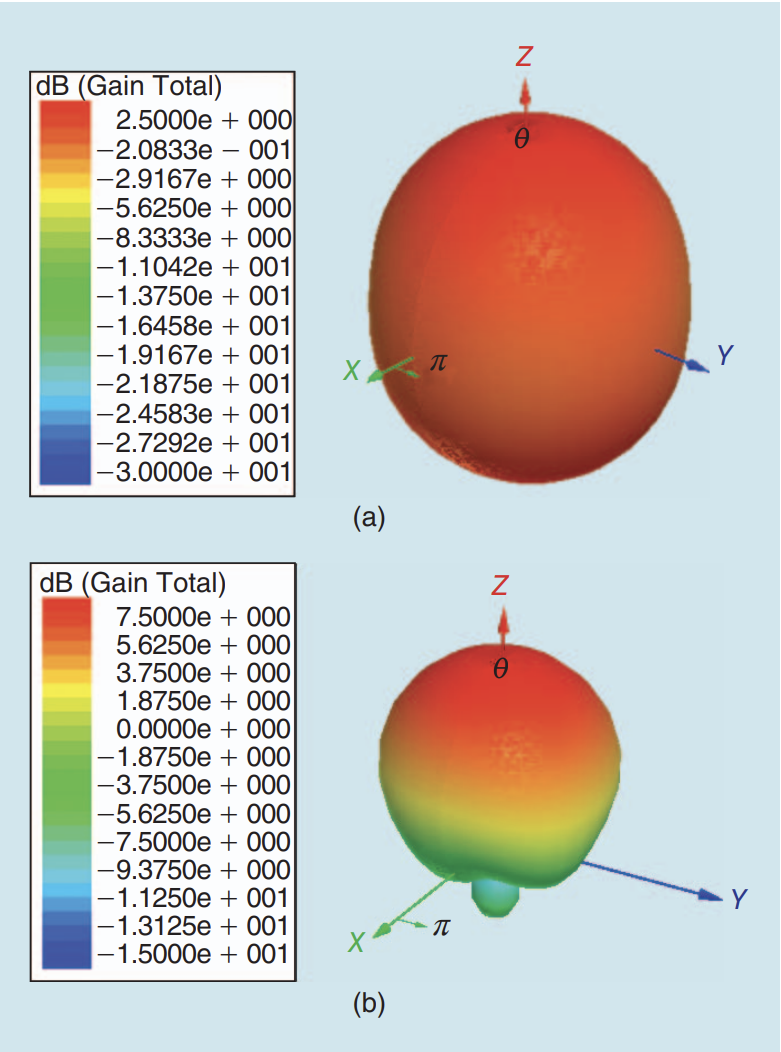
\includegraphics[width=\linewidth]{fig/crossed-dipole.png}
        \caption{Turnstile antenna radiation patterns in free space and above a finite PEC surface~\cite{ta2015crossedDipole}.}
        \label{fig:crossed-dipole}
    \end{subfigure}
    \hfill
    \begin{subfigure}[t]{0.31\linewidth}
        \centering
        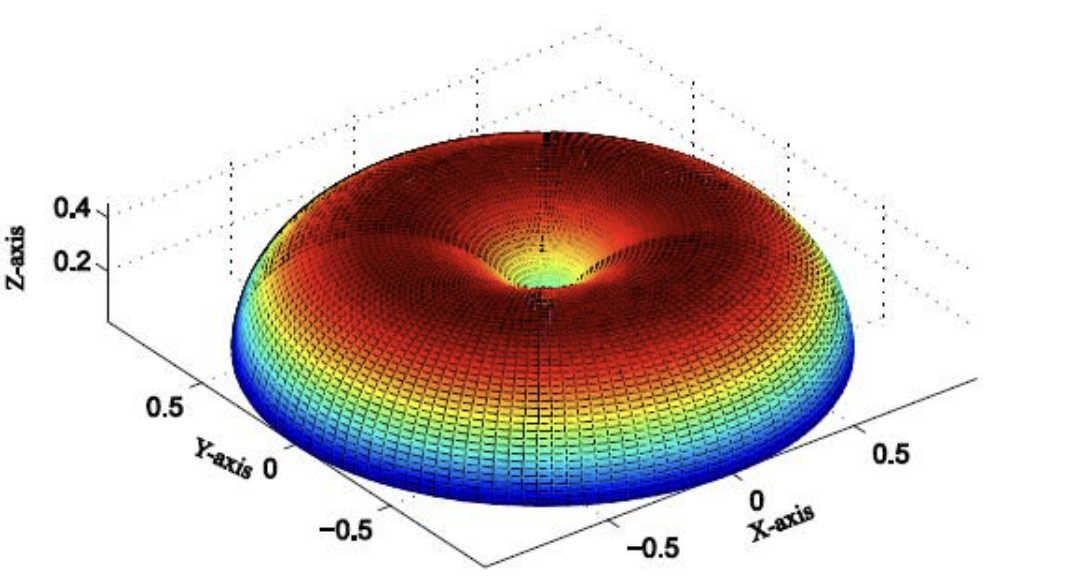
\includegraphics[width=\linewidth]{fig/Quarter wave monopole.png}
        \caption{Radiation pattern of a quarter-wave monopole above virtual ground~\cite{khan2014radiation}.}
        \label{fig:quarter-wave-monopole}
    \end{subfigure}
    \hfill
    \begin{subfigure}[t]{0.31\linewidth}
        \centering
        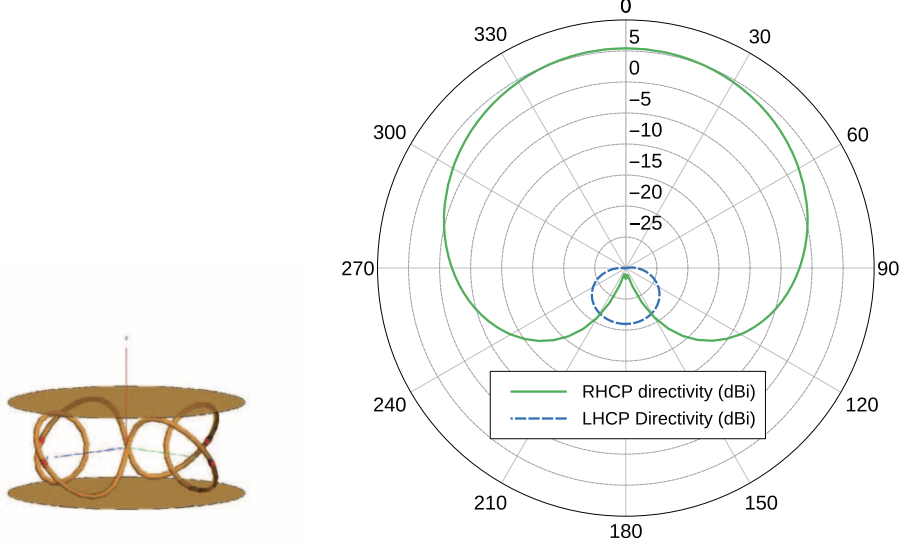
\includegraphics[width=\linewidth]{fig/ring helical.png}
        \caption{Helical-ring antenna geometry and directivity pattern~\cite{morlaas2015helical}.}
        \label{fig:helical-ring}
    \end{subfigure}
    \caption{Representative antenna concepts considered for the aerobot UHF relay link.}
    \label{fig:aerobot_antenna_concepts}
\end{figure}

Based on \autoref{tab:antenna_tradeoff}, the helical-ring/Huygens-source antenna is selected as the baseline because it provides broad hemispherical coverage, circular polarization, moderate useful gain, and low pointing sensitivity. Its main drawback is lower heritage compared with simpler dipole or monopole concepts, so additional prototyping and antenna-pattern verification are required in later design phases.
Based on \autoref{tab:antenna_tradeoff}, the helical-ring was chosen due to its performance despite having slightly lower reliability due to low heritage. 
The trade off table for the best options for the orbiter UHF antenna is shown in \autoref{tab:orbiter_UHF_antenna_tradeoff}.

\begin{table}[H]
\centering
\normalsize
\caption{Scored feasible UHF antenna type trade-off for the orbiter.}
\label{tab:orbiter_UHF_antenna_tradeoff}
\renewcommand{\arraystretch}{1.25}
\setlength{\tabcolsep}{2pt}
\resizebox{\textwidth}{!}{%
\begin{tabular}{|p{1.2cm}|p{3.0cm}|p{4.0cm}|p{3.5cm}|p{3.8cm}|p{3.7cm}|p{3.5cm}|p{3.8cm}|p{2.0cm}|}
\hline
\textbf{ID} &
\textbf{Option$\downarrow$ / Criteria$\rightarrow$} &
\textbf{Nadir Coverage / Visibility (30\%)} &
\textbf{Gain / Link Margin (20\%)} &
\textbf{Pointing Sensitivity (15\%)} &
\textbf{Polarization Performance (15\%)} &
\textbf{Mass / Integration (10\%)} &
\textbf{Reliability / Heritage (10\%)} &
\textbf{Weighted score} \\
\hline

ORB-1 &
\textbf{Quadrifilar helix} &
\cellcolor{score5!40}\textbf{5} -- Provides broad nadir-facing coverage, making it well suited for communication with an aerobot over a large part of the orbiter pass. &
\cellcolor{score4!40}\textbf{4} -- Provides low-to-moderate gain with good useful coverage; suitable for relay links where the orbiter antenna does not need to be highly directional. &
\cellcolor{score5!40}\textbf{5} -- Low pointing sensitivity due to its broad beam, while still benefiting from the orbiter's attitude control. &
\cellcolor{score5!40}\textbf{5} -- Naturally provides circular polarization, reducing polarization mismatch with a rotating or swinging aerobot antenna. &
\cellcolor{score3!40}\textbf{3} -- More bulky than a patch or simple dipole, but still practical for an orbiter-mounted UHF relay antenna. &
\cellcolor{score5!40}\textbf{5} -- Strong heritage for planetary relay communication, making it the most conservative baseline option. &
\cellcolor{score5!40}\textbf{4.60} \\
\hline

ORB-2 &
\textbf{Circularly polarized patch / patch array} &
\cellcolor{score3!40}\textbf{3} -- Provides good nadir-facing coverage, but the beam is generally more directional than a quadrifilar helix. Coverage near the edge of the pass may be weaker. &
\cellcolor{score5!40}\textbf{5} -- Can provide higher gain than a single low-gain wire antenna, especially if multiple patch elements are used. &
\cellcolor{score3!40}\textbf{3} -- Moderate pointing sensitivity; acceptable for an orbiter with attitude control, but less forgiving than a broad helical antenna. &
\cellcolor{score4!40}\textbf{4} -- Can be designed for circular polarization, giving good polarization compatibility with the aerobot link. &
\cellcolor{score5!40}\textbf{5} -- Low-profile and easy to mount on a spacecraft panel, but may require a larger surface area or array for sufficient coverage and gain. &
\cellcolor{score4!40}\textbf{4} -- Good antenna heritage in space applications, but relay coverage must be verified carefully for the required pass geometry. &
\cellcolor{score4!40}\textbf{3.85} \\
\hline

ORB-3 &
\textbf{Crossed dipole / turnstile array} &
\cellcolor{score4!40}\textbf{4} -- Can provide broad coverage if arranged properly, but the pattern depends strongly on the spacecraft mounting geometry and array configuration. &
\cellcolor{score3!40}\textbf{3} -- Low-to-moderate gain; multiple elements may be required to improve link margin or shape the nadir coverage. &
\cellcolor{score4!40}\textbf{4} -- Low pointing sensitivity if designed as a broad-beam array, but less controlled than a dedicated nadir-facing helix or patch system. &
\cellcolor{score4!40}\textbf{4} -- Can provide circular polarization if the crossed elements are fed with the correct phase relationship. &
\cellcolor{score3!40}\textbf{3} -- Lightweight elements, but array phasing, cabling, and deployment or mounting may increase integration complexity. &
\cellcolor{score3!40}\textbf{3} -- Reasonable heritage, but less straightforward as an orbiter relay antenna than a quadrifilar helix or patch design. &
\cellcolor{score4!40}\textbf{3.60} \\
\hline

ORB-4 &
\textbf{Helical-ring / Huygens-source antenna} &
\cellcolor{score4!40}\textbf{4} -- Provides broad hemispherical coverage while reducing radiation away from the desired half-space, making it conceptually attractive for nadir-facing relay communication. &
\cellcolor{score4!40}\textbf{4} -- Moderate useful gain with broad coverage; attractive if the design can be tuned to the required UHF band and spacecraft mounting geometry. &
\cellcolor{score4!40}\textbf{4} -- Low pointing sensitivity over the desired hemisphere due to its broad cardioid-like pattern. &
\cellcolor{score5!40}\textbf{5} -- Provides circular polarization over a wide angular region, which is favourable for communication with a moving or rotating aerobot. &
\cellcolor{score3!40}\textbf{3} -- Compact compared with reflector-backed solutions, but more complex to tune, feed, and qualify than conventional options. &
\cellcolor{score2!40}\textbf{2} -- Promising but lower heritage; would require mission-specific prototyping and qualification before being selected as the orbiter baseline. &
\cellcolor{score4!40}\textbf{3.85} \\
\hline

ORB-5 &
\textbf{Simple monopole / dipole} &
\cellcolor{score3!40}\textbf{3} -- Provides broad coverage, but the pattern may be strongly affected by the spacecraft body and may not be well shaped toward nadir. &
\cellcolor{score2!40}\textbf{2} -- Low gain and limited link margin; more suitable as a backup or contingency antenna than as the main relay antenna. &
\cellcolor{score3!40}\textbf{3} -- Low pointing sensitivity in some directions, but pattern nulls and spacecraft blockage can reduce performance. &
\cellcolor{score1!40}\textbf{1} -- Usually linearly polarized, causing additional loss if the aerobot antenna uses circular polarization. &
\cellcolor{score5!40}\textbf{5} -- Very simple, lightweight, and easy to integrate, especially as a backup antenna. &
\cellcolor{score4!40}\textbf{4} -- Mechanically reliable and simple, but less suitable as the primary relay antenna due to lower gain, polarization mismatch, and less controlled coverage. &
\cellcolor{score3!40}\textbf{2.80} \\
\hline

\end{tabular}%
}
\end{table}
From this trade-off, the orbiter UHF antenna had the quadrifilar helix antenna as a clear best option. For communication between earth and the Venus orbiter, a high-gain parabolic dish was chosen. This is the standard deep-space option. It provides high directivity and a high link margin for communication with Earth-based ESTRACK stations.
\subsection{link budget iterative process}
\label{subsec: link budget iterative process}
For the link budget, the end-to-end BER is approximated as the sum of the BER contributions of the individual communication links. Therefore, the BER allocation for the aerobot--orbiter link is chosen to be at least as strict as that of the orbiter--Earth link, such that the total system requirement of $\mathrm{BER} \leq 10^{-6}$ is satisfied. The aerobot--orbiter link is the most design-driving part of the communication system, since the aerobot is more constrained in mass, volume, and available transmitter power than the orbiter. The required aerobot data rate is taken as $R_b = 1500~bits/s$.

The aerobot UHF transmit antenna gain, orbiter UHF receive antenna gain, and receiver system noise temperature are taken from the previous subsystem estimates. For each candidate modulation, the number of bits per symbol, $m$, is defined. Together with the FEC code rate, $\rho$, and the roll-off factor, $\alpha$, this determines the spectral efficiency as shown in \autoref{eq:spectral_efficiency} \cite{wertz1999smad}:
\begin{equation}
    \eta = \frac{m\rho}{1+\alpha}
    \label{eq:spectral_efficiency}
\end{equation}
where $\eta$ is the spectral efficiency in $bits/s/Hz$. The required bandwidth can then be estimated from the selected bit rate and spectral efficiency.

For different required BER , the required uncoded value of $E_b/N_0$ is first determined from the modulation performance. A coding gain is then applied based on the selected FEC code rate and coding scheme. The resulting required $E_b/N_0$ is converted to the required carrier-to-noise ratio using \autoref{eq:receiver_signal_to_noise}:
\begin{equation}
    \frac{C}{N} = \frac{E_b}{N_0}\frac{R_b}{B}
    \label{eq:receiver_signal_to_noise}
\end{equation}
where $B$ is the occupied bandwidth. This required $C/N$ is then used in the link budget to determine the required aerobot transmitter power, $P_t$ using the link budget. The maximum distance and propagation losses between the aerobot and orbiter are assumed. 

\section{communication system design}
Based on \autoref{subsec: link budget iterative process}, the required RF power was evaluated for different BER and coding options and compared with available space-grade transceivers. The GAUSS high-power UHF transceiver is selected for the aerobot because it covers the required UHF relay band, supports the selected MSK/GMSK-type modulation and FEC options, and provides sufficient data-rate and RF-power margin for the \(1500~\mathrm{bit/s}\) aerobot--orbiter link.

% \begin{figure}
%     \centering
%     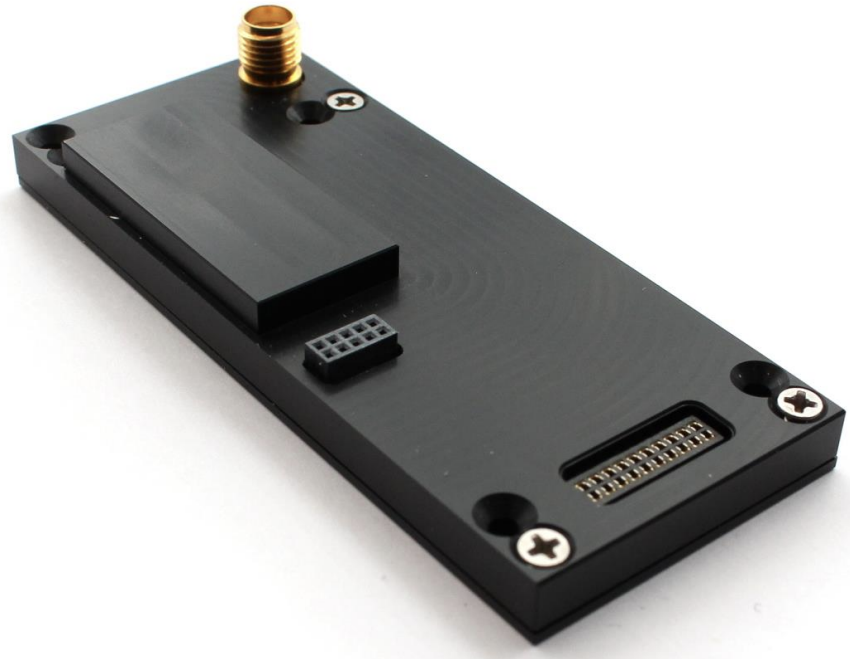
\includegraphics[width=0.2\linewidth]{fig/gauss high power transceiver.png}
%     \caption{Gauss high power transceiver}
%     \label{fig:gauss-transceiver}
% \end{figure}

\begin{table}[H]
\centering
\caption{Main GAUSS high-power UHF radio specifications.}
\label{tab:gauss_uhf_radio_specs}
\scriptsize
\renewcommand{\arraystretch}{1.10}
\setlength{\tabcolsep}{3pt}
\begin{tabular}{|p{3.5cm}|p{9.0cm}|}
\hline
\textbf{Parameter} & \textbf{Value} \\
\hline
Frequency range & RX: 390--500 MHz; TX: 400--450 MHz \\
\hline
RF output power & Software-configurable, 30--40 dBm; maximum specified value of 40.1 dBm at 400 MHz \\
\hline
Data rate & 0.3--250 kbps; current maximum stated as 100 kbps \\
\hline
Sensitivity & \(-122\) dBm at 1.2 kbps; \(-119\) dBm at 9.6 kbps; \(-109\) dBm at 50 kbps \\
\hline
RF efficiency & Typically 40--55\%, up to 59\%, depending on RF output power \\
\hline
Supported modulation / coding & FSK, MSK, GFSK, GMSK; Viterbi, Reed--Solomon FEC, and turbo coding supported \\
\hline
Supply voltage & 3.3 V digital supply and 7--12 V power-amplifier supply \\
\hline
Electrical power usage & Approximately 0.22 W in standby/reception; 17.2--19.6 W at maximum RF output with 12 V PA supply \\
\hline
Mass and size & 37 g; \(75 \times 31.5 \times 12.5~\mathrm{mm}\) \\
\hline
Temperature range & \(-40^\circ\mathrm{C}\) to \(+85^\circ\mathrm{C}\) \\
\hline
\end{tabular}
\end{table}

The orbiter requires a transponder capable of supporting both the UHF proximity relay and the X-band Earth link. The UST-Lite is selected as a representative orbiter transponder because its modular SDR architecture supports deep-space and relay communication, CCSDS-compatible operation, multiple simultaneous channels, and high-rate telemetry interfaces.

\begin{table}[H]
\centering
\caption{Main properties of the UST-Lite transponder.}
\label{tab:ust_lite_transponder_specs}
\scriptsize
\renewcommand{\arraystretch}{1.10}
\setlength{\tabcolsep}{3pt}
\begin{tabular}{|p{3.6cm}|p{8.9cm}|}
\hline
\textbf{Parameter} & \textbf{Value} \\
\hline
Supported links & Direct-to-Earth, user-terminal, and proximity relay communication using modular multi-band SDR architecture \\
\hline
Frequency bands & S, X, K, and Ka bands; UHF module possible for relay applications, assumed approximately 390--450 MHz \\
\hline
Data rates & Up to 100 Mbps; higher data rates available upon request \\
\hline
Modulation & CCSDS-compatible SDR modulation; assumed BPSK/QPSK/OQPSK, GMSK, and higher-order modes depending on configuration \\
\hline
Channel coding & CCSDS and LDPC supported; Reed--Solomon, convolutional, Turbo, and concatenated coding assumed possible from UST heritage \\
\hline
RF output power & Not specified; assumed similar to UST at approximately \(+12~\mathrm{dBm}\), with external power amplifiers required for spacecraft EIRP \\
\hline
Receiver noise figure & Not specified; assumed similar to UST: \(<3.2~\mathrm{dB}\) for S/X/Ka and \(<3.9~\mathrm{dB}\) for UHF \\
\hline
Mass and volume & \(3.4~\mathrm{kg}\) and \(113 \times 121 \times 200~\mathrm{mm}\) for a dual-band configuration; depends on selected bands \\
\hline
Power consumption & 28 V unregulated supply; approximately 35 W typical for a dual-band configuration \\
\hline
Interfaces & 10 Gbps SerDes, \(4\times\) SpaceWire, \(2\times\) JTAG, and \(3\times\) UART \\
\hline
Radiation tolerance & \(40~\mathrm{krad}\) TID; SEL immune up to \(38~\mathrm{MeV\cdot cm^2/mg}\) \\
\hline
Additional capabilities & Up to four full-duplex independent channels, expandable DSP module, clock disciplining, and ranging capability \\
\hline
\end{tabular}
\end{table}
A CCSDS-compatible rate-\(1/2\) turbo code with the 1784-bit information block is selected for all four links. From the CCSDS performance curves, this provides an effective coding gain of approximately \(10~\mathrm{dB}\), as shown in \autoref{fig:coding-gains}, at the cost of increased latency. The proximity aerobot--orbiter links use MSK modulation because its constant-envelope waveform enables efficient nonlinear power amplification and reduces transmitter power consumption. The Earth--orbiter links use BPSK because it is simple, robust at low \(E_b/N_0\), and suitable for low-data-rate deep-space communication. A roll-off factor of \(0.35\) is selected from the link-budget iteration. The final link budgets are shown in \autoref{tab:final_link_budget} and satisfy the minimum link-margin requirements of \(3~\mathrm{dB}\) for downlink and \(6~\mathrm{dB}\) for command links~\cite{chen2006linkSystemDesign}.
%coding schemes + digital modulation types
%total design block diagram
%total link budget

{\scriptsize
\renewcommand{\arraystretch}{1.12}
\setlength{\tabcolsep}{2pt}

\begin{xltabular}{\textwidth}{|
>{\raggedright\arraybackslash}p{3.1cm}|
>{\centering\arraybackslash}p{1.1cm}|
>{\raggedright\arraybackslash}X|
>{\raggedright\arraybackslash}X|
>{\raggedright\arraybackslash}X|
>{\raggedright\arraybackslash}X|}
\caption{Communication subsystem link budget summary.}
\label{tab:final_link_budget}\\

\hline
\textbf{Parameter} &
\textbf{Unit} &
\textbf{Aerobot--Orbiter Uplink} &
\textbf{Orbiter--Aerobot Downlink} &
\textbf{Earth--Orbiter Uplink} &
\textbf{Orbiter--Earth Downlink} \\
\hline
\endfirsthead

\caption[]{Communication subsystem link budget summary continued.}\\
\hline
\textbf{Parameter} &
\textbf{Unit} &
\textbf{Aerobot--Orbiter Uplink} &
\textbf{Orbiter--Aerobot Downlink} &
\textbf{Earth--Orbiter Uplink} &
\textbf{Orbiter--Earth Downlink} \\
\hline
\endhead

\hline
\multicolumn{6}{r}{\textit{Continued on next page}}\\
\endfoot

\hline
\endlastfoot

\multicolumn{6}{|l|}{\textbf{Frequency and transmitter}} \\
\hline
Frequency & MHz / GHz & 391 MHz & 401 MHz & 7.175 GHz & 8.425 GHz \\
\hline
Transmitter type & -- & Aerobot UHF transceiver & UST-Lite UHF module & ESTRACK ground station & UST-Lite X-band module + PA \\
\hline
Transmitter antenna type & -- & Helical-ring antenna & Quadrifilar helix & ESTRACK dish & High-gain parabolic dish \\
\hline
Transmitter antenna gain & dBi & 4.09 & 4.00 & 65.81 & 34.38 \\
\hline
Transmitter RF power, $P_t$ & dBW & 4.71 & 6.99 & 43.01 & 11.30 \\
\hline
Transmitter line loss & dB & 0.50 & 0.50 & 1.00 & 1.00 \\
\hline
Backoff / implementation loss at transmitter & dB & 0.00 & 0.00 & 0.00 & 0.00 \\
\hline
EIRP & dBW & 8.30 & 10.49 & 107.82 & 44.69 \\
\hline

\multicolumn{6}{|l|}{\textbf{Propagation path}} \\
\hline
Propagation range & km & 40 000 & 40 000 & 261 000 000 & 261 000 000 \\
\hline
Free-space path loss & dB & 176.32 & 176.54 & 277.89 & 279.28 \\
\hline
Atmospheric / ionospheric losses & dB & 2.50 & 2.50 & 0.50 & 0.50 \\
\hline
Scintillation / fade margin & dB & 2.00 & 2.00 & 0.00 & 0.00 \\
\hline
Pointing loss & dB & 1.50 & 1.50 & 0.70 & 0.70 \\
\hline
Polarization loss & dB & 0.00 & 0.00 & 0.20 & 0.20 \\
\hline
Combined path loss, $L_{\mathrm{comb}}$ & dB & 182.32 & 182.54 & 279.29 & 280.68 \\
\hline

\multicolumn{6}{|l|}{\textbf{Receiver}} \\
\hline
Receiver type & -- & UST-Lite UHF module & Aerobot UHF transceiver & UST-Lite X-band module & ESTRACK ground station \\
\hline
Receiver antenna type & -- & Quadrifilar helix & Helical-ring antenna & High-gain parabolic dish & ESTRACK dish \\
\hline
Receiver antenna gain & dBi & 4.00 & 4.09 & 32.99 & 67.20 \\
\hline
Receiver line loss & dB & 0.50 & 0.50 & 1.00 & 0.30 \\
\hline
Received carrier power, $C$ & dBW & -170.52 & -168.46 & -139.48 & -169.09 \\
\hline
System noise temperature, $T_s$ & dB-K & 21.76 & 24.77 & 21.76 & 13.98 \\
\hline
Receiver $G/T$ & dB/K & -18.26 & -21.18 & 10.23 & 52.92 \\
\hline
Receiver $C/N_0$ & dB-Hz & 36.32 & 35.36 & 67.36 & 45.53 \\
\hline

\multicolumn{6}{|l|}{\textbf{Data and link performance}} \\
\hline
Data rate, $R_b$ & bit/s & 1500 & 500 & 1500 & 10000 \\
\hline
Data rate, $10\log_{10}(R_b)$ & dB-Hz & 31.76 & 26.99 & 31.76 & 40.00 \\
\hline
Modulation & -- & MSK & MSK & BPSK & BPSK \\
\hline
Code type & -- & Turbo & Turbo & Turbo & Turbo \\
\hline
Code rate, $\rho$ & -- & 0.50 & 0.50 & 0.50 & 0.50 \\
\hline
Roll-off factor, $\alpha$ & -- & 0.35 & 0.35 & 0.35 & 0.35 \\
\hline
Occupied bandwidth & Hz / kHz & 4050 Hz & 1350 Hz & 4050 Hz & 27000 Hz \\
\hline
Available $E_b/N_0$ & dB & 4.56 & 8.37 & 35.60 & 5.53 \\
\hline
Required $E_b/N_0$ & dB & 1.55 & 1.55 & 2.52 & 2.52 \\
\hline
Coding gain & dB & 10.00 & 10.00 & 10.00 & 10.00 \\
\hline
Modem implementation loss & dB & 1.00 & 1.00 & 1.00 & 1.00 \\
\hline
Link margin & dB & 3.01 & 6.83 & 33.08 & 3.01 \\

\end{xltabular}
}
\autoref{tab:final_link_budget} assumes the largest expected communication distances. Although the selected UHF radios can provide up to approximately \(5~\mathrm{W}\) RF output power, the nominal link budget requires only about \(1{-}3~\mathrm{W}\). This power headroom allows operation below the maximum rating, improving thermal reliability and leaving margin for unmodelled effects such as ageing, radiation degradation, temperature-dependent amplifier performance, antenna misalignment, additional line losses, and unexpected propagation losses.




% For the two-plate helical-ring antenna, a pre-margin mass estimate of 60 g is selected. The estimate is based on the compact eight-turn HRA from Morlaas et al.~\cite{morlaas2015}, which has an outer radius of 11.14 mm, an inner radius of 5.57 mm, and a height of 5.57 mm at 1.579 GHz. Scaling this geometry to 400 MHz gives $S_f = 1.579 / 0.400 = 3.9475$, so the scaled outer radius is $R_{out} = 11.14 \cdot 3.9475 = 43.98$ mm and the scaled height is $h = 5.57 \cdot 3.9475 = 21.99$ mm. The helical conductor length is estimated as 0.592 m. For a 2.0 mm diameter copper conductor, the ring mass is $m_{ring} = 8.96 \cdot \pi \cdot (0.10)^2 \cdot 59.2 = 16.7$ g, where the density of copper is 8.96 g/cm$^3$, the wire radius is 0.10 cm, and the length is 59.2 cm. The two loading plates are taken as 0.5 mm thick aluminium disks with radius 4.398 cm, giving $m_{plates} = 2 \cdot 2.70 \cdot \pi \cdot (4.398)^2 \cdot 0.05 = 16.4$ g. An 80 mm by 80 mm by 1.0 mm RF support/feed board with two 35 micrometer copper cladding layers is estimated as $m_{board} = 8 \cdot 8 \cdot 0.10 \cdot 1.85 + 2 \cdot 8 \cdot 8 \cdot 0.0035 \cdot 8.96 = 15.9$ g. Finally, adding 7 g for the connector and feed probes and 4 g for small spacers and fasteners gives $m_{total} = 16.7 + 16.4 + 15.9 + 7 + 4 = 60.0$ g. Therefore, 60 g is used as the pre-margin mass estimate for the two-plate HRA at 390--410 MHz.
The UHF communication subsystem mass budget and peak power estimate are summarized in \autoref{tab:uhf_mass_power_budget}. The mass margins are applied according to ECSS design-margin practice~\cite{ecss2010_design_margins}, while the transmit power represents a conservative worst-case value based on the maximum aerobot--orbiter range; nominal operation is expected to require lower RF power.

\begin{table}[H]
\centering
\small
\caption{Aerobot UHF communication subsystem mass and power budget}
\label{tab:uhf_mass_power_budget}
\renewcommand{\arraystretch}{1.12}
\setlength{\tabcolsep}{4pt}
\begin{tabular}{p{4.5cm} p{3.4cm} c c c}
\hline
\textbf{Mass item} & \textbf{Dimensions / description} & \textbf{Mass [g]} & \textbf{Margin [\%]} & \textbf{Mass after margin [g]} \\
\hline
GAUSS High Power UHF Radio & \(75 \times 31.5 \times 12.5~\mathrm{mm}\) & 37.0 & 10 & 40.7 \\
Two two-plate HRA antennas & \(2 \times (\varnothing 88 \times 22~\mathrm{mm})\) & 120.0 & 20 & 144.0 \\
RF cables, connectors, antenna supports, mounting hardware, and harnessing & Routed integration hardware & 80.0 & 20 & 96.0 \\
\hline
\textbf{Total mass} & -- & \textbf{237.0} & -- & \textbf{280.7} \\
\hline
\multicolumn{5}{c}{} \\
\hline
\textbf{Power mode / item} & \textbf{Description} & \multicolumn{3}{c}{\textbf{Power [W]}} \\
\hline
Required RF output power & Worst-case link-budget value & \multicolumn{3}{c}{2.96} \\
Receive mode & Transceiver receiving only & \multicolumn{3}{c}{0.22} \\
Transmit mode & Estimated maximum operational transmit mode & \multicolumn{3}{c}{6.30} \\
Transmit + receive mode & Simultaneous transmit and receive & \multicolumn{3}{c}{6.52} \\
\hline
\end{tabular}
\end{table}
%block diagram of comms system


\section{Command and Data Handling System Design}

The C\&DH design is preliminary and will be refined once the exact payload data-generation timeline and orbiter contact windows are better known. The current design is driven by low processed payload data rates, intermittent communication, autonomous operation, and the need to store data during no-contact periods. The top-level requirements are listed in \autoref{tab:obc_cdh_requirements}.

\begin{table}[H]
\centering
\caption{Top-level C\&DH/OBC data-handling requirements}
\label{tab:obc_cdh_requirements}
\small
\renewcommand{\arraystretch}{1.15}
\begin{tabular}{p{2.2cm} p{10.8cm}}
\hline
\textbf{ID} & \textbf{Requirement} \\
\hline
REQ-CDH-01 & The C\&DH subsystem shall support an aggregate incoming telemetry rate of at least \(4~\mathrm{kbit/s}\) from payload, IMU, barometer, and housekeeping sources. \\
\hline
REQ-CDH-02 & The C\&DH subsystem shall time-tag all accepted telemetry packets with a time resolution of \(1~\mathrm{s}\) or better. \\
\hline
REQ-CDH-03 & The C\&DH subsystem shall provide at least \(32~\mathrm{MB}\) of usable non-volatile storage for science and housekeeping data. \\
\hline
REQ-CDH-04 & The C\&DH subsystem shall forward stored telemetry to the communication subsystem at a useful output rate of at least \(1500~\mathrm{bit/s}\) during nominal orbiter contact. \\
\hline
REQ-CDH-05 & The C\&DH subsystem shall preserve a protected fault-log and critical-housekeeping memory region of at least \(512~\mathrm{kB}\) during nominal operation and after processor reset. \\
\hline
REQ-CDH-06 & The C\&DH subsystem shall transmit each validated telecommand to the correct payload or subsystem interface within \(5~\mathrm{s}\) of command acceptance during nominal operation. \\
\hline
\end{tabular}
\end{table}

The theoretical storage requirement was estimated using the selected payload duty cycles, instrument data rates, a four-day day/night cycle, continuous barometer operation, and a \(20\%\) daytime orbiter contact window. Science instruments are assumed to operate only during daytime, while barometers operate continuously. Assuming the duty cycles are distributed over the daytime period, the maximum accumulated data volume is approximately \(10~\mathrm{MB}\). A practical storage requirement of \(32{-}130~\mathrm{MB}\) is therefore selected to include margin for burst measurements, packet overhead, missed contacts, and retransmissions. 

\begin{figure}[H]
    \centering
    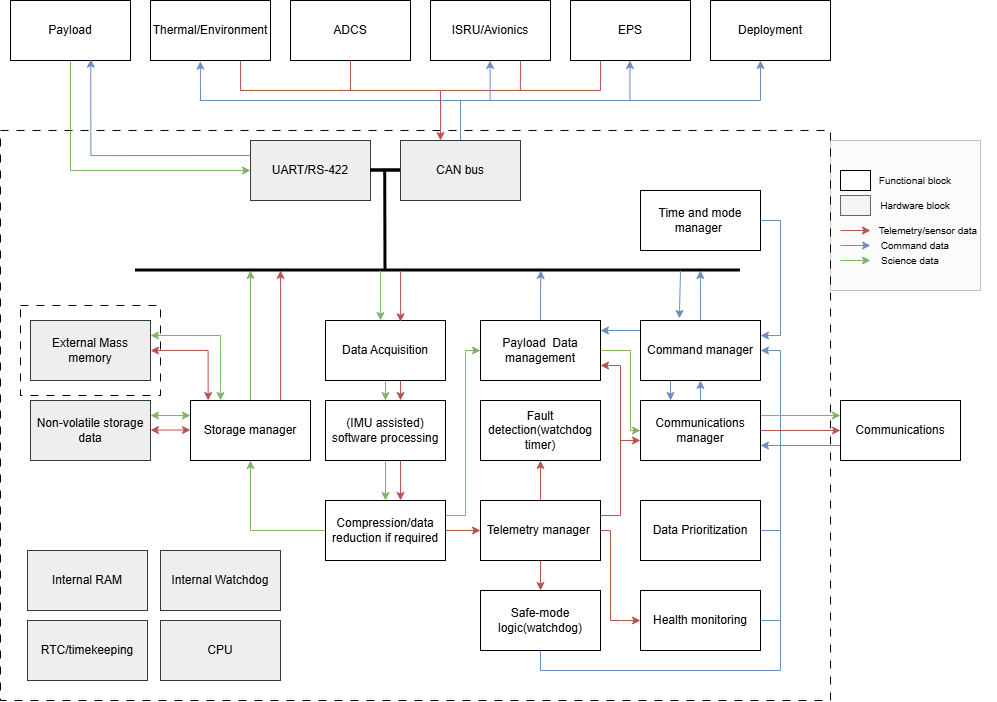
\includegraphics[width=1.0\linewidth]{fig/OBC block diagram.png}
    \caption{Data handling block diagram}
    \label{fig:OBC-block}
\end{figure}

The selected representative OBC is the Alén Space DARA OBC. It agrees with the proposed C\&DH architecture because it integrates the required processor, memory, RTC, watchdog/reset circuit, IMU, board sensors, and subsystem interfaces needed for payload scheduling, telemetry acquisition, IMU-assisted processing, storage management, command handling, health monitoring, and safe-mode recovery. The integrated \(128~\mathrm{MB}\) NAND Flash is selected as the primary science and housekeeping buffer, while the \(512~\mathrm{kB}\) MRAM is reserved for critical status and fault information.

\begin{table}[H]
\centering
\caption{Main properties of the selected DARA OBC}
\label{tab:dara_obc_properties}
\small
\renewcommand{\arraystretch}{1.12}
\begin{tabular}{p{4.0cm} p{8.5cm}}
\hline
\textbf{Property} & \textbf{Value / description} \\
\hline
Processor & ARM Cortex-M7, 32-bit CPU with FPU, up to \(280~\mathrm{MHz}\) \\
\hline
Power and supply & \(280~\mathrm{mW}\) typical, \(3.3~\mathrm{V}\) nominal supply \\
\hline
Program and working memory & \(2~\mathrm{MB}\) program Flash, \(1.4~\mathrm{MB}\) internal RAM, and \(32~\mathrm{MB}\) SDRAM \\
\hline
Persistent storage & \(512~\mathrm{kB}\) MRAM for critical status and \(128~\mathrm{MB}\) NAND Flash for science and housekeeping data \\
\hline
Optional storage & \(2\times\) microSD card slots, up to \(64~\mathrm{GB}\) each \\
\hline
Integrated sensors & IMU with 3-axis magnetometer, gyroscope, and accelerometer; board voltage, current, and temperature sensors \\
\hline
Interfaces & \(3\times\) RS422, \(2\times\) CAN, UART, \(2\times\) I\(^2\)C, SPI, GPIO, ADC, PWM, PPS, and JTAG \\
\hline
Fault recovery and timekeeping & Hardware watchdog/reset circuit and RTC with independent power supply option \\
\hline
Environment, mass, and size & \(-40^\circ\mathrm{C}\) to \(+85^\circ\mathrm{C}\), \(115~\mathrm{g}\), \(93.3 \times 89.3 \times 12.6~\mathrm{mm}\) \\
\hline
\end{tabular}
\end{table}

\section{Sensitivity Analysis}

The design is mainly driven by the aerobot--orbiter communication link budget. Antenna selection affects gain, coverage, pointing loss, and polarization loss, while lower operating frequency reduces free-space path loss but increases antenna size and mass. A stricter BER requirement increases the required \(E_b/N_0\), reducing link margin. Data rate is also critical: since \(E_b/N_0 = C/N_0 - 10\log_{10}(R_b)\), doubling the bit rate reduces the link margin by approximately \(3~\mathrm{dB}\) if all other parameters remain unchanged. The link-budget tool was checked against these expected sensitivities.

The OBC data-handling design is most sensitive to payload data rate, duty cycle, and orbiter contact duration. Higher data generation or shorter contact time increases stored data volume and may prevent the buffer from fully emptying during a pass. However, the selected \(128~\mathrm{MB}\) NAND Flash provides significant margin above the theoretical \(10~\mathrm{MB}\) requirement. The most important parameters to refine later are therefore the real payload operation schedule and orbiter visibility duration.

\section{Verification and Validation}

Verification confirms that the communication and C\&DH designs meet their requirements, while validation confirms suitability for the Venus aerobot mission concept. The communication design tool is verified through sensitivity checks on transmitter power, antenna gain, losses, and data rate, including the relation \(E_b/N_0 = C/N_0 - 10\log_{10}(R_b)\), supporting REQ-COM-04. REQ-COM-01 and REQ-COM-02 are verified through representative transceiver tests under worst-case attenuation, measuring BER and useful data rate. REQ-COM-03 is verified by inspection of frequency band, modulation, coding, and ESTRACK compatibility. REQ-COM-05 is verified through antenna radiation-pattern measurements, orbiter-pass coverage simulation, and environmental testing.

The C\&DH requirements are verified through functional OBC tests. Representative payload, IMU, barometer, and housekeeping data streams verify REQ-CDH-01 and REQ-CDH-02 by checking accepted input rate and time-tagging. REQ-CDH-03 is verified by memory inspection and simulated day/night buffer testing, while REQ-CDH-04 is verified by forwarding stored telemetry to the communication subsystem at \(1500~\mathrm{bit/s}\). REQ-CDH-05 is verified through reset and fault-log tests, and REQ-CDH-06 through command-injection tests that confirm correct routing within the required time.

Validation is performed using mission-level scenarios. The communication subsystem is validated with a representative aerobot--orbiter relay scenario using the selected data rate, modulation, coding, contact duration, and telemetry packets. The OBC is validated through an end-to-end operational scenario including daytime payload duty cycles, continuous barometer operation, no nighttime contact, limited daytime orbiter contact, realistic data streams, and command updates. Successful validation shows that the combined communication and C\&DH design supports autonomous operation, data storage, downlink during contact windows, critical-data preservation, and safe-mode recovery.
\chapter{Thermal and Environmental Control}
\label{ch:thermal_environmental_control}
\section{Subsystem Scope and Design Drivers}
\label{sec:tcs_scope}
The Thermal and Environmental Control subsystem is responsible for maintaining the aerobot components within their allowable temperature ranges while protecting exposed hardware from the harsh Venus environment. This includes thermal control of the gondola, payload, power system, ISRU equipment, sampling hardware, and selected balloon-envelope interfaces.
% In addition to heating and cooling, the subsystem must address chemical resistance, ultraviolet degradation, and long-duration environmental exposure.
The main design drivers are:
\vspace{-5pt}
\begin{itemize}[itemsep=1pt, parsep=1pt]
    \item long-duration operation in the Venus cloud layer
    \item convective heat exchange with the Venus atmosphere
    \item solar and infrared radiative exchange through the cloud deck
    \item local thermal control of most temperature-critical hardware
    \item low power consumption and high reliability over the mission lifetime
    \item sulfuric-acid aerosol exposure
\end{itemize}
\vspace{-10pt}
\section{Venus Thermal and Environmental Conditions}
\label{sec:venus_thermal_environment}

The aerobot operates where the thermal environment is driven by atmospheric convection, solar and cloud-scattered radiation, atmospheric infrared radiation, and strong altitude-dependent temperature variation \cite{IngersollPechmann1980_VenusHeatBalance}. The surrounding sulfuric-acid aerosol environment also affects the long-term stability of exposed coatings, seals, and thermal surfaces \cite{delitsky2023cloudchemistryvenus,Yavrouian2003}.

For preliminary sizing, thermal effects as convection, solar radiation, infrared radiation, coating properties are represented by a conservative shell temperature, \(T_{\mathrm{shell}} = T_{\mathrm{ambient}}\). This simplification is appropriate at the current stage because detailed geometry, surface optical properties, coating degradation, view factors, and local flow conditions are not yet fixed.

The conductive heat leak through the gondola wall to the inside is estimated as \cite{incropera2011heattransfer}:
\begin{align}
    \dot{Q}_{\mathrm{wall}} =
    \frac{k_{\mathrm{eff}} A_{\mathrm{ext}}}{L_{\mathrm{ins}}}
    \left(T_{\mathrm{shell}} - T_{\mathrm{int}}\right),
    \label{eq:q_wall_prescribed_shell}
\end{align}
where \(k_{\mathrm{eff}}\) is the effective insulation conductivity, \(A_{\mathrm{ext}}\) is the total external area, \(L_{\mathrm{ins}}\) is the insulation thickness, and \(T_{\mathrm{int}}\) is the internal gondola temperature. The effective conductivity includes conduction and radiative transfer within the insulation, so no separate internal radiation term is added.

Thermal bridges and modelling uncertainty are included using a preliminary heat-leak safety factor:
\begin{align}
    \dot{Q}_{\mathrm{leak}} =
    SF_{\mathrm{leak}} \dot{Q}_{\mathrm{wall}}.
    \label{eq:q_leak_sf}
\end{align}
At this stage, \(SF_{\mathrm{leak}}=2.0\), accounting for supports, bolts, harnesses, feedthroughs, inlets, insulation imperfections, and uncertainty.

If active cooling is required, the cooler electrical power and hot-side rejection load are estimated as
\begin{align}
    P_{\mathrm{cooler,elec}} =
    \frac{\dot{Q}_{\mathrm{cool}}}{COP},
    \qquad
    \dot{Q}_{\mathrm{hot,reject}} =
    \dot{Q}_{\mathrm{cool}} + P_{\mathrm{cooler,elec}}.
    \label{eq:cooler_power_rejection}
\end{align}
Because the rejected heat must ultimately be dissipated to the Venus atmosphere, whole-gondola active cooling is avoided unless required by component temperature limits.


\section{Worst Case Scenarios}
\label{sec:tcs_worst_case_scenarios}

Worst-case hot and cold scenarios are used for preliminary sizing. Both use the prescribed shell-temperature model, where external convection, solar radiation, and infrared radiation are represented by assuming the shell is at ambient temperature. The assumptions are summarized in \autoref{tab:tcs_hot_cold_cases} and target temperatures are taken from \autoref{tab:thermal_requirements}.
\begin{table}[H]
\centering
\caption{Preliminary hot and cold case thermal assumptions.}
\label{tab:tcs_hot_cold_cases}
\renewcommand{\arraystretch}{1.1}
\begin{tabular}{|p{7.0cm}|p{1.6cm}|p{1.8cm}|p{1.4cm}|}
\hline
\textbf{Parameter} & \textbf{Hot Case} & \textbf{Cold Case} & \textbf{Unit} \\
\hline
Atmospheric temperature, \(T_{\mathrm{atm}}\) & 80 & -10 & \(^{\circ}\mathrm{C}\) \\
\hline
Prescribed shell temperature, \(T_{\mathrm{shell}}\) & 80 & -10 & \(^{\circ}\mathrm{C}\) \\
\hline
Internal target/minimum temperature, \(T_{\mathrm{int}}\) & 40 & 0 & \(^{\circ}\mathrm{C}\) \\
\hline
Temperature difference, \(\Delta T\) & 40 & 10 & K \\
\hline
External gondola area, \(A_{\mathrm{ext}}\) & \multicolumn{2}{c|}{1} & \(\mathrm{m^2}\) \\
\hline
Effective insulation conductivity, \(k_{\mathrm{eff}}\) & \multicolumn{2}{c|}{0.025} & \(\mathrm{W/(mK)}\) \\
\hline
Insulation thickness, \(L_{\mathrm{ins}}\) & \multicolumn{2}{c|}{0.05} & m \\
\hline
Heat-leak safety factor, \(SF_{\mathrm{leak}}\) & \multicolumn{2}{c|}{2.0} & -- \\
\hline
\end{tabular}
\end{table}
The wall and factored heat leaks are calculated from
\begin{align}
    \dot{Q}_{\mathrm{wall}} =
    \frac{k_{\mathrm{eff}} A_{\mathrm{ext}}}{L_{\mathrm{ins}}}
    \Delta T,
    \qquad
    \dot{Q}_{\mathrm{leak}} =
    SF_{\mathrm{leak}}\dot{Q}_{\mathrm{wall}}
    \label{eq:q_wall_and_leak_case}
\end{align}
The resulting preliminary heat leaks are summarized in \autoref{tab:tcs_hot_cold_results}.
\begin{table}[H]
\centering
\caption{Preliminary hot and cold case heat-leak results.}
\label{tab:tcs_hot_cold_results}
\renewcommand{\arraystretch}{1.1}
\begin{tabular}{|p{5.2cm}|p{2.6cm}|p{2.6cm}|}
\hline
\textbf{Quantity} & \textbf{Hot Case} & \textbf{Cold Case} \\
\hline
Wall heat leak, \(\dot{Q}_{\mathrm{wall}}\) & 20 W & 5 W \\
\hline
Factored heat leak, \(\dot{Q}_{\mathrm{leak}}\) & 40 W & 10 W \\
\hline
Thermal effect & Heat input & Heat loss \\
\hline
\end{tabular}
\end{table}



An active cooler does not destroy this heat. It transfers heat from the internal gondola volume to the external side of the thermal system. In doing so, the cooler also consumes electrical power, which appears as additional heat that must be rejected to the surroundings. Therefore, the required cooler power is
\begin{align}
    P_{\mathrm{cooler,elec,hot}}
    =
    \frac{\dot{Q}_{\mathrm{cool,hot}}}{COP},
    \label{eq:p_cooler_hot}
\end{align}
where \(COP\) is the coefficient of performance of the cooling device. The total heat that must be rejected at the hot side is then a sum of external heat leak, heat generated by internal subsystems and heat from the cooler.
\begin{align}
    \dot{Q}_{\mathrm{hot,reject}}
    =40 + \dot{Q}_{\mathrm{internal,hot}}
    +
    P_{\mathrm{cooler,elec,hot}}.
    \label{eq:q_hot_reject_hot_case}
\end{align}
This means that whole-gondola active cooling is difficult in the Venus atmosphere: the system must not only remove the internal heat load, but also reject the cooler's own electrical power as additional heat. For this reason, active cooling is retained only for local high-temperature-critical hardware, while duty cycling and altitude adjustment (see \autoref{subsec:thermal_control_altitude_adjustment}) are preferred for reducing the total heat load.


\section{Thermal Control by Altitude Adjustment}
\label{subsec:thermal_control_altitude_adjustment}

The preliminary power estimates show that continuous active thermal control would exceed reasonable power limits, especially when there are zero power generation periods. Therefore, thermal control by altitude adjustment is proposed as a major operational contributor. Since the Venus atmospheric temperature changes by about 10 degrees Celsius per kilometer, the aerobot can reduce thermal control demand by moving to colder or warmer layers depending on the mission state. This may reduce power or even eliminate the need for active heating or cooling.

However, altitude adjustment cannot replace onboard thermal-control hardware. It may be too slow for fast transients and can be constrained by science operations, communication needs, buoyancy-system limitations, or failure cases. Therefore, passive and active thermal-control hardware is still required for redundancy, emergency operation, and local component protection. These hardware options are traded in the following sections.

% \section{Chemical Environment}
% \label{subsec:chemical_environment}
% The cloud-layer environment contains sulfuric-acid aerosols. This affects the thermal subsystem because exposed surfaces such as coatings may degrade over time. Thermal surfaces must therefore be selected not only for their initial absorptivity and emissivity, but also for their long-term stability after acid-aerosol exposure.


% -------------------------------------------------------------------------------

\section{Thermal and Environmental Control Subsystem Overview}

\subsection{Thermal Subsystem Requirements}
\label{sec:tcs_requirements}
The subsystem requirements are derived from the need to maintain critical components within their
allowable temperature limits while ensuring environmental compatibility. The preliminary
requirements are listed in \autoref{tab:tcs_requirements}.
\begin{table}[H]
\centering
\renewcommand{\arraystretch}{1}
\small
\caption{Preliminary thermal and environmental-control requirements.}
\label{tab:tcs_requirements}
\begin{tabular}{|p{2.5cm}|p{10.5cm}|}
\hline
\textbf{ID} & \textbf{Requirement} \\
\hline
REQ-TCS-01 & The TCS shall maintain all critical components within their survival temperature limits during all mission phases after deployment. \\ \hline
REQ-TCS-02 & The TCS shall maintain batteries, avionics, payload instruments, and sampling hardware within their operational temperature limits during required operating modes. \\ \hline
REQ-TCS-04 & The TCS exposed to sulfuric-acid aerosol shall retain required function after exposure. \\ \hline
REQ-TCS-05 & The TCS shall provide thermal monitoring for batteries, avionics, payload instruments. \\
\hline
\end{tabular}
\end{table}


%------------------------------------------------------------------------------
% \section{Thermal Model and Performance Metrics}
% \label{sec:tcs_model}

% At this stage, the thermal design is evaluated using a lumped-parameter energy balance. For each thermal node, the governing equation is

% \begin{align}
%     C \frac{dT}{dt}
%     =
%     \dot{Q}_{\mathrm{int}}
%     + \dot{Q}_{\mathrm{solar}}
%     + \dot{Q}_{\mathrm{IR}}
%     + \dot{Q}_{\mathrm{conv}}
%     - \dot{Q}_{\mathrm{loss}},
%     \label{eq:lumped_energy_balance}
% \end{align}

% where \(C\) is the thermal capacitance of the node, \(T\) is the node temperature, \(\dot{Q}_{\mathrm{int}}\) is internal heat dissipation, \(\dot{Q}_{\mathrm{solar}}\) is absorbed solar heat, \(\dot{Q}_{\mathrm{IR}}\) is absorbed infrared heat, \(\dot{Q}_{\mathrm{conv}}\) is convective exchange with the atmosphere, and \(\dot{Q}_{\mathrm{loss}}\) includes radiative, conductive, and convective heat losses.

% Thermal performance is quantified using the temperature margin. For a hot case, the margin is

% \begin{align}
%     M_{\mathrm{hot}} =
%     T_{\mathrm{max,allow}} - T_{\mathrm{hot,pred}} - U,
%     \label{eq:hot_margin}
% \end{align}

% and for a cold case,

% \begin{align}
%     M_{\mathrm{cold}} =
%     T_{\mathrm{cold,pred}} - T_{\mathrm{min,allow}} - U,
%     \label{eq:cold_margin}
% \end{align}

% where \(U\) is the thermal uncertainty allowance. A concept passes the thermal-performance criterion if all critical components have positive hot-case and cold-case margins.
%=--------------------------------------------------------------------------------

\subsection{Component Thermal Requirements}
\label{sec:component_thermal_requirements}
The TCS shall keep each critical component within its operational temperature range when active and within its survival range when inactive. For component \(i\), this is expressed as

\begin{align}
    T_{\mathrm{min,op},i} \leq T_i \leq T_{\mathrm{max,op},i},
    \qquad
    T_{\mathrm{min,surv},i} \leq T_i \leq T_{\mathrm{max,surv},i}.
    \label{eq:component_temperature_requirements}
\end{align}

At this stage, most preliminary temperature limits are assigned by component class and shall be replaced by manufacturer values during detailed design.

\begin{table}[H]
\centering
\small
\caption{Preliminary component-level thermal requirements for VISTA, based on typical spacecraft component temperature ranges \cite{wertz1999smad} and \autoref{tab:venus_payload}}
\label{tab:thermal_requirements}
\renewcommand{\arraystretch}{1}
\begin{tabular}{|p{6.8cm}|p{2.3cm}|p{2.3cm}|}
\hline
\textbf{Component / Zone} & \multicolumn{2}{c|}{\textbf{Temperature Ranges ($^\circ$C)}}  \\
\cline{2-3}
 & \textbf{Service} & \textbf{Survival}  \\
\hline

Battery pack / Batteries & 20 to 40 & 0 to 60 \\
\hline

Power electronics / Power Box Baseplates & -10 to 50 & -20 to 60  \\
\hline


C\&DH Box Baseplates & -20 to 60 & -40 to 75  \\
\hline


Solar Panels & -150 to 110 & -200 to 130  \\
\hline


Communication antennas / Antennas & -100 to 100 & -120 to 120  \\
\hline


Payload - NMS & -20 to 50 & TBD \\
\hline

Payload - AFN & -10 to 40 & TBD \\
\hline


Payload - WIS  & -40 to 60 & TBD \\
\hline


Payload - Sonic Anemometer & -40 to 50 & TBD \\
\hline


Payload - Barometers & -54 to 70 & TBD \\
\hline



Payload - mTLS & -40 to 80 & TBD \\
\hline


Payload - Pyrgeometer & -20 to 80 & TBD \\
\hline




Payload - TOPS & -20 to 50 & TBD \\
\hline


Payload - OPC & -50 to 50 & TBD \\
\hline




%===================================================================

% Avionics & TBD & TBD \\
% \hline

% Aerosol inlet and sampling line & TBD & TBD  \\
% \hline

% Sampling valves & TBD & TBD  \\
% \hline

% ISRU / gas-separation hardware & TBD & TBD  \\
% \hline

% Balloon envelope interface & TBD & TBD \\
% \hline


% External gondola shell & TBD & TBD \\
% \hline

\end{tabular}
\end{table}

The battery pack, power electronics and AFN are treated as thermally critical items, and are therefore used as upper and lower limits in \autoref{sec:tcs_worst_case_scenarios}.


%---------------------------------------------------
\subsection{Environmental Protection Subsystem Requirements}
\label{sec:environmental_protection_requirements}

The Environmental Protection part of the subsystem is responsible for preventing degradation of the gondola, exposed interfaces, thermal surfaces, and sensitive internal hardware due to the Venus cloud-layer environment. The main environmental hazards considered at this design stage are sulfuric-acid aerosols, atmospheric exposure, ultraviolet radiation, contamination of thermal-control surfaces, and long-duration material ageing.

The environmental protection requirements are listed in \autoref{tab:env_protection_requirements}.

\begin{table}[H]
\centering
\small
\caption{Preliminary environmental protection requirements.}
\label{tab:env_protection_requirements}
\renewcommand{\arraystretch}{1}
\begin{tabular}{|p{2.8cm}|p{10.5cm}|}
\hline
\textbf{ID} & \textbf{Requirement} \\
\hline
REQ-ENV-01 & Exposed external surfaces shall be compatible with sulfuric-acid aerosol exposure for the required mission duration. \\
\hline
REQ-ENV-02 & Sensitive electronics, batteries, avionics, and payload electronics shall be isolated from direct Venus atmospheric exposure. \\
\hline
REQ-ENV-03 & Environmental protection materials shall be compatible with the expected thermal range of the mission. \\
\hline
% REQ-ENV-05 & The aerosol sampling path shall be environmentally isolated from the main avionics and battery zones. \\
% \hline
\end{tabular}
\end{table}

\subsection{Component Environmental Protection Requirements}
\label{sec:component_environmental_protection_requirements}

Environmental protection is assigned according to exposure level. Internal electronics, batteries, avionics, and most payload hardware are protected by the sealed gondola. External surfaces, feedthroughs, sensors, aerosol inlets, and sampling lines require acid-compatible materials because they may directly contact the Venus cloud environment. The sampling path is treated as a high-risk interface because it intentionally exchanges material with the atmosphere and can create a contamination or leakage path into the gondola.
% Different components experience different levels of exposure to the Venus environment. Therefore, environmental protection is assigned by component or interface class rather than applying the same protection method to all hardware. Components located inside the sealed gondola require contamination control and external surfaces, sampling hardware, feedthroughs, and sensors require direct sulfuric acid compatibility.

% \begin{table}[H]
% \centering
% \small
% \caption{Preliminary component-level environmental protection requirements.}
% \label{tab:component_env_protection_requirements}
% \renewcommand{\arraystretch}{1}
% \begin{tabular}{|p{3.3cm}|p{3.2cm}|p{8.0cm}|}
% \hline
% \textbf{Component / Interface} &
% \textbf{Exposure Level} &
% \textbf{Environmental Protection Implication} \\
% \hline

% External gondola shell &
% Direct exposure &
% Requires acid-resistant outer surface, such as FEP, PTFE, PFA, or another verified acid-compatible coating or film. \\
% \hline

% Thermal coating / outer thermal surface &
% Direct exposure &
% Must retain thermal-optical properties after sulfuric-acid aerosol, UV, and thermal cycling exposure. Ordinary spacecraft white paints are not assumed acceptable without compatibility testing. \\
% \hline

% Structural shell &
% Protected or partially exposed &
% Should use corrosion-resistant metal or be fully protected by an external acid barrier. Bare aluminium is not preferred for exposed surfaces. \\
% \hline

% Insulation layer &
% Protected internal layer &
% Aerogel, microporous silica, or foam insulation shall be placed behind an acid-resistant outer barrier and shall not be directly exposed to Venus aerosols. \\
% \hline

% Feedthroughs and penetrations &
% High-risk interface &
% Require metal, ceramic-to-metal, or glass-to-metal feedthroughs where possible. Polymer seals should be minimized or backed up by secondary seals. \\
% \hline

% Aerosol inlet and sampling line &
% Intentional exposure &
% Requires acid-compatible materials and isolation from the main gondola volume. Candidate materials include PFA/PTFE-lined tubing, titanium, or Hastelloy-type fittings. \\
% \hline

% Sampling valves &
% Intentional or partial exposure &
% Require acid-compatible valve bodies, seals, and local thermal control to prevent condensation, clogging, or acid accumulation. \\
% \hline

% Payload electronics &
% No direct exposure &
% Should be placed inside the sealed gondola or protected instrument housing. Environmental protection is mainly through isolation and thermal control. \\
% \hline

% Batteries and avionics &
% No direct exposure &
% Must remain inside the sealed and thermally controlled gondola volume. Direct Venus exposure is not acceptable. \\
% \hline

% External sensors and optical windows &
% Direct exposure &
% Require acid-compatible housings and window materials. Sapphire, fused silica, or protected optical materials may be considered depending on sensor needs. \\
% \hline

% \end{tabular}
% \end{table}


\section{Design Option Tree}
\label{sec:tcs_dot}

The design option tree in \autoref{fig:TCStreeplaceholder} is divided into six top-level decision groups:
\begin{enumerate}[itemsep=1pt, parsep=1pt]
    \item Thermal Control System Architecture
    \item Gondola  Thermal Enclosure
    \item Thermal Zoning
    \item Environmental Protection
    \item Thermal Monitoring
    \item Thermal Control Subsystem
\end{enumerate}


\begin{figure}
    \centering
    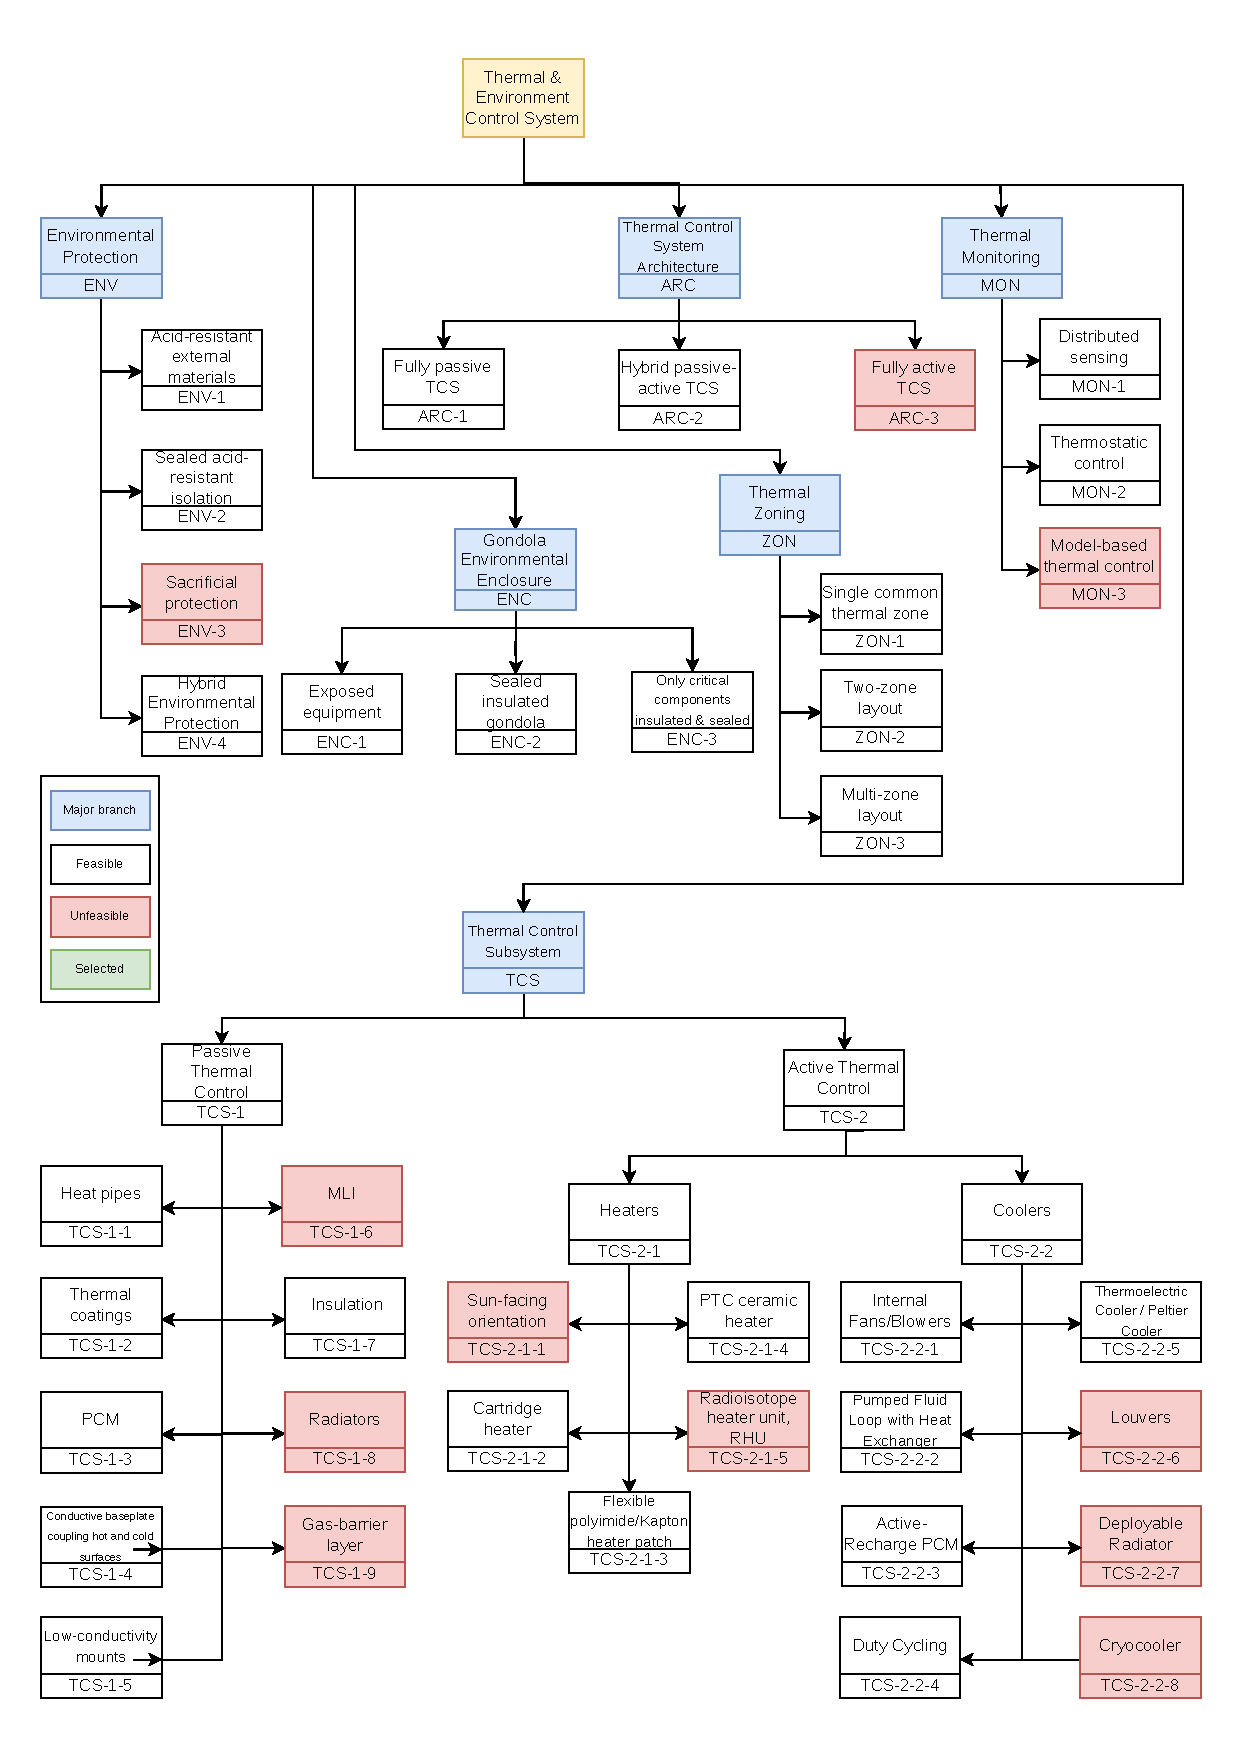
\includegraphics[width=1.0\linewidth]{fig/WFD-DOT_Th&Env.drawio.pdf}
    \caption{Thermal and environmental-control design option tree.}
    \label{fig:TCStreeplaceholder}
\end{figure}

\subsection*{Pruned Options}
\label{subsec:tcs_pruned_options}

The following options are removed before the trade-off procedure because they are incompatible with the constraints.

\begin{itemize}[itemsep=1pt, parsep=1pt]

\item \textbf{ARC-3 - Fully active TCS}: Rejected due to high mass, continuous power demand, and increased reliability risk compared with a passive-dominant hybrid architecture.

\item \textbf{ENV-3 - Sacrificial protection}: Rejected because degradation-based protection cannot guarantee stable environmental isolation over the full mission lifetime.

\item \textbf{MON-3 - Model-based thermal control}: Rejected at this stage because it requires a validated high-fidelity thermal model, more sensors, and more complex control logic.

\item \textbf{TCS-2-1-1 - Sun-facing orientation}: Rejected because the aerobot drifts with the Venus atmosphere and cannot rely on fixed orientation relative to the Sun.
\item \textbf{TCS-2-1-5 - Radioisotope heater unit, RHU}: Constant nuclear heating is not required and cannot be easily switched off. RHUs also introduce major safety, availability, integration, and regulatory constraints compared with simple electrical heaters.
\item \textbf{TCS-1-6 - MLI-based external insulation}: Rejected as primary external insulation because MLI is most effective in vacuum, while Venus atmospheric convection is expected to dominate heat transfer.

\item \textbf{TCS-2-2-6 - Louvers}: Rejected because external moving parts are difficult to seal and protect from sulfuric-acid aerosols over a long-duration mission.

\item \textbf{TCS-2-2-7 - Deployable radiator}: Rejected due to deployment risk, exposed moving interfaces, acid compatibility concerns, and limited heat-rejection benefit in the warm Venus atmosphere.

\item \textbf{TCS-2-2-8 - Cryocoolers}: Rejected because cryogenic temperatures are not required, and the mass, power demand, vibration, and complexity are not justified for ordinary electronics operating temperatures.

\end{itemize}
%------------------------------------------------------------------------
\section{Trade-Off}
\subsection{Trade-Off Method}

\label{sec:tcs_tradeoff_method}
Because the TCS consists of compatible hardware functions rather than one mutually exclusive architecture, the trade-off is performed in functional groups and then integrated into one selected concept. Architecture, enclosure, zoning, environmental protection, passive control, heating, and cooling options are compared separately using criteria relevant to each decision group.

A score from 1 to 5 is used for all trade-off criteria. A score of 1 indicates poor performance or major design risk, 3 indicates acceptable performance with concerns, and 5 indicates strong performance with low implementation risk.

\subsection{Candidate Architecture Tradeoffs}

\definecolor{score5}{RGB}{0,176,80}
\definecolor{score4}{RGB}{146,208,80}
\definecolor{score3}{RGB}{255,255,0}
\definecolor{score2}{RGB}{255,192,0}
\definecolor{score1}{RGB}{255,0,0}

% ============================================================
% ARCHITECTURE TRADE-OFF
% ============================================================

\subsection*{TCS method}

\begin{table}[H]
\centering
\normalsize
\caption{Thermal Control System architecture trade-off.}
\label{tab:tcs_architecture_tradeoff}
\renewcommand{\arraystretch}{1}
\setlength{\tabcolsep}{2pt}
\resizebox{\textwidth}{!}{%
\begin{tabular}{|p{1.3cm}|p{3.0cm}|p{4.0cm}|p{3.6cm}|p{3.6cm}|p{3.4cm}|p{3.6cm}|p{0.9cm}|}
\hline
\textbf{ID} &
\textbf{Option$\downarrow$ / Criteria$\rightarrow$} &
\textbf{Thermal Performance (30\%)} &
\textbf{Power Demand (25\%)} &
\textbf{Reliability (20\%)} &
\textbf{Mass / Complexity (15\%)} &
\textbf{Venus Environment Compatibility (10\%)} &
\textbf{Score} \\
\hline

ARC-1 &
\textbf{Fully passive TCS} &
\scorecell{2}{Limited control authority during hot and cold cases.} &
\scorecell{5}{No active thermal-control power required.} &
\scorecell{4}{Failure modes like surface degradation possible, but no moving parts.} &
\scorecell{5}{Lowest mass and simplest implementation.} &
\scorecell{1}{May not protect all sensitive hardware under harshest Venus conditions and throughout missions lifetime.} &
\textbf{3.5} \\
\hline

ARC-2 &
\textbf{Hybrid passive-active TCS} &
\scorecell{5}{Passive stability with local active correction where required.} &
\scorecell{3}{Active power needed only when required.} &
\scorecell{2}{Failure modes like surface degradation possible, but active elements can fail as well.} &
\scorecell{4}{Moderate mass and medium hardware count.} &
\scorecell{5}{Can adapt to Venus atmosphere variations and local component needs.} &
\textbf{3.75} \\
\hline

\end{tabular}%
}
\end{table}

% ============================================================
% GONDOLA ENCLOSURE TRADE-OFF
% ============================================================

\subsection*{Gondola Enclosure}
\begin{table}[H]
\centering
\normalsize
\caption{Gondola environmental enclosure trade-off.}
\label{tab:gondola_enclosure_tradeoff}
\renewcommand{\arraystretch}{1.25}
\setlength{\tabcolsep}{2pt}
\resizebox{\textwidth}{!}{%
\begin{tabular}{|p{1.3cm}|p{3.1cm}|p{4.4cm}|p{4.2cm}|p{3.8cm}|p{3.8cm}|p{0.9cm}|}
\hline
\textbf{ID} &
\textbf{Option$\downarrow$ / Criteria$\rightarrow$}&
\textbf{Environmental Isolation (35\%)} &
\textbf{Thermal Protection (35\%)} &
\textbf{Mass / Complexity (20\%)} &
\textbf{Integration, Simplicity (10\%)} &
\textbf{Score} \\
\hline

ENC-1 &
\textbf{Exposed equipment} &
\scorecell{1}{Sensitive equipment would be directly exposed to Venus atmosphere and acid aerosols.} &
\scorecell{1}{Poor protection from external convection and environmental temperature changes.} &
\scorecell{5}{Lowest mass and no enclosure hardware.} &
\scorecell{5}{Simple.} &
\textbf{2.2} \\
\hline

ENC-2 &
\textbf{Sealed, insulated gondola} &
\scorecell{5}{Protects electronics from sulfuric-acid aerosols and direct atmospheric exposure.} &
\scorecell{5}{Good protection from external convection and radiation changes.} &
\scorecell{2}{Biggest mass of shell, insulation, seals, and feedthroughs.} &
\scorecell{2}{Requires sealing, feedthroughs, and internal layout.} &
\textbf{4.1} \\
\hline

ENC-3 &
\textbf{Only critical components insulated and sealed} &
\scorecell{4}{Protects selected critical items only.} &
\scorecell{4}{Protects selected critical items only.} &
\scorecell{4}{Lower mass than a fully sealed gondola.} &
\scorecell{3}{Requires several local enclosures and interfaces.} &
\textbf{3.9} \\
\hline

\end{tabular}%
}
\end{table}

% ============================================================
% THERMAL ZONING TRADE-OFF
% ============================================================

\subsection*{Thermal Zoning}
\begin{table}[H]
\centering
\normalsize
\caption{Thermal zoning trade-off.}
\label{tab:thermal_zoning_tradeoff}
\renewcommand{\arraystretch}{1.25}
\setlength{\tabcolsep}{2pt}
\resizebox{\textwidth}{!}{%
\begin{tabular}{|p{1.3cm}|p{3.1cm}|p{4.4cm}|p{4.0cm}|p{3.8cm}|p{3.5cm}|p{0.9cm}|}
\hline
\textbf{ID} &
\textbf{Option$\downarrow$ / Criteria$\rightarrow$} &
\textbf{Component Thermal Compliance (35\%)} &
\textbf{Control (25\%)} &
\textbf{Mass / Complexity (30\%)} &
\textbf{Fault Isolation (10\%)} &
\textbf{Score} \\
\hline

ZON-1 &
\textbf{Single common thermal zone} &
\scorecell{3}{Assuming same temperature for all components results in more limiting and power demanding system, having to keep $\approx 40 ^\circ C$ .} &
\scorecell{1}{No ability to treat batteries, payload, avionics, and sampler separately.} &
\scorecell{5}{Simplest and lowest-mass layout.} &
\scorecell{3}{One local thermal issue can affect the full gondola interior.} & \textbf{}
\textbf{3.1} \\
\hline

ZON-2 &
\textbf{Two-zone layout} &
\scorecell{4}{Zones can be kept at two different temperatures, resulting in less power usage.} &
\scorecell{3}{Allows at least a warm electronics/battery zone and a payload/sampling zone.} &
\scorecell{4}{Good balance between performance and mass / complexity.} &
\scorecell{4}{Medium fault separation.} & \textbf{3.75}
\textbf{} \\
\hline

ZON-3 &
\textbf{Multi-zone layout} &
\scorecell{5}{Best ability to satisfy different component temperature limits.} &
\scorecell{5}{Highest flexibility for batteries, avionics, payload, sampling path, and external interfaces.} &
\scorecell{1}{Highest mass and complexity.} &
\scorecell{5}{Best containment of local faults.} & \textbf{3.80}
\textbf{} \\
\hline

\end{tabular}%
}
\end{table}

% ============================================================
% ENVIRONMENTAL PROTECTION TRADE-OFF
% ============================================================

\subsection*{Environmental Protection}

\begin{table}[H]
\centering
\normalsize
\caption{Environmental protection trade-off.}
\label{tab:environmental_protection_tradeoff}
\renewcommand{\arraystretch}{1.25}
\setlength{\tabcolsep}{2pt}
\resizebox{\textwidth}{!}{%
\begin{tabular}{|p{1.3cm}|p{3.3cm}|p{5.0cm}|p{4.2cm}|p{4.4cm}|p{0.9cm}|}
\hline
\textbf{ID} &
\textbf{Option$\downarrow$ / Criteria$\rightarrow$} &
\textbf{Acid Protection (50\%)} &
\textbf{Mass / Complexity (25\%)} &
\textbf{Integration, Simplicity (25\%)} &
\textbf{Score} \\
\hline

ENV-1 &
\textbf{Acid-resistant external materials} &
\scorecell{4}{Protects exposed surfaces if material compatibility is sufficient.} &
\scorecell{5}{Simple and lightweight compared with sealed or hybrid protection.} &
\scorecell{2}{Useful for exposed surfaces, but does not fully protect feedthroughs or sampling interfaces.} &
\textbf{3.75} \\
\hline

ENV-2 &
\textbf{Sealed acid-resistant isolation} &
\scorecell{4}{Strong protection for internal hardware if seals remain intact.} &
\scorecell{2}{Adds shell, sealings and feedthroughs.} &
\scorecell{3}{Works well for gondola electronics but requires careful inlet and feedthrough design.} &
\textbf{3.25} \\
\hline

ENV-4 &
\textbf{Hybrid environmental protection} &
\scorecell{5}{Combines sealed isolation with acid-resistant surfaces and local protection.} &
\scorecell{4}{Moderate mass and complexity penalty.} &
\scorecell{5}{Best compatibility with gondola, external shell, feedthroughs, and sampling path.} &
\textbf{4.75} \\
\hline

\end{tabular}%
}
\end{table}

%---------------------------------------------------------

\subsection{Candidate Active Heating and Cooling Options}
\label{sec:tcs_candidate_options}

The Thermal Control System is divided into three functional groups: passive thermal control, active heating options and active cooling options. Trade-offs are therefore performed for them separately. The final architecture is formed by combining the most suitable options.

\subsection*{Passive Thermal Control Options}
\label{subsec:passive_heating_options}

Passive thermal control options do not need electricity to operate. They can reduce fluctuations in temperature, temporarily store heat or redistribute it. These options are preferred where possible because they reduce power demand and improve long-duration reliability.

% ============================================================
% PASSIVE THERMAL CONTROL TRADE-OFF
% ============================================================

\begin{table}[H]
\centering
\normalsize
\caption{Passive thermal-control hardware trade-off.}
\label{tab:passive_thermal_control_tradeoff}
\renewcommand{\arraystretch}{1.25}
\setlength{\tabcolsep}{2pt}
\resizebox{\textwidth}{!}{%
\begin{tabular}{|p{1.5cm}|p{3.2cm}|p{4.5cm}|p{3.8cm}|p{3.8cm}|p{4.0cm}|p{1.0cm}|}
\hline
\textbf{ID} &
\textbf{Option$\downarrow$ / Criteria$\rightarrow$} &
\textbf{Thermal Usefulness (35\%)} &
\textbf{Mass / Complexity (20\%)} &
\textbf{Reliability (25\%)} &
\textbf{Venus Environment Compatibility (20\%)} &
\textbf{Score} \\
\hline

TCS-1-1 &
\textbf{Heat pipes} &
\scorecell{4}{Good heat-transport capability.} &
\scorecell{3}{More complex than straps or baseplates.} &
\scorecell{4}{Reliable if sealed inside gondola.} &
\scorecell{3}{Gravity and orientation have effect.} & \textbf{3.60}
\\
\hline

TCS-1-2 &
\textbf{Thermal coatings} &
\scorecell{5}{Can reduce solar absorption or improve heat rejection.} &
\scorecell{5}{Very low mass and simple to apply.} &
\scorecell{2}{No moving parts.} &
\scorecell{3}{Degradation, will most likely happen and must be considered.} & 3.85
\\
\hline

TCS-1-3 &
\textbf{PCM} &
\scorecell{3}{Buffers short hot or cold transients.} &
\scorecell{2}{Adds mass.} &
\scorecell{5}{Passive and reliable.} &
\scorecell{4}{Suitable inside sealed gondola.} & \textbf{3.5}
\\
\hline

TCS-1-4 &
\textbf{Conductive baseplate coupling hot and cold surfaces} &
\scorecell{4}{Spreads heat and allows waste-heat redistribution.} &
\scorecell{4}{Medium/low mass, not too hard to add.} &
\scorecell{5}{Highly reliable passive hardware.} &
\scorecell{5}{Protected inside gondola and compatible with Venus operation.} & \textbf{4.45}
\\
\hline

TCS-1-5 &
\textbf{Low-conductivity mounts} &
\scorecell{5}{Reduces unwanted heat leakage to/from external structure.} &
\scorecell{5}{Simple and medium/low mass.} &
\scorecell{5}{Passive and highly reliable.} &
\scorecell{5}{Useful for isolating components from external atmospheric swings.} & \textbf{5}
\\
\hline

TCS-1-7 &
\textbf{Insulation} &
\scorecell{5}{Reduces heat loss or heat ingress for critical zones.} &
\scorecell{3}{Medium mass, simple.} &
\scorecell{5}{Passive and reliable.} &
\scorecell{4}{Must be protected from atmospheric and acid exposure.} & \textbf{4.4}
\\
\hline



\end{tabular}%
}
\end{table}



\subsection*{Active Heating Options}
\label{subsec:active_heating_options}

Active heating options use electrical power or dedicated heat sources to raise component temperatures.

% ============================================================
% ACTIVE HEATING TRADE-OFF
% ============================================================

\begin{table}[H]
\centering
\normalsize
\caption{Active heating hardware trade-off.}
\label{tab:active_heating_tradeoff}
\renewcommand{\arraystretch}{1.25}
\setlength{\tabcolsep}{2pt}
\resizebox{\textwidth}{!}{%
\begin{tabular}{|p{1.9cm}|p{3.2cm}|p{4.0cm}|p{3.6cm}|p{3.8cm}|p{4.0cm}|p{0.9cm}|}
\hline
\textbf{ID} &
\textbf{Option$\downarrow$ / Criteria$\rightarrow$} &
\textbf{Heating Effectiveness (35\%)} &
\textbf{Power Demand (25\%)} &
\textbf{Reliability / Simplicity (20\%)} &
\textbf{Integration Suitability (20\%)} &
\textbf{Score} \\
\hline

TCS-2-1-2 &
\textbf{Cartridge heater} &
\scorecell{5}{Strong heating of chambers.} &
\scorecell{4}{Can require moderate power depending on target temperature.} &
\scorecell{5}{Simple resistive device.} &
\scorecell{3}{Best for chambers, not flat surfaces.} & \textbf{4.35}
\\
\hline

TCS-2-1-3 &
\textbf{Flexible polyimide/Kapton heater patch} &
\scorecell{5}{Direct and effective conversion of electrical power to heat.} &
\scorecell{4}{Power demand depends directly on required heat input.} &
\scorecell{5}{Simple, mature, and robust.} &
\scorecell{4}{Good for local heating of selected components.} & \textbf{4.55}
\\
\hline



TCS-2-1-4 &
\textbf{PTC ceramic heater} &
\scorecell{4}{Self-regulating heating, but less precise.} &
\scorecell{4}{Can reduce overheating risk and unnecessary power use.} &
\scorecell{3}{Simple, but space/environment compatibility must be verified.} &
\scorecell{3}{Useful for simple survival heating only.} & \textbf{3.60}
\\
\hline



\end{tabular}%
}
\end{table}


\subsection*{Active Cooling Options}
\label{subsec:active_cooling_options}

Active cooling options require electrical power or moving mechanisms to reduce component temperature or increase heat rejection. These options are useful when passive cooling is insufficient.

% ============================================================
% ACTIVE COOLING TRADE-OFF
% ============================================================

\begin{table}[H]
\centering
\normalsize
\caption{Active cooling and heat-load reduction trade-off.}
\label{tab:active_cooling_tradeoff}
\renewcommand{\arraystretch}{1.25}
\setlength{\tabcolsep}{2pt}
\resizebox{\textwidth}{!}{%
\begin{tabular}{|p{1.7cm}|p{3.2cm}|p{4.2cm}|p{3.6cm}|p{3.8cm}|p{4.0cm}|p{0.9cm}|}
\hline
\textbf{ID} &
\textbf{Option$\downarrow$ / Criteria$\rightarrow$} &
\textbf{Cooling / Heat-Reduction Effectiveness (35\%)} &
\textbf{Power Demand (25\%)} &
\textbf{Reliability (20\%)} &
\textbf{Integration Suitability (20\%)} &
\textbf{Score} \\
\hline

TCS-2-2-1 &
\textbf{Internal fans / blowers} &
\scorecell{3}{Reduces internal hot spots but does not reject heat by itself.} &
\scorecell{4}{Requires continuous or intermittent electrical power.} &
\scorecell{3}{Moving parts reduce long-duration reliability.} &
\scorecell{4}{Possible inside sealed gondola gas volume.} & \textbf{3.45}
\\
\hline

TCS-2-2-2 &
\textbf{Pumped fluid loop with heat exchanger} &
\scorecell{4}{High heat-transport capability.} &
\scorecell{3}{Requires pump power.} &
\scorecell{3}{Leakage and pump failure are risks.} &
\scorecell{3}{Higher mass and integration complexity.} & \textbf{3.35}
\\
\hline

TCS-2-2-3 &
\textbf{Active-recharge PCM} &
\scorecell{4}{Useful for repeated short-duration heat pulses.} &
\scorecell{3}{Requires pump power.} &
\scorecell{4}{Reliable if encapsulated and thermally cycled within limits.} &
\scorecell{3}{Higher mass and integration complexity.} & \textbf{3.55}
\\
\hline

TCS-2-2-5 &
\textbf{Thermoelectric cooler / Peltier cooler} &
\scorecell{5}{Can cool small precision instruments.} &
\scorecell{2}{Inefficient and increases total heat rejection demand.} &
\scorecell{5}{Good reliability.} &
\scorecell{4}{Suitable for local cooling, low mass.} & \textbf{4.05}
\\
\hline


TCS-2-2-4 &
\textbf{Duty cycling} &
\scorecell{5}{Directly reduces average internal heat generation.} &
\scorecell{5}{No extra power required.} &
\scorecell{5}{No additional hardware.} &
\scorecell{5}{Very suitable for measurements, communications, and ISRU scheduling.} & \textbf{5}
\\
\hline



\end{tabular}%
}
\end{table}

\section{Selected Thermal and Environmental Control Options}
\label{sec:selected_tcs_options}

The selected baseline is a sealed, insulated, two-zone gondola with hybrid environmental protection and mainly passive thermal control. Conductive baseplates, low-conductivity mounts, and insulation provide the primary thermal-control capability, reducing speed of temperature changes. Kapton heater patches are used for low-temperature-critical hardware, while thermoelectric coolers are used for local high-temperature-critical components. Duty cycling and altitude adjustment are used operationally to reduce thermal-control power demand. Selected options can be seen in \autoref{tab:selected_tcs_options}.

\small
\renewcommand{\arraystretch}{1.1}
\setlength{\tabcolsep}{3pt}

\begin{longtable}{|p{2.5cm}|p{3.4cm}|p{8.6cm}|}
\caption{Selected preliminary thermal and environmental-control options.}
\label{tab:selected_tcs_options}\\
\hline
\textbf{Decision Group} &
\textbf{Selected Option} &
\textbf{Reason for Selection} \\
\hline
\endfirsthead

\hline
\textbf{Decision Group} &
\textbf{Selected Option} &
\textbf{Reason for Selection} \\
\hline
\endhead

TCS architecture &
Hybrid passive-active TCS &
Combines passive thermal stability with local active control for critical components that cannot be maintained within limits passively. \\
\hline

Gondola enclosure &
Sealed, insulated gondola &
Provides environmental isolation from sulfuric-acid aerosols and reduces heat transfer between the Venus atmosphere and internal hardware. \\
\hline

Thermal zoning &
Two-zone layout &
Separates warmer avionics/battery hardware from payload or sampling hardware while avoiding the complexity of a full multi-zone system. \\
\hline

Environmental protection &
Hybrid environmental protection &
Combines sealed internal protection with acid-compatible exposed surfaces, feedthroughs, sensors, and sampling interfaces. \\
\hline

Passive thermal control &
Conductive baseplate, low-conductivity mounts, insulation &
The conductive baseplate redistributes internal waste heat, low-conductivity mounts reduce unwanted heat leakage, and insulation limits heat transfer through the gondola wall. \\
\hline

Active heating &
Flexible polyimide/Kapton heater patches &
Selected for local heating of low-temperature-critical hardware, especially batteries, payload units, valves, and sensitive internal components. \\
\hline

Active cooling &
Thermoelectric cooler / Peltier cooler &
Retained for local cooling of high-temperature-critical hardware only, not for whole-gondola cooling. \\
\hline

Heat-load reduction &
Duty cycling  &
Applied to payload, communication, ISRU, and other powered subsystems to reduce average internal heat generation. \\
\hline

Heat-load reduction &
Altitude Control  &
Adjust external temperature by inflating or deflating the balloon. \\
\hline

\end{longtable}

\normalsize



\section{TCS Verification and Validation Plan}
\label{sec:tcs_vv}

The selected TCS concept is verified by analysis, inspection, and representative testing. The plan checks requirement compliance for thermal control, environmental protection, and the preliminary thermal model. Detailed facilities, durations, and margins will be refined in the final design phase.

\small
\renewcommand{\arraystretch}{1.12}
\setlength{\tabcolsep}{3pt}

\begin{longtable}{|p{2.4cm}|p{2.8cm}|p{5.0cm}|p{5.0cm}|}
\caption{Preliminary TCS verification approach.}
\label{tab:tcs_verification}\\
\hline
\textbf{Requirement} &
\textbf{Verification Method} &
\textbf{Planned Activity} &
\textbf{Acceptance Criterion} \\
\hline
\endfirsthead

\hline
\textbf{Requirement} &
\textbf{Verification Method} &
\textbf{Planned Activity} &
\textbf{Acceptance Criterion} \\
\hline
\endhead

REQ-TCS-01 &
Analysis and test &
Build a lumped thermal model and evaluate survival temperatures for hot, cold, safe-mode, and non-operational cases. Correlate with representative thermal-balance testing. &
All critical components remain within survival limits and show positive thermal margin after model correlation. \\
\hline

REQ-TCS-02 &
Analysis and test &
Evaluate operational temperatures for batteries, avionics, payload instruments, and sampling hardware using subsystem heat dissipation and control modes. &
All operating components remain within operational limits, or have a defined duty-cycle or thermal-control mode. \\
\hline

REQ-TCS-04 &
Material test and inspection &
Expose representative coatings, seals, feedthroughs, insulation barriers, and external materials to sulfuric-acid aerosol conditions and thermal cycling. &
No unacceptable cracking, leakage, delamination, or loss of sealing, structural, or thermal-control function. \\
\hline

REQ-TCS-05 &
Inspection and functional test &
Inspect sensor placement and verify temperature telemetry during hot/cold testing and heater/cooler activation. &
All required thermal zones provide valid telemetry and support the intended control actions. \\
\hline

REQ-ENV-01 &
Material test and inspection &
Test external surfaces, coatings, feedthroughs, and exposed interfaces under representative acid exposure. &
Exposed materials remain compatible with sulfuric-acid aerosols and retain their intended function. \\
\hline

REQ-ENV-02 &
Leak test and inspection &
Inspect sealed gondola interfaces, feedthroughs, and sampling-line penetrations. Perform leak testing before and after thermal cycling. &
Protected electronics, batteries, avionics, and payload hardware remain isolated from direct Venus atmospheric exposure. Leak rates remain below the detailed-design limit. \\
\hline

REQ-ENV-03 &
Analysis and material test &
Check environmental-protection materials against the expected thermal range and test samples through thermal cycling. &
Materials show no unacceptable loss of sealing, adhesion, or mechanical function over the expected thermal range. \\
\hline

TCS model and tool V\&V &
Independent calculation &
Compare thermal-model outputs with hand calculations for wall heat leak, heater power, cooling power, and heat rejection. &
Model results are physically consistent with simplified analytical calculations, or differences are explained by documented assumptions. \\
\hline

\end{longtable}

\normalsize
\section{Sensitivity Analysis}
\label{sec:tcs_sensitivity}

A preliminary sensitivity analysis is performed qualitatively because the detailed thermal model is not yet available. The selected architecture is mainly sensitive to insulation conductivity, insulation thickness, heat-leak safety factor, internal power dissipation, and cooler COP. The trade-off outcome is not expected to change for small variations in passive hardware scores, because insulation, low-conductivity mounts, and conductive baseplates remain low-power and high-reliability options. However, if internal heat generation is significantly higher than expected, local active cooling or stronger duty cycling may become more important.

The architecture trade-off is most sensitive to the power-demand and reliability criteria. If power demand is weighted more strongly, the fully passive option becomes more competitive, but it still lacks sufficient control authority for critical components. If thermal performance is weighted more strongly, the hybrid passive-active architecture remains preferred.

\begin{table}[H]
\centering
\caption{Preliminary architecture trade-off sensitivity cases.}
\label{tab:tcs_sensitivity_cases}
\begin{tabular}{|p{4.2cm}|p{4.0cm}|p{5.0cm}|}
\hline
\textbf{Sensitivity case} & \textbf{Observed effect} & \textbf{Conclusion} \\
\hline
Power-demand weight increased by 10\% & ARC-1 becomes closer to ARC-2 & Hybrid selection remains preferred because ARC-1 lacks local control authority. \\
\hline
Reliability weight increased by 10\% & ARC-1 becomes closer to ARC-2 & Requires reliability justification for active elements. \\
\hline
Venus compatibility criterion removed & ARC-2 advantage decreases & Environmental adaptability is a driver of the hybrid concept. \\
\hline
ARC-2 reliability score reduced from 2 to 1 & ARC-2 margin becomes small & Active elements must be simple, redundant, or non-critical. \\
\hline
Hot-case heat leak doubled from 40 W to 80 W & Local cooling and duty cycling become more important & Detailed thermal model required before final design. \\
\hline
\end{tabular}
\end{table}

% \section{Protection from Sulfuric Acid Environment}
% \label{sec:protection_sulfuric_acid}

% The selected environmental protection concept is hybrid: sensitive hardware is kept inside the sealed insulated gondola, while exposed surfaces, feedthroughs, sensors, and sampling interfaces use acid-compatible materials. Aerosol inlets and sampling lines are treated as high-risk interfaces because they intentionally contact the Venus atmosphere.
% The preliminary environmental protection stack for the gondola is shown in \autoref{tab:env_material_stack}.

% \begin{table}[H]
% \centering
% \caption{Preliminary environmental protection material stack.}
% \label{tab:env_material_stack}
% \renewcommand{\arraystretch}{1.15}
% \begin{tabular}{|p{3.2cm}|p{4.5cm}|p{5.8cm}|}
% \hline
% \textbf{Layer / Interface} &
% \textbf{Candidate Materials} &
% \textbf{Purpose} \\
% \hline

% Outer acid barrier &
% FEP, PTFE, PFA fluoropolymer film or coating &
% Provides direct protection against sulfuric-acid aerosols and reduces degradation of the structural shell. \\
% \hline

% Reflective thermal layer &
% Aluminized or silvered layer beneath transparent FEP/PFA &
% Reduces absorbed solar radiation while keeping the reflective layer protected from acid exposure. \\
% \hline

% Structural shell &
% Titanium alloy, stainless steel, protected aluminium, or corrosion-resistant alloy &
% Provides mechanical strength and supports feedthroughs, mounting points, and enclosure sealing. \\
% \hline

% Insulation layer &
% Aerogel blanket, microporous silica, or protected foam insulation &
% Reduces heat transfer between the external shell and internal gondola volume. This layer is not directly exposed to acid aerosols. \\
% \hline

% Internal liner / baseplate &
% Aluminium or other thermally conductive internal structure &
% Provides mounting support and internal heat spreading for avionics, payload, and power hardware. \\
% \hline

% Seals and feedthroughs &
% Metal seals, ceramic-to-metal feedthroughs, glass-to-metal feedthroughs, PTFE/PFA-compatible seals &
% Maintains environmental isolation between the Venus atmosphere and internal gondola volume. \\
% \hline

% Sampling path &
% PFA/PTFE-lined tubing, titanium, Hastelloy-type fittings, acid-compatible valve materials &
% Allows controlled atmospheric sampling while preventing contamination of the main gondola volume. \\
% \hline

% \end{tabular}
% \end{table}

% Use acid-resistant materials as the first protection layer and to verify their long-duration compatibility through environmental testing.

% Special attention is required for feedthroughs, sampling interfaces, valves, and external sensors. These are more critical than the flat shell surface because they create possible leakage paths into the gondola. Therefore, the sampling path shall be isolated from the main avionics bay, and any gas or aerosol path entering the vehicle shall include compatible materials, local sealing, and contamination-control measures.

% For the preliminary design, the baseline environmental protection concept is therefore:
% \begin{itemize}[itemsep=1pt, parsep=1pt]
%     \item acid-resistant external fluoropolymer protection on exposed gondola surfaces;
%     \item sealed isolation of sensitive electronics, batteries, avionics, and most payload hardware;
%     \item protected internal insulation that is not directly exposed to acid aerosols;
%     \item acid-compatible feedthroughs, seals, sampling tubes, and valve interfaces;
%     \item separate environmental treatment of the aerosol sampling path;
%     \item environmental compatibility testing of all exposed materials and thermal surfaces.
% \end{itemize}





The preliminary Thermal and Environmental Control Subsystem is a hybrid system with passive methods dominating. A sealed and insulated gondola is selected to protect sensitive hardware from the Venus atmosphere, while low-conductivity mounts, insulation, and conductive baseplates provide the main thermal-control capability. Local heaters are used for batteries and some scientific instruments. Local thermoelectric cooling is implemented only as a backup for batteries and precision payload needs. The design shall be refined using detailed subsystem heat dissipation values, component datasheets, thermal bridge estimates, and environmental compatibility testing.
\chapter{Guidance \& Navigation}
\label{chapter: guidance and navigation}


\section{Tasks and goals}
\label{sec: tasks and goals}
Classically, the Guidance \& Navigation subsystem handles locating the spacecraft in 3D space, tracks the position history, predicts and plans trajectory, and computes commands for the propulsion subsystem required to maintain the trajectory. The GNS must provide this functionality starting at separation from the cruise stage and ending at atmospheric entry. During the entry, navigation subsystem keeps track of position, altitude, velocity, and provides this information to the deployment subsystem to stage the entry procedures.

For the nominal VISTA mission, the task fundamentally boils down just to position tracking. Active control of horizontal position would require countering the winds, which at 55 km altitude reach up to 60 m/s.

Since the balloon follows with winds that reach up to 60 m/s (at 55 km altitude), active position control in the horizontal direction is unfeasible. Altitude control through the buoyancy/weight balance is possible, and necessary to allow for conducting scientific investigation at different altitudes or to counter disturbance from vertical winds (up to a few meters per second).

\section{Design options}
\label{sec: design options}

The main challenge of navigating around Venus is the scarcity of absolute position measurements. Since the thick cloud layer completely diffuses incoming sunlight and Venus doesn't have an intrinsic magnetic field, the only available references are the Venusian surface and telecommunications with orbiters or Earth.

\begin{figure}[H]
    \centering
    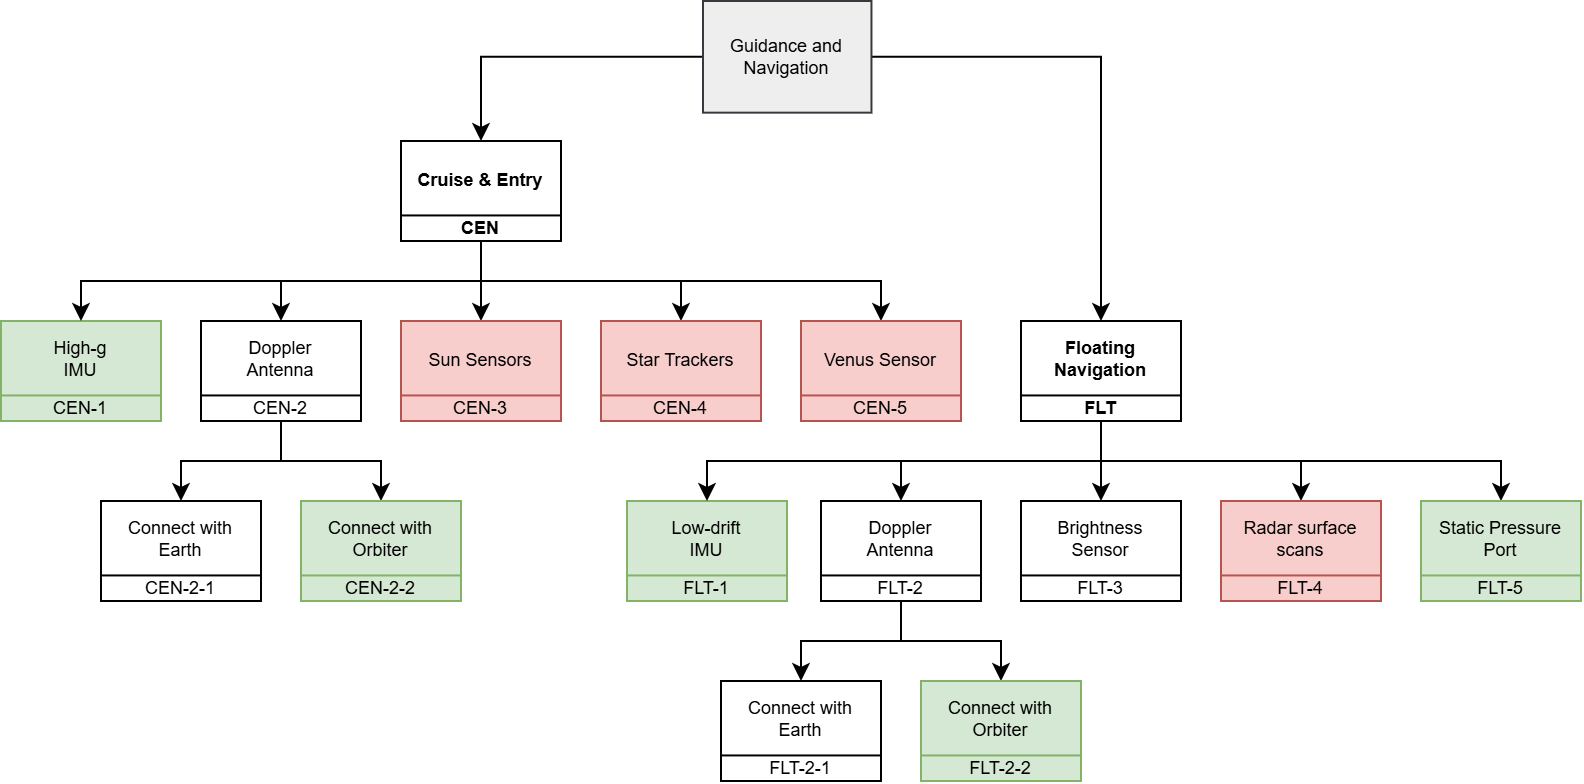
\includegraphics[width=\linewidth]{fig/DOT_navigation.png}
    \caption{Design Option Tree of the Guidance \& Navigation Subsystem}
    \label{fig: dot navigation}
\end{figure}

For the cruise and entry stage, the selected methods of navigation include Doppler antenna tracking with respect to the orbiter and propagation with a high-g inertial measurement unit. Conventional spacecraft strategies like sun senors or star trackers are not selected, since they involve dedicated equipment that only needs to operate for a few hours and is later discarded, which is very cost and mass inefficient.

During the nominal mission, balloon altitude can be easily determined by using a static pressure port and comparing to the reference atmosphere. In case no barometers are available in payload, a dedicated one will be necessary. The two methods of absolute determination of geographic coordinates are Doppler antenna tracking and radar surface imaging. Radar imaging is deemed unfeasible to due great mass and power requirements. Doppler tracking is designed to operate between the balloon and the relay orbiter. While tracking directly from Earth is possible, and has been done for the Vega missions, it would require dedicated time of the deep-space communication network, provides very poor data rates and only works for half the time due to Venus occlusion. It is not considered for nominal operation.

Since active control of the aerobot's geographic coordinates is not considered, real-time knowledge of position isn't critically necessary. Inertial measurements of the path can provide a convenient position estimation at times when the communication with the orbiter is not available, but are limited by the drift rate of the inertial sensors. Post-facto knowledge of absolute position and attitude measurements is a far easier task. As shown by \cite{Frazier2022}, the drift errors of the IMUs can be anchored at the beginning and end of the communications blackout period, which effectively halves the total drift period.  

\begin{figure}[H]
    \centering
    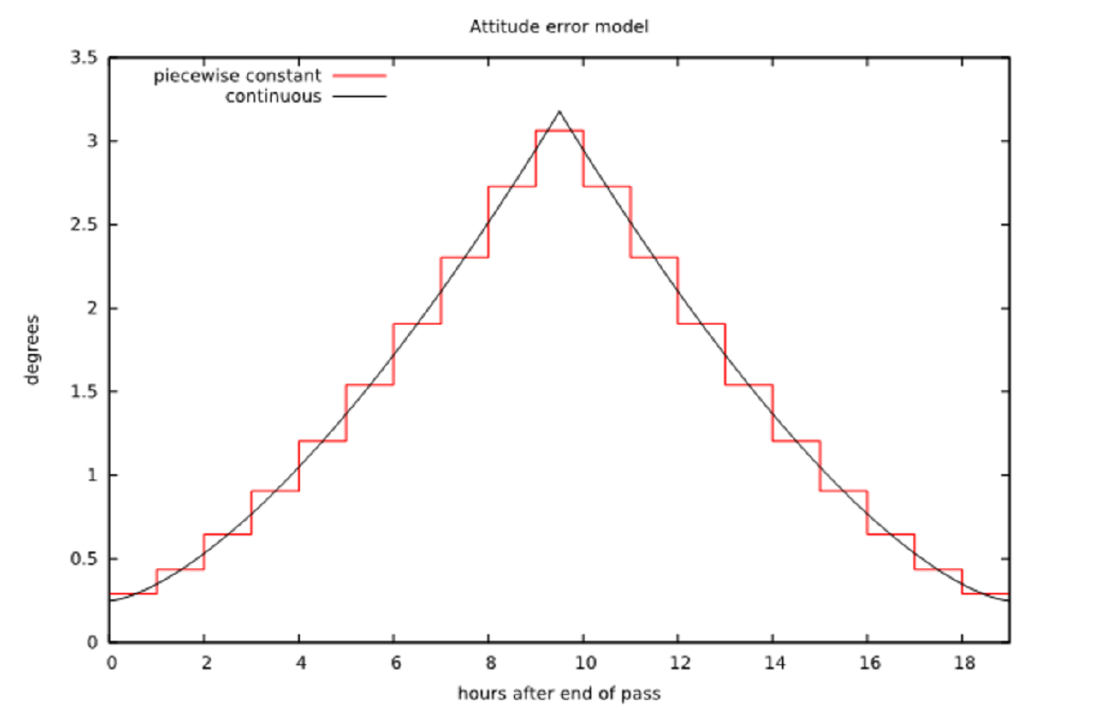
\includegraphics[width=0.75\linewidth]{fig/IMU_drift.png}
    \caption{Attitude error modeling during a tracking gap \cite{Frazier2022}}
    \label{fig: imu drift}
\end{figure}

\section{Hardware components}
\label{sec: hardware components}

The navigation subsystem is a bit unique, in a sense it is primarily software-based, and all hardware required by it is used by other subsystems. The main purpose of the antenna used for Doppler tracking is as a communications relay, the IMUs are mostly considered for ADCS, and the barometers are part of payload. The mass and power of these elements is included in the budgets of the corresponding subsystems. For convenience, it is also summarized in \autoref{tab: navigation hardware components} below. Notice that when operating, the IMUs necessarily require a 100\% duty cycle. A break in IMU tracking would introduce unknown and indeterminable deviations and make path reconstruction impossible. The pressure probe can have a very slow duty cycle. Brief measurements a few times per minute should be enough for good altitude tracking, since the balloon system altitude change is comparatively quite slow. It is important to have a data source acting as the official arbiter of daytime/nighttime determination. This can potentially be inferred from the working of the solar panels, or from payload instruments like a nephelometer or a camera. If such functionality cannot be easily and reliably provided by other subsystems, a dedicated ambient light intensity sensor should be installed.


\begin{table}[H]
\centering
\caption{Guidance \& Navigation Subsystem Components}
\label{tab: navigation hardware components}
\resizebox{\textwidth}{!}{%
\begin{tabular}{llllll}
\hline
\textbf{Component} &
  \textbf{Example Model} &
  \textbf{Power {[}W{]}} &
  \textbf{Duty Cycle {[}\%{]}} &
  \textbf{Mass {[}kg{]}} &
  \textbf{Avg. Power {[}W{]}}\\ \hline
Communications Antenna  & See Communications Subsystem      & 8              & 25\%                                       & \textless{}0.300 & 2       \\
High-g IMU              & GuideNav GUIDE 600G               & 2 (estimated)  & 100\% (cruise and entry only)              & 0.050            & 2       \\
Low-drift accelerometer & 3 x Honeywell single axis QA-3000 & 1.5            & 100\%                                      & 0.210            & 1.5     \\
Low-drift gyroscope     & Safran STIM300                    & 1.5            & 100\%                                      & 0.055            & 1.5     \\
Static Pressure Probe   & See Payload                       & \textless{}0.1 & 10\%                                       & \textless{}0.010 & $\sim$0 \\ \hline
                        &                                   &                & \textbf{Total}                             & $\sim$0.425      & 7      
\end{tabular}%
}
\end{table}

\section{Software components}
\label{software components}

During nominal operation, the Guidance and Navigation subsystem has two primary operational tasks: acquiring and storing tracking data from on-board sensors (\autoref{fig: nav flow 1}), and using the Doppler effects of the radio connection with the antenna to estimate absolute location and attitude (\autoref{fig: nav flow 2}). The GNS also cooperates with the buoyancy and nitrogen extraction subsystem to monitor and control the aerobot altitude (\autoref{fig: nav flow 3}).

\begin{figure}[H]
    \centering
    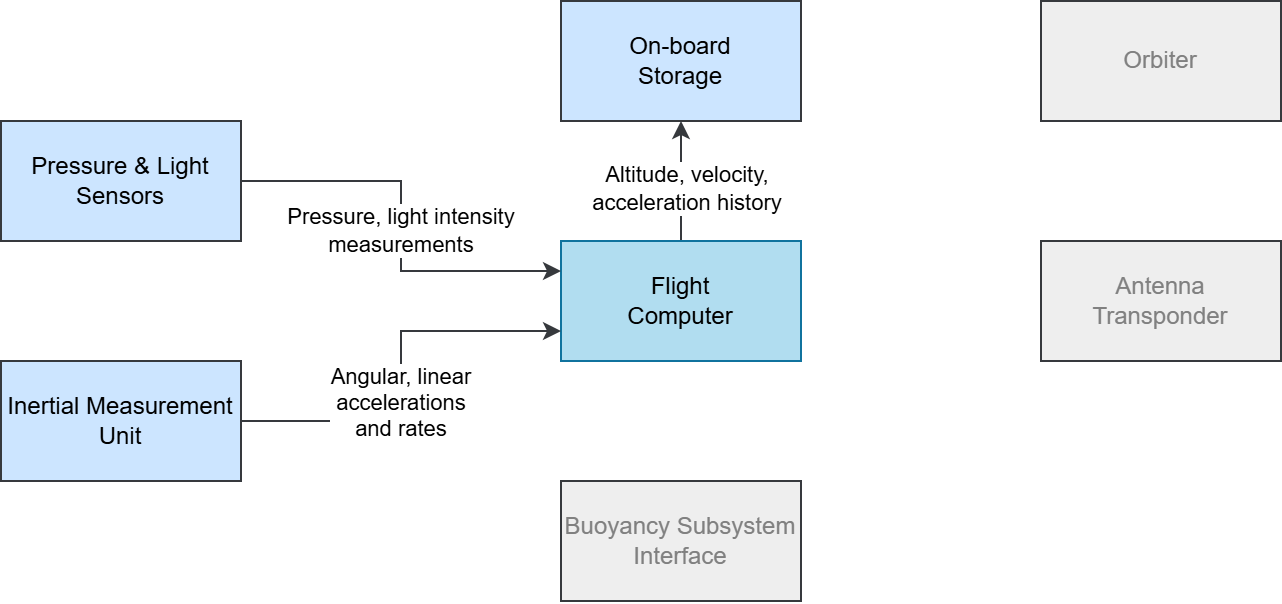
\includegraphics[width=0.85\linewidth]{fig/navigation_flow_1.png}
    \caption{GNS data flow of measurement acquisition}
    \label{fig: nav flow 1}
\end{figure}

During measurement acquisition, which keeps occurring throughout the nominal mission, the flight computer periodically samples the static pressure sensor (and the ambient light intensity sensor, if available). The inertial measurement unit runs continuously. The information about position and accelerations is logged and stored as telemetry for later use.

\begin{figure}[H]
    \centering
    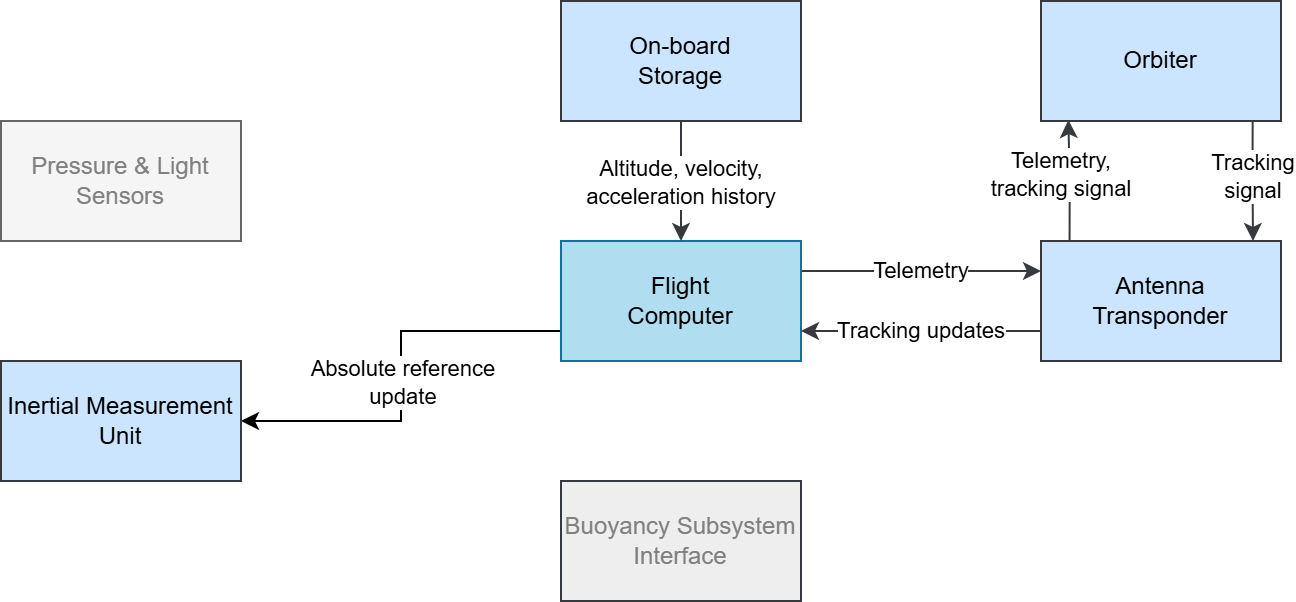
\includegraphics[width=0.85\linewidth]{fig/navigation_flow_2.png}
    \caption{GNS data flow during active Doppler ranging}
    \label{fig: nav flow 2}
\end{figure}

Active Doppler ranging is an operation mode that can only be active when the communication window to the orbiter is open and there is sufficient power available (it might be unfeasible to run this mode at night). During the transmission of standard telemetry or scientific data, the exact signal signature is studied to determine the distance between the aerobot and the orbiter (range), as well as the velocity and attitude change of the aerobot (range rate). If necessary for the procedure, a dedicated tracking signal will be transmitted instead. Using the tracking data, the absolute reference for the IMU can be updated.

\begin{figure}[H]
    \centering
    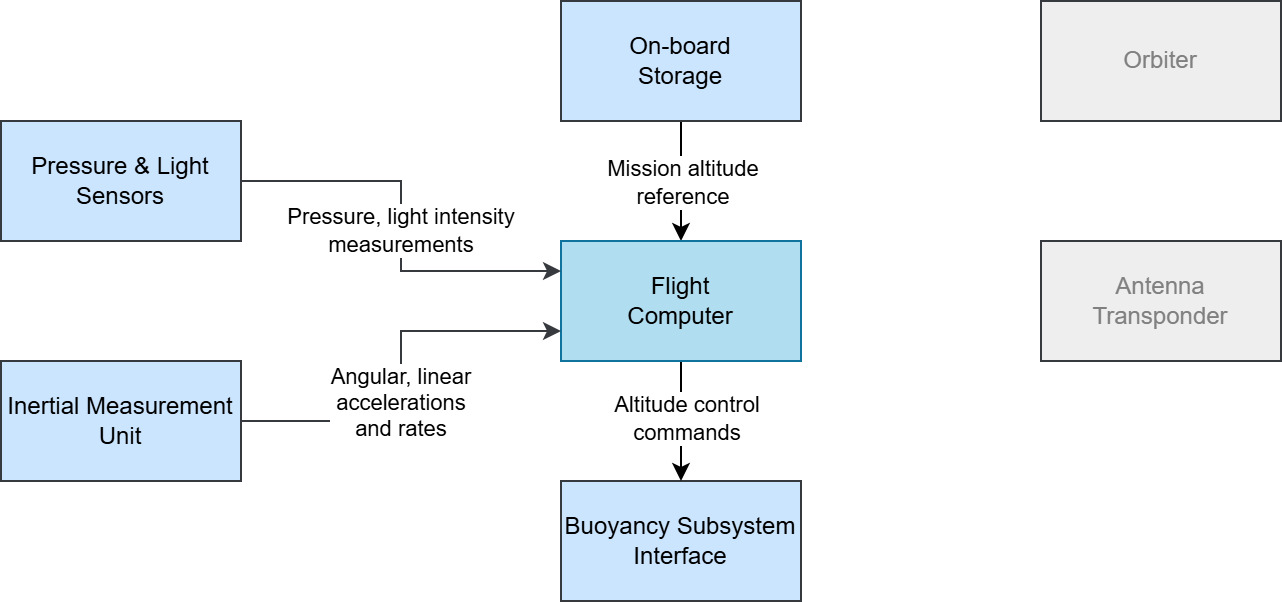
\includegraphics[width=0.85\linewidth]{fig/navigation_flow_3.png}
    \caption{GNS data flow during altitude control}
    \label{fig: nav flow 3}
\end{figure}

The GNS monitors and controls altitude continuously. The measured state is compared to a reference derived based on scientific targets and mission planning. The altitude control command is computed and sent to the buoyancy subsystem. The exact abstraction level of the navigation controller interface with the buoyancy subsystem code is undecided at this stage. A promising design for a model predictive altitude controller is given in \cite{apostol2025}, and is based on sequential convex programming for repeatedly approximating nonlinear aerobot dynamics.

\section{Navigation Verification and Validation}
The VISTA Mission would be the first one to deploy a Venus aerobot with long-term tracking abilities and altitude control. Its navigation subsystem mostly relies on software procedures and interacts with large scale Venusian weather, which is largely not understood. As such, conclusively proving accurate and reliable functioning is not feasible. Verification and validation efforts should focus on general robustness and ability to retain some functionality in many environments.

Extensive software verification shall be conducted to guarantee internal consistency and predictability. The behaviour of the navigation subsystem shall be investigated through simulation using atmospheric models (e.g. the Venus Climate Database \cite{VenusClimateDatabase}). Given the mission timeline, it should be possible to develop a dedicated climate model designed specifically for aerobot position propagation. The simulations should encompass a wide range of atmosphere input variables, to hopefully contain within itself the actual conditions that will be encountered durin the nominal mission.


\chapter{Power Subsystem}
\label{chap:power}

\noindent The Electrical Power Subsystem (EPS) is responsible for the generation, storage, distribution, and regulation of power within the aerobot. Initially, a power budget was constructed (that was re-iterated along with the sizing of the other subsystems). Using the power budget several options were considered to meet the power requirements for VISTA, some in more detail than others. After the selection of a particular EPS system was complete, a final list of EPS requirements was created, as well as an architecture diagram to visualize it clearly\footnote{Note that although the sections here are presented in a linear fashion, the process of designing the power subsystem involved overlapping between tasks and going back to re-evaluate on design choices based on conclusions drawn from latter sections. }.

\section{EPS Functionalities and Design Process}

Before starting the preliminary sizing of the EPS, some typical top-level functions were identified from SMAD \cite{wertz1999smad}. These are presented in the list below; the EPS
\begin{itemize}[itemsep=1pt, parsep=1pt]
    \item supplies a continuous source of electrical power to subsystem loads during the mission life.
    \item controls and distributes electrical power to the aerobot
    \item supports power requirements for average and peak electrical load.
    \item provides converters for ac and regulated dc power buses, if required.
    \item provides command and telemetry capability for EPS health and status, as well as control capability through the ground station or an autonomous system.
    \item protects the aerobot payload against failures within the EPS.
    \item suppresses transient bus voltages and protects against bus faults.
\end{itemize}

\noindent Sequentially, the preliminary design process is outlined in \ref{tab:eps-process}.


\begin{table}[H]
    \centering
    \caption{Preliminary design process for the EPS subsystem.}
    \label{tab:eps-process}
    \small
    \renewcommand{\arraystretch}{1.05}
    \setlength{\tabcolsep}{4pt}
    \begin{tabularx}{\textwidth}{@{}
        >{\centering\arraybackslash}p{0.15\textwidth}
        >{\RaggedRight\arraybackslash}p{0.15\textwidth}
        >{\RaggedRight\arraybackslash}p{0.28\textwidth}
        >{\RaggedRight\arraybackslash}X
    @{}}
        \toprule
        \textbf{\shortstack{Step\\Number}} & \textbf{Step Name} & \textbf{Inputs} & \textbf{Outputs} \\
        \midrule
        1 & Identify requirements & Top level requirements; mission type; spacecraft configuration; mission life; payload definition & Design requirements; spacecraft electrical power profile (average and peak) \\
        2 & Select and size power source & Outputs from step 1 & EOL power requirement; initial sizing (e.g.\ mass, area, type) of chosen power source \\
        3 & Select and size energy storage & Outputs from step 1 and step 2 & Eclipse and load leveling energy storage requirement; storage mass volume; storage type \\
        4 & Identify power regulation and control & Outputs from step 1 & Peak-power tracker or direct-energy-transfer system \\
        \bottomrule
    \end{tabularx}
\end{table}


\section{Power Bugdet and Modes}




\section{Power Source Design Options}

\autoref{fig:eps-tree} presents the initial design options considered as the power source for the EPS. 

\begin{figure}[H]
    \centering
    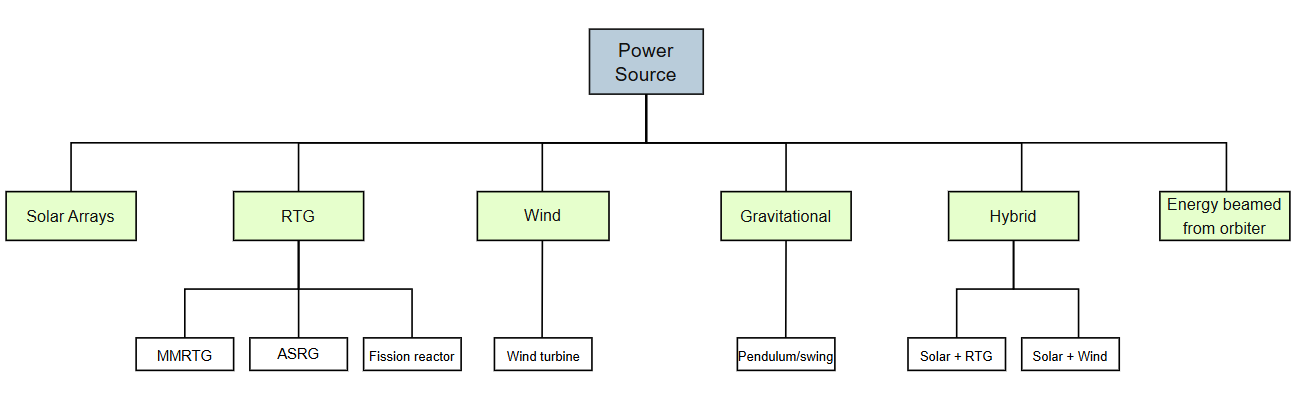
\includegraphics[width=\linewidth]{fig/eps-tree.png}
    \caption{Design option tree for the EPS}
    \label{fig:eps-tree}
\end{figure}

Some of these options can already be disregarded intuitively, without needing to carry out any further analysis or trade-off process. 

The \textbf{wind turbine}, which would have to be attached to a tether, needs relative motion between itself and the wind. Since the balloon is moving with the wind, the relative motion of the turbine to the wind is negligible, and thus no energy can be generated.

For the \textbf{swinigng pendulum}, the potential energy that can be generated is also essentially negligible, so it can not be considered neither as a primary nor backup power source.

Finally, the severe attenuation and cloud coverage variability make the \textbf{energy beamed from orbiter} very unreliable. Furthermore, energy can only be generated during the aerobot's contact windows with the orbiter, which would make random peak power demands very difficult to handle.

\section{Preliminary Sizing}
For the remaining power sources, a preliminary sizing of their energy capacity, mass, and cost is carried out. For the power sources that require a separate energy storage unit - this is considered later in \autoref{sub:energy-storage}. Some preliminary choices are also made for the power regulation and distribution system, although choices have pretty much been standardized for small spacecraft by ESA.
\subsection{Power Source}
For the preliminary sizing of the power generation systems, the general framework from SMAD is used to calculate the maximum power that needs to be generated at one instant:

\begin{equation}
    P_{sa} = \frac{\frac{P_{e}T_{e}}{X_{e}}+\frac{P_{d}T_{d}}{X_{d}}}{T_{d}}    
\end{equation}

where $P_{e}$ is the max power needed at night, $T_{e}$ the maximum amount of time the aerobot can spend at night, and $X_{e}$ is solar array-battery-load electrical path efficiency.  Furthermore, $P_{d}$ is the peak power demand during the day, $T_{d}$ is the maximum potential time spent in daylight, and $X_{d}$ is the solar-load electrical path efficiency\footnote{In actuality, the efficiency values for night and daylight depend on the type of power regulation method used - a conservative value is taken here.}.

The power values are taken from the power modes and the rest of the values are taken from literature.

\begin{align*}
    P_{sa} &= \frac{\frac{(10.65)(4 \hspace{1mm} \text{days})}{0.65}+\frac{(268.62)(4 \hspace{1mm} \text{days})}{0.85}}{4 \hspace{1mm} \text{days}}\\
    P_{sa} &= 331.915 \hspace{1mm} [W]
\end{align*}

\subsubsection{Solar Arrays}
Before proceeding with the sizing of the solar arrays, it is assumed that they are mounted on the ``free'' edges of the gondola (see \autoref{fig: solar-panels} - specific geometrical shape does not really matter at this stage, but is assumed to be cylindrical.

\begin{wrapfigure}{r}{0.2\textwidth}
    \centering
    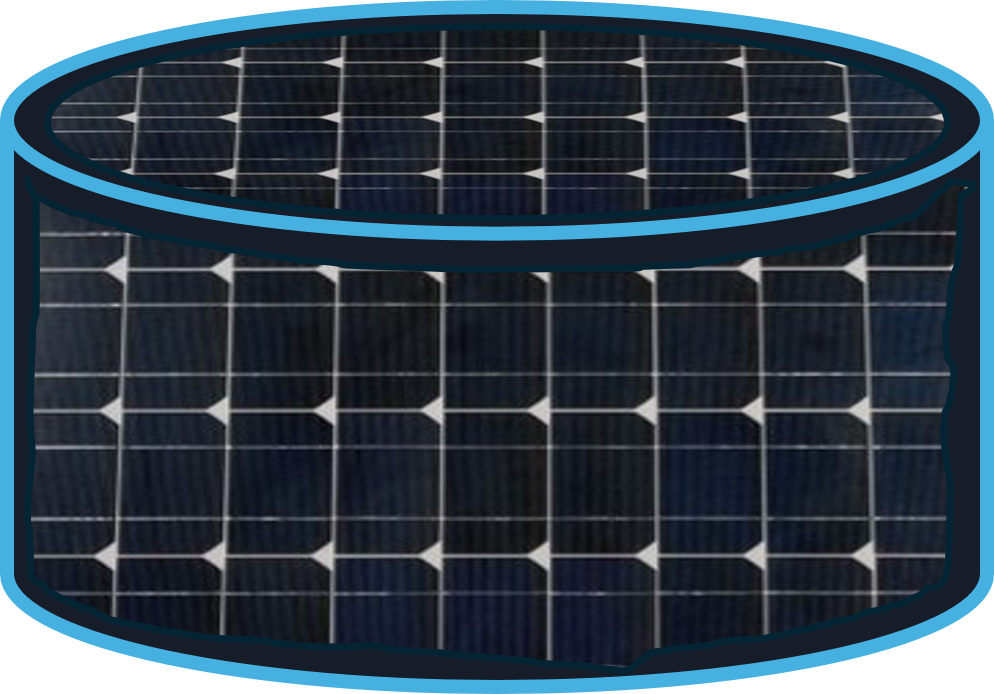
\includegraphics[width=0.2\textwidth]{Gondola-Panel-Pic.png}
    \caption{Enter Caption}
    \label{fig:placeholder}
\end{wrapfigure}


Now, one of the most important aspects of the design of the solar arrays, is calculating their potential solar power output based on the incoming solar flux. Landis carries out this procedure in \cite{}\footnote{Note that for the polar region, since the sun is never near zenith, the calculation is not applicable.}. The final output is the specific power [$W/m^{2}$] of a triple-junction solar cell as a function of altitude above the Venus datum. 

Before using his results however, two correction factors have to applied. Firstly, the ``shadowing effect'' from the aerobot's balloon has to be calculated, and secondly, a 5\% reduction in solar power output is applied due to the material coating that will applied to the solar cells to make them Venus environment resistant \cite{}.

\subsubsection*{Shadowing Effects}
There are three distinct shadowing effects that affect incident solar radiation to the solar arrays.
\begin{enumerate}
    \item Self-shadowing of the gondola by the balloon envelope.
    \item Self-shadowing within the gondola
    \item Cloud shadowing
\end{enumerate}

The latter is taken care of by Landis in \cite{}, while the second is ignored since it is assumed that the solar arrays will be attached on the edges of the gondola, so there will not be a shadow casted on them from the gondola.

For the self-shadowing of the gondola by the balloon envelope - the Sun-direction vector projects the balloon's silhouette onto the plane of the gondola. Whether the gondola is in the balloon's shadow depend on:
\begin{itemize}
    \item Solar zenith angle, $\theta_{z} (0^{o}$ -sun directly overhead, and $90^{o}$ - sun on the horizon)
    \item Tether length, $l$
    \item Balloon radius, $R_{b}$
    \item Gondola radius, $R_{g}$
    \item Horizontal offset between balloon center and gondola center, $s_{h}$ - assumed zero\footnote{This is conservative, as any non-zero value would mean the gondola is moving towards outside the balloon's shadow.}
\end{itemize}

The problem is treated in the 2D plane as the intersection between two circles. Note that in reality the shadow of the balloon on the gondola is probably some sort of ellipse, and the gondola shape is unknown, but a circular shape is used because it simplified the problem.

\begin{wrapfigure}{l}{0.45\textwidth}
    \centering
    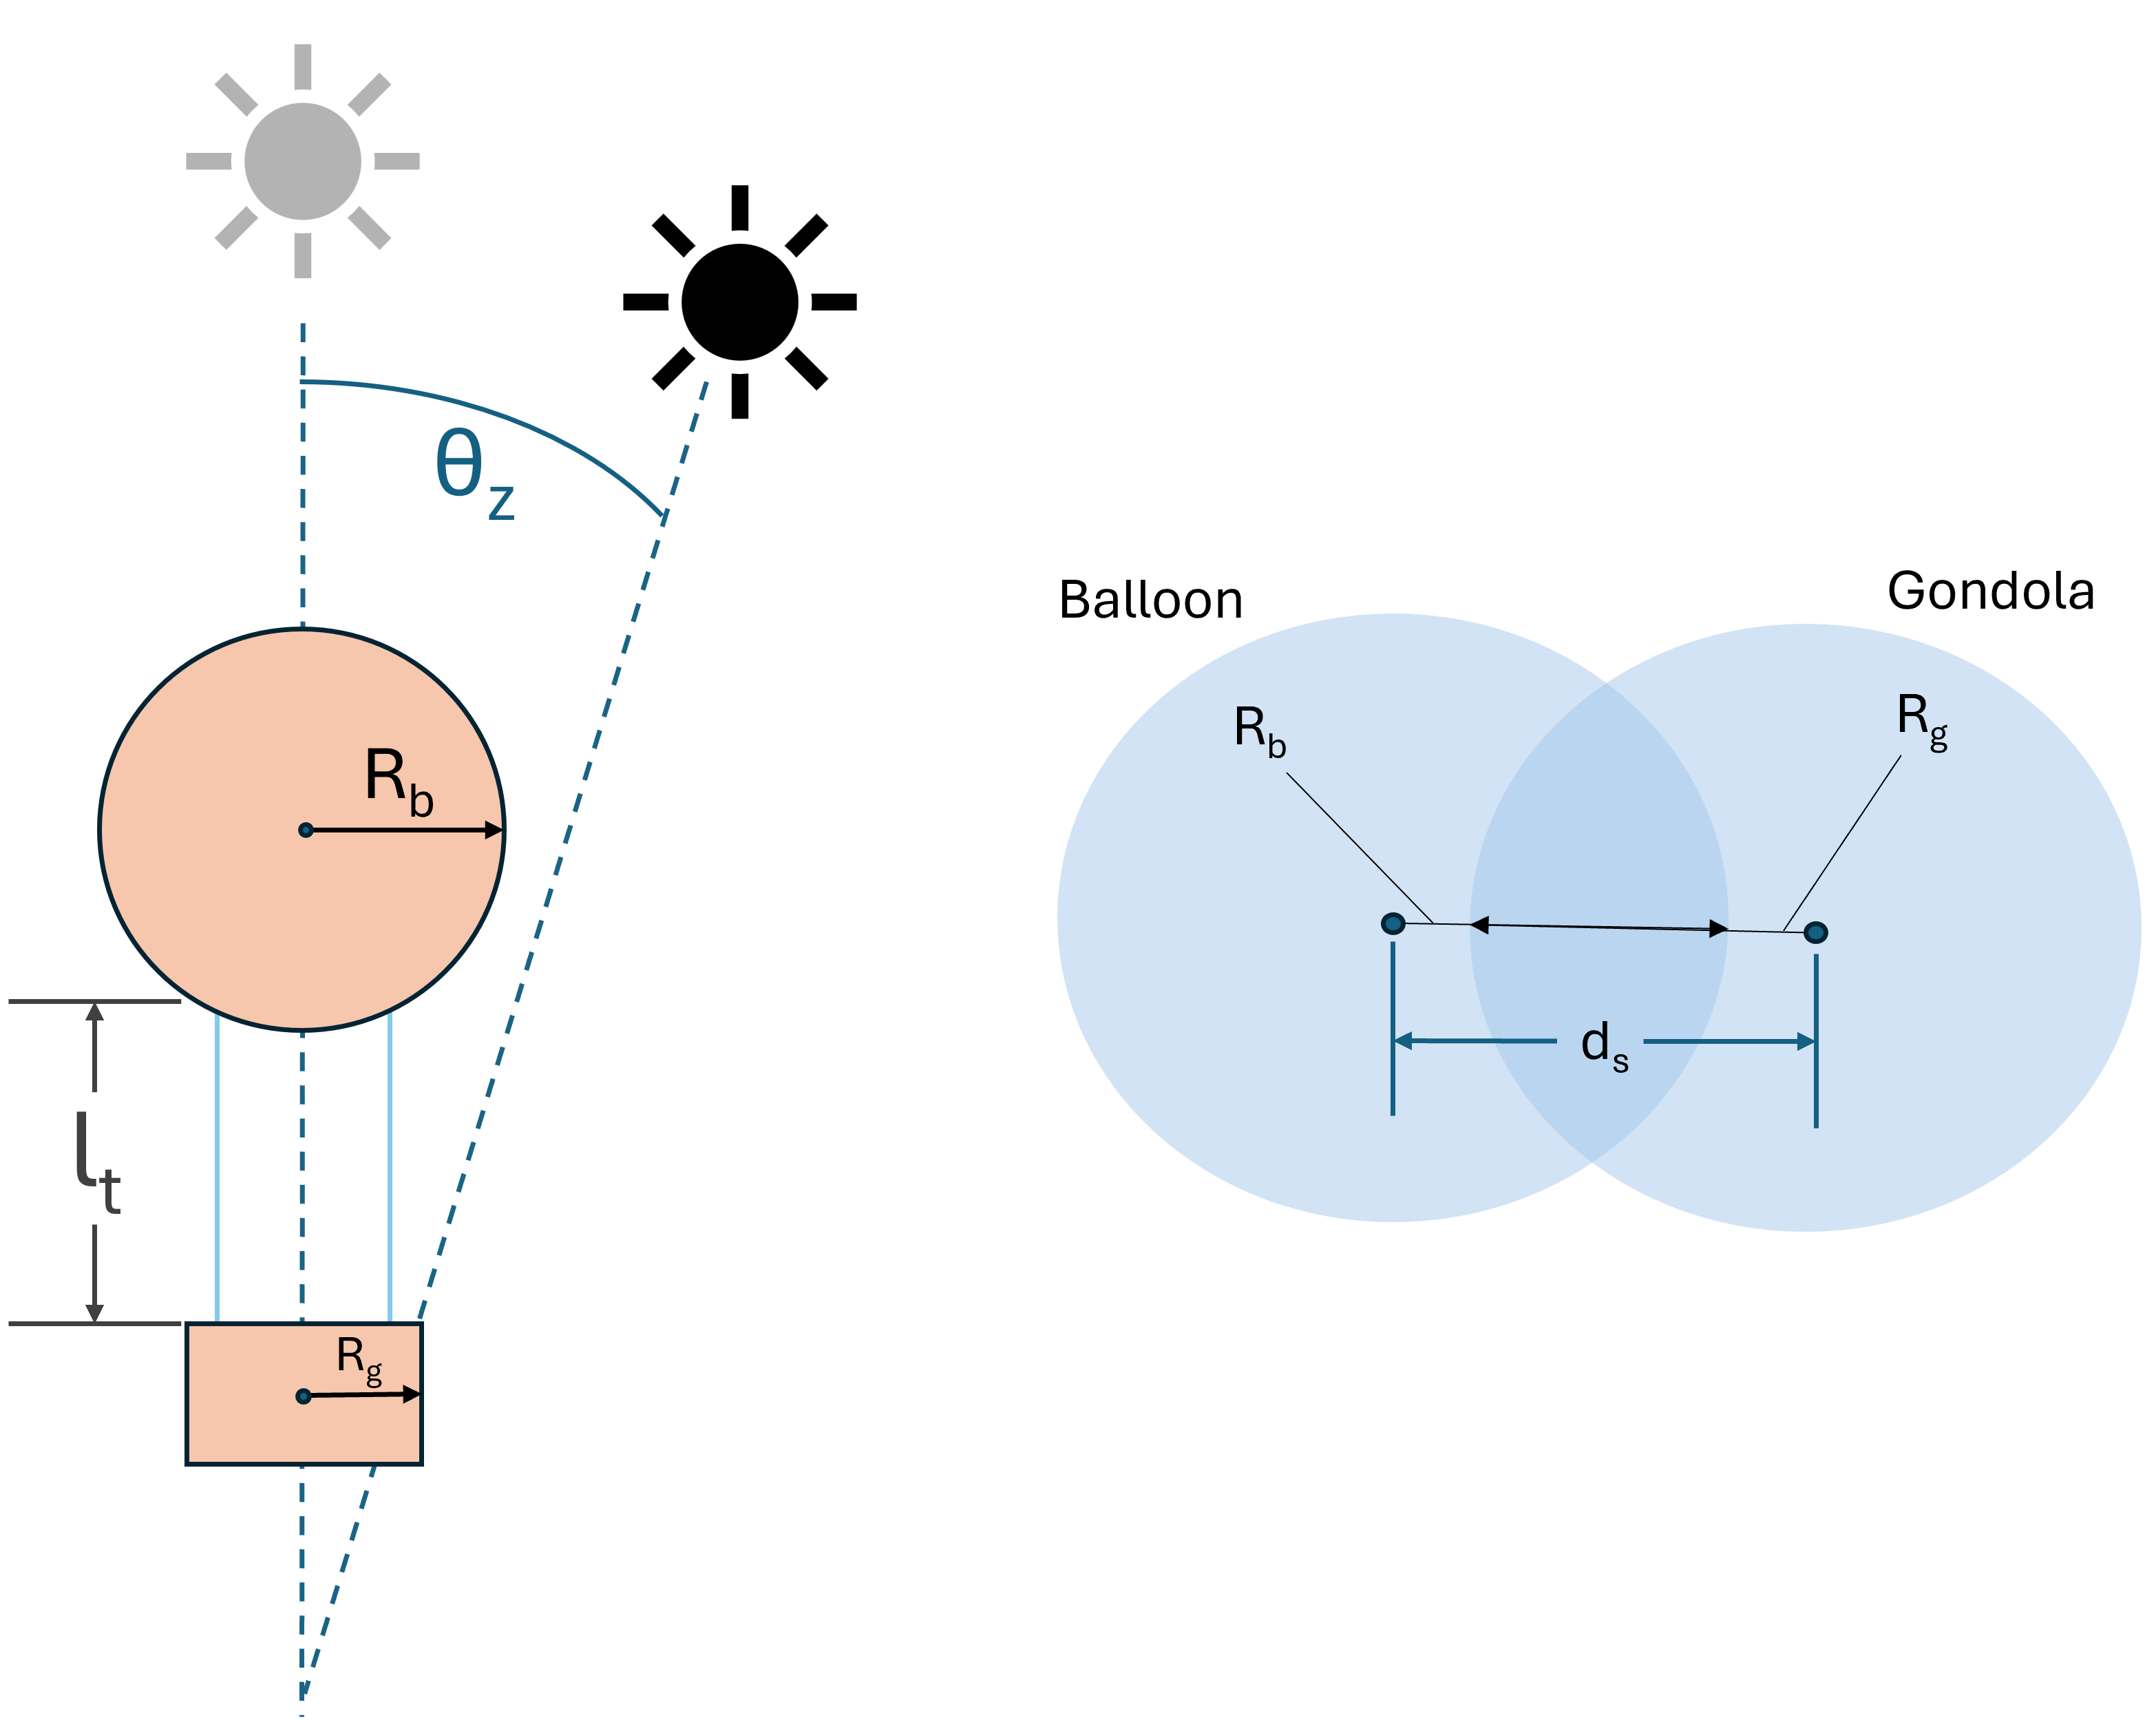
\includegraphics[width=0.44\textwidth]{fig/bitch-ass.png}
    \caption{Enter Caption}
    \label{fig:bitch-ass}
\end{wrapfigure}


Firstly, the solar zenith exit angle, $\theta_{z_{exit}}$ is calculated. For any value of $\theta_{z}$ that is smaller than $\theta_{z_{exit}}$ (closer to the horizon), the gondola is completely out of the balloon's shadow, and this no shadowing effect factor is applied.

When this is not the case, the planar distance between the center of the balloon's projected shadow and the center of the gondola is calculated using:
\begin{equation}
    d_{s}=l\cdot tan(\theta_{z})
\end{equation}
where $d_{s}$ is defined as the shadow center of the gondola plane, and the rest of the variables are defined above. The rest is a geometric ``lens'' problem - a circle-circle intersection (area overlap) which can be calculated using:
\begin{equation}
    A_{i} = \frac{1}{2}\sqrt{(-d_{s}+r+R)(d_{s}+r-R)(d_{s}-r+R)(d_{s}+r+R)}
\end{equation} 

The illumination factor, $f$, is calculated by substracting the overlapping area from the area of the gondola:
\begin{equation}
    f = 1 - \frac{A_{i}}{\pi R_{g}}
\end{equation}

such that the final specific power of the solar arrays can be calculated using
\begin{equation}
    SP=SP_{Landis}\cdot f \cdot k
\end{equation}

where $SP_{Landis}$ is the specific power used from \cite{}, and k is the material coating factor of 5\% which was mentioned earlier.

The final specific power is plotted for 4 different altitudes below in \autoref{fig: sp-altitude}
\begin{figure}[H]
    \centering
    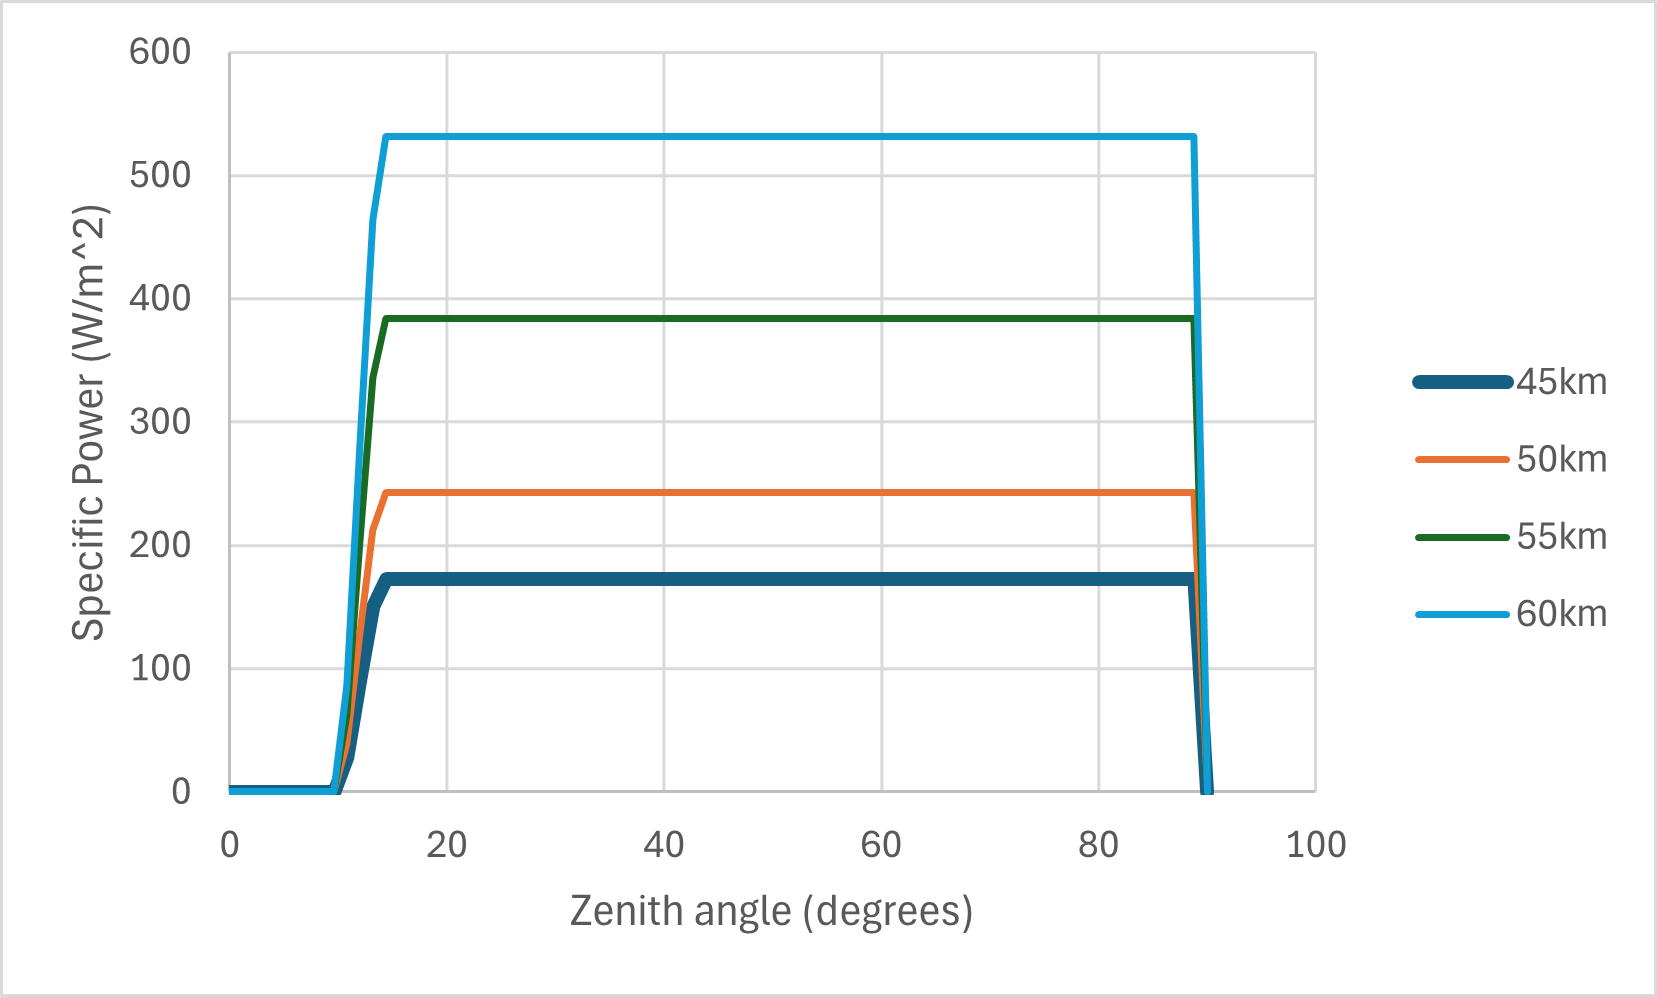
\includegraphics[width=0.75\linewidth]{fig/specific-power-altitude.png}
    \caption{Specific power output of triple junction solar cell over a Venus day for four different realistic flying altitudes.}
    \label{fig: sp-altitude}
\end{figure}

Before calculating the total expected area and mass of the solar array, a degradation factor is applied to find out the power output at EOL.

\begin{equation}
    SP_{EOL} = SP_{BOL} \cdot L_{d}
\end{equation}

where $L_{d}$ is the degradation factor defined sequentially.
\begin{equation}
    L_{d} = (1-l_{d})^{n}
\end{equation}
where $l_{d}$ is the yearly degradation factor, and n is the mission duration in years.

Thus, to achieve the peak power requirement of 190.41 [W] at EOL, the solar arrays must have areas and masses displayed in \autoref{fig: solar-mass-area}

\begin{figure}
    \centering
    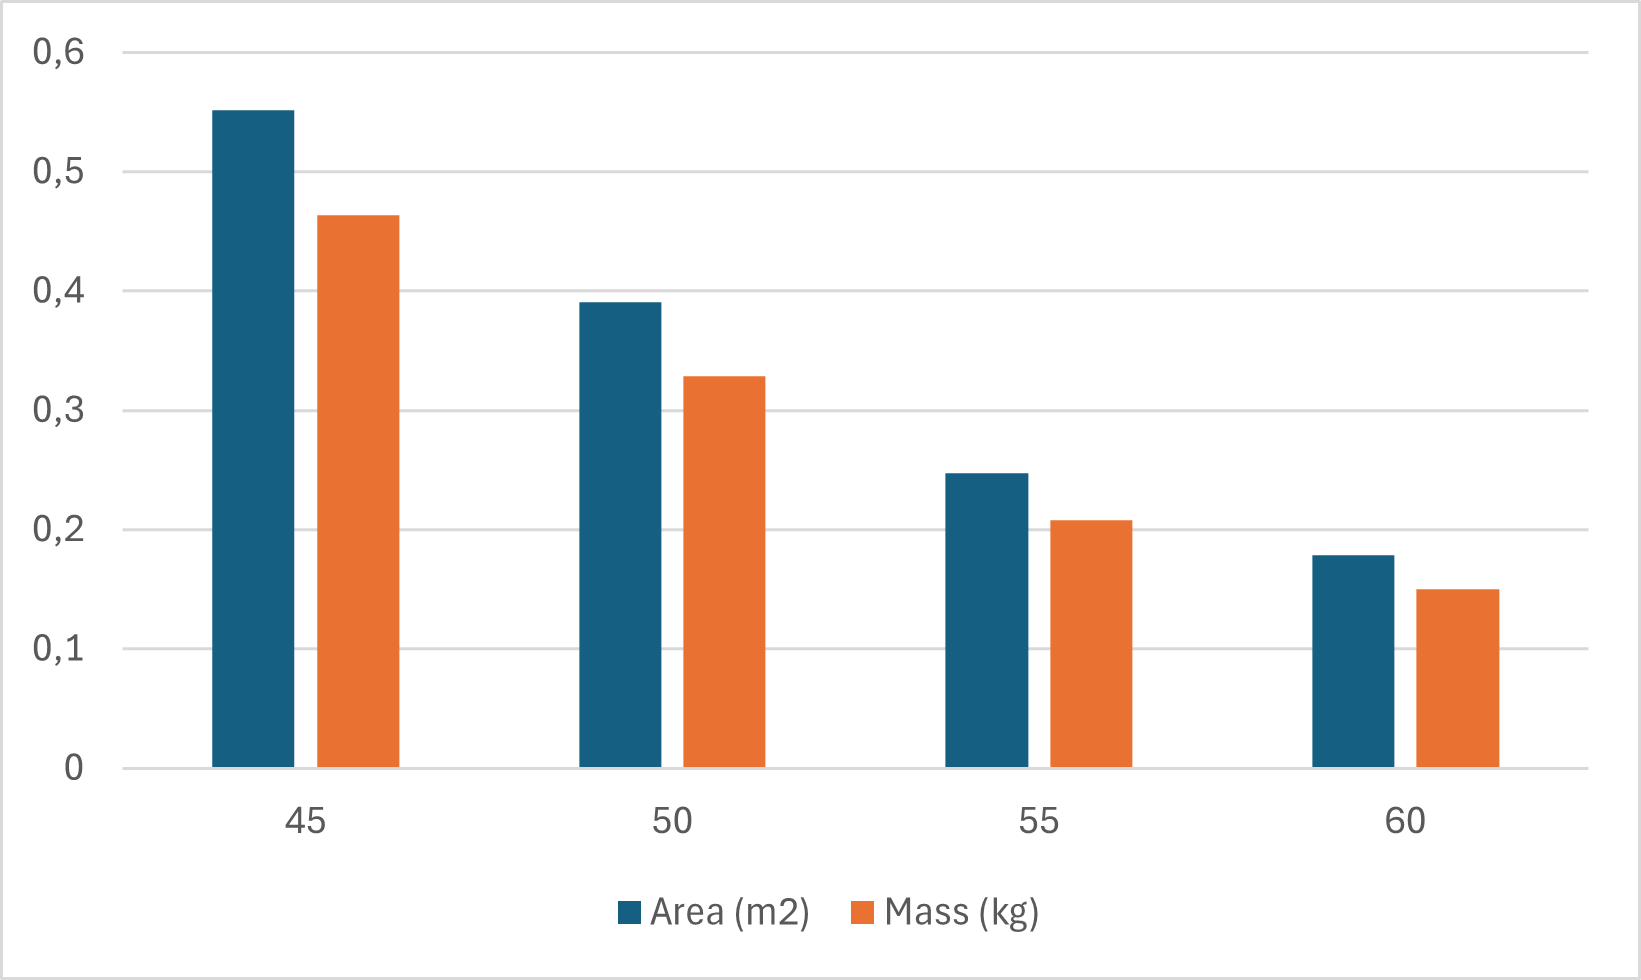
\includegraphics[width=0.75\linewidth]{fig/mass-area-solar.png}
    \caption{The area and mass of the solar array required to generate the required power needed during a Venus day for four different potential flying altitudes.}
    \label{fig: solar-mass-area}
\end{figure}

Note that the sizing of the energy storage unit that will accompany the solar arrays is carried out in \ref{sub:energy-storage}.

\subsubsection{RTG}

Upon consultation with David Jameux (coach), and Colin Wilson (external expert), it was advised to not seriously consider RTGs for the power subsystem of VISTA, as although it would enhance scientific investigation capabilities (especially during the night), this would come at a heavy complexity, and cost penalty. Nevertheless, a preliminary mass sizing is carried out for feasibility's sake. Using NASA's factsheet for the Advanced Stirling Radioisotope Generator (ASRG), the total mass would come out to be  as 48 [kg] for a 195 [W] power output - >3x heavier than the solar + battery option.

\subsubsection{Hybrid}

Not a realistic option for the reasons outlined above, while also the RTG also cannot be scaled down linearly to size it mass and power output appropriately.

\subsection{Energy Storage}
\label{sub:energy-storage}

For the secondary energy storage unit that will power VISTA during night periods, five options were initially considered:

\begin{itemize}
    \item Batteries
    \item Regenerative Fuel Cells (RFCs)
    \item Flywheels
    \item Phase Change Materials
    \item Molecular Solar Thermal (MOST)
\end{itemize}

From these five options, \textbf{phase change materials} and \textbf{MOST} were discarded, because the energy they store can only be released as thermal output and not electrical output without the addition of a complimentary conversion architecture that would significantly increase complexity and mass of the power subsystem. \textbf{Flywheels} were also discarded because they have a very fast discharge cycle (<15 minutes max) which is unsuitable for the supplying power to VISTA during night periods that can last up to 4 days.

Thus, a more detailed analysis was carried out to compare batteries and RFCs.

Using SMAD, the ideal battery capacity is the average night load, $P_{e}$, times the night duration, $T_{e}$. This ideal capacity must be increased to include the battery-to-load transmission efficiency, $n$, and the $DoD$ constraints. Furthermore, the total battery capacity will be split between two batteries to increase the points of failure. Lastly, a degradation factor, $d$, is applied to ensure the battery can deliver the required energy load at EOL. The battery capacity is calculated using 
\begin{equation}
    C_{r} = \frac{P_{e}\cdot T_{e}}{DoD\cdot n \cdot N \cdot d}
\end{equation}

Using values from earlier, $P_{e}=12.45 \hspace{1mm}[W]$ and $T_{e}=4.5\hspace{1mm}[days]$. The number of batteries, $N$, is simply 2 (one actual and one redundant battery). The depth of discharge, $DoD$, is taken as 75\% \footnote{Note that this value might seem a bit low for modern-day batteries that can achieve $DoD$ of >90\%, but 75\% is used to reduce overall battery cycling degradation.}. The transmission efficiency battery-to-load is taken as 90\% from SMAD. Finally, the degradation factor $d$, is taken as 0.8.

Thus, the final battery capacity for a single battery is 
\begin{equation}
    C_{r}= 1185.714 \hspace{1mm} [W-hr]
\end{equation}
and the total battery capacity is $C_{r}=2\cdot 1185.714=2371.428$ [W-hr].

Quoting a specific energy from the LP 33037 60Ah Space Cell (Li-ion battery) from EaglerPitcher Technologies of $160$ [W-hr/kg], then the mass of one battery is $7.411$ [kg] and the total mass of the batteries is $14.822$ [kg]

Regenerative fuel cell (RFC) energy storage was sized using the same methodology as the Li-ion battery, with appropriate parameter substitutions: specific energy of $60$ [Wh/kg] (system level, estimated for the mission's $<5$ [kWh] scale per the trends in NASA Glenn 2022 [NTRS 20220010931]), utilization fraction of $0.90$ (replacing battery DoD), discharge efficiency of $0.55$ (fuel cell electrochemical efficiency), and EOL factor of $0.90$ (consistent with reported RFC stack degradation of 1–2\% per year). The resulting RFC system mass of ~74 [kg] is approximately 5× the LFP baseline of 14.822 [kg]. Although the RFC specific energy targets reported in the literature reach 300–790 [Wh/kg] (Letellier 2011; Mitlitsky 1999), these apply to systems at >10 [kWh] scale where converter masses amortize effectively. At the mission's required energy scale, fixed converter and balance-of-plant masses dominate, yielding a system specific energy substantially below modern Li-ion pack-level values.

Thus, for a solar array + secondary energy storage configuration, a Li-ion battery will be used. Note that this brings the total mass of the power subystem (including solar array) to $15.150$ [kg].

\subsection{Power Conditioning and Distribution Unit}
The consolidated reference architecture for European spacecraft power systems is distribution through Latching Current Limiters (LCLs), which have emerged as the European baseline over several decades of mission heritage.

Modern small spacecraft PCDUs are commodity products (e.g. AAC Clyde Space), so for a preliminary design the baseline parameters from such existing flight heritage units will be used.

\subsubsection{Top-level architecture decisions}

\begin{table}
    \centering
    \small
    \begin{tabular}{|p{2.5cm}|p{5cm}|p{7cm}|}
        \hline
         Parameter  & Choice & Rationale\\
        \hline
        Bus voltage & 28V &European and US space baseline for small-to-medium spacecraft. \\
        Topology &Single regulated main bus with point-of-load conversion.  &Loads each have their own DC-DC converter that takes 28V form the main bus and produces whatever local voltage they need. \\
        Source regulation &Maximum Power Point Tracking (MPPT)  &MPPT regulates the solar array operating point to maximize power extraction under variable insolation. This is mandatory for VISTA given the highly variable Venus cloud illumination. \\
        Distribution and protection &LCL/RLCL  &From ECSS-E-ST-20-20C \\
        \hline
    \end{tabular}
    \caption{Caption}
    \label{tab:placeholder}
\end{table}


\subsubsection{Functional decomposition of the PCDU}

\textbf{Block 1: Solar Array Regulator (MPPT)}




\chapter{ADCS}
\label{chapter:ADCS}

% small intro

% requirements + context -> what we have to do and for what

% DOT and pruning based on constraints + other subsystems

% \begin{itemize}
%     \item intro
%     \item requirements + constraints -> what we have to do -> scope
%     \item ADCS
%     \begin{itemize}
%         \item attitude determination
%         \begin{itemize}
%             \item DOT
%             \item pruning
%             \item one option left -> IMU
%         \end{itemize}

%         \item attitude control
%         \begin{itemize}
%             \item dot
%             \item model
%             \begin{itemize}
%                 \item reasoning to find out what we need and why
%             \end{itemize}
%             \item ref paper etc
%             \item method and assumptions
%             \item sensitivity analysis (inputs vs outputs)
%             \begin{itemize}
%                 \item constraints + dependencies from the other subsystems
%             \end{itemize}
%             \item conclusion -> final baseline
%             \begin{itemize}
%                 \item length
%                 \item n cables
%                 \item attachment radius
%                 \item damping
%                 \item DOT
%                 \item passive actuators
%                 \item final baseline -> what is preferred -> input for structural implementation
%                 \item dynamic insights
%                 \item MMOI
%                 \item symmetry
%                 \item aerodynamic configuration
%                 \item other preferences
%                 \item mass cables
%             \end{itemize}
%         \end{itemize}
%     \end{itemize}

%     \item conclusion
%     \begin{itemize}
%         \item final baseline
%         \item outputs
%         \item inputs for the other subsystems
%         \begin{itemize}
%             \item structures (all the above)
%             \item power (visibility, cable length)
%             \item communications -> processing both payload and imu onboard; also antenna?
%             \item GNC (IMU and absolute attitude)
%             \item ISRU (cable length?)
%             \item payload (radiometer) -> DH
%         \end{itemize}
%     \end{itemize}

% \end{itemize}

The VISTA aerobot is a suspended balloon–gondola system rather than a regular rigid spacecraft, hence its ADCS is not a standard three-axis pointing system. Instead, ADCS focuses on determining and tracking the local dynamic state of the gondola, including attitude, angular rates, oscillations, and post-deployment residual motion. Because no subsystem requires precise pointing, the main objective is to keep the motion bounded, observable, and compatible with the other subsystems. Furthermore, the dynamic behaviour of the gondola has to be assessed to correct the raw scientific measurements obtained by the payload, such as the variations in windspeed. Functions such as global navigation (GNC), altitude control (GNC), measurement numerical correction (C\&DH), deployment control (EDD), and structural verification (STR) remain outside the scope of ADCS. 

This chapter presents the process and rationale for selecting the ADCS configuration, which entails: attitude determination, attitude control/damping, and the dynamic configuration parameters (length of the suspension cables $L_{susp}$, the number of suspension cables $N_{susp}$, the attachment radius $r_{susp}$).

\section{ADCS Constraints, Interfaces and Design Drivers}
\label{sec: ADCS constraints, interfaces and design drivers}

The ADCS design is strongly driven by both the context of the mission and by the constraints imposed by the other subsystems. When it comes to the mission environment, classical attitude references become limited \cite{Cutts2022VenusAerobot}. Star trackers, sun, horizon and surfaces sensing become unreliable due tot the cloud scattering, while magnetic heading cannot be used due to the lack of Venusian magnetic field.

Regarding the subsystem interfaces, the Payload requires accurate attitude metadata for corrected scientific measurements (eg. wind sensor). However, no direct pointing is needed for the proper functioning of instruments. This also applies to the Communications subsystem by choosing omni-directional antennas. The GNC subsystem employs and IMU that can be shared with the ADCS if it is part of the chosen configuration. Furthermore, the Power subsystem requires a minimum cable length of $10$m to mitigate the obstruction of the solar panels, and longer is preferred. 

Moreover, the ADCS and Structures share significant parameters, as the structural configuration has a profound impact on the dynamic behaviour of the aerobot. The shared parameters include: gondola mass, CG position, inertia tensor, geometry, cable length, cable count etc. This complex relationship will be clarified throughout the next two chapters. Lastly, the design must also ensure it complies with the allocated technical budgets for mass, power, cost and data rate. Minimizing these resources is therefore desired. 

\section{Attitude Determination Configuration}
\label{sec: Attitude determination configuration}
\autoref{fig: DOT_ADCS_Attitude} present the design option tree for the Attitude Determination Configuration. Due to the unique mission constraints stated above (eg: cloud scattering, no magnetic field, distance to the Earth), significant pruning has been performed, highlighted in red. This resulted in 4 feasible options left: a 3-axis gyro (IS-1), a 3-axis accelerometer (IS-2), a 6-axis IMU (IS-3= IS-1 + IS-2) and attitude determination based on the Doppler navigation with the orbiter (RS-1). To maximize the attitude knowledge, a combination of the 4 options has been selected as the architecture, highlighted in green. 

The retained baseline is therefore a local inertial sensing approach based on a 6-axis IMU placed close to the gondola centre of gravity for accurate measurement of the intrinsic dynamic motion. Otherwise, additional terms ($\omega \cdot r_{CG-IMU}$) have to be accounted for. The gyroscopes provide angular-rate measurements for swing, yaw, spin, and torsional motion, while the accelerometers provide the 3-axis accelerations, aiding roll and pitch estimations relative to the local gravity and detecting the shocks experienced. As the gyroscope acquires only the relative attitude, which is subjected to IMU drift \cite{Frazier2022}, the orbiter is used to as an absolute reference during the contact times, by leveraging the Doppler technology selected in \autoref{chapter: guidance and navigation} by GNC. Furthermore, as the GNC subsystem also requires a 6-axis IMU architecture, it has been decided that ADCS and GNC will share the exact same low-drift configuration: 3 x Honeywell single axis QA-3000 \cite{HoneywellQA3000} for the accelerations and Safran STIM300 \cite{SafranSTIM300} for the 3-axis gyroscope, as recommended by \cite{Frazier2022}.

\begin{figure}
    \centering
    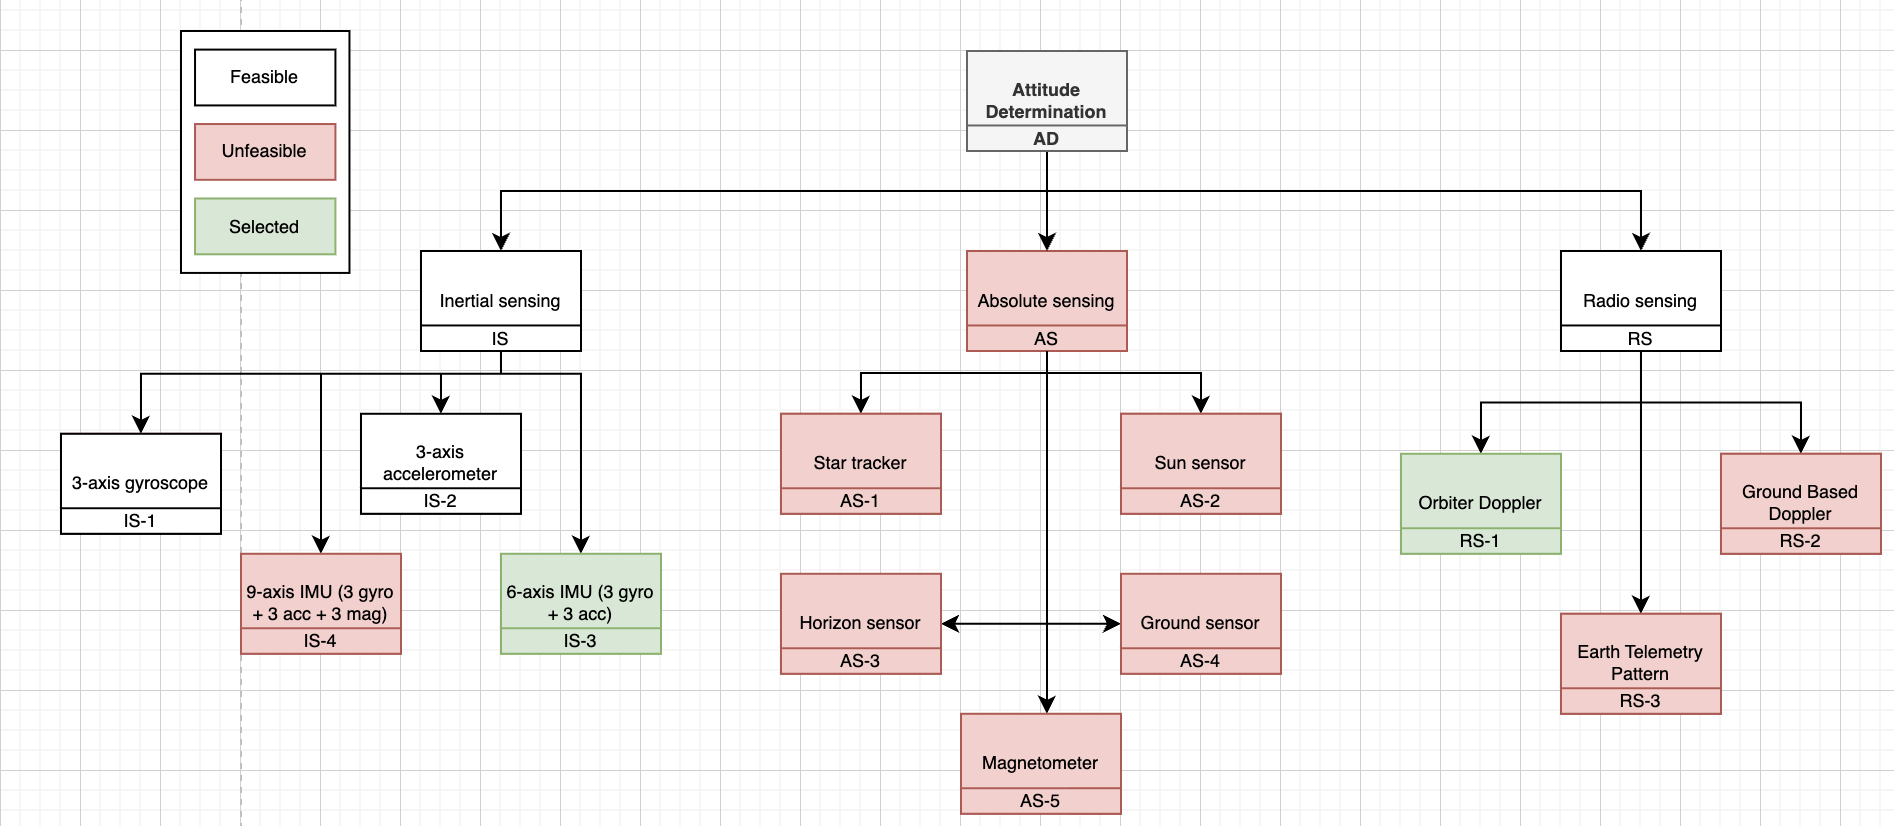
\includegraphics[width=0.9\linewidth]{fig/DOT_ADCS_ATTITUDE.png}
    \caption{Design Option Tree for the Attitude Determination Configuration}
    \label{fig: DOT_ADCS_Attitude}
\end{figure}
%
\section{Dynamic Modeling}
\label{sec: Dynamic Modeling}
The disturbances (aerodynamic gusts, wind shear, vertical winds, internal movements etc.) can excite two main dynamic behaviours throughout the mission: pendulum swing of the gondola beneath the balloon, and torsional oscillation of the gondola around the yaw axis. If the gondola mass distribution is not symmetric, pendulum and torsional motion may also become coupled \cite{Kassarian2021BalloonDynamics}. These behaviours matter because they affect payload measurement quality, structural load (cable tension), IMU range, sampling frequency and others.

\subsection{Methodology}
Informed preliminary design decisions can only be made by getting a better understanding of the complex dynamics of the system. For this, a simplified numerical model, presented in \cite{GithubVenusBalloonProject} has been created, aligned with the methods of Kassarian et al. \cite{Kassarian2021BalloonDynamics}. The suspended balloon-gondola system has been analyzed by dividing the suspension elements in multiple nodes, each with its own degrees of freedom: pendulum angle and torsional angle. Instantaneous snapshots for two different payload configurations are presented in \autoref{fig:gondola_sim}.

\begin{figure}[H]
    \centering

    \begin{subfigure}[b]{0.48\textwidth}
        \centering
        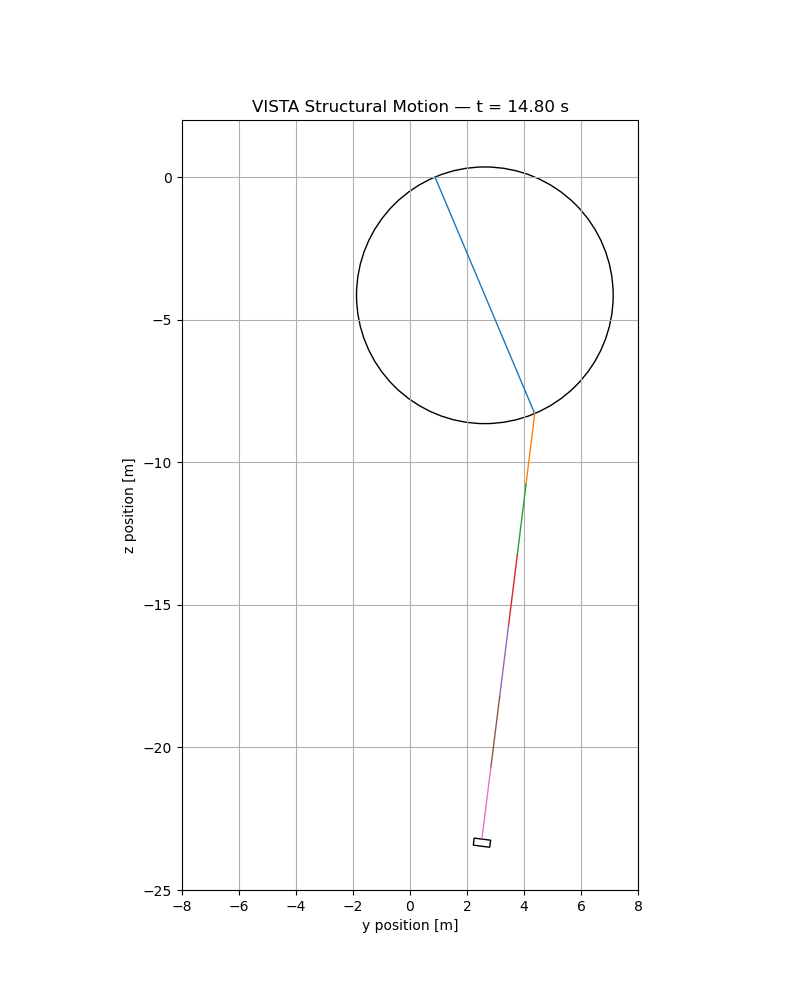
\includegraphics[width=\textwidth]{fig/Gondola_sim.png}
        \caption{Gondola structural simulation}
        \label{fig:gondola_sim}
    \end{subfigure}
    \hfill
    \begin{subfigure}[b]{0.48\textwidth}
        \centering
        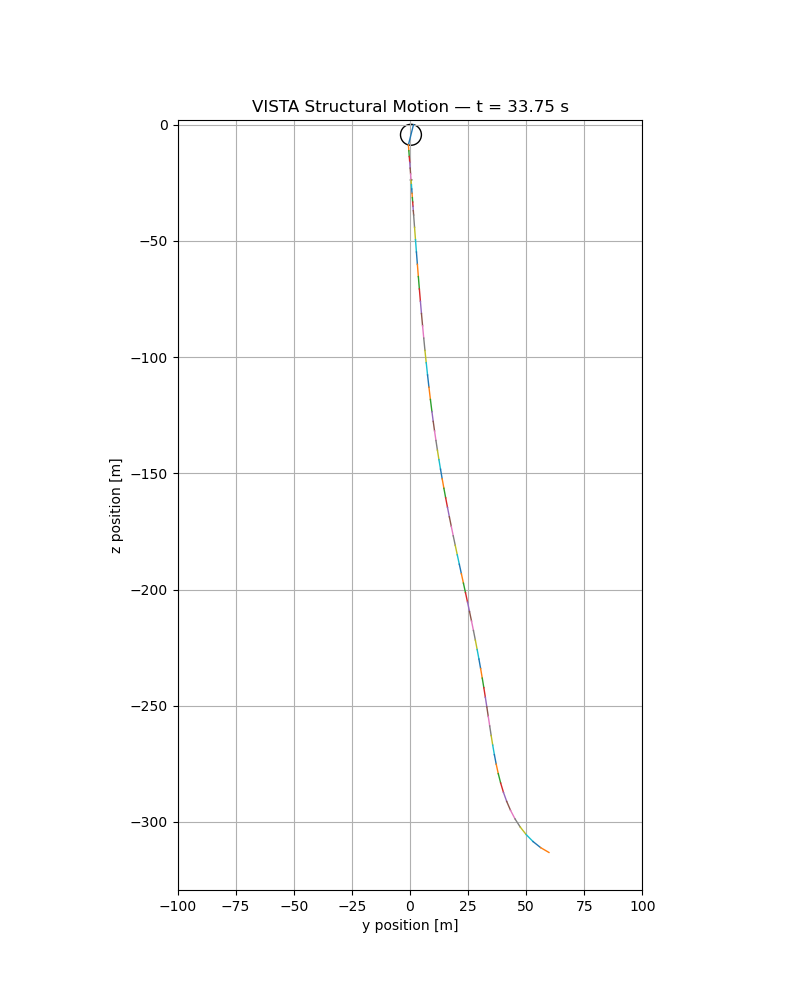
\includegraphics[width=\textwidth]{fig/tether_sim.png}
        \caption{Tether structural simulation}
        \label{fig:tether_sim}
    \end{subfigure}

    \caption{Dynamic simulation results for the gondola and tether configurations}
    \label{fig:struc_sims}
\end{figure}

The governing equations are 
\begin{equation}
    \mathbf{M}_x \ddot{\mathbf{x}} + \mathbf{C}_x \dot{\mathbf{x}} + \mathbf{K}_x \mathbf{x} = \mathbf{F}_x(t) \text{ and }
    \\
    \mathbf{M}_z \ddot{\mathbf{z}} + \mathbf{C}_z \dot{\mathbf{z}} + \mathbf{K}_z \mathbf{z} = \mathbf{T}_z(t)
\end{equation}
where $\mathbf{M}$, $\mathbf{C}$, and $\mathbf{K}$ are the mass, damping, and stiffness matrices for the pendulum/torsional oscillations, and $\mathbf{F}(t)$ represents the simplified disturbance inputs or initial conditions. For a detailed derivation of these equations, the reader is encouraged to delve into \cite{Kassarian2021BalloonDynamics}.

The model takes as inputs the disturbances and the architecture parameters and is used to compute the gondola maximum swing and yaw angles, angular rates, angular accelerations, natural frequencies, dominant periods, settling times, and a the maximum cable tension. It must be noted that the model relies on several assumptions, such small-angle approximations, gondola symmetry and damping modeled directly in the damping coefficients. These aspects will be refined in the further phases of the design.

\subsection{Sensitivity Analysis}
\label{subsec: Sensitivity Analysis}
A sensitivity analysis was performed to assess how the main suspension design parameters influence the dynamic response of the balloon–gondola system. The trends are compiled in \autoref{tab:adcs_sensitivity_trends}, providing valuable insights for the configuration selection from \autoref{sec: configuration selection}.


\begin{table}[htbp]
\centering
\caption{Sensitivity trends for increasing the main suspension design parameters.}
\label{tab:adcs_sensitivity_trends}

\renewcommand{\arraystretch}{1.35}

\begin{tabularx}{0.92\textwidth}{
>{\raggedright\arraybackslash}p{2.6cm}
>{\centering\arraybackslash}X
>{\centering\arraybackslash}X
>{\centering\arraybackslash}X
>{\centering\arraybackslash}X
>{\centering\arraybackslash}X
}
\toprule

\textbf{Input varied} &
\textbf{Period} &
\textbf{Amplitude} &
\textbf{Rate} &
\textbf{Settling time} &
\textbf{Tension} \\

\midrule

$L_{\mathrm{susp}}$
& \textit{I / I}
& \textit{E / I}
& \textit{NM / D}
& \textit{I / I}
& \textit{E / E} \\

$N_{\mathrm{cables}}$
& \textit{E}
& \textit{E}
& \textit{E}
& \textit{E}
& \textit{E} \\

$r_{\mathrm{susp}}$
& \textit{E / D}
& \textit{E / D}
& \textit{E / I}
& \textit{E / D}
& \textit{E} \\

\bottomrule
\end{tabularx}

\vspace{0.3cm}

\begin{minipage}{0.92\textwidth}
\footnotesize
\textit{For combined entries, the first trend refers to the pendulum response and the second to the torsional response.}
Legend: E = equal, I = increase, D = decrease, NM = non-monotonic.
\end{minipage}

\end{table}

The sensitivity results show that suspension length mainly controls the time scale of the suspended system. Increasing $L_{susp}$ increases the dominant pendulum and torsional periods and reduces the yaw-rate response, but it also increases settling time, angular amplitudes, and the physical balloon--gondola separation. The number of cables $N_{susp}$ has little effect on the global pendulum and torsional response, so its relevance is mainly structural: load sharing, redundancy, and deployment complexity. The attachment radius is the dominant torsional design variable. Increasing $r_{susp}$ stiffens the torsional mode and reduces twist amplitude, but it also increases yaw-rate response and torsional interface demand. Moreover, the layout of the gondola has also been analyzed. It was found that, for the same mass, a geometry with a greater mass moment of inertia (MMOI) is desirable, as it makes the design more resistant to disturbances. For these reasons, out of the 3 geometries considered in \autoref{Chap: Structures}, the spherical one has been discarded.

\section{Configuration Selection}
\label{sec: configuration selection}

The aim of this section is to select the simplest feasible configuration that keeps the gondola motion bounded, observable with acceptable uncertainty, and compatible with the subsystem constraints outlined in \autoref{sec: ADCS constraints, interfaces and design drivers}. The main design variables considered are the suspension length, number of suspension cables, attachment radius, gondola shape, and damping concept. The selection logic is to first satisfy hard constraints such as positive cable tension, acceptable swing/yaw amplitudes ($<10 ^\circ$), power-driven clearance ($L_{susp}>10$m), and structural feasibility, and then prefer the lowest-mass and lowest-complexity solution that provides acceptable dynamic behaviour.

For this final point, the main objectives are represented by: minimization of angular amplitudes for accurate modeling and coupling mitigation, minimization of angular rates to IMU uncertainty reduction and achievable sampling rate, minimization of the settling time. However, these objectives can be conflicting, which is illustrated in the next subsections.  

\subsection{Cable Length $L_{susp}$}
\label{subsec: Cable Length}
For the suspension length, the key trade is between slower, more observable motion and increased amplitudes, mass and complexity due to the risk of entanglement. The sensitivity analysis shows that increasing the suspension length increases both the pendulum and torsional periods, while reducing the rate response. This is beneficial for payload correction and IMU observability because the gondola motion becomes slower and easier to track. However, a longer suspension also increases settling time, deployment complexity, and potential feed-system routing implications for the ISRU. Power currently imposes a preliminary balloon–gondola separation range of minimum $10$m due to the solar panel obstruction considerations. Therefore, the selected baseline value is $15$m, balancing the dynamic objectives while also providing more solar exposure, which is crucial for the demanded power subsystem.

\subsection{Number of Cables $N_{susp}$}
\label{subsec: Number of Cables}
For the number of cables, the dynamic sensitivity results show little change in the global pendulum and torsional response when the number of cables is varied. Therefore, cable count is not mainly a dynamic tuning parameter, but a structural and integration trade. Three cables would reduce mass and complexity, but provide less redundancy and a less robust load-sharing arrangement. Six cables would reduce per-cable loads further, but increase mass, deployment complexity, and entanglement risk. The selected baseline of four cables provides a balanced solution: it gives redundancy compared with three cables (required for the 5-year duration of the mission), allows a symmetric attachment pattern and provides load sharing without the complexity and mass of a six-cable layout.

\subsection{Suspension Radius $r_{susp}$}
\label{subsec: Suspension Radius}
For the attachment radius, the trade is dominated by torsional behaviour. The model shows that increasing the attachment radius strongly stiffens the torsional mode, reducing twist amplitude and torsional settling time. This is expected because the torsional stiffness scales approximately with the square of the attachment radius \cite{Kassarian2021BalloonDynamics}. However, a larger radius also increases yaw-rate response, torsional interface demand, and structural integration complexity. The selected baseline is therefore $0.5$ m, because it provides torsional stiffness while keeping the interface compact. If the radius is larger than the gondola dimensions, it requires a small interface structure, which Structures must implement.
  
\subsection{Damping}
\label{subsec: Damping}
As the nominal mission does not require precise active pointing, full three-axis active attitude control is not selected because it would add mass, power demand, complexity, cost, and lifetime risk without a current pointing driver. Instead, the focus shifts on damping, to minimize the impact of the disturbances and improve the accuracy of the dynamic model and IMU. The selected damping concept is a passive hybrid damping architecture, with frictional pendulum damping at the upper suspension interface and torsional eddy-current damping at the gondola-side yaw interface. This separates the two dominant behaviours: pendulum swing is dissipated near the effective pivot, while yaw/twist is dissipated where the suspension connects to the gondola. The concept is fully passive, fluid-free, requires no operational power, and avoids active control unless future analysis show that passive damping is insufficient. The selected passive hybrid architecture raises the modal damping ratio from the bare flight-chain level of $\zeta \approx  10^-3$ \cite{Kassarian2021BalloonDynamics, Aubin2017TorsionalOscillations} to $\zeta \approx 0.05-0.15$ in the swing mode \cite{NASA_LLIS_19101} and $\zeta \geq 0.05$ in the yaw/torsion mode \cite{DiezJimenez2019PassiveEM}, i.e. an order-of-magnitude improvement on both dominant modes.

The architecture is implemented with four Enidine wire-rope isolators (WR/CR-series) \cite{EnidineWRI} at the upper suspension interface  for pendulum damping, and a Oerlikon Space ECD-100  \cite{Hofer2009WireRope} single compact passive eddy-current rotary damper at the gondola-side yaw interface for torsion.

\section{ADCS Baseline Configuration}
\subsection{ADCS Baseline Configuration}
\label{sec:adcs_baseline}

The selected ADCS architecture is summarised in table \autoref{sec:adcs_baseline}: the suspension geometry from the sensitivity analysis (\autoref{subsec: Sensitivity Analysis}). The subsystem is fully passive in nominal float: a  local 6-axis IMU (shared by GNC) near the gondola CG provides attitude determination and dynamic-state monitoring, while pendulum and torsion are dissipated by dedicated passive dampers at the upper suspension and gondola-side interfaces.

\subsection{ADCS Baseline Configuration}
\label{sec:adcs_baseline}

The selected ADCS architecture is summarized in \autoref{tab:adcs_baseline}, combining the suspension geometry locked from the sensitivity analysis (\autoref{subsec: Sensitivity Analysis}) and the hardware inventory selected. The subsystem is fully passive in nominal float: a local, GNC-shared, 6-axis IMU near the gondola CG provides attitude determination and dynamic-state monitoring, while pendulum and torsion are dissipated by dedicated passive dampers at the upper suspension and gondola-side interfaces.

\begin{table}[h]
\centering
\caption{ADCS baseline configuration: suspension geometry and hardware inventory.}
\label{tab:adcs_baseline}
\begin{tabular}{llccc}
\toprule
Category & Item & Qty / Value & Mass & Power \\
\midrule
\multirow{3}{*}{Geometry}
  & Cable length $L_\mathrm{susp}$       & 15 m  & --- & --- \\
  & Number of cables $N_\mathrm{susp}$   & 4     & --- & --- \\
  & Attachment radius $r_\mathrm{susp}$  & 0.5 m & --- & --- \\
\midrule
\multirow{2}{*}{Sensing}
  & Honeywell QA-3000 accelerometer          & 3 & $\sim$0.21 kg & $\sim$2 W   \\
  & Safran STIM300 gyroscope                 & 1 & $\sim$0.06 kg & $\sim$1.5 W \\
\midrule
\multirow{3}{*}{Damping}
  & Enidine WR/CR wire-rope isolator         & 4 & $\sim$0.8 kg  & 0 W \\
  & Oerlikon Space ECD-100-class ECD         & 1 & $\sim$1.5 kg  & 0 W \\
  & Mounting + margin                        & ---& $\sim$0.7 kg & --- \\
\midrule
\textbf{Total} & & & \textbf{$\sim$3.3 kg} & \textbf{$\sim$3.5 W} \\
\bottomrule
\end{tabular}
\end{table}

\section{Verification and Validation Plan}
 
  
\chapter{Structures and Mechanisms}
\label{Chap: Structures}
\todo{definitions}
Now that the suspension length, number of cables, and attachment radius have been determined by the ADCS subsystem, a trade-off analysis for the gondola design can be initiated. In addition to these geometric constraints, subsystem-driven design preferences such as a high moment of inertia about the z-axis ($I_{zz}$), structural symmetry, and other performance drivers are taken into account. In this chapter ... \todo{finish intro}

\section{Requirements}
To ensure integrity of the overall structures design, several requirements are listed. These requirements contain all criteria the structure design must satisfy, and are given in \autoref{tab:struc_req}.

\todo{fill in TBD values}
\todo{ref REQ01 to entry and paper}

\begin{table}[H]
\centering
\caption{Structures requirements}
\label{tab:struc_req}
\begin{tabular}{ll}
\hline
\textbf{Requirement ID} & \textbf{Requirement} \\
\hline
REQ-STR-01 & The structure shall withstand all load cases corresponding to a maximum acceleration of 50 g during re-entry.\\
REQ-STR-02 & The aerobot and all supporting systems shall comply with the dimensional constraints imposed by the entry capsule. \\
REQ-STR-03 & The gondola mass shall not exceed 200 kg. \\
REQ-STR-04 & The structure shall withstand the TBD environmental loads. \\
REQ-STR-05 & The structural layout shall provide mounting provisions for two communication antennas positioned 180$^\circ$ apart. \\
REQ-STR-06 & The structural layout shall provide mounting provisions for two pyrgeometers aligned along a common axis, with one instrument facing upward and the other downward. \\
REQ-STR-07 & The structure shall supply a mechanism to connect the balloon tethers to the gondola. \\
REQ-STR-08 & The structural configuration shall not have any single-point failures. \\

\end{tabular}
\end{table}

\section{Design Option Tree}
For the gondola shape design, three options were considered: a sphere, cylinder and cuboid. An overview is given in \autoref{fig:STRUC_DOT}. From these options, the sphere was deemed as no viable option, according to the higher MMOI objective outlined in \autoref{chapter:ADCS}.

\begin{figure}
    \centering
    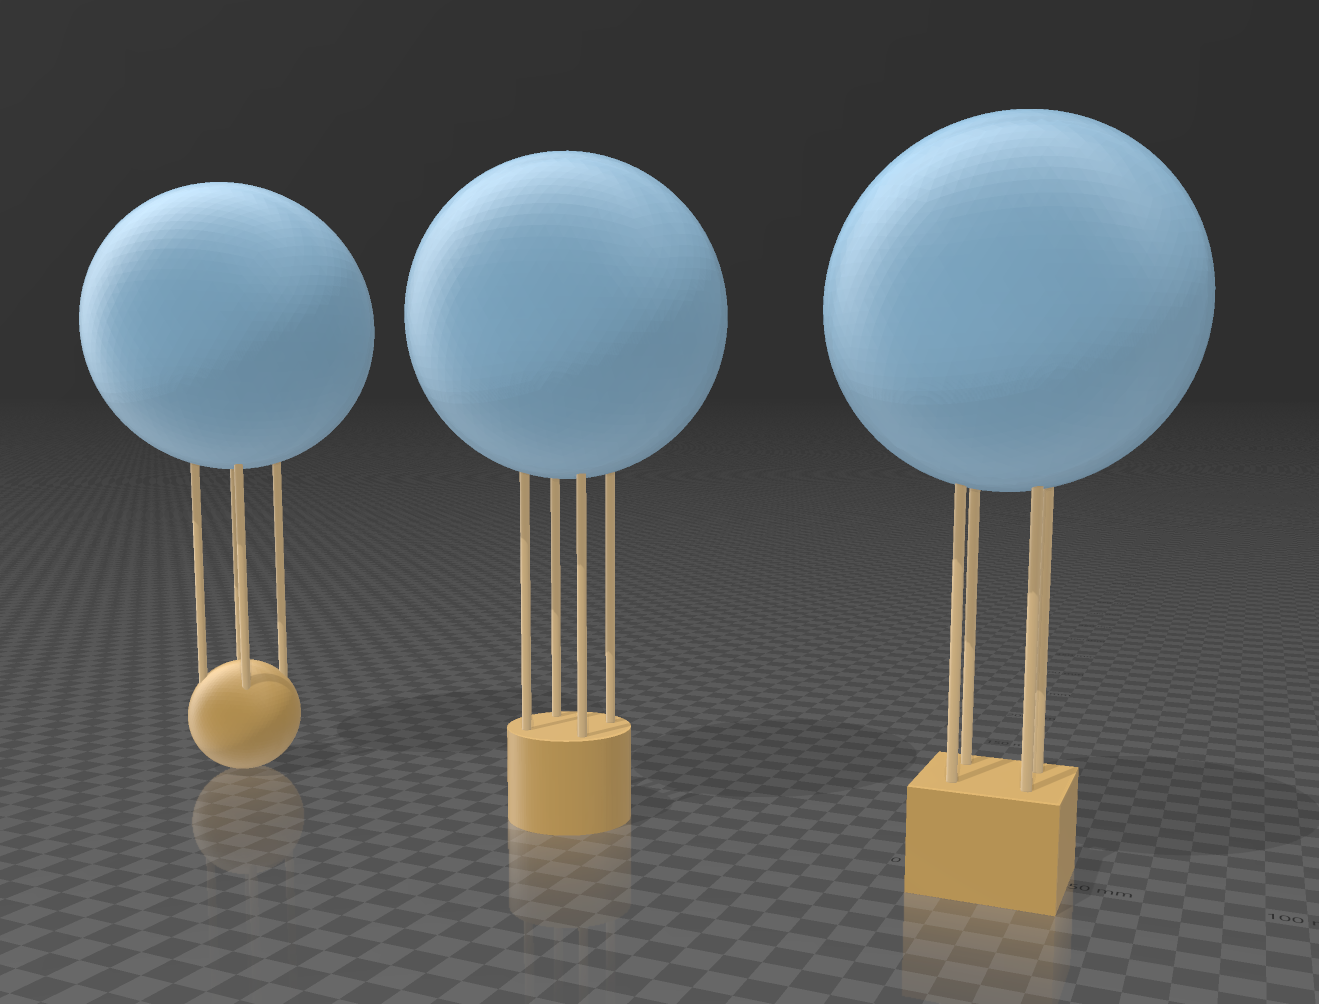
\includegraphics[width=0.5\linewidth]{fig/Gondola_Designs.PNG}
    \caption{The three considered gondola design options, not to scale.}
    \label{fig:STRUC_DOT}
\end{figure}

For the final trade-off for the gondola shape design, further analysis was necessary. For each of the options, their performance was graded upon various parameters. Aside from the requirements from \autoref{tab:struc_req}, additional parameters we considered. These consist of derived performance drivers, e.g. ADCS would benefit from a larger $I_{zz}$. An overview of all relevant drivers is given in \autoref{tab:struc_input1}.

\begin{table}[H]
\centering
\caption{Performance drivers from other subsystems, used as trade-off criteria between gondola shape options}
\label{tab:strc_input1}
\begin{tabular}{ll}
\hline
\textbf{Subsystem} & \textbf{Driver} \\
\hline
General & Minimize volume \\
General & Minimize complexity \\
ADCS & IMU placement close to c.g.\\
ADCS & Maximize MMOI about z-axis; $I_{zz}$\\
ADCS & Preserve symmetry about z-axis\\
Power & Sufficient surface area for solar panel placement $\geq 3900$ cm$^2$\\
Thermal & Minimize surface area\\
\end{tabular}
\end{table}

To begin the analysis, first, all components which needed to be placed inside the gondola were considered as cubes, with sizing based on their estimated volumes. Considering their requirements of orientation, and the parameters given in \autoref{tab:Struc_tradeoffcrit}, all components were laid out in both the cylinder and cuboid options. An overview of these layouts is given in \autoref{fig:struc_layouts}. 
\todo{fire CAD }
\begin{figure}[H]
    \centering

    \begin{subfigure}[b]{0.35\textwidth}
        \centering
        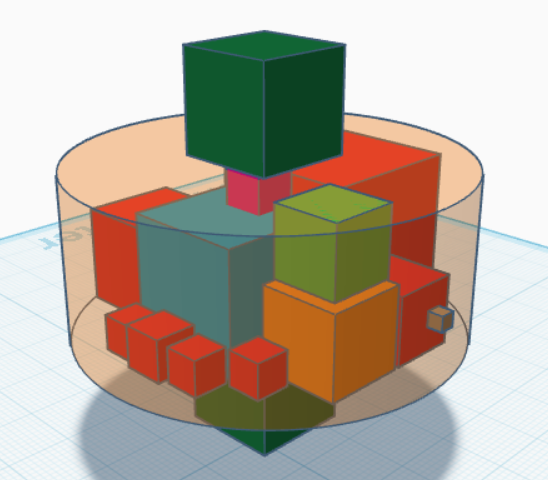
\includegraphics[width=\textwidth]{fig/STRUC_CYL.png}
        \caption{Cylindrical gondola configuration}
        \label{fig:cylinder_layout}
    \end{subfigure}
    \hfill
    \begin{subfigure}[b]{0.35\textwidth}
        \centering
        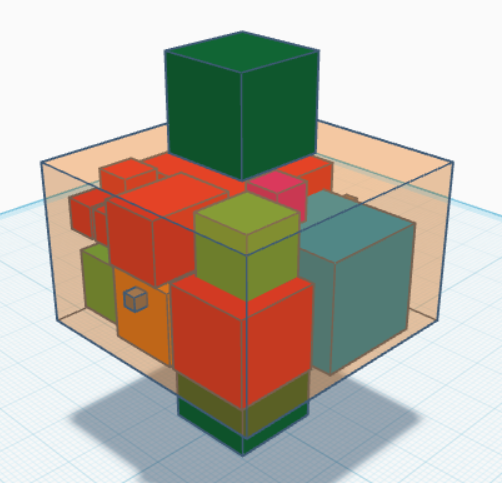
\includegraphics[width=\textwidth]{fig/STRUC_CUB.png}
        \caption{Cuboid gondola configuration}
        \label{fig:cuboid_layout}
    \end{subfigure}

    \caption{Preliminary internal layouts for the considered gondola configurations}
    \label{fig:struc_layouts}
\end{figure}

From these lay-outs, the preliminary estimations of the height, width, surface area and volume were derived for both options, as given in \autoref{tab:struc_est}. From these estimations, it can be seen that the cuboid gondola configuration yields the highest packing density, leading to the lowest surface area and volume. This however, does not directly give the mass and MMOI comparisons, as the thickness of each configurations still needs to be determined. This will be done in \autoref{sub:shell}. 

\subsection{Shell Configuration}\label{sub:shell}
The gondola shell was sized using a preliminary analogy-based sizing approach. The high-level shell design is anchored in comparable small-spacecraft structures that face similar constraints: compact geometry, strict mass limits, high quasi-static launch or entry accelerations. According to \textbf{Rajarajan 2021} and \textbf{Wills 2003} CubeSats and small-spacecraft references must comply with the 50g quasi-static structural load checks, aligned with those estimated in EDD. \textbf{Sekere 2017} CubeSat finite-element study using 2 mm aluminium faces motivates the shell thickness chosen for the VISTA mission. Furthermore, both \textbf{sekere 2017} and NASA SmallSat guidance identify aluminium 6061/7075 as the primary material for shell structures.

The selected baseline is therefore a reinforced gondola rather than a pure thin shell: a 2 mm coated aluminium alloy shell combined with internal ring frames, trays, and reinforced hard points. A simple average-stress check gives approximately $13.5~\mathrm{MPa}$ for the cylindrical shell and $14.2~\mathrm{MPa}$ for the cuboid shell, so global yielding is not the sizing driver. Instead, the 2 mm thickness is justified by local buckling, vibration and coating support. The final preliminary baseline is a cylindrical gondola with $R = 0.29~\mathrm{m}$, $h = 0.25~\mathrm{m}$, $t_{\mathrm{shell}} = 2~\mathrm{mm}$, a aluminium alloy shell/frame, and an estimated shell mass of approximately $5.3~\mathrm{kg}$. The cuboid option, with dimensions $0.43 \times 0.43 \times 0.27~\mathrm{m}$, $t_{\mathrm{shell}} = 2~\mathrm{mm}$, and shell mass of approximately $4.5~\mathrm{kg}$, is retained as a backup in case packaging or mass-budget conflicts emerge. However, the cylinder is preferred due to its symmetry, cleaner inertia properties, lower ADCS coupling risk, larger volume, and structurally efficient curvature.

\subsection{Suspension Cables}
The suspension cable selection was performed as a preliminary trade-off between polymer fibre ropes and metallic cable alternatives, using tensile capacity, mass, cost, environmental robustness and creep/degradation risk as the main criteria.  Three feasible configurations were therefore retained: Vectran/LCP rope with protective jacket/coating, aramid rope with protective jacket, and coated titanium cable. The metallic option is mechanically robust but heavier and still requires environmental protection, while aramid is lightweight but less attractive due to long-term degradation and creep concerns. Vectran/LCP provides the best balance of low mass, high tensile strength, low creep, and existing high-performance rope heritage. The protective layer is assumed to be a fluoropolymer-based coating/jacket, such as PTFE/FEP-type protection, to limit direct exposure of the fibres to sulfuric acid aerosols, UV, thermal cycling, abrasion, and handling damage.

For the current four-cable suspension, each cable is $15 m$ long, giving $60 m$ total cable length. A $4 mm$ Vectran/LCP rope is selected as the preliminary baseline, with an estimated bare rope density of $10g/m$. Hence, the mass of the suspension cables, combined with that of the $300 m$ tether (Payload), the bare rope would weigh $3.6 kg$, and a conservative full cable-package mass of about $5 kg$, including terminations and protection jackets. The expected maximum cable load is approximately $200 N$ per cable, while a conservative safety factor of 10 is applied to account for harsh-environment degradation, creep, coating/jacket damage and other losses. Even with this conservative factor, the design load remains well below the breaking load of a representative $4 mm$ Vectran/LCP rope, which is on the order of $10–15 kN$. Therefore, the cable selection is not strength-limited; the main design drivers are environmental protection, long-duration material stability, termination reliability, and maintaining the protective fluoropolymer coating/jacket throughout the mission. \todo[inline]{\textbf{add references!!!!!}}


    \begin{itemize}
        \item balloon 
        \item hoop stress etc.
        \item skeleton?
    \end{itemize}

\section{Verification Plan}
To verify that the structure will satisfy all given requirements, a verification plan must be established. For each items, an appropriate methods need to be chosen. An overview of these items with corresponding methods is given in \autoref{tab:struc_vnv}.

\begin{table}[H]
\centering
\caption{Verification items and associated verification methods for the structural verification plan}
\label{tab:struc_vnv}
\begin{tabular}{ll}
\hline
\textbf{Item} & \textbf{Verification Method} \\
\hline
Structural mass & Mass properties extracted from CAD model and material property data \\
Geometric constraints & CAD-based envelope compliance assessment against entry capsule interface \\
Load capacity (50 g) & Equivalent static load case analysis supported by analytical calculations \\
Cable safety factor ($SF=10$) & Analytical tension analysis under worst-case loading conditions \\
Hard-point strength & Stress analysis using analytical methods and finite element analysis \\
Global structural stiffness & Simplified analytical model supported by FEM validation \\
Local buckling resistance & Buckling analysis of critical structural elements \\
IMU mounting stiffness & Local stiffness evaluation supported by simplified modal assessment \\
Thermal compatibility & Material and coating selection based on environmental compatibility assessment \\
\hline
\end{tabular}
\end{table}

\section{Mass Budget}
Now that all components have been selected regarding every subsystem, a preliminary mass budget can be made to estimate the total mass. In this analysis, all components were considered, including a margin to account for uncertainties. These margins were based on the maturity, level of confidence and potential design changes of each system. The mass budget overview is given in \autoref{tab:mass_budget}.

\begin{longtable}{llrrrr}
\caption{Cleaned subsystem mass budget} \\
\hline
\textbf{Subsystem} & \textbf{Component} & \textbf{\#} & \textbf{Mass (kg)} & \textbf{Margin} & \textbf{Total mass incl. margin (kg)} \\
\hline
\endfirsthead

\hline
\textbf{Subsystem} & \textbf{Component} & \textbf{\#} & \textbf{Mass (kg)} & \textbf{Margin} & \textbf{Total mass (kg)} \\
\hline
\endhead

ADCS & IMU & 1 & 0.500 & 10\% & 0.550 \\
CDHS & All except computer & 1 & 0.300 & 10\% & 0.330 \\
\hline

ISRU & Valves & 3 & 0.014 & 20\% & 0.051 \\
ISRU & Pump/Intake & 1 & 0.550 & 20\% & 0.660 \\
ISRU & N2 Storage Tank & 1 & 0.180 & 20\% & 0.216 \\
ISRU & Controller Unit & 1 & 0.076 & 20\% & 0.091 \\
ISRU & N2 Separator & 1 & 0.300 & 20\% & 0.360 \\
ISRU & N2 Pump & 1 & 0.250 & 20\% & 0.300 \\
ISRU & Pressure Sensors & 2 & 0.220 & 20\% & 0.528 \\
\hline

PAY & Mass Spectrometer & 1 & 10.900 & 10\% & 11.990 \\
PAY & Nephelometer & 1 & 0.800 & 10\% & 0.880 \\
PAY & Laser Spectrometer & 1 & 0.620 & 10\% & 0.682 \\
PAY & pH Sensor & 1 & 0.350 & 10\% & 0.385 \\
PAY & Weather Instrument Suite & 1 & 0.100 & 10\% & 0.110 \\
PAY & Pyrgeometer & 2 & 1.300 & 10\% & 2.860 \\
PAY & Sonic Anemometer & 1 & 0.400 & 10\% & 0.440 \\
PAY & Optical Particle Counter & 1 & 2.000 & 10\% & 2.200 \\
PAY & Barometer & 5 & 0.050 & 10\% & 0.275 \\
\hline

TCS & Cooling system & 1 & 5.000 & 20\% & 6.000 \\
TCS & Heating system & 1 & 1.000 & 20\% & 1.200 \\
TCS & Temp. sensors & 15 & 0.004 & 20\% & 0.072 \\
\hline

STRUC & Barometer tether & 1 & 4.160 & 40\% & 5.824 \\
STRUC & Tether reel/motor & 1 & 2.000 & 40\% & 2.800 \\
STRUC & Balloon tethers & 4 & 0.200 & 40\% & 1.120 \\
STRUC & Gondola structure & 1 & 5.000 & 40\% & 7.000 \\
\hline

PWR & Solar panels & 1 & 3.000 & 20\% & 3.600 \\
PWR & Battery & 1 & 4.000 & 20\% & 4.800 \\
PWR & PCDU & 1 & 1.500 & 20\% & 1.800 \\
\hline

COM & HRA & 1 & 0.120 & 10\% & 0.132 \\
COM & UHF & 1 & 0.037 & 10\% & 0.041 \\
COM & Other hardware & 1 & 0.080 & 10\% & 0.088 \\
\hline

TTC & X-band transponder & 1 & 3.000 & 10\% & 3.300 \\
TTC & Antenna & 1 & 1.000 & 10\% & 1.100 \\
\hline

\textbf{TOTAL} &  &  & \textbf{49.011} &  & \textbf{61.785} \\
\hline
\end{longtable}

\todo{ref deployment}
Including the margins, the total mass is estimated to be 71.1 kg. It should be noted that this excludes the mass of the deployment stage, as given in \autoref{XX}. In this budget, a significant margin for the structures and mechanism subsystem is given, due to the additional load carrying structures, which are not identified fully yet. 

% TOTAL TABLE (IN CONCLUSION SECTION?)
\begin{table}[H]
\centering
\caption{Parameters derived from gondola lay-out}
\label{tab:struc_est}
\begin{tabular}{lll}
\hline
\textbf{Parameter} & \textbf{Cylinder} & \textbf{Cuboid} \\
\hline
Height (cm) & 25 & 27 \\
Width/Diameter (cm) & 58 & 43 \\
Surface area (cm$^2$) & 9840 & 8342 \\
Volume (cm$^3$) & 66070 & 49923 \\
Thickness (cm) & 0.2 & 0.2 \\
Mass (kg) & 5.3 & 4.5 \\
% Moment of Inertia (kg$\cdot$m$^2$) & & \\
\end{tabular}
\end{table}


\chapter{Deployment}
\label{ch:deployment}
\markboth{Deployment}{Deployment}

The deployment subsystem covers only the entry--descent--deployment--inflation (EDDI) slice: from the entry interface at $\approx 200\,\mathrm{km}$ to a confirmed free-float aerobot state at $\approx 55\,\mathrm{km}$. Long-duration float, altitude control, leakage management, and cruise aerodynamics are therefore interfaces to ISRU/Buoyancy, Navigation, Structures, and CDHS rather than deployment-owned design problems.

The chapter provides the following: driving inputs, option enumeration, trade method, selected architecture, first-order performance characteristics, interfaces, compliance, and residual risks. Architecture tags are defined in Table~\ref{tab:architecture-tag-definitions}; reliability is treated in Section~\ref{sec:deployment-pra}.

\subsection*{Design philosophy}
\label{sec:7-1-1}

Technology maturity is judged using the ECSS/ISO TRL framework, where maturity is assessed relative to the intended product and operating environment~\cite{ECSS_E_HB_11A_2017}. Concepts that are clearly below a Venus-relevant qualification path are therefore not listed one by one in this section: too many branches of the design option tree can be rejected on that basis alone, and repeating that argument would not improve the trade.

The resulting design philosophy is conservative: maximise deployment reliability and avoid spending reliability margin on novelty inside the EDDI chain. Reliability is a key driver because deployment is one-shot; if it fails, the mission is lost before the balloon can perform the science. Since the mission's distinctive value lies in the long-duration Venus aerobot rather than in an exotic entry or deployment system, the deployment architecture should use the most mature, separable, and verifiable solution that can deliver the balloon safely to float.

\section{Deployment scope and driving inputs}
\label{sec:dep-reqs}

\subsection{Entry environment}
\label{sec:7-2-1}

The entry masses used here come from the Baseline Report ROM, but they must be corrected for the selected stored-N$_2$ architecture. In the Baseline Report, the N$_2$ gas was included in the operational float mass but not in the launched entry mass, because that architecture assumed the gas would be generated in situ. For the selected stored-N$_2$ option, this is no longer true: the nitrogen is carried into Venus, so it has to be added back into the entry mass before trajectory, TPS, and parachute sizing are checked.

The entry interface and entry speed are taken from Venus-entry heritage missions. For first-order EDDI sizing, the entry interface is set at $\approx 200\,\mathrm{km}$ and the planet-relative entry speed is taken as $\approx 11\,\mathrm{km\,s^{-1}}$.

\begin{table}[H]
\centering
\caption{Deployment-driving entry-environment inputs.}
\label{tab:entry-env}
\small
\renewcommand{\arraystretch}{1.12}
\begin{tabularx}{\textwidth}{@{}p{0.2\textwidth} p{0.2\textwidth} X@{}}
\toprule
\textbf{Input} & \textbf{Value / basis} & \textbf{Deployment use} \\
\midrule
Entry interface & $\approx 200\,\mathrm{km}$ & Start of the entry--descent--deployment--inflation sequence. \\
Entry speed & $\approx 11\,\mathrm{km\,s^{-1}}$ & Initial condition for aeroshell, TPS, and parachute sizing. \\
Baseline ROM entry masses & 93 / 162 / 393\,kg & Baseline Report entry cases before stored-N$_2$ correction. \\
Stored N$_2$ mass & 107 / 180 / 310\,kg & Baseline Report float-mass cases; the 310\,kg case is also supported by the current 55\,km balloon sizing result of 309.61\,kg. \\
Entry hardware fraction & 0.30 / 0.35 / 0.55 & Baseline Report ROM fraction for aeroshell, parachute, separation, and deployment hardware. \\
Deployment trigger & Mach/$q$ window & Sets the parachute extraction and main-canopy deployment box, following planetary parachute practice where deployment conditions are defined by Mach number and dynamic pressure~\cite{CruzLingard2006}. \\
\bottomrule
\end{tabularx}
\end{table}

\begin{table}[htbp]
\centering
\caption{Baseline-to-stored-N$_2$ entry-mass correction.}
\label{tab:dry-wet-entry-correction}
\scriptsize
\setlength{\tabcolsep}{3pt}
\renewcommand{\arraystretch}{1.15}
\begin{tabularx}{\textwidth}{@{}l
>{\centering\arraybackslash}X
>{\centering\arraybackslash}X
>{\centering\arraybackslash}X
>{\centering\arraybackslash}X
>{\centering\arraybackslash}X
>{\centering\arraybackslash}X@{}}
\toprule
\textbf{Case} &
\makecell{\textbf{Baseline}\\\textbf{entry}\\{[kg]}} &
\makecell{\textbf{Float}\\\textbf{hardware}\\{[kg]}} &
\makecell{\textbf{N$_2$}\\\textbf{gas}\\{[kg]}} &
\makecell{\textbf{Min.}\\\textbf{wet}\\{[kg]}} &
\makecell{\textbf{Entry hw.}\\\textbf{frac.}\\{[-]}} &
\makecell{\textbf{Re-est.}\\\textbf{wet}\\{[kg]}} \\
\midrule
Lower    & 93  & 65  & 107 & 200 & 0.30 & 246  \\
Nominal  & 162 & 105 & 180 & 342 & 0.35 & 438  \\
Bounding & 393 & 177 & 310 & 703 & 0.55 & 1082 \\
\midrule
\multicolumn{7}{@{}p{\textwidth}@{}}{\footnotesize
Minimum wet mass:
$m_{\mathrm{wet,min}} = m_{\mathrm{base}} + m_{\mathrm{N_2}}$.
Re-estimated wet mass:
$m_{\mathrm{wet,re\text{-}est}} =
\dfrac{m_{\mathrm{float}} + m_{\mathrm{N_2}}}{1-f_{\mathrm{entry}}}$,
where $f_{\mathrm{entry}}$ is the Baseline Report ROM fraction assigned to aeroshell, parachute, separation, and deployment hardware.
} \\
\bottomrule
\end{tabularx}
\end{table}

The minimum wet mass only adds the stored N$_2$ to the old Baseline entry mass. The re-estimated wet mass is more conservative because the entry hardware is also scaled around the heavier stored-N$_2$ stack. The bounding case is therefore not closed: it shows that carrying all nitrogen at entry can push the deployment system beyond the original 700\,kg mass cap unless the architecture is resized or descoped.

\subsection{Deployment requirements and active assumptions}
\label{sec:dep-active-assumptions}

The Baseline Report defines the deployment requirements, but leaves several values as TBDs or subsystem interfaces. This section only closes the values needed for the architecture trade. These are screening assumptions, not final trajectory, reliability, or qualification results. The mission-level aerobot survival requirement remains $R>0.90$; deployment reliability is therefore treated as a one-shot design driver to be maximised, not as a separately allocated subsystem requirement at Phase~0.

\begin{table}[H]
\centering
\caption{Baseline deployment requirements and chapter-level assumptions used for the architecture trade.}
\label{tab:deployment-retained-reqs}
\footnotesize
\renewcommand{\arraystretch}{1.12}
\begin{tabularx}{\textwidth}{@{}p{0.15\textwidth} X X@{}}
\toprule
\textbf{Baseline input} & \textbf{Baseline requirement / interface} & \textbf{Closure used in this chapter} \\
\midrule
REQ-F-DEP-01, REQ-C-DEP-02 & Deployment must be compatible with the relay-orbiter geometry and reach the operational float altitude. & Hand-off is set to $\approx55\,\mathrm{km}$, near the lower float band, to limit the initial stored-N$_2$ requirement. \\
REQ-F-DEP-03, REQ-F-DEP-12 & Envelope and gondola must deploy without tearing, snagging, entanglement, or post-inflation damage. & Used as the sequence and clearance driver; recontact, tendon entanglement, and gondola-release risks are penalised. \\
REQ-C-DEP-06, REQ-C-SUB-03 & Stored gas must not be released before the required altitude, and the inflation system must remain within its mass allocation. & Stored N$_2$ is included in the wet entry case; premature release, tankage, and inflation mass remain residual risks. \\
REQ-C-DEP-07, REQ-F-DEP-08, REQ-F-DEP-10 & The EDDI chain must survive entry loads, remain dynamically stable, and decelerate to a deployable state. & A $200\,g_0$ load cap and Mach/$q$ parachute trigger box are used as first-order screening limits, based on Venus ballistic-entry studies using $200\,g$ as a science-payload mechanical limit~\cite{Prabhu2013VenusEntry}. \\
REQ-F-DEP-09, REQ-C-SUB-04 & The stack must fit the entry capsule, while aeroshell and parachute mass remain within the Baseline allocation. & Used as the main packaging and EDL-mass closure. \\
REQ-F-DEP-11, REQ-F-DEP-13--15 & Heat-shield orientation, jettison, structural survival, and thermal survival must close during Venus entry. & Treated as aeroshell and separation constraints; avoidable jettison or recontact risks are penalised. \\
REQ-F-DEP-04 & Successful deployment must be confirmed after release and inflation. & Requires CDHS-coupled deployment-status confirmation after free-float hand-off. \\
REQ-C-MIS-02, REQ-C-MIS-03 & Total aerobot mass is limited to $700\,\mathrm{kg}$ and each aerobot must exceed $90\%$ mission survival probability. & Applies the dry/wet mass correction; deployment reliability is maximised, but no fixed subsystem allocation is claimed. \\
REQ-F-LAU-04--06 & Deployment must not activate before Venus entry, launch locks must release after arrival, and interfaces must be verified before launch. & Folded into release logic and AIT rather than traded as separate architecture drivers. \\
\bottomrule
\end{tabularx}
\end{table}

Altitude control, envelope sizing, leakage management, cruise aerodynamics, and long-duration material ageing remain subsystem interfaces unless they affect initial fill, separation, or free-float hand-off.

\clearpage

\begin{landscape}
\thispagestyle{plain}

\section{Design option tree}
\label{sec:7-3}

The DOT in Figure~\ref{fig:DOTD} defines the deployment-side option space. The selection argument is made in Section~\ref{sec:dep-integration}, where low-maturity and weak-reliability combinations are removed.

\vspace{0.5em}

\begin{figure}[H]
    \centering
    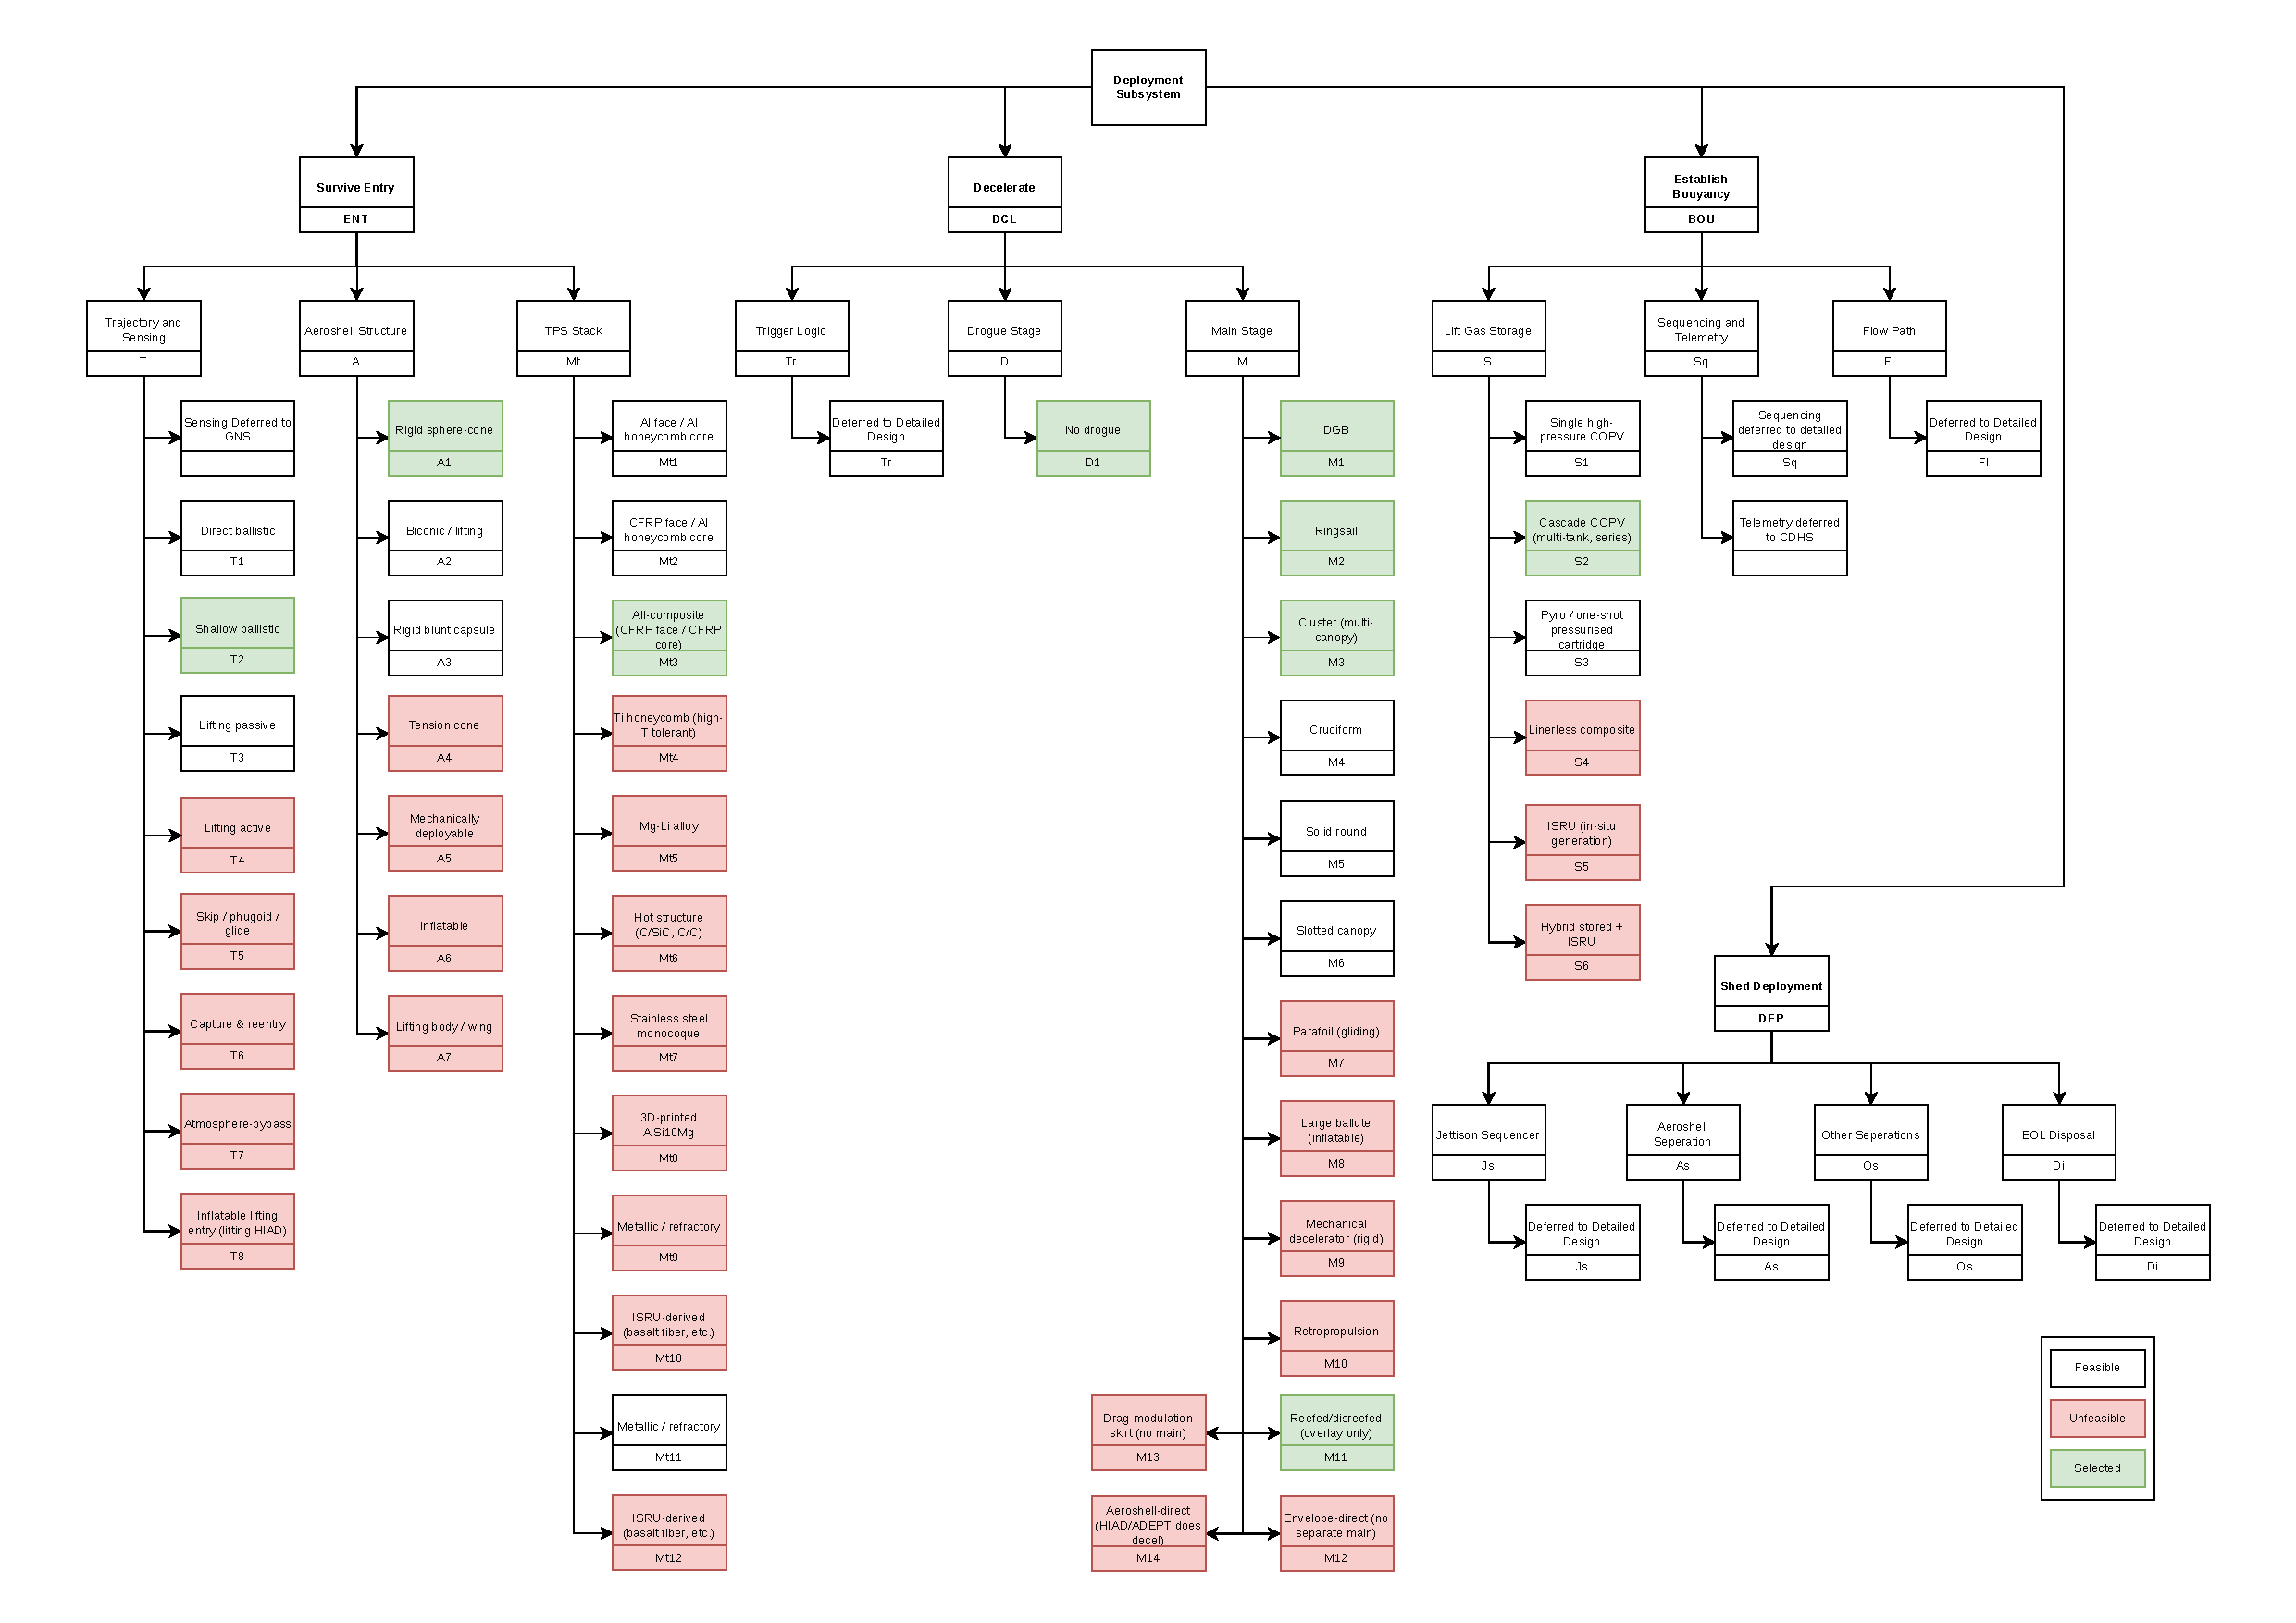
\includegraphics[
        width=\linewidth,
        height=0.8\textheight,
        keepaspectratio
    ]{fig/DOT_Dep.pdf}
    \caption{Design Option Tree for the deployment subsystem.}
    \label{fig:DOTD}
\end{figure}

\end{landscape}

\clearpage


\section{Trade method and architecture selection}
\label{sec:dep-method}

The trade is split into two tracks. Track~1 selects the best independent DOT options, giving the audit tuple $(T^{*},A^{*},M_t^{*},S^{*},M^{*})=(T2,A1,Mt3,S2,M2)$. Track~2 then reopens the architecture space and selects the most reliable feasible deployment architecture. The material axis $M_t$ is not included in the main Cartesian search because material choice is resolved in a parallel trade. Technology maturity is used as a hard filter: Only architectures with TRL~$\geq 7$ today and a credible path to TRL~9 by PDR are retained. This keeps deployment low-risk, reserving the technology risk budget for the novel balloon and long-duration float system. This keeps the lower-maturity risk budget on the floating subsystem rather than the one-shot EDDI chain.

The resulting cascade is summarised in Table~\ref{tab:track2-filter-cascade}. The final selection is $\varepsilon_{\mathrm{RX}}$--Mt3, which maximises reliability while remaining within the entry-mass cap.

\begin{table}[H]
\centering
\footnotesize
\caption{Deployment architecture down-selection cascade.}
\label{tab:track2-filter-cascade}
\renewcommand{\arraystretch}{1}
\setlength{\tabcolsep}{6pt}

\begin{tabularx}{\textwidth}{
@{}
>{\raggedright\arraybackslash}p{0.28\textwidth}
>{\centering\arraybackslash}p{0.08\textwidth}
X
@{}
}
\toprule
\textbf{Stage} & \textbf{Cases} & \textbf{Outcome} \\
\midrule

Raw DOT space
& 4032
& Full $(T,A,S,M)$ architecture space; $M_t$ handled separately. \\

Compatibility filters
& $\approx 120$
& Physically or interface-incoherent combinations removed. \\

TRL filter
& 26
& Only architectures with TRL~$\geq 7$ today and credible path to TRL~9 retained. \\

Class-champion sweep
& 5
& Only $\alpha$, $\varepsilon$, $M_t$, and $T$ families retain feasible contenders. \\

Final selection
& 1
& $\varepsilon_{\mathrm{RX}}$--Mt3 selected: $R=0.992$ with 95\,\% CI $[0.985,0.996]$, $500\,\mathrm{kg}$ ROM entry mass, within the $700\,\mathrm{kg}$ cap. \\

\bottomrule
\end{tabularx}
\end{table}

\subsection{Track 1: independent solution}
\label{sec:track1-independent}
\label{sec:7-3-1}
\label{sec:7-3-3}
\label{sec:dep-d12b}
\label{sec:7-3-2}
\label{sec:dep-d44}
\label{sec:dep-d31}

Each deployment axis is first scored on its own. Detailed archived-branch explanations are removed from the MTR chapter; the key selection logic is retained in Table~\ref{tab:track1-setup}.

\begin{table}[ht]
\centering
\renewcommand{\arraystretch}{1}
\small
\caption{Selected Track~1 independent deployment setup.}
\label{tab:track1-setup}
\label{tab:lift-payoff-screen}
\label{tab:d11-trajectory-screening}
\label{tab:d13-structure-screening}
\label{tab:d12-material-screening}
\label{tab:main-deploy-trigger}
\label{tab:d23-descent-screening}
\label{tab:d31-storage-screening}
\setlength{\tabcolsep}{5pt}
\begin{tabularx}{\textwidth}{@{}p{0.18\textwidth} p{0.18\textwidth} p{0.18\textwidth} X@{}}
\toprule
\textbf{Axis} & \textbf{Selected option} & \textbf{Fallback} & \textbf{Reason} \\
\midrule
Trajectory class & T2 shallow ballistic & T1 steep ballistic & Uses Venus heritage and keeps peak load low without adding lift hardware. \\
Aeroshell architecture & A1 rigid sphere-cone & A3 blunt capsule & Best blunt-body heritage path for a non-lifting trajectory~\cite{Seiff1991,Garvin2022,Steltzner2014}. \\
Aeroshell material & Mt3 all-composite face/core & Mt2 CFRP/Al core & Best mass/interface trade, but coupon qualification remains DEP-2. \\
Lift-gas storage & S2 cascaded COPVs & S3 cartridge & Avoids single-point inflation failure and supports cross-strapped inflation strings. \\
Main descent system & M2 DGB + reefed ringsail cluster & M1 single DGB & Uses DGB heritage with a calmer terminal hand-off~\cite{Knacke1992,CruzLingard2006,Witkowski2013}. \\
\midrule
\multicolumn{4}{@{}l@{}}{\textbf{Track~1 tuple:} $(T^*,A^*,Mt^*,S^*,M^*)=(T2,A1,Mt3,S2,M2)$.} \\
\bottomrule
\end{tabularx}
\end{table}

The main rejected branches are not design drivers. Lifting trajectories add CG-offset, asymmetric TPS, RCS, or GN\&C mass for little benefit because VISTA deploys to a cloud-layer float state rather than a surface landing target. Deployable/inflatable aeroshells and lifting HIAD options remain below the Venus-relevant maturity needed for a one-shot deployment claim~\cite{Mankins1995,Grinspoon2010,Sagdeev1986}. Mt2 stays as the fallback if the Mt3 coupon programme fails.

\subsection{Track 2: integrated architecture ranking}

Track~2 checks whether separate DOT choices can be combined without creating a hidden interface or reliability penalty. The integration vectors are only an internal trade notation.

\begin{table}[H]
    \centering
    \renewcommand{\arraystretch}{1}
    \footnotesize
    \caption{Integration vector taxonomy for the deployment trade space.}
    \label{tab:integration_vectors}
    \begin{tabularx}{\linewidth}{p{0.10\linewidth} p{0.20\linewidth} X p{0.25\linewidth}}
        \toprule
        \textbf{Vector} & \textbf{Axes collapsed} & \textbf{Mechanism} & \textbf{Status} \\
        \midrule
        $\alpha$ & None & Heritage layout; all axes remain separate. & Reference backbone \\
        $\beta$ & A + M & Aeroshell also works as decelerator. & Archived; low TRL \\
        $\gamma$ & S + M & Stored gas inflates a ballute, then feeds envelope. & Archived; reliability too low \\
        $\delta$ & M + envelope & Envelope replaces main decelerator. & Archived; Buoyancy-owned \\
        $\varepsilon$ & S + A & Storage and aeroshell structure share load paths. & Selected in $\varepsilon_{\mathrm{RX}}$-Mt3 \\
        $\zeta$ & A + M + envelope & One inflatable handles entry, deceleration, and float. & Archived; TRL~1 \\
        $\eta$ & T + A & Lifting trajectory needs a lifting aeroshell. & Alternate; reliability too low \\
        $\theta$ & S + M + envelope & One gas reserve supports ballute and envelope. & Archived; CCF dominated \\
        $\iota$ & S + A + M & Storage, aeroshell, and descent tied into one load path. & Archived; insufficient mass/$R$ data \\
        \bottomrule
    \end{tabularx}
\end{table}

\begin{table}[H]
\centering
\small
\renewcommand{\arraystretch}{1}
\caption{Architecture tags used in the deployment ranking.}
\label{tab:architecture-tag-definitions}
\begin{tabularx}{\textwidth}{@{}p{0.22\textwidth} p{0.24\textwidth} X@{}}
\toprule
\textbf{Tag} & \textbf{Role} & \textbf{Definition} \\
\midrule
Track~1 tuple & Independent optimum & $(T2,A1,Mt3,S2,M2)$ selected axis-by-axis without integration credit. \\
$\alpha_1$ & Heritage reference & Single-string uncoupled reference using the T2/A1 backbone, Mt2 fallback material, S1 single COPV, and M1 single DGB. \\
$\alpha_{\mathrm{R3}}$-Mt3 & Redundancy rung & $\alpha_1$ with Mt3 and three-way redundant/cross-strappable P8 inflation strings. \\
$\alpha_{\mathrm{R6}}$-Mt3 & Redundancy rung & Mt3 case with six-way critical-string redundancy; common-cause failure dominates. \\
$\varepsilon_{\mathrm{RX}}$-Mt3 & Selected architecture & T2/A1/Mt3/S2/M2 with $\varepsilon_1$ S+A coupling, functional diversity, and supplier separation. \\
\bottomrule
\end{tabularx}
\end{table}

Figure~\ref{fig:track2_mass_reliability} shows the final ranking. The lightest options were checked, but their reliability is limited by single-string or common-cause failure modes. Among architectures with complete DSE-level mass and reliability estimates, $\varepsilon_{\mathrm{RX}}$-Mt3 gives the highest achievable deployment reliability while remaining within the entry-mass and packaging constraints.

\begin{figure}[H]
\centering
\begin{tikzpicture}[
  label/.style={font=\scriptsize, inner sep=1pt},
  famlabel/.style={font=\scriptsize\itshape, inner sep=1pt},
  keylabel/.style={font=\scriptsize\bfseries, inner sep=1pt},
]
\begin{axis}[
  width=0.95\linewidth,
  height=0.62\linewidth,
  xlabel={$\Delta$ mass vs.\ $\alpha_1$ reference (kg)},
  ylabel={Deployment-subsystem reliability $R$},
  xmin=-55, xmax=45,
  ymin=0.78, ymax=1.01,
  xtick={-50,-40,-30,-20,-10,0,10,20,30,40},
  ytick={0.80,0.85,0.90,0.93,0.95,0.97,1.00},
  yticklabel style={/pgf/number format/.cd, fixed, precision=2},
  grid=major,
  grid style={dashed, black!12},
  axis line style={black!70},
  tick style={black!70},
  enlargelimits=false,
  clip=true,
  scatter/use mapped color={draw=mapped color, fill=mapped color},
  point meta min=7,
  point meta max=9,
  colorbar,
  colorbar style={
    title={TRL},
    ylabel={},
    ytick={7,8,9},
    height=0.55\linewidth,
  },
]
% --- alpha_1 baseline reference line ---
\addplot [draw=black!35, thin, dotted, domain=-55:45] {0.93};

% =========================================================
% FAMILY CLUSTER BACKDROPS (behind markers)
% =========================================================
\draw[fill=blue!10,    draw=blue!55,    thick, rounded corners=6pt]
  (axis cs:-11,0.900) rectangle (axis cs:7,0.945);
\draw[fill=green!10,   draw=green!55,   thick, rounded corners=6pt]
  (axis cs:-28,0.893) rectangle (axis cs:-16,0.924);
\draw[fill=orange!12,  draw=orange!60,  thick, rounded corners=6pt]
  (axis cs:10,0.913) rectangle (axis cs:23,0.953);
\draw[fill=purple!10,  draw=purple!55,  thick, rounded corners=6pt]
  (axis cs:-14,0.865) rectangle (axis cs:-2,0.895);
\draw[fill=gray!15,    draw=gray!60,    thick, rounded corners=6pt]
  (axis cs:-37,0.836) rectangle (axis cs:-28,0.862);
\draw[fill=brown!10,   draw=brown!55,   thick, rounded corners=6pt]
  (axis cs:-49,0.802) rectangle (axis cs:-30,0.834);

% Family tags (compact symbols, INSIDE each box, top-left corner)
\node[famlabel, blue!60!black,   anchor=north west] at (axis cs:-10.7,0.944)  {$\alpha$};
\node[famlabel, green!50!black,  anchor=north west] at (axis cs:-27.7,0.923)  {$\varepsilon$};
\node[famlabel, orange!60!black, anchor=north west] at (axis cs:10.3,0.952)   {$M_t$};
\node[famlabel, purple!60!black, anchor=north west] at (axis cs:-13.7,0.894)  {$T$};
\node[famlabel, gray!50!black,   anchor=north west] at (axis cs:-36.7,0.861)  {$\beta$};
\node[famlabel, brown!60!black,  anchor=north west] at (axis cs:-48.7,0.833)  {$\gamma,\delta,\eta,\theta$};

% =========================================================
% DATA POINTS (26 = 21 single-stack + 5 composites)
% =========================================================
\addplot[
  scatter,
  only marks,
  mark=*,
  scatter src=explicit,
  visualization depends on={\thisrow{size} \as \markersize},
  mark options={scale=\markersize},
]
table[
  x=dm,
  y=R,
  meta=TRL,
  row sep=\\
] {
dm     R      TRL  size\\
% --- alpha family (5) ---
0      0.930  9    0.85\\
-4     0.918  8    0.70\\
-9     0.905  7    0.60\\
5      0.940  7    0.65\\
-2     0.925  8    0.70\\
% --- epsilon family (4) ---
-26    0.898  7    0.55\\
-22    0.910  7    0.60\\
-20    0.905  7    0.60\\
-18    0.918  8    0.70\\
% --- M_t family (3) ---
12     0.920  8    0.70\\
15     0.930  7    0.65\\
20     0.948  7    0.75\\
% --- T family (3) ---
-8     0.880  9    0.75\\
-4     0.890  8    0.70\\
-12    0.870  7    0.60\\
% --- beta family (2) ---
-30    0.855  7    0.55\\
-35    0.842  7    0.50\\
% --- gamma / delta / eta / theta (4 singletons) ---
-32    0.828  7    0.50\\
-38    0.818  7    0.50\\
-42    0.812  7    0.50\\
-46    0.808  7    0.50\\
% --- composites (5; individually labelled) ---
-12    0.945  7    0.75\\
8      0.962  7    0.75\\
18     0.980  7    0.85\\
30     0.992  7    1.00\\
22     0.968  7    0.80\\
};

% =========================================================
% KEY-POINT LABELS (placed to avoid all collisions)
% =========================================================
% Selected architecture
\node[keylabel, anchor=south, red!70!black] at (axis cs:30,0.998)
  {$\varepsilon_{\mathrm{RX}}$-Mt3 (selected)};

% Other composites (stacked above their markers)
\node[keylabel, anchor=south] at (axis cs:18,0.984)
  {$\alpha_{\mathrm{R6}}$-Mt3};
\node[label, anchor=south] at (axis cs:8,0.965)
  {$\alpha_{\mathrm{R3}}$-Mt3};
\node[label, anchor=west] at (axis cs:22.7,0.968)
  {$\alpha_{\mathrm{R}}$-T2};
\node[label, anchor=south] at (axis cs:-12,0.949)
  {$\varepsilon_{\mathrm{R}}$-Mt3};

% alpha_1 ladder anchor (inside alpha-box, just right of marker)
\node[label, anchor=west] at (axis cs:0.7,0.930)  {$\alpha_1$};

% Single-stack family champions (below their markers, inside the boxes,
% so they never collide with composite labels above)
\node[label, anchor=north] at (axis cs:5,0.937)    {$\alpha_4$};
\node[label, anchor=north] at (axis cs:20,0.945)   {$M_{t,3}$};
\node[label, anchor=north] at (axis cs:-4,0.887)   {$T_2$};
\node[label, anchor=north] at (axis cs:-18,0.915)  {$\varepsilon_4$};

% Reference-line label (far-left, in dead space)
\node[label, anchor=south west, black!55] at (axis cs:-54,0.931)
  {$\alpha_1$ baseline};
\end{axis}
\end{tikzpicture}
\caption{Mass payoff versus reliability for the 26 Track~2 architectures surviving the TRL$\geq$7 coherence cut, grouped by family. Six coloured regions enclose the single-stack families that retain at least one entrant after the class-champion sweep ($\alpha$, $\varepsilon$, $M_t$, $T$, $\beta$, and the low-weight singleton families $\gamma,\delta,\eta,\theta$); the five composite architectures sit outside the boxes and are labelled individually. Horizontal axis is $\Delta m$ relative to the $\alpha_1$ heritage reference; vertical axis is deployment-subsystem reliability $R$; marker colour encodes TRL and marker size is proportional to family weight after the sweep. $\varepsilon_{\mathrm{RX}}$-Mt3 is the selected architecture.}
\label{fig:track2_mass_reliability}
\end{figure}

\subsection{Reliability methodology (Probabilistic Risk Assessment)}
\label{sec:deployment-pra}
\label{sec:dep-pra}

A short PRA is used because deployment is one-shot: if inflation fails, the mission is lost. The direct Venus balloon precedent is limited to the two Vega balloons, so the inflation claim cannot be made from Venus flight count alone~\cite{Sagdeev1986,Linkin1986}. TPS and parachute functions have stronger Venus, Mars, and Earth heritage and are kept as series factors~\cite{Seiff1991,Garvin2022,Steltzner2014,Witkowski2013}.

\begin{table}[H]
    \centering
    \footnotesize
    \renewcommand{\arraystretch}{1}
    \caption{Deployment phase reliability budget for $\varepsilon_{\mathrm{RX}}$-Mt3.}
    \label{tab:deployment_phase_reliability}
    \begin{tabularx}{\linewidth}{p{0.08\linewidth} X X p{0.13\linewidth}}
        \toprule
        \textbf{Phase} & \textbf{Event} & \textbf{Dominant failure mode} & \textbf{$R_i$} \\
        \midrule
        P1 & Cruise-stowage release & Launch-lock fail-to-retract & 0.9995 \\
        P2 & Entry-interface acquisition & Attitude excursion / spin loss & 0.9990 \\
        P3 & Hypersonic deceleration & Mt3 face/core bond-line failure & 0.9995 \\
        P4 & Mach-trigger sense & Sensor or sequencer fault & 0.9995 \\
        P5 & Main mortar + DGB extract & Mortar misfire / line tangle & 0.9995 \\
        P6 & Reefed ringsail descent & Reefing-cutter failure & 0.9995 \\
        P7 & Forebody / backshell jettison & Recontact or NSI misfire & 0.9995 \\
        P8 & Envelope inflation & Regulator / manifold failure & 0.9970 \\
        P9 & Parachute release / float capture & Release-pyro misfire / pendular runaway & 0.9990 \\
        \bottomrule
    \end{tabularx}
\end{table}

\begin{equation}
    R_{\mathrm{deploy}}=\prod_{i=1}^{9}R_i=0.992 .
    \label{eq:deployment_series_reliability}
\end{equation}

P8 contributes the largest single loss term, so the inflation system is modelled as a set of redundant inflation strings with a common-cause $\beta$-factor~\cite{Mosleh1998}:
\begin{equation}
    Q_{\mathrm{set}} =
    (1-\beta)
    \sum_{k=k_{\min}}^{M}
    \binom{M}{k} q^k (1-q)^{M-k}
    + \beta q .
    \label{eq:beta_factor_model}
\end{equation}
The selected case uses $\beta=0.005$ only as a conditional screening value: it requires supplier separation and functional diversity between inflation strings. Since the two Vega balloon flights alone are too small a data set to justify this value, P8 is treated as an augmented reference-class estimate rather than a flight-count-derived probability:
\begin{equation}
    R \mid \mathrm{data}
    \sim
    \mathrm{Beta}\!\left(\alpha_0+s,\beta_0+n-s\right),
    \label{eq:bayesian_reliability_update}
\end{equation}

Here, $s$ successful deployments in $n$ comparable trials update the prior reliability distribution; with only two Vega balloon flights, the result remains prior-dominated.

\begin{table}[H]
\centering
\footnotesize
\renewcommand{\arraystretch}{1}
\caption{Condensed reliability ladder and common-cause sensitivity.}
\label{tab:reliability_ladder}
\begin{tabularx}{\textwidth}{@{}p{0.22\textwidth} p{0.12\textwidth} p{0.14\textwidth} X@{}}
\toprule
\textbf{Case} & \textbf{$\Delta m$} & \textbf{$R_{\mathrm{deploy}}$} & \textbf{Meaning} \\
\midrule
$\alpha_1$ & 0\,kg & 0.930 & Single-string heritage reference. \\
$\alpha_{\mathrm{R3}}$-Mt3 & $-5$\,kg & 0.960 & Three-way inflation redundancy; Mt3 mass saving still offsets added string hardware. \\
$\alpha_{\mathrm{R6}}$-Mt3 & $+15$\,kg & 0.980 & Six-way redundancy; further gains are already common-cause limited. \\
$\varepsilon_{\mathrm{RX}}$-Mt3, $\beta=0.005$ & $+30$\,kg & 0.992 & Selected screening case, conditional on supplier separation and functional diversity. \\
$\varepsilon_{\mathrm{RX}}$-Mt3, $\beta=0.020$ & $+30$\,kg & 0.987 & Sensitivity case if redundant strings collapse to common components or common procurement. \\
\bottomrule
\end{tabularx}

\vspace{0.25em}
\begin{minipage}{0.96\textwidth}
\footnotesize
\emph{Note.} $\Delta m$ is measured relative to the $\alpha_1$ entry-mass reference and includes only Track~2 architecture-level deltas: Mt3 material saving, added inflation-string hardware, isolation hardware, and S+A coupling provisions. It is not a full subsystem mass re-roll-up.
\end{minipage}
\end{table}

The headline screening value is therefore $R_{\mathrm{deploy}}=0.992$, conditional on the P8 prior, the unresolved S2 string-success model, and the low common-cause assumption. The $\beta=0.020$ case shows that the selected architecture only retains its reliability advantage if procurement and functional diversity are preserved.

\subsection{Selected architecture: \texorpdfstring{$\varepsilon_{\mathrm{RX}}$}{epsilonRX}-Mt3}
\label{sec:8-4}

The selected architecture is $\varepsilon_{\mathrm{RX}}$-Mt3: T2 shallow-ballistic entry, A1 rigid sphere-cone aeroshell, Mt3 all-composite face/core material, S2 cascaded COPV storage, M2 DGB-pilot plus reefed-ringsail descent, and $\varepsilon_1$ S+A coupling. The $\varepsilon_1$ coupling routes the cascaded COPVs along gondola/aeroshell load paths. During EDDI they store staged inflation gas; after P9 they are retained as a candidate structural load path, pending Structures verification of end-fitting loads, pressure-vessel external-load allowables, mounting saddles, and knockdown factors.

\paragraph*{System sizing.} The selected architecture is carried forward with a ROM entry mass of $m_\text{entry}\approx500\,\mathrm{kg}$, about $+30\,\mathrm{kg}$ relative to the $\alpha_1$ heritage reference. The retained float mass is $m_\text{float}\approx120\,\mathrm{kg}$, so roughly $345\,\mathrm{kg}$ is shed by float capture: $\approx155\,\mathrm{kg}$ aeroshell/TPS and $\approx190\,\mathrm{kg}$ deployment and delivery hardware. The forebody is a $45^\circ$ sphere-cone with drag area $S_\text{ref}\approx12\,\mathrm{m^2}$ and ballistic coefficient $\beta^{*}\approx90\,\mathrm{kg/m^2}$. The entry-load screen uses a $200\,g_0$ cap, consistent with Venus ballistic-entry studies that use $200\,g$ as a payload mechanical limit~\cite{Prabhu2013VenusEntry}.

\paragraph*{Peak entry environment.} The T2 corridor, taken here as $\gamma\approx-8^\circ$ to $-12^\circ$, gives a screening peak deceleration of $n_\text{peak}\approx30\,g_0$. This is well below the adopted $200\,g_0$ load cap and lower than the T1 steep-ballistic alternative. The Mt3 dual-layer TPS stack, carbon-phenolic primary with PICA backup, is screened against the Venus Flagship reference heat-flux level, with convective heating estimated by Sutton--Graves and radiative contribution by Tauber--Sutton~\cite{venkatapathy2020,SuttonGraves1971,TauberSutton1991}. M2 opening shock is assumed reefed-limited to $\approx4\,g_0$ at main-canopy inflation.

\paragraph*{Reliability.} The selected case carries the highest screening reliability in the retained architecture set, with $R_\text{deploy}=0.992$ under the current PRA model. This is not treated as a qualified flight prediction: it depends on the P8 inflation prior, the unresolved S2 string-success model, and the low common-cause assumption. The result is therefore used only to rank the deployment architectures, with procurement diversity and functional separation kept as verification drivers.

\subsection{Mass roll-up}
Table~\ref{tab:eRX-Mt3-mass} gives the current entry-mass ROM. The aeroshell, COPV storage, lift-gas inventory, parachute stack, and float mass are the main sizing terms. The inflation flow path, avionics, and separation hardware remain guestimates until the detailed CDHS, separation, and valve/manifold designs are closed.

\begin{table}[H]
\centering
\renewcommand{\arraystretch}{1}
\caption{$\varepsilon_{\mathrm{RX}}$-Mt3 entry-mass breakdown, ROM basis.}
\label{tab:eRX-Mt3-mass}
\footnotesize
\begin{tabularx}{\textwidth}{@{}X r X@{}}
\toprule
\textbf{Element} & \textbf{Mass} & \textbf{Basis / status} \\
\midrule
Forebody $+$ backshell, A1 $+$ Mt3 $+$ dual-layer TPS & $\approx155\,\mathrm{kg}$ & Main jettisoned aeroshell/TPS mass; Mt3 gives the material saving relative to the aluminium-reference case. \\
S2 cascaded COPV storage & $\approx105\,\mathrm{kg}$ & Sized around the stored lift-gas case and routed through the $\varepsilon_1$ gondola/aeroshell load path. \\
Lift-gas inventory & $\approx80\,\mathrm{kg}$ & Stored gas carried through deployment; final value remains coupled to the wet-entry mass case and hand-off altitude. \\
M-stage parachute stack & $\approx19\,\mathrm{kg}$ & DGB-pilot plus reefed-ringsail descent stack, including risers and reefing hardware. \\
Inflation flow path & $\approx9\,\mathrm{kg}$ & Guestimate for manifold, regulators, plumbing, valves, and pyros; not yet closed by detailed flow-path design. \\
Avionics and trigger chain & $\approx10\,\mathrm{kg}$ & Guestimate for deployment sequencer, sensors, voter/trigger logic, and harness; CDHS interface still open. \\
Separation hardware & $\approx5\,\mathrm{kg}$ & Guestimate for clamp-band, initiators, springs, and de-spin/separation aids; detailed separation design still open. \\
Float gondola $+$ payload $+$ envelope $+$ tether & $\approx120\,\mathrm{kg}$ & Retained mass after P9 float capture. \\
Margin / secondary integration & $\approx-3\,\mathrm{kg}$ & Provisional $\varepsilon_1$ shared-load credit; only valid if ICD-DEP-STR-01 closes. \\
\midrule
\textbf{Entry mass} & $\mathbf{\approx500\,\mathrm{kg}}$ & Architecture ROM, about $+30\,\mathrm{kg}$ relative to the $\alpha_1$ reference case. \\
\bottomrule
\end{tabularx}
\end{table}

\begin{table}[H]
\centering
\caption{Deployment component roll-up status.}
\label{tab:deployment-component-rollup}
\small
\renewcommand{\arraystretch}{1.10}
\begin{tabularx}{\textwidth}{@{}p{0.24\textwidth} p{0.18\textwidth} X@{}}
\toprule
\textbf{Item} & \textbf{Status} & \textbf{Mass implication} \\
\midrule
Aeroshell/TPS + parachute & Conditional & Must close inside REQ-C-SUB-04 after wet-entry re-run. \\
Stored N$_2$ gas & Open & Added explicitly in Table~\ref{tab:dry-wet-entry-correction}. \\
COPV/tankage/regulators & Open & Not closed by the inherited 6\,kg inflation allowance. \\
Retained COPV load path & Conditional & May save structural mass only if Structures accepts the load path. \\
Jettisoned hardware & Conditional & Must be separated from retained float mass in the final roll-up. \\
\bottomrule
\end{tabularx}
\end{table}

\subsection{Contingency logic}
\label{sec:8-4-1}

\begin{table}[H]
\centering
\small
\renewcommand{\arraystretch}{1}
\caption{Deployment contingency logic for $\varepsilon_{\mathrm{RX}}$-Mt3.}
\label{tab:fallback_arch}
\begin{tabularx}{\textwidth}{p{0.20\textwidth} p{0.22\textwidth} X X}
\toprule
\textbf{Failure point} & \textbf{Backup action} & \textbf{Claimed degraded mode} & \textbf{Verification still required} \\
\midrule
Parachute underperformance & Delayed aeroshell release & May retain dynamic-pressure margin. & Mach/$q$ trigger and separation timing. \\
Partial COPV inflation failure & Reduced envelope fill fraction & Lower float altitude or shorter life. & Minimum-fill buoyancy margin. \\
One-string COPV loss & Remaining-string operation & Reduced redundancy; nominal fill only if remaining strings suffice. & S2 string count and isolation logic. \\
Separation asymmetry & Passive pendulum damping & Possible recovery before float release if no recontact occurs. & Multibody separation and line-snag analysis. \\
Envelope leak during fill & Controlled underfill & Shortened operations rather than immediate loss if lift margin remains. & Leak-before-float and minimum-fill tests. \\
\bottomrule
\end{tabularx}
\end{table}

\section{Deployment performance characteristics}
\label{sec:dep-performance}

Deployment performance is assessed only during the relative-flow phases. The free-floating balloon has small mean relative velocity in the atmospheric frame and is not treated with an aircraft-style drag polar in this chapter. The relevant aerodynamic bodies are the A1 sphere-cone during entry, the DGB/ringsail system during descent, and the partially deployed envelope during transient fill.

\begin{table}[ht]
\centering
\renewcommand{\arraystretch}{1}
\small
\caption{Deployment performance and characteristics retained for MTR.}
\label{tab:deployment-performance-summary}
\begin{tabularx}{\textwidth}{@{}p{0.24\textwidth} X p{0.25\textwidth}@{}}
\toprule
\textbf{Characteristic} & \textbf{MTR statement} & \textbf{Open verification} \\
\midrule
Entry/descent performance & T2/A1 keeps inherited dry cases inside the $200g$ cap and avoids lift hardware. Parachute extraction is tied to the Mach/$q$ trigger window. & Re-run trajectory for wet stored-N$_2$ cases. \\
Aerodynamic characteristics & Aero is limited to aeroshell drag, parachute deceleration, and transient deployment relative flow; steady free-float drag is Navigation/Buoyancy-owned. & Final drag-area, Mach trigger, and terminal-speed sizing. \\
Stability/control & Spin-stabilised entry and passive descent stability are assumed until parachute release; no ground-in-loop is required. & De-spin timing, pendulum damping, and separation/recontact simulation. \\
Structural characteristics & Main load paths are aeroshell, parachute attach points, COPV saddles, and retained gondola structure. & COPV-as-structure allowables and shock/separation loads. \\
Material characteristics & Mt3 gives the mass/interface benefit but remains conditional on Venus-relevant face/core and adhesive qualification. & Acid/thermal coupon test and TPS soak-back closure~\cite{Yavrouian2003}. \\
\bottomrule
\end{tabularx}
\end{table}

\section{Interfaces, mass, and operations}
\label{sec:8-5}

\subsection{ICD inventory and deployment sequence}
\label{sec:8-5-2}

The critical ICDs are those that can invalidate the selected architecture: COPV structural retention with Structures, EDDI transient power with EPS, Mach/$q$ event sensing with CDHS/Navigation, stored-gas mass with Buoyancy, and thermal soak-back into the folded envelope. The full inventory remains in the DSE ICD register.

\begin{table}[H]
\centering
\renewcommand{\arraystretch}{1}
\small
\caption{EDDI transient-power interface to EPS. Values are ROM interface reserves only; final values depend on the selected firing unit, release devices, valve hardware, and deployment timeline.}
\label{tab:eddi-power-transient}
\begin{tabularx}{\textwidth}{p{3.5cm} r r X@{}}
\toprule
\textbf{Load / function} & \textbf{Peak power} & \textbf{Duration} & \textbf{Status} \\
 & [W] & [s] & \\
\midrule
Trigger logic, inhibits, and arming
& 3
& 900
& ROM logic load for deployment-enable checks, inhibit monitoring, and event validation. \\

Firing-unit arming / capacitor charge
& 10
& 60
& ROM EPS-side reserve before release events. Actual value depends on the selected firing-unit architecture. \\

Deployment and jettison sequencer
& 5
& 900
& ROM sequencer load for timed commands, interlocks, event progression, and jettison logic. \\

Aeroshell separation firing interface
& 140
& 0.05
& ROM interface-equivalent pulse per firing channel, based on a 28~V bus and $<5$~A all-fire current. Counted as an external separation interface unless owned by EDDI. \\

EDDI restraint / cover release firing interface
& 140
& 0.05
& ROM interface-equivalent pulse per release channel. Nominal firing is sequential; EPS shall also check the worst credible simultaneous A/B firing case. \\

Valve and regulator actuation
& 25
& 2
& Conservative ROM command-window reserve for latch or solenoid valve actuation in the fill system. \\

Inflation flow-control electronics
& 10
& 600
& ROM control load for pressure monitoring, fill-state logic, and valve-command supervision. No pump, compressor, heater, or gas-generation power is included. \\

Deployment telemetry and sensors
& 5
& 900
& ROM load for separation switches, pressure sensors, event flags, and deployment-status telemetry to CDHS. \\

Post-deployment safing
& 3
& 300
& ROM load for inhibit reset, valve-state confirmation, release-state confirmation, and handover to nominal aerobot operations. \\
\bottomrule
\end{tabularx}
\end{table}

The values in Table~\ref{tab:eddi-power-transient} are ROM EPS interface reserves, not selected component ratings. Pyrotechnic and release events are represented as interface-equivalent pulse loads rather than detailed initiator specifications. The 140~W, 0.05~s value follows from a 28~V bus and a conservative $<5$~A all-fire current allocation, consistent with ECSS actuator-interface guidance and short-pulse pyrotechnic initiation practice~\cite{ecss2019actuator,novotney2018networkedpyro}. Valve and regulator actuation is carried as a 25~W, 2~s command-window reserve; representative spacecraft latch and solenoid valves are typically in the single-digit to low-tens of watts range with much shorter mechanical response times~\cite{moog_latching_valves}. Sequencing, trigger logic, telemetry, flow-control, and safing are therefore carried as low-power control loads over the deployment window. The loads shall not be summed as continuous loads; EPS closure shall verify the worst simultaneous case, including one active firing interface, firing-unit arming margin, active sequencing, telemetry, and flow-control electronics.

\begin{table}[H]
\centering
\renewcommand{\arraystretch}{1}
\small
\caption{Condensed EDDI operations sequence.}
\label{tab:eddi-sequence}
\begin{tabularx}{\textwidth}{@{}p{0.12\textwidth} X X@{}}
\toprule
\textbf{Phase} & \textbf{Event} & \textbf{Hand-off / verification state} \\
\midrule
P1--P3
& Release, entry acquisition, and hypersonic deceleration
& Entry attitude, load, TPS state, and power-inhibit state remain inside the deployment box. \\

P4--P6
& Mach/$q$ trigger, event validation, parachute extraction, and reefed descent
& CDHS/Navigation confirms deployable dynamic pressure, valid trigger logic, and armed deployment sequence. \\

P7
& Aeroshell separation and release-chain verification
& Separation is confirmed before EDDI cover or restraint release; no recontact path is allowed. \\

P8
& EDDI jettison, staged inflation, and flow control
& Release state, fill fraction, pressure trend, and valve state close the buoyancy deployment criterion. \\

P9
& Parachute release, float capture, and safing
& CDHS confirms free-float state, resets inhibits, verifies final valve state, and hands over to Navigation/Buoyancy. \\
\bottomrule
\end{tabularx}
\end{table}

Thermal soak-back remains the main cross-subsystem concern after separation. The aeroshell and retained pressure-storage structure may still be hot when the folded envelope is released, so separation timing and contact geometry must close against envelope material margins~\cite{Yavrouian2003}.

\section{Compliance, residual risks, and verification}
\label{sec:8-6}
\label{sec:8-6-1}
\label{sec:8-6-2}

\begin{table}[H]
\centering
\renewcommand{\arraystretch}{1}
\footnotesize
\caption{Verification and validation approach for deployment requirements and interfaces.}
\label{tab:deployment-vv}
\begin{tabularx}{\textwidth}{@{}p{0.15\textwidth} X X@{}}
\toprule
\textbf{Baseline input} & \textbf{Requirement / interface} & \textbf{Verification and validation closure} \\
\midrule

REQ-F-DEP-01, REQ-C-DEP-02 &
Deployment must be compatible with the relay-orbiter geometry and reach the operational float altitude. &
Verified by trajectory and buoyancy simulation; validated against Venus atmospheric-reference models and deployment timing analysis. \\

REQ-F-DEP-03, REQ-F-DEP-12 &
Envelope and gondola must deploy without tearing, snagging, entanglement, or post-inflation damage. &
Verified by deployment testing and packing inspection; validated using full-sequence deployment demonstrations and high-speed video review. \\

REQ-C-DEP-06, REQ-C-SUB-03 &
Stored gas must not be released before the required altitude, and the inflation system must remain within its mass allocation. &
Verified by pressure-retention and leak testing together with analytical mass closure; validated through integrated inflation testing. \\

REQ-C-DEP-07, REQ-F-DEP-08, REQ-F-DEP-10 &
The EDDI chain must survive entry loads, remain dynamically stable, and decelerate to a deployable state. &
Verified by entry and dynamic-stability simulation against the $200\,g_0$ screening limit and Mach/$q$ trigger corridor; validated using heritage Venus entry data and parachute qualification tests. \\

REQ-F-DEP-09, REQ-C-SUB-04 &
The stack must fit the entry capsule, while aeroshell and parachute mass remain within the Baseline allocation. &
Verified by CAD packaging inspection and subsystem mass accounting; validated through integrated stack-fit checks during AIT. \\

REQ-F-DEP-11, REQ-F-DEP-13--15 &
Heat-shield orientation, jettison, structural survival, and thermal survival must close during Venus entry. &
Verified by thermal and structural analysis together with separation testing; validated using heritage aeroshell and TPS performance data. \\

REQ-F-DEP-04 &
Successful deployment must be confirmed after release and inflation. &
Verified by CDHS functional testing and telemetry-interface checks; validated using integrated hardware-in-the-loop deployment tests. \\

REQ-C-MIS-02, REQ-C-MIS-03 &
Total aerobot mass is limited to $700\,\mathrm{kg}$ and each aerobot must exceed $90\%$ mission survival probability. &
Verified by system-level mass accounting and PRA-based reliability analysis; validated against subsystem reliability allocations and fault-tree closure. \\

REQ-F-LAU-04--06 &
Deployment must not activate before Venus entry, launch locks must release after arrival, and interfaces must be verified before launch. &
Verified by inhibit-logic testing, launch-lock inspection, and AIT functional checks; validated through end-to-end deployment-chain testing. \\

\bottomrule
\end{tabularx}
\end{table}

The selected architecture is conditional on eight forward actions: dry/wet mass correction, stored-gas tankage allocation, Mt3 coupon qualification, COPV-as-structure verification, P8 redundancy-model closure, EDDI transient-power sizing, parachute terminal-speed and Mach/$q$ trigger verification, and envelope contact/thermal-soak verification. The low common-cause $\beta$ assumption is the main PRA sensitivity. Long-duration leakage is not deployment-owned, but Deployment owns the initial fill, contact state, and free-float hand-off~\cite{Yavrouian2003,Bugga2022}.
\chapter{Risk, Sustainability and Operations}
\section{Technical Risk Assessment}
\subsection{Likelihood \& Severity}
\label{sec: likelihood and severity}
Two metrics used to assess risk will be derived from likelihood of the risk occurring and severity of its occurrence. This is in line with standard aerospace practice and will use a \textbf{1-5} denotation for both likelihood and severity. \medskip


\noindent The likelihood table presents the probability of occurrence on a five-level scale. It follows the ECSS risk-management approach, but the probability ranges are tailored to the given mission. The adopted levels are minimum ($<$1\%), Low (1-20\%), Medium (20-50\%), High (50-80\%), and Maximum ($>$80\%), providing a project-specific but structured basis for risk scoring~\cite{ECSS_M_ST_80C_2008}.




\begin{table}[H]
\centering
\footnotesize
\renewcommand{\arraystretch}{1.3}
\setlength{\tabcolsep}{8pt}
\begin{tabular}{c l c p{8cm}}
\rowcolor{gray!20}
\textbf{Score} & \textbf{ECSS Label} & \textbf{Probability} & \textbf{Definition} \\

\rowcolor{green!20}
1 & Minimum & $<1\%$ & Would require extraordinary coincidence of failures. \\

\rowcolor{lime!30}
2 & Low & $1{-}20\%$ & Has happened occasionally in comparable design projects; needs a specific combination of factors. \\

\rowcolor{yellow!30}
3 & Medium & $20{-}50\%$ & Could happen; the team is in a territory where things have gone wrong before. \\

\rowcolor{orange!40}
4 & High & $50{-}80\%$ & More likely to occur than not; the conditions driving the risk are already partly present. \\

\rowcolor{red!40}
5 & Maximum & $>80\%$ & Expected to occur if no action is taken; the event is already partially unfolding. \\

\end{tabular}
\caption{Probability scale for organisational risk assessment}
\end{table}


\vspace*{-0.4cm}
\noindent The severity table \ref{tab:severity} defines consequences in terms of project impact, measured through effects on deliverable quality, team performance, and schedule. 



\begin{table}[H]
\centering
\footnotesize
\renewcommand{\arraystretch}{1.3}
\setlength{\tabcolsep}{8pt}
\begin{tabular}{c l p{8.5cm}}
\rowcolor{gray!20}
\textbf{Score} & \textbf{ECSS Label} & \textbf{Technical impact / scope} \\

\rowcolor{green!20}
1 & Negligible & Minor technical issue with no effect on subsystem performance \\

\rowcolor{lime!30}
2 & Moderate & Limited reduction in subsystem performance, requiring small design adjustments \\

\rowcolor{yellow!30}
3 & Significant & Noticeable degradation of subsystem performance, requiring redesign of part of the subsystem \\

\rowcolor{orange!40}
4 & Critical & Major subsystem performance loss, requiring substantial redesign or replacement of key components \\

\rowcolor{red!40}
5 & Catastrophic & Failure of the subsystem to meet its main function, threatening mission feasibility \\

\end{tabular}
\caption{Severity scale for technical risk assessment}
\label{tab:severity}
\end{table}

\subsection{Risks Table}
\label{sec:riskstable}

The scale ranges from negligible, where the impact is absorbed within the same day, to catastrophic, where the impact threatens the project deadline or final review. This follows the ECSS risk-management approach of treating severity separately from likelihood, while adapting the consequence definitions to the 10-week DSE context\cite{ECSS_M_ST_80C_2008}. This table lists all the risks that have been identified so far and their respective contingency measures. They have been categorised into seven subgroups, which can be identified by the middle letters in the risk ID. Also, as explained previously, pre- and post-mitigation probability and severity have been assigned to each risk, and are denoted by $P_b$, $S_b$, $P_a$, $S_a$, respectively. Finally, a person who is responsible for that specific risk mitigation has been identified.

\begin{spacing}{0.95}
\begingroup
\scriptsize
\setlength{\tabcolsep}{2pt}
\renewcommand{\arraystretch}{1.18}

\begin{longtable}{@{}
>{\raggedright\arraybackslash}p{0.08\textwidth}
>{\raggedright\arraybackslash}p{0.18\textwidth}
>{\raggedright\arraybackslash}p{0.27\textwidth}
>{\centering\arraybackslash}p{0.035\textwidth}
>{\centering\arraybackslash}p{0.035\textwidth}
>{\centering\arraybackslash}p{0.04\textwidth}
>{\centering\arraybackslash}p{0.035\textwidth}
>{\centering\arraybackslash}p{0.035\textwidth}
>{\centering\arraybackslash}p{0.04\textwidth}
>{\raggedright\arraybackslash}p{0.12\textwidth}
@{}}

\caption{Technical Risk Assessment and Mitigation Overview, where $R_b=P_bS_b$ and $R_a=P_aS_a$}
\label{tab:technical_risk_assessment} \\

\toprule
\textbf{Risk ID} &
\textbf{Risk} &
\textbf{Contingency or Prevention} &
\textbf{$P_b$} &
\textbf{$S_b$} &
\textbf{$R_b$} &
\textbf{$P_a$} &
\textbf{$S_a$} &
\textbf{$R_a$} &
\textbf{Responsible Person} \\
\midrule
\endfirsthead

\toprule
\textbf{Risk ID} &
\textbf{Risk} &
\textbf{Contingency or Prevention} &
\textbf{$P_b$} &
\textbf{$S_b$} &
\textbf{$R_b$} &
\textbf{$P_a$} &
\textbf{$S_a$} &
\textbf{$R_a$} &
\textbf{Responsible Person} \\
\midrule
\endhead

\midrule
\multicolumn{10}{r}{\small Continued on next page} \\
\endfoot

\bottomrule
\endlastfoot

\multicolumn{10}{@{}l}{\textbf{Manufacturing}} \\
\midrule

TR-MA-01 & Delays in the manufacturing process &
Have a backup manufacturer ready, or account for potential delays in Gantt chart. &
4 & 3 & \textbf{12} & 2 & 2 & \textbf{4} & Structures Engineer \\

TR-MA-02 & Damage during the folding and packaging of the balloon &
Use controlled handling procedures, secure packaging, and careful assessment before final assembly. &
1 & 5 & \textbf{5} & 1 & 4 & \textbf{4} & Structures Engineer / Systems Engineer \\

TR-MA-03 & Late identification of defects may delay the launch &
Schedule testing procedures while accounting for possible repair procedures, and keep spare components for critical subsystems. &
2 & 3 & \textbf{6} & 1 & 2 & \textbf{2} & Structures Engineer / Systems Engineer \\

TR-MA-04 & Integration mismatch between balloon, gondola, inflation system, and parachute may cause deployment issues &
Conduct full-scale checks to ensure all systems function well together. Rehearse the deployment before final assembly if possible. &
1 & 4 & \textbf{4} & 1 & 3 & \textbf{3} & Systems Engineer \\

TR-MA-05 & Immature or unreliable manufacturing methods may prevent the required techno- logy from achieving required TRL before launch &
Ensure a backup is available, such as older technology that is still reliable, in case qualification tests fail. &
2 & 3 & \textbf{6} & 2 & 2 & \textbf{4} & Systems Engineer \\

TR-MA-06 & Mass growth during manufacturing may exceed the allocated mass budget &
Keep track of mass continuously and include a mass margin for late manufacturing changes. &
3 & 3 & \textbf{9} & 2 & 2 & \textbf{4} & Cost \& Budget Controller \\

\multicolumn{10}{@{}l}{\textbf{Launch}} \\
\midrule

TR-LAU-01 & Launch delay &
Plan according to weather expectations during certain seasons, keep the S/C in a safe storage location, keep the trajectory for the next launch window updated, and prepare backup launch data. &
4 & 1 & \textbf{4} & 3 & 1 & \textbf{3} & Systems Engineer \\

TR-LAU-02 & S/C incapable of handling launch loads &
Verify structural margins before launch through analysis and load testing. In case of failure during launch, place the spacecraft in a safe configuration to prevent further damage while diagnosing which systems should not be turned on. &
2 & 5 & \textbf{10} & 1 & 4 & \textbf{4} & Structures Engineer \\

TR-LAU-03 & S/C incapable of handling launch vibrations &
Verify structural margins before launch through analysis and vibration testing. In case of failure during launch, place the spacecraft in a safe configuration to prevent further damage while diagnosing which systems should not be turned on. &
2 & 5 & \textbf{10} & 1 & 4 & \textbf{4} & Structures Engineer \\

TR-LAU-04 & S/C damaged by pyroshock during separation &
Use shock qualification testing and shock isolators. After separation, perform health checks, switch to backup units if needed, and place the spacecraft in a safe configuration while diagnosing damage. &
1 & 5 & \textbf{5} & 1 & 4 & \textbf{4} & Structures Engineer \\

TR-LAU-05 & S/C damaged by pressure or thermal changes during ascent &
Design the spacecraft for the expected ascent environment, use thermal protection and venting paths, check pressure-sensitive components and electronics after launch, and switch to redundant systems if degradation is detected. &
1 & 5 & \textbf{5} & 1 & 5 & \textbf{5} & Structures Engineer \\

TR-LAU-06 & Launcher explodes or fails during ascent &
Use mission insurance and replacement spacecraft planning to rebuild the spacecraft. &
1 & 5 & \textbf{5} & 1 & 4 & \textbf{4} & Systems Engineer \\

TR-LAU-07 & Stage separation failure &
Use redundant separation mechanisms, backup separation commands, and technical verification before launch. &
2 & 5 & \textbf{10} & 1 & 4 & \textbf{4} & Systems Engineer \\

TR-LAU-08 & Damage from debris in Earth orbit &
Track debris before and after launch, adjust parking orbit or timing if needed, and use shielding for critical components. &
1 & 4 & \textbf{4} & 1 & 3 & \textbf{3} & Structures Engineer \\

TR-LAU-09 & Launcher fails to insert S/C into Earth orbit &
Use onboard propulsion to correct the orbit if the error is small, keep propellant margin for emergency correction, and prepare a backup mission profile if the nominal Venus transfer is no longer possible. &
2 & 5 & \textbf{10} & 1 & 4 & \textbf{4} & Systems Engineer \\

TR-LAU-10 & Launcher puts S/C in wrong transfer orbit &
Recalculate the orbit manoeuvre required for Venus orbit immediately, or prepare probable failure trajectories beforehand. Use onboard propulsion and backup fuel to correct the orbit. &
2 & 5 & \textbf{10} & 2 & 4 & \textbf{8} & Systems Engineer \\

TR-LAU-11 & Venus orbit insertion fails &
Attempt a backup burn using the main engine or smaller thrusters. &
2 & 5 & \textbf{10} & 1 & 4 & \textbf{4} & Systems Engineer \\

TR-LAU-12 & Fairing separation failure &
Use redundant fairing separation systems and attempt backup separation commands if the first command fails. &
1 & 5 & \textbf{5} & 1 & 5 & \textbf{5} & Mechanisms Engineer \\

TR-LAU-13 & Spacecraft separation failure &
Attempt redundant separation commands, backup pyrotechnic devices, or spring-release systems. &
2 & 5 & \textbf{10} & 2 & 5 & \textbf{10} & Mechanisms Engineer \\

\multicolumn{10}{@{}l}{\textbf{Deployment}} \\
\midrule

TR-D-01 & Parachute failure during deployment &
Conduct deployment testing before launch, use a reliable parachute design, and ensure that there is a backup parachute. &
2 & 5 & \textbf{10} & 1 & 2 & \textbf{2} & Deployment Engineer \\

TR-D-02 & Balloon inflation failure &
Ensure alternative inflation paths and pressure monitoring. Include enough inflation margin to complete deployment. &
1 & 5 & \textbf{5} & 1 & 3 & \textbf{3} & Deployment Engineer \\

TR-D-03 & Incorrect deployment sequence or timing &
Test the deployment sequence in advance with correct deployment logic and sufficient timing margins. &
2 & 5 & \textbf{10} & 1 & 5 & \textbf{5} & Deployment Engineer \\

TR-D-04 & Gondola instability after deployment &
Simulate the descent a sufficient number of times, including damping, proper mass distribution, and stability. &
3 & 5 & \textbf{15} & 2 & 4 & \textbf{8} & Deployment Engineer \\

TR-D-05 & Communication loss during deployment &
Use an autonomous deployment sequence and store deployment telemetry onboard. &
3 & 3 & \textbf{9} & 2 & 2 & \textbf{4} & Deployment Engineer \\

TR-D-06 & Loss of control during Re-entry &
Design for stability and resistance to tumbling, verify stability through CFD and re-entry simulations, include attitude-control/passive-stability margins &
1 & 5 & \textbf{5} & 1 & 5 & \textbf{5} & Deployment Engineer \\

\multicolumn{10}{@{}l}{\textbf{Payload}} \\
\midrule

TR-PL-01 & Aerosampling system fails &
Use redundant sampling paths, add particle filters or mesh screens to prevent clogging by cloud aerosols, and include a self-cleaning cycle. &
2 & 4 & \textbf{8} & 1 & 3 & \textbf{3} & Payload Engineer \\

TR-PL-02 & Certain or all measurement devices cannot handle the Venus environment &
Select sensors with proper thermal, pressure, and chemical compatibility. Place sensitive components in a sealed and thermally controlled gondola compartment, use external sensors only where needed, and add sensor redundancy. &
1 & 4 & \textbf{4} & 1 & 4 & \textbf{4} & Payload Engineer \\

TR-PL-03 & Chemical analysis measurement device fails or produces faulty data &
Include redundant critical components, use a simplified robust chemical-analysis system, add internal reference gases so the system can check itself, and design to avoid cross-contamination between samples. &
2 & 3 & \textbf{6} & 1 & 3 & \textbf{3} & Payload Engineer \\

TR-PL-04 & Seismic/infrared payload device cannot detect Venus-quakes clearly &
Use multiple detection methods, switch to safe diagnostic mode, and attempt recovery using backup sensors, recalibration, or updated ground-based data-processing filters. If recovery is not possible, continue with reduced science operations using atmospheric data. &
3 & 4 & \textbf{12} & 2 & 3 & \textbf{6} & Payload Engineer \\

\multicolumn{10}{@{}l}{\textbf{Other Subsystems}} \\
\midrule

TR-OS-01 & On-board computer failure &
Include fault detection and timed automatic reboot. &
1 & 5 & \textbf{5} & 1 & 3 & \textbf{3} & Comms \& Data Engineer \\

TR-OS-02 & Data handling memory failure may result in loss of scientific data &
Ensure there is a backup so that important data is duplicated and safely stored. &
2 & 4 & \textbf{8} & 2 & 2 & \textbf{4} & Comms \& Data Engineer \\

TR-OS-03 & The data rate constraint of 1500 bit/s is exceeded &
Compress data onboard, reduce sampling frequency during quiet periods, prioritise high-value science and health data, store excess data locally, and coordinate with payload and data-handling teams to reduce generated data. &
3 & 1 & \textbf{3} & 1 & 1 & \textbf{1} & Comms \& Data Engineer \\

TR-OS-04 & The energy storage needed exceeds 500 Wh &
Negotiate the constraint, coordinate with all subsystem departments to reduce energy storage needs, and re-evaluate the mission schedule to separate high-energy tasks. &
3 & 2 & \textbf{6} & 1 & 2 & \textbf{2} & EPS Engineer \\

TR-OS-05 & Fatigue structural failure due to long mission time &
Perform testing beforehand and analyse known fatigue data of the involved elements. In case of in-flight structural failure, change altitude to reduce loads on the aerobot. &
3 & 4 & \textbf{12} & 2 & 2 & \textbf{4} & Structures Engineer \\

TR-OS-06 & Thermal control system fails &
Use insulation, coatings, heaters/coolers, and Venus-environment testing before launch. In flight, switch off non-essential payloads, reduce power dissipation, and change altitude to a more favourable temperature region if possible. &
2 & 3 & \textbf{6} & 2 & 2 & \textbf{4} & Thermal Engineer \\

TR-OS-07 & Power system fails &
Switch to battery safe mode, or complete shutdown of all non-critical subsystems except essential command-execution systems while the ground team attempts to solve the power-system issue. &
2 & 5 & \textbf{10} & 2 & 4 & \textbf{8} & EPS Engineer \\
TR-OS-08 & Communication subsystem degradation prevents regular data downlink &
Include low-rate emergency telemetry, redundant communication paths where possible, onboard data buffering, and prioritisation of critical housekeeping data until contact is restored. &
2 & 5 & \textbf{10} & 1 & 4 & \textbf{4} & Comms \& Data Engineer \\

TR-OS-09 & Antenna, RF cable, or connector degradation reduces link margin &
Use environmental qualification, RF continuity checks, conservative link margin, robust cable routing, and two-antenna placement to reduce blockage and single-point RF failures. &
2 & 4 & \textbf{8} & 1 & 3 & \textbf{3} & Comms \& Data Engineer \\

TR-OS-10 & ISRU/buoyancy-control valve or pump failure prevents altitude regulation &
Use pressure monitoring, redundant or fail-safe valves, conservative buoyancy margins, and autonomous fallback modes that minimise power use while maintaining science or survival operation. &
2 & 5 & \textbf{10} & 1 & 4 & \textbf{4} & ISRU / Buoyancy Engineer \\

TR-OS-11 & IMU or navigation-sensor failure degrades motion correction and altitude-state estimation &
Cross-check IMU data with barometers and housekeeping sensors, flag affected science data, switch to pressure-based altitude estimation, and continue reduced-accuracy science operations. &
2 & 3 & \textbf{6} & 1 & 2 & \textbf{2} & Comms \& Data Engineer / Payload Engineer \\

TR-OS-12 & Subsystem interface bus failure prevents command or telemetry exchange with one or more units &
Use interface timeout detection, isolate the failed bus or node, route around failed devices where possible, and place affected subsystems in a predefined safe configuration. &
2 & 4 & \textbf{8} & 1 & 3 & \textbf{3} & Comms \& Data Engineer \\
\multicolumn{10}{@{}l}{\textbf{Budget}} \\
\midrule

TR-B-01 & Total expected mission budget exceeds \EUR 400 million &
Descope the mission by reducing non-essential payload functions, simplifying the aerobot design, using fewer redundant components where acceptable, and focusing on core-science objectives. &
3 & 4 & \textbf{12} & 2 & 3 & \textbf{6} & Cost \& Budget Controller \\

TR-B-02 & Mission must survive 5 years, so operations cost could grow too high due to certain events &
Use less frequent ground contact, more autonomous onboard operations, and incorporate expected higher operations cost in the budget. &
3 & 3 & \textbf{9} & 2 & 2 & \textbf{4} & Cost \& Budget Controller \\

\multicolumn{10}{@{}l}{\textbf{Environment}} \\
\midrule

TR-ENV-01 & The aerobot ends up above the habitable zone &
Make sure the altitude control devices work as intended, such that when the balloon rises above the intended altitude, it is returned quickly &
1 & 3 & \textbf{3} & 1 & 1 & \textbf{1} & Deployment \\

TR-ENV-02 & The aerobot ends up in the pole vortices &
In case this happens, turn off non-critical systems to save power and obtain valuable in-situ data from poles till the end-of-lifetime &
1 & 5 & \textbf{5} & 1 & 4 & \textbf{4} & Deployment \\

TR-ENV-03 & Aerobot surface degrades due to prolonged exposure to Venus' sulfuric-acid cloud droplets &
Use acid-resistant fluoropolymer/metalised barrier coatings and sacrificial outer layers &
4 & 3 & \textbf{12} & 3 & 2 & \textbf{6} & Materials \\

\end{longtable}

\endgroup

\end{spacing}

\noindent Risk identification is carried out by constructing a risk matrix that compares the likelihood and severity of different risk scenarios. This provides a clear overview of the overall importance of each scenario. 

\noindent The coloured regions indicate the priority of preventive action: green risks are acceptable and require only monitoring, yellow risks call for active mitigation, and red risks are unacceptable and require immediate response. For example, a moderate severity event of rare likelihood may fall within the green region, whereas a major severity event with a likely chance is classified as red. The Pre-mitigation risk map in \autoref{tab:premitimap} shows risk distribution before any preventive measures are applied.


\begin{table}[H]
\centering
\caption{Pre-mitigation risk map}
\scriptsize
\renewcommand{\arraystretch}{1.4}
\setlength{\tabcolsep}{3pt}

\begin{tabular}{>{\raggedright\arraybackslash}p{3.6cm}|
>{\centering\arraybackslash}p{2.1cm}|
>{\centering\arraybackslash}p{2.1cm}|
>{\centering\arraybackslash}p{2.1cm}|
>{\centering\arraybackslash}p{2.1cm}|
>{\centering\arraybackslash}p{2.4cm}}
\rowcolor{gray!20}
\textbf{Likelihood $\downarrow$ / Severity $\rightarrow$} 
& \textbf{1} & \textbf{2} & \textbf{3} & \textbf{4} & \textbf{5} \\

\rowcolor{gray!10}
& \textbf{Negligible} 
& \textbf{Moderate} 
& \textbf{Significant} 
& \textbf{Critical} 
& \textbf{Catastrophic} \\

\textbf{A — Minimum}
& \cellcolor{green!20} 
& \cellcolor{green!20} 
& \cellcolor{green!20} TR-ENV-01
& \cellcolor{yellow!30} TR-MA-04 \newline TR-LAU-08 \newline TR-PL-02 
& \cellcolor{yellow!30} TR-MA-02 \newline TR-LAU-04 \newline TR-LAU-05 \newline TR-LAU-06 \newline TR-LAU-12 \newline TR-D-02 \newline TR-OS-01 \newline TR-D-06 \newline TR-ENV-02 \\

\textbf{B — Low}
& \cellcolor{green!20} 
& \cellcolor{green!20} 
& \cellcolor{yellow!30} TR-MA-03 \newline TR-MA-05 \newline TR-PL-03 \newline TR-OS-06 \newline TR-OS-11
& \cellcolor{yellow!30} TR-PL-01 \newline TR-OS-02 \newline TR-OS-09 \newline TR-OS-12
& \cellcolor{yellow!30} TR-LAU-02 \newline TR-LAU-03 \newline TR-LAU-07 \newline TR-LAU-09 \newline TR-LAU-10 \newline TR-LAU-11 \newline TR-LAU-13 \newline TR-D-01 \newline TR-D-03 \newline TR-OS-07 \newline TR-OS-08 \newline TR-OS-10 \\

\textbf{C — Medium}
& \cellcolor{green!20} TR-OS-03
& \cellcolor{yellow!30} TR-OS-04
& \cellcolor{yellow!30} TR-MA-06 \newline TR-D-05 \newline TR-B-02
& \cellcolor{yellow!30} TR-PL-04 \newline TR-OS-05 \newline TR-B-01 \newline TR-ENV-03
& \cellcolor{red!30} TR-D-04 \\

\textbf{D — High}
& \cellcolor{yellow!30} TR-LAU-01
& \cellcolor{yellow!30} 
& \cellcolor{yellow!30} TR-MA-01
& \cellcolor{red!30} 
& \cellcolor{red!30} \\

\textbf{E — Maximum}
& \cellcolor{yellow!30} 
& \cellcolor{yellow!30} 
& \cellcolor{red!30} 
& \cellcolor{red!30} 
& \cellcolor{red!30} \\

\end{tabular}
\label{tab:premitimap}
\end{table}

\noindent After implementing the measures listed in the previous risk table, both the likelihood and severity of several risks are reduced. The extent of this reduction varies depending on the effectiveness of the specific mitigation measures. The resulting post-mitigation risk map is shown in \autoref{tab:postmitimap}.

\begin{table}[H]
\centering
\caption{Post-mitigation risk map}
\scriptsize
\renewcommand{\arraystretch}{1.4}
\setlength{\tabcolsep}{3pt}

\begin{tabular}{>{\raggedright\arraybackslash}p{3.6cm}|
>{\centering\arraybackslash}p{2.1cm}|
>{\centering\arraybackslash}p{2.1cm}|
>{\centering\arraybackslash}p{2.1cm}|
>{\centering\arraybackslash}p{2.1cm}|
>{\centering\arraybackslash}p{2.4cm}}
\rowcolor{gray!20}
\textbf{Likelihood $\downarrow$ / Severity $\rightarrow$} 
& \textbf{1} & \textbf{2} & \textbf{3} & \textbf{4} & \textbf{5} \\

\rowcolor{gray!10}
& \textbf{Negligible} 
& \textbf{Moderate} 
& \textbf{Significant} 
& \textbf{Critical} 
& \textbf{Catastrophic} \\

\textbf{A — Minimum}
& \cellcolor{green!20} TR-OS-03 \newline TR-ENV-01
& \cellcolor{green!20} TR-MA-03 \newline TR-D-01 \newline TR-OS-04 \newline TR-OS-11
& \cellcolor{green!20} TR-MA-04 \newline TR-LAU-08 \newline TR-D-02 \newline TR-PL-01 \newline TR-PL-03 \newline TR-OS-01 \newline TR-OS-09 \newline TR-OS-12
& \cellcolor{yellow!30} TR-MA-02 \newline TR-LAU-02 \newline TR-LAU-03 \newline TR-LAU-04 \newline TR-LAU-06 \newline TR-LAU-07 \newline TR-LAU-09 \newline TR-LAU-11 \newline TR-PL-02 \newline TR-ENV-02 \newline TR-OS-08 \newline TR-OS-10
& \cellcolor{yellow!30} TR-LAU-05 \newline TR-LAU-12 \newline TR-D-03 \newline TR-D-06 \\

\textbf{B — Low}
& \cellcolor{green!20} 
& \cellcolor{green!20} TR-MA-01 \newline TR-MA-05 \newline TR-MA-06 \newline TR-D-05 \newline TR-OS-02 \newline TR-OS-05 \newline TR-OS-06 \newline TR-B-02
& \cellcolor{yellow!30} TR-PL-04 \newline TR-B-01
& \cellcolor{yellow!30} TR-LAU-10 \newline TR-D-04 \newline TR-OS-07
& \cellcolor{yellow!30} TR-LAU-13 \\

\textbf{C — Medium}
& \cellcolor{green!20} TR-LAU-01
& \cellcolor{yellow!30} TR-ENV-03
& \cellcolor{yellow!30} 
& \cellcolor{yellow!30} 
& \cellcolor{red!30} \\

\textbf{D — High}
& \cellcolor{yellow!30} 
& \cellcolor{yellow!30} 
& \cellcolor{yellow!30} 
& \cellcolor{red!30} 
& \cellcolor{red!30} \\

\textbf{E — Maximum}
& \cellcolor{yellow!30} 
& \cellcolor{yellow!30} 
& \cellcolor{red!30} 
& \cellcolor{red!30} 
& \cellcolor{red!30} \\

\end{tabular}
\label{tab:postmitimap}
\end{table}


\section{Operations}
The VISTA mission operation concepts describes how the aerobot is developed, launched, deployed and operated in the atmosphere of Venus. As seen in \autoref{fig:Timeline}, the mission is divided into two main parts: Design and assembly, and Launch and Operations. The former contains three phases which all take place on Earth and include planning, tradeoffs, subsystem interfaces development and preliminary design. The latter on the other hand includes launch in late 2035, transfer to Venus, deployment and further operations until 2041, including subsequent end-of-life procedure. 
\begin{figure}[H]
    \centering
    \makebox[\textwidth][c]{%
        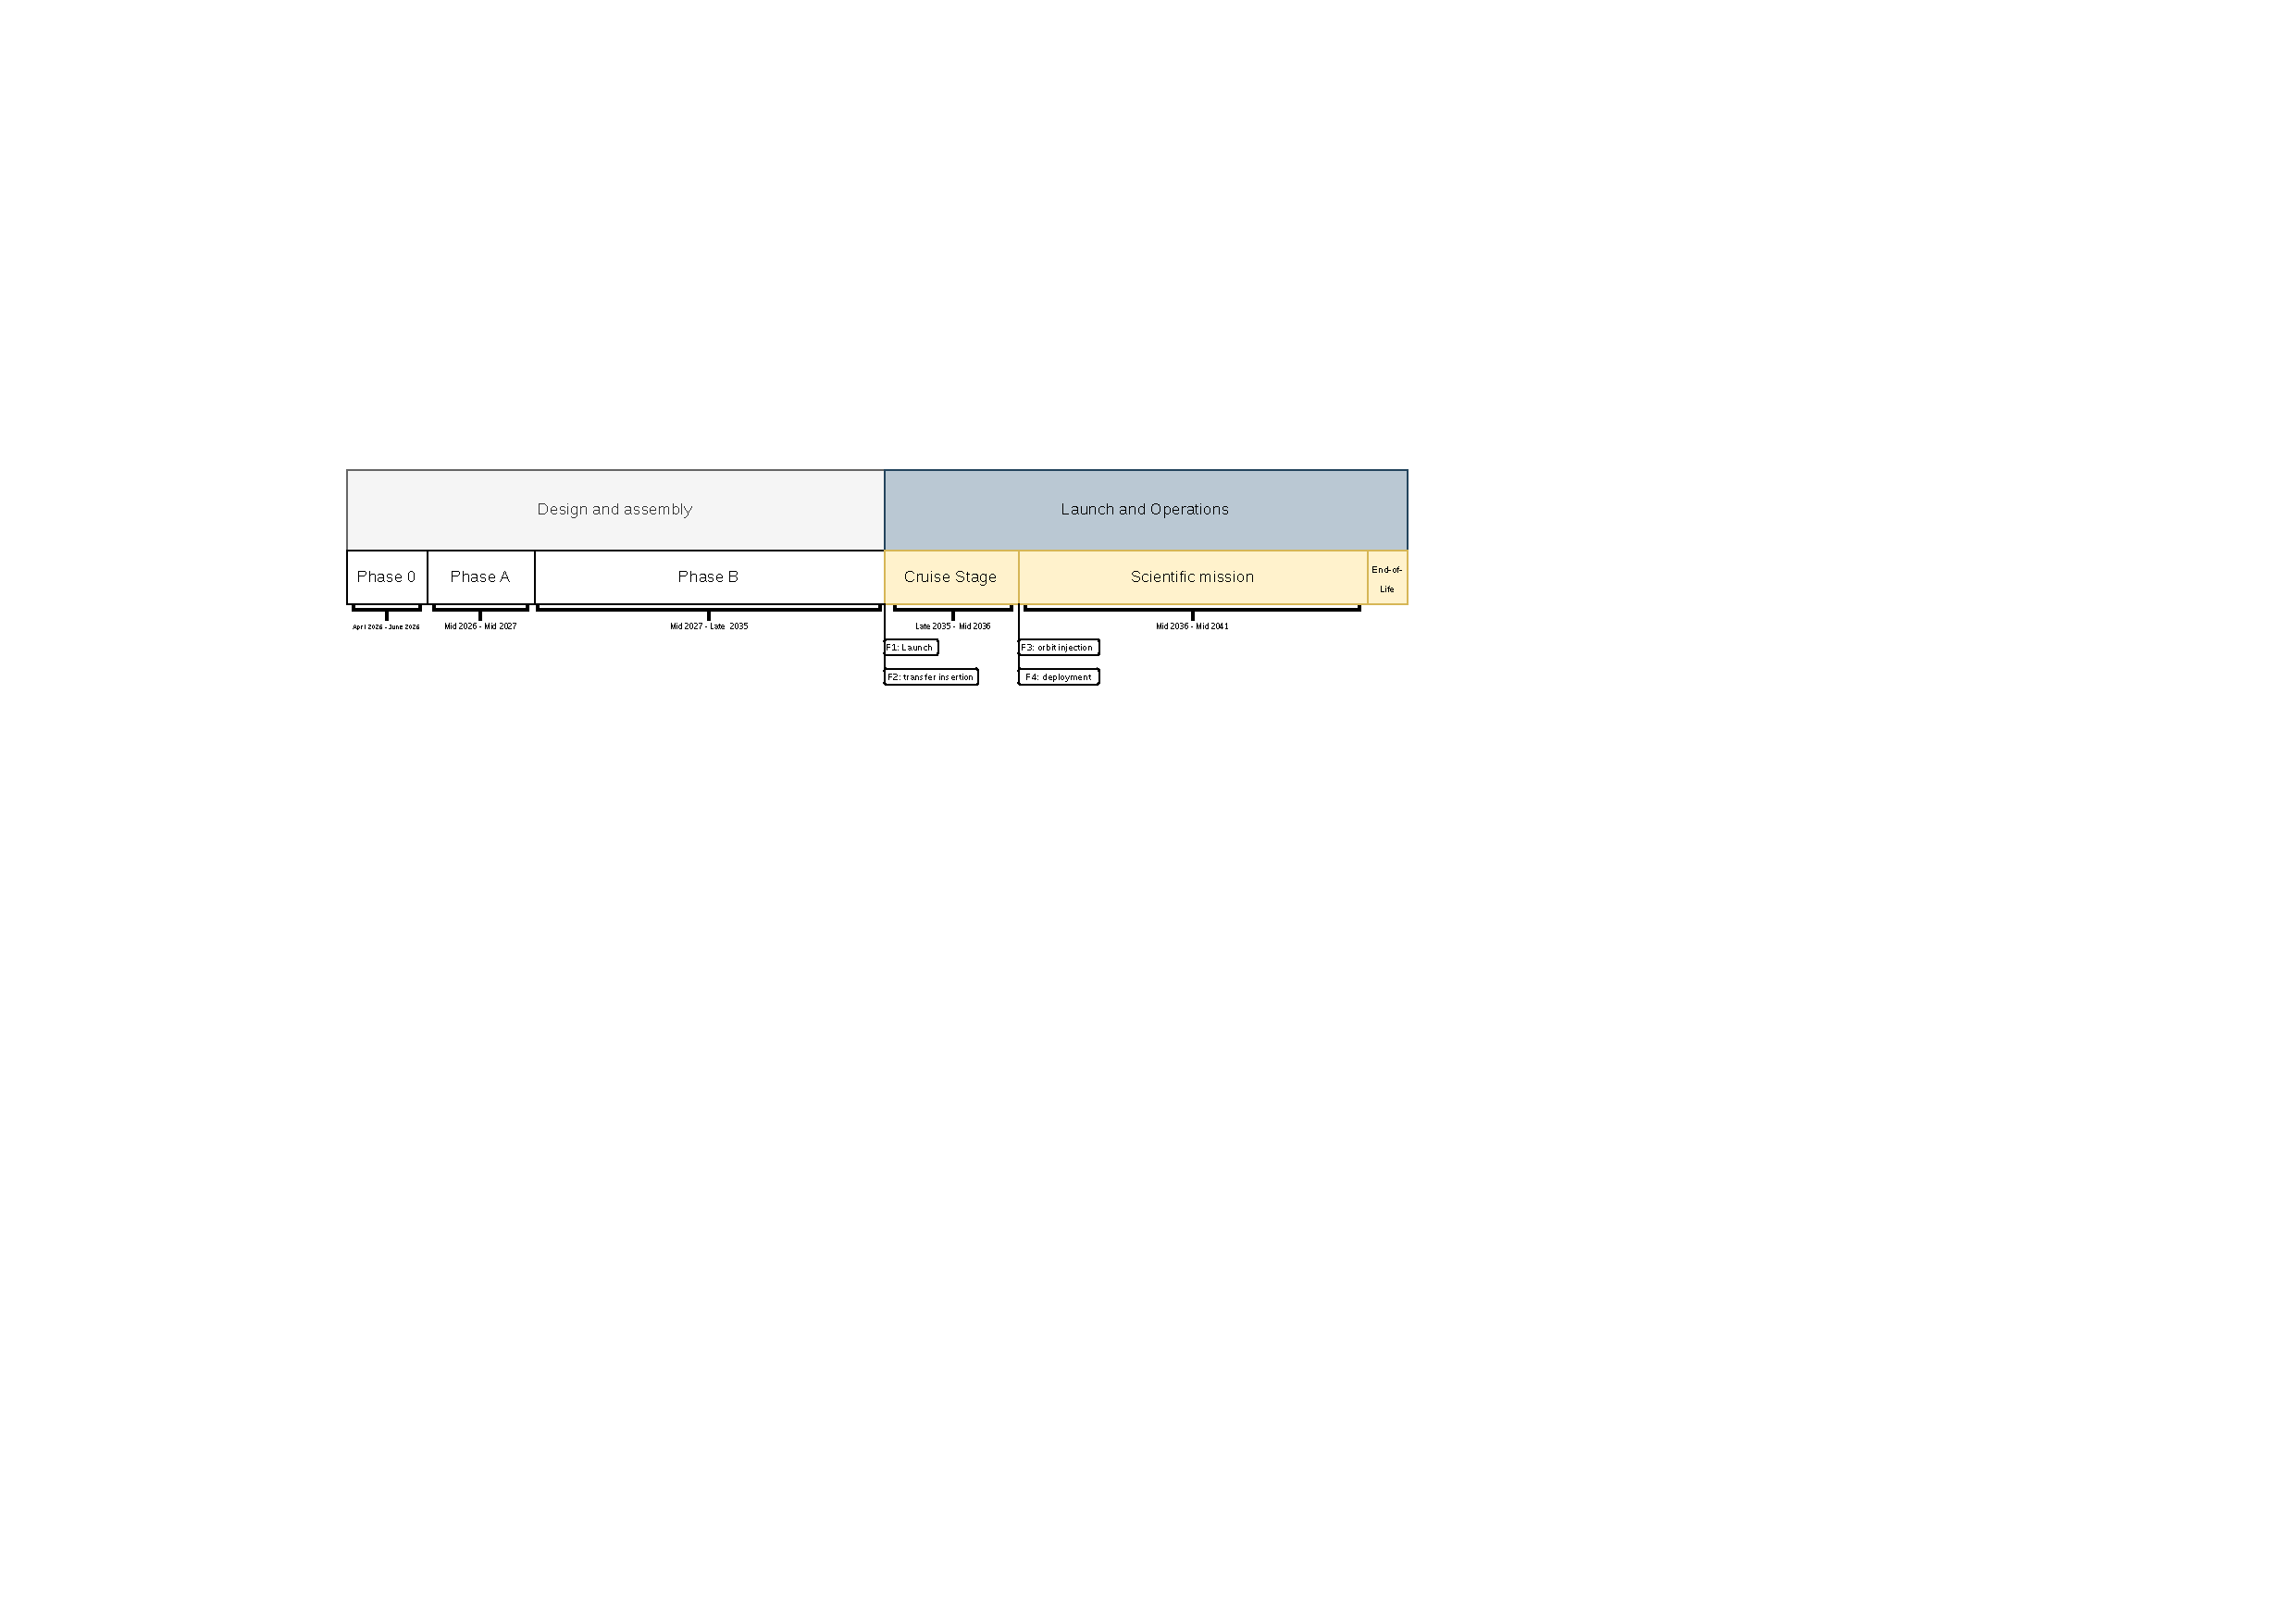
\includegraphics[width=1.2\textwidth]{fig/Operations.drawio.pdf}
    }
    \caption{Timeline}
    \label{fig:Timeline}
\end{figure}

Phase 0 sets the basic scope of the mission. For VISTA, this means defining what parts of the mission are actually designed, which include the aerobot and deployment stage, as well as verifying that the aerobot is able to perform all the required mission objectives. Other elements, such as the launcher, orbiter and ground station, are not designed in detail; however, their interfaces with VISTA are taken into consideration. Phase 0 is expected to last for the length of the DSE project.
\vspace{0.2cm}
\newline
Phase A focuses on developing the mission from an idea into a feasible concept. All mission architecture options are compared and evaluated, including the balloon architecture, in-situ resource utilization, altitude control, payload and communication strategy. The main objective of this stage is to identify a concept that is able to comply with all the requirements, while also taking into consideration and mitigating technical risks that might arise during the mission.
\vspace{0.2cm}
\newline
Phase B includes the manufacturing, assembly and testing activities, which are set to last for 8 years, until launch. At this stage, the selected VISTA concept is turned into a launch-ready system. During this stage, all subsystem layouts, mass and power budgets, the deployment sequence and verification activities are finalised. By the end of this stage, VISTA is assumed to be assembled, tested and launch-ready.






The mission operations can be seen in \autoref{fig:Con-of-op}.  
\begin{figure}[H]
    \centering
    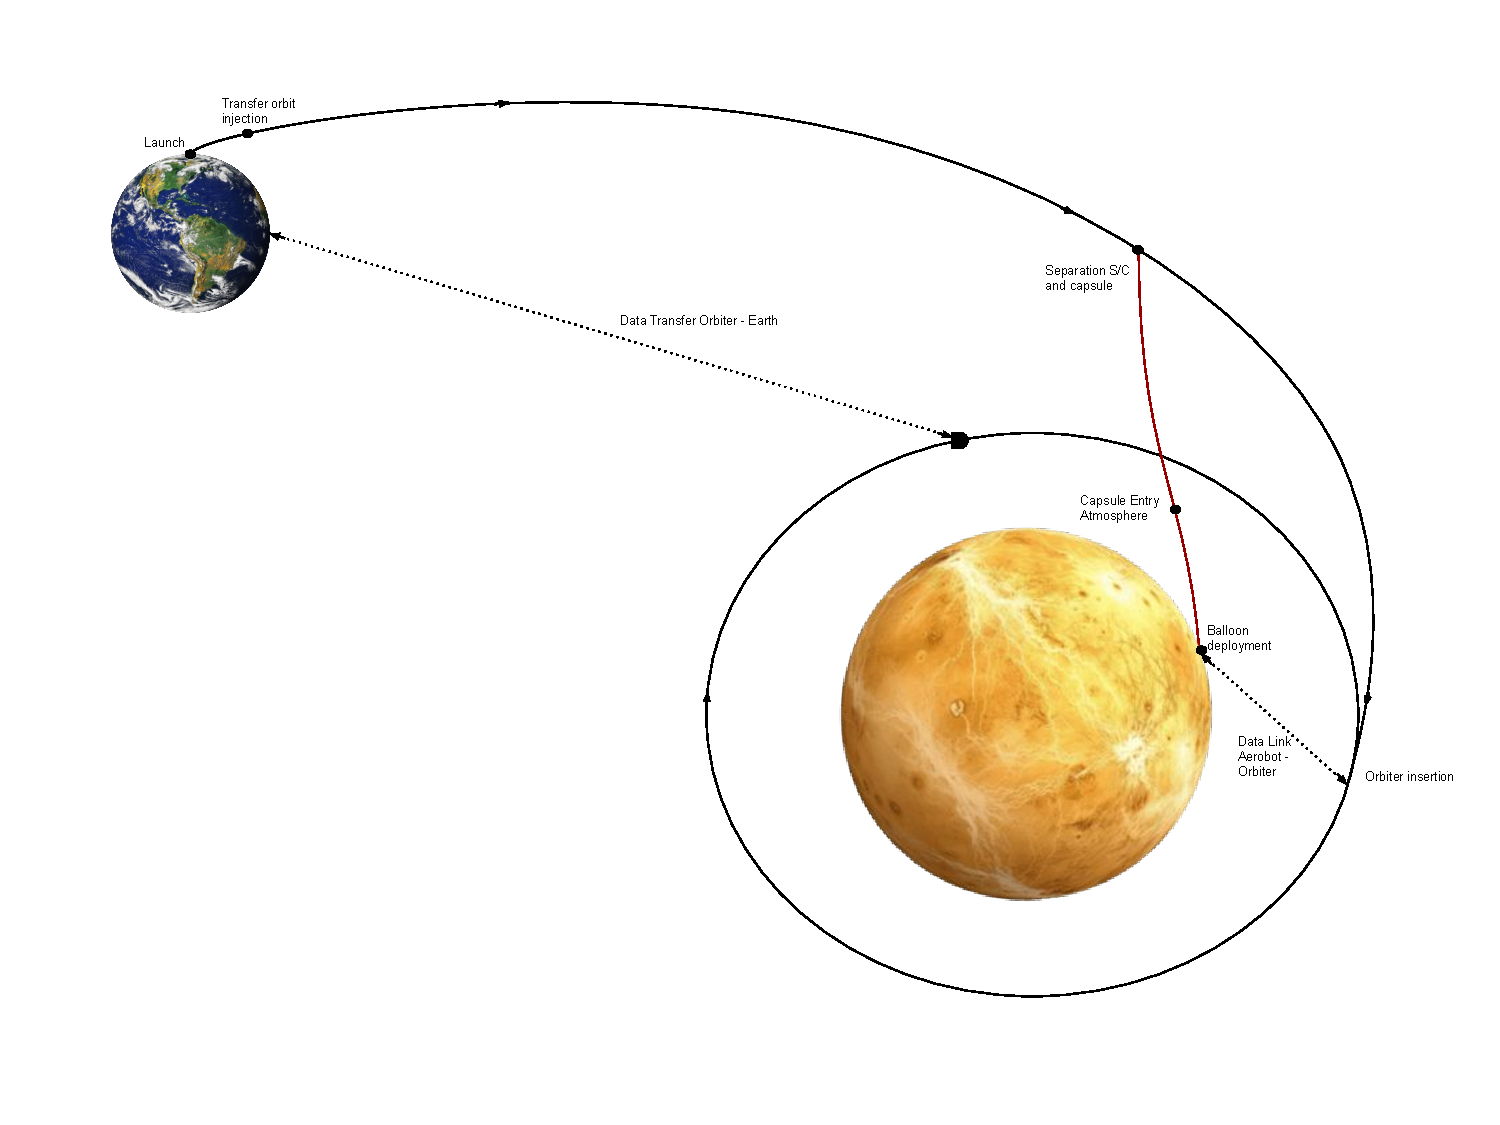
\includegraphics[width=1\linewidth]{fig/Operations.pdf}
    \caption{Concept of operation}
    \label{fig:Con-of-op}
\end{figure}
The VISTA mission follows a relay-based operational concept. After launch, the cruise stage performs the transfer to Venus while maintaining the orbiter and VISTA vehicle. Near arrival, the VISTA vehicle separates and enters the Venusian atmosphere, while the orbiter performs Venus orbit insertion. The deployment stage protects the aerobot during entry and inflation, after which the balloon-gondola system begins stable flight in the cloud layer and the deployment hardware is discarded.

During nominal operations, the aerobot performs atmospheric and seismic measurements, stores science and housekeeping data, and manages altitude through the ISRU and buoyancy subsystem. Communication relies on ESA's existing ESTRACK infrastructure, with the Venus orbiter relaying data between Mission Control and the aerobot during scheduled contact windows. At end of life, a decision is made to continue the mission or safely dispose the aerobot.






\section{Sustainability}
\label{sec:sustainability}
\todo{someone proofread pls - not too short?}

A full Life Cycle Assessment is outside the scope of the current design phase, but sustainability is considered across development, manufacturing, testing, launch, transfer, operations, and end-of-life.

The design prioritizes commercial off-the-shelf components where possible to reduce custom development effort, material waste, and manufacturing resources. Environmentally critical materials, such as high-energy batteries or acid-resistant coatings, are used only where required by the Venus environment and shall be reassessed during detailed design for lower-impact alternatives where feasible. Testing shall rely on simulations, engineering models, and combined test campaigns where possible to reduce repeated hardware production and facility use.

Since launch is expected to be a major contributor to environmental impact, spacecraft mass reduction and an efficient transfer trajectory are important mission sustainability considerations. During operations, existing and shared ground infrastructure shall be used for mission control to avoid unnecessary new facilities and reduce operational energy demand. 

At end-of-life, the aerobot is expected to remain in the Venus environment; therefore, the design shall minimize unnecessary hazardous materials, avoid avoidable contamination release, and remain compliant with applicable COSPAR planetary-protection requirements \cite{ECSS_U_ST_20C_2019} for Venus. Material choices and disposal assumptions shall be documented for future planetary-protection and end-of-life assessment.

\chapter{Trade-off}
\label{chapter: trade-off}

% Selecting the most promising design configuration is treated in two stages. In the first stage, the configurations within each subsystem are investigated and internal choices are traded-off to identify the most promising designs. The goal of this stage is to define the achievable optimal subsystem performance, given some mass, power and cost provided - this has been the subject of Chapters \ref{}-\ref{}. Afterwards, the promising subsystem options are combined into full system architectures, and those are again traded-off. Here, the overall intention is to optimize resource allocation between subsystems.

% The chapter is structured in three parts. Section~\ref{sec:coupling_map} identifies all significant cross-subsystem couplings, drawing on the N\textsuperscript{2} matrix established in Chapter~\ref{chap:n2}. Section~\ref{sec:param_coupling} quantifies the parameter-level dependencies - mass, power, volume, and reliability - with numerical values drawn directly from the subsystem chapters. Section~\ref{sec:arch_tradeoff} uses these dependencies to score three candidate system-level configurations and identifies the selected baseline together with its residual risks.

Now that all subsystem configurations have been presented, a final architecture must be selected. The configurations within each subsystem are investigated and internal choices are traded-off to identify the most promising designs. The goal of this stage was to define the achievable optimal subsystem performance, given a certain mass, power and cost provided, which has been the subject of Chapters \ref{chap:payload} to \ref{Chap: Structures}. The initial plan was to combine the most promising designs into different system architectures to be traded-off once again in order to select the final architecture. However, once the design of each subsystem was made, it was determined that there is a very limited number of possible design configurations. 

Due to the extensive list of mission requirements and the ambitious goals set for the VISTA team, as well as the harsh conditions present on Venus, many configurations were eliminated in the first (subsystem-level) stage of the trade-offs. That is, even though all subsystems internally traded-off different designs, options were eliminated due to constraints presented by other subsystems without complex system-level coupling. The N\textsuperscript{2} matrix in \autoref{chap:n2} identifies all significant cross-subsystem interface concerns that in themselves caused certain configurations to be discarded. In the following section, \autoref{sec:elimination}, the reason behind the elimination of the different concepts is explained, one by one.

After such exercise, it was concluded that there aren't enough options to construct different system architecture configurations that vary significantly enough to justify the system trade-off exercise. Therefore, for the design of the aerial balloon platform for the VISTA mission, the final selected subsystems design configurations will be combined to form the final architecture, with no system trade-off performed, only the system-level checks to ensure compatibility. 

The selected architecture will then be optimized in the next stages of the design. The final architecture is presented in \autoref{sec:final_arch}.

\section{System-Level Interfaces}\label{sec:coupling_map}
\label{sec:elimination}

The \autoref{tab:tradeoffinterfaces} below lists specific points of discussion that were raised during the subsystem design process. More precisely, it presents those that were heavily influenced by interface considerations and system-level communication between subsystem was necessary. It aims to show the extent of system-level thinking present in this project, as well as archive future potential areas for reconsideration that go beyond concepts in Chapters \ref{chap:payload} to \ref{Chap: Structures} separately.

{\footnotesize
\renewcommand{\arraystretch}{1}
\begin{longtable}{@{} p{1.8cm} p{11cm} p{2.5cm} @{}}
\label{tab:tradeoffinterfaces}

\textbf{Subsystem} & \textbf{Design options considered} & \textbf{Interface with:} \\
\midrule
\endfirsthead
\toprule
\textbf{Subsystem} & \textbf{Design options considered - kept / eliminated and why} & \textbf{Key interface} \\
\midrule
\endhead
\midrule
\multicolumn{3}{r}{\small\textit{continued on next page}} \\
\endfoot
\bottomrule
\endlastfoot

\textbf{STRUC} &
1.1. \textbf{Cube gondola - eliminated.} Flat sides allow better solar array integration. Good packing efficiency and carrier storage area occupation, however ultimately, the entry capsule is circular in shape, so any internal gains are nullified on deployment capsule packing stage.
& INSTR, EPS, DEP \\[6pt]

&
1.2. \textbf{Cylinder gondola - selected.} Better structural symmetry for pendulum stability and descent, most volume-efficient shape for deployment capsule. Solar panel integration discussed with EPS and STRUC, decided as feasible.
& DEP, ADCS, EPS, STRUC \\[6pt]

&
2.1. \textbf{Short tether - eliminated.} Balloon envelope shadows the solar panels, reducing power generation below the EPS minimum output requirement.
& EPS \\[6pt]

&
2.2. \textbf{Long tether - eliminated.} Introduces large pendulum-mode oscillations that exceed ADCS compensation authority, destabilising gondola attitude.
& ADCS \\[6pt]

&
2.3. \textbf{Medium tether - selected.} Balances solar panel clearance from balloon shadow with gondola swing dynamics within ADCS authority.
& EPS, ADCS \\[6pt]
\midrule
\textbf{INSTR} &
1. \textbf{Towbody probe - eliminated.} Tether tension loads under Venus wind shear conditions exceed the STRUC mass budget; a second independent thermal architecture for the probe would be required from TCS, making the concept infeasible within system resource allocations.
& STRUC, TCS \\[6pt]

&
2. \textbf{Gondola-only barometers (no tether) - deprioritised.} Loses directional seismic wavefront filtering; viable fallback but reduced science return, therefore retained as contingency.
& STRUC \\[6pt]

&
3. \textbf{Tethered barometer array (Architecture~B) - selected.} Barometers at 15\,m, 85\,m, and 200\,m below gondola form a vertical aperture for infrasound triangulation. GNC must supply continuous altitude state for barometric referencing; CDHS must handle the additional tether sensor data stream within its storage and downlink budget.
& GNC, CDHS \\[6pt]
\midrule
\textbf{ISRU} &
1. \textbf{Earth-sourced N\textsubscript{2} converter ($\sim$6\,kg) - eliminated.} Unit mass exceeds gondola allocation; STRUC will not accommodate it without violating the gondola mass budget for other subsystems.
& STRUC \\[6pt]

&
2.1. \textbf{Option~1 balloon (helium partial-fill + CO\textsubscript{2} ballast) - eliminated.} Initial N\textsubscript{2} fill rate requires $\sim$988\,W continuous power, exceeding the EPS budget.
& EPS \\[6pt]

&
2.2 \textbf{Option~2 balloon (pre-filled N\textsubscript{2} + PSA leakage top-up) - selected.} ISRU compensates N\textsubscript{2} leakage requiring only $\sim$21\,W continuous, compatible with EPS budget. Altitude control via internal superpressure bladder commanded by GNC, as discussed with GNC.
& EPS, GNC \\[6pt]

&
2.3. \textbf{Option~3 balloon (ISRU-only fill + disposable helium bootstrap balloon) - eliminated.} Same EPS power infeasibility as Option~1 during the fill phase; disposable helium balloon adds STRUC packaging mass and DEP sequence complexity.
& EPS, STRUC, DEP \\[6pt]
\midrule
\textbf{CDHS} &
1. \textbf{Cross-dipole antenna - eliminated.} RF power draw at required link margin exceeds the EPS power allocation for the communications subsystem and cannot be sufficiently modified with other subsystem's allocations.
& EPS \\[6pt]

&
2.1. \textbf{Single antenna - eliminated.} Cannot provide spatially separated feed points for hemispherical angular coverage. ADCS attitude determination relies on two antennas on opposite gondola edges for polarisation diversity and improved low-elevation visibility.
& ADCS \\[6pt]

&
2.2. \textbf{Two helical-ring antennas - selected.} Hemispherical coverage without cross-dipole power penalty. MSK modulation selected over BPSK for power efficiency; marginal BER trade-off at low SNR flagged to GNC as potential widening of Doppler position uncertainty at low orbiter elevation angles. Dual-antenna redundancy retained.
& EPS, GNC \\[6pt]

\midrule
\textbf{ADCS} &
1. \textbf{Continuous absolute attitude measurement - eliminated.} Data volume from continuous high-rate attitude telemetry exceeds both on-board CDHS storage capacity and the available downlink budget through the orbiter relay link.
& CDHS \\[6pt]

&
2. \textbf{IMU with periodic absolute fixes - selected.} IMU runs continuously at low data rate within CDHS storage budget; absolute corrections applied at each orbiter contact window via GNC Doppler-ranging passes. Drift errors between passes managed by anchoring at pass entry and exit boundaries.
& CDHS, GNC \\[6pt]
\midrule
\textbf{TCS} &
1. \textbf{Cryocoolers - eliminated.} Continuous cryogenic power draw incompatible with EPS budget. No allocation exists on top of ISRU, instruments, and communications demands.
& EPS \\[6pt]

&
2. \textbf{Peltier cooler (TEC) - selected for precision instrument zones.} Low power footprint acceptable within EPS allocation. Applied locally where passive control is insufficient for narrow-tolerance payload instruments.
& EPS, INSTR \\[6pt]

&
3. \textbf{Hybrid passive-active architecture - selected overall.} Passive insulation and conductive baseplates handle bulk thermal management within STRUC gondola enclosure. Active heater patches cover cold-case battery and instrument survival without exceeding the EPS nightside power budget.
& STRUC, EPS, INSTR \\[6pt]
\midrule
\textbf{EPS} &
1. \textbf{Wind turbine - eliminated.} Aerobot drifts with the zonal wind; relative wind velocity at a tether-mounted turbine is near-zero, not producing enough power to defence this mass spending to STRUC.
& STRUC \\[6pt]

&
2. \textbf{Swinging pendulum - eliminated.} Recoverable energy from gondola pendulum motion is negligible, also conflicts with ADCS requirement for minimal gondola angular disturbances.
& ADCS \\[6pt]

&
3. \textbf{Energy beamed from orbiter - eliminated.} Power delivery restricted to orbiter contact windows and requiring very precise pointing based on balloon location - not achievable by GNC. Cloud-layer attenuation and Venus-Earth pointing geometry reduce transfer efficiency to levels incompatible with continuous loads declared by ISRU.
& CDHS, GNC, ISRU \\[6pt]

&
4. \textbf{RTG alone - eliminated.} Not feasible for a Europe-based space mission, and the additional power benefits for ISRU would not be significant enough to justify switching to a USA-based mission setup.
& STRUC, EXTERNAL (Compliance) \\[6pt]

&
5. \textbf{Solar arrays + battery - primary baseline.} Solar generation sized to meet ISRU and payload requirements. Battery bridges nightside demand for ISRU, heaters, and housekeeping, within agreed mass budget allocation from STRUC. Array placement constrained by tether geometry to avoid balloon shadow.
& STRUC, ISRU, INSTR \\[6pt]

&
6. \textbf{RTG + solar hybrid - retained as fallback.} Adopted if final sizing confirms battery alone cannot bridge the nightside TCS and ISRU continuous loads. RTG mass and TCS waste-heat implications must then be re-evaluated.
& TCS, STRUC \\[6pt]
\midrule
\textbf{GNC} &
1. \textbf{Radar surface imaging - eliminated.} Radar aperture mass and volume cannot be accommodated within the STRUC gondola envelope. Continuous radar data would impose an excessive processing and storage burden on CDHS beyond its allocated capacity.
& STRUC, CDHS \\[6pt]

&
2. \textbf{Doppler tracking via relay orbiter - selected.} Provides absolute position and range-rate at each orbiter pass within the existing CDHS communication link, adding no dedicated hardware mass to STRUC. IMU propagates position between passes. Drift errors halved by anchoring at pass boundaries. MSK modulation (CDHS power constraint) introduces marginal SNR reduction widening position uncertainty at low orbiter elevation angles.
& CDHS, STRUC, ADCS \\[6pt]
\midrule
\textbf{DEP} &
1. \textbf{Deployment as independent subsystem - confirmed.} Operates autonomously through the EDLI sequence and is jettisoned before float operations; integrating deployment hardware into the float platform would add persistent dead mass penalising the STRUC gondola mass budget over the five-year mission.
& STRUC \\[6pt]

&
2. \textbf{Single-point inflation dependency - acknowledged; mitigated.} A deployment failure forfeits instruments, GNC, and ADCS entirely, motivating the $\alpha$RX-Mt3 redundancy architecture and cascaded COPV inflation string. The cascaded COPV layout was also driven by the need to provide a cross-strappable inflation path that does not compromise ISRU gas routing after float.
& INSTR, GNC, ADCS, ISRU \\[6pt]

&
3. \textbf{COPV rib structure retained post-deployment - selected.} COPVs repurposed as gondola primary structure ribs after inflation ($\varepsilon_1$ integration vector), recovering deployment hardware as useful STRUC mass rather than jettisoned deadweight.
& STRUC \\

\end{longtable}
}

% The criteria for the high-level trade-off are: Total Mass; Total Power; Total Cost. Throughout, the scoring convention mirrors that used in the subsystem chapters (Table~\ref{tab:scoring_scale}):


% \begin{table}[H]
% \centering
% \renewcommand{\arraystretch}{1}
% \caption{System-level scoring scale, consistent with subsystem trade-off methodology.}
% \label{tab:scoring_scale}
% \begin{tabular}{cl}
% \hline
% \textbf{Score} & \textbf{Meaning} \\
% \hline
% 5 & Excellent performance; no significant concern. \\
% 4 & Good performance; minor concerns manageable within current margins. \\
% 3 & Acceptable; important design concerns requiring active management. \\
% 2 & Weak performance; significant risk to mission. \\
% 1 & Very weak; high risk or architecture incompatibility. \\
% \hline
% \end{tabular}
% \end{table}



% \section{Total Cost}
% The estimated budget required for a configuration is already a quantified amount, so a comparison can be made directly. 




\section{Final Architecture}
\label{sec:final_arch}

Due to the aforementioned reasons, the final architecture will be comprised of the selected configurations of each respective subsystem. It is important to note that already on subsystem level, or with decoupled communication between pairs of subsystems without engagement of multiple complex system-wide roles, the design options have been eliminated to only one per subsystem. The reason for such occurrence is the challenging profile of the mission of interest - most subsystem configurations were discarded early on due to inapplicability to project's limited budgets, unique approaches (such as active replenishment system) and demanding requirements.

The resulting architecture integrates a gondola, a buoyancy management system, a distributed science payload, and supporting avionics subsystems into a single coherent float platform.

\subsubsection*{Gondola and Structure}
The primary structure takes the form of a cylindrical gondola, chosen for the structural symmetry it provides for pendulum stability during float and efficient volume usage within deployment capsule. The gondola is suspended 15 m below the balloon envelope, a tether length selected to balance solar panel clearance from balloon shadow against acceptable gondola swing dynamics. Following atmospheric entry and descent, the COPV rib structure from the deployment stage is retained and incorporated into the gondola's primary structure, recovering descent hardware as useful structural mass.

\subsubsection*{Balloon and Buoyancy Management}
Buoyancy is maintained through a pre-filled N$_2$ balloon architecture augmented by a Pressure Swing Adsorption system that compensates for slow daily envelope leakage. This approach was selected as the only configuration compatible with the mission power budget; alternatives relying on large-scale in-situ gas generation or disposable helium balloons were eliminated on grounds of power infeasibility or excessive mass.

\subsubsection*{Science Payload}
The gondola carries a suite of nine instruments targeting atmospheric composition, dynamics, cloud microphysics, and radiative flux. A Neutral Mass Spectrometer characterises bulk atmospheric composition, while a miniature Tunable Laser Spectrometer provides complementary trace gas measurements. Cloud and aerosol properties are measured by an Aerosol Fine-mode spectrometer and an Optical Particle Counter. Atmospheric dynamics are captured through a Wind Instrument System and a Sonic Anemometer providing direct in-situ wind vector measurements. Two pyrgeometers measure upward and downward longwave radiative fluxes, and a TOPS sensor characterises atmospheric optical properties.
Pressure measurements are made by an array of five barometers distributed across a vertical tethered structure suspended beneath the gondola, with sensors positioned at 15 m, 85 m, and 200 m below the gondola baseline. This vertical aperture, referred to as Architecture B, enables directional seismic wavefront filtering and spatial pressure gradient measurements that a gondola-only barometer configuration could not provide. The navigation subsystem supplies continuous altitude state to the array, and the data handling subsystem manages the resulting multi-stream sensor data.

\subsubsection*{Power System}
The platform is powered primarily by solar arrays generating power during the Venusian day, supported by a battery for night-side energy storage. Wind energy harvesting and orbiter-beamed power were both eliminated as viable options; the former because the aerobot drifts with the ambient wind leaving no exploitable relative velocity at a turbine, and the latter due to the combined constraints of intermittent orbiter contact windows and cloud-layer attenuation.
Thermal Control
Thermal management follows a hybrid passive-active architecture. Passive insulation and conductive baseplates handle the bulk of heat management across the gondola structure. A Palantir Peltier-based cooler provides active precision temperature control in zones housing instruments whose operational requirements exceed what passive management alone can maintain. Active heater patches supplement the system in cold-case conditions, providing survival-level heating to the battery and critical instruments.

\subsubsection*{Attitude Determination, Navigation, and Communications}
Attitude determination is performed by an IMU operating continuously at a low data rate, with periodic absolute corrections applied during relay orbiter contact windows via Doppler-ranging passes. This approach was selected over continuous absolute attitude measurement, which would have generated data volumes exceeding both onboard storage capacity and downlink budget.
Navigation relies on the same Doppler-tracking infrastructure, with the relay orbiter providing absolute position and range-rate at each contact pass. The IMU propagates the platform's position between passes, with accumulated drift errors anchored at each pass boundary. It is noted that the MSK modulation scheme adopted for the communications subsystem introduces a marginal signal-to-noise trade-off that slightly widens position uncertainty at low orbital elevation angles.
Communications are handled by two helical-ring antennas mounted on opposite gondola edges, providing hemispherical coverage and polarisation diversity without the power penalty associated with a cross-dipole configuration. MSK modulation was selected for its power efficiency, with a small bit-error-rate trade-off relative to BPSK acknowledged. The dual-antenna architecture additionally provides a redundant communication path in the event of a deployment stage jettison failure.

\subsubsection*{Entry, Descent, and Deployment}
The deployment subsystem operates as an independent unit, functioning autonomously through the entry, descent, and inflation phase before being jettisoned ahead of the float mission. Decoupling deployment from the float platform avoids carrying persistent descent hardware mass through the five-year operational lifetime. The single-point dependency that deployment success represents for the payload, navigation, and attitude determination subsystems is acknowledged, and motivates the $\alpha$RX-Mt3 redundancy architecture and cascaded COPV inflation string incorporated into the deployment design.


\section{Sensitivity Analysis}

no sensivty lmaao

%TCS SCRATCHED OFF CRYOCOOLERS BECAUSE OF too much POWER from EPS

%dome-gondola connection: long lines - too much mass mass (affects STRUC) and oscillation (affects ADCS) but short lines (EPS) dome makes solar panels overshadowed (EPS)

%GNC - radar tracking scratched bcs radar too requiring from PAYLOAD subsystem (no place for it) 

%CDHS - cross dipole antenna cant be used bcs too much power required from EPS. plus CDHS uses minimum shift keying bcs its more power efficient, but lower reliability (GNC affected)

%CDHS - one antenna not possible bcs ADCS needs two antennas for dipole 

%STRUC layout : PAYLOAD scratches off the configuration that doesnt have enough opening for payloads to collect measurements

%PAYLOAD scratched off towbody because its too heavy (it would affect STRUC badly, also TCS because towbody would have thermal control too)

%PAYLOAD consideration: barometers on wire need altitude input - GNC challenge/CDHS affected 

%ADCS: conf with always absolute measurement scratched from CDHS, as its not possible too much data. so IMU with only absolute fixes once in a while,only marginal effect on STRUC (extra mass)

%ISRU - Earth 6kg converter - too heavy (STRUC)

%CDHS - redundancy for antenna if DEPLOYMENT fails











\chapter{Verification \& Validation Procedures}

The verification and validation (V\&V) programme for the Venus aerial balloon platform is structured in accordance with the European Cooperation for Space Standardization standard ECSS-E-ST-10-02C Rev.1 \cite{ECSS_VER} and its companion handbook ECSS-E-HB-10-02A \cite{ECSS_HB}. In the ECSS framework, verification demonstrates that the delivered system meets its specified requirements, while validation confirms that those requirements correctly address the mission's intended use. 

The V\&V process is structured around three sequential activities: verification planning, verification execution and reporting, and verification control and close-out. Planning is conducted top-down from mission-level requirements to system requirements. Meanwhile, execution and reporting proceeds bottom-up from component acceptance through system qualification. 
% No verification and validation will be performed in this phase of the design, as this falls out of the scope of this feasibility study. 

\section{Verification Approach}

Per ECSS-E-ST-10-02C, four verification methods are available and are applied to each system requirement of the VISTA mission:

\begin{itemize}[itemsep=1pt, parsep=1pt]
    \item Test (T): Measurement of product performance and functions under representative simulated environments. Test is the preferred method as it provides the highest confidence in verification of performance and design. All safety-critical requirements must be verified by test.
    \item Analysis (A): Theoretical or empirical evaluation using agreed analytical techniques, including computational simulation and modelling. Analysis is used where full flight conditions cannot be simulated on the ground, or where testing the full spectrum of conditions is not economically feasible.
    \item Review of Design (R): Use of approved records and evidence from past missions and design documents that unambiguously demonstrate a requirement is met.
    \item Inspection (I): Visual determination of physical characteristics. 
\end{itemize}

% For any requirement verified solely by Analysis or Review of Design, a risk assessment is conducted to determine whether the impact on the mission is major or minor. Where the impact is judged major, a cross-check using two independent analyses from separate teams and models is required as part of the Verification Plan.

Verification is conducted at three levels: equipment level, subsystem level, and system level. The V\&V plan at subsystem level is presented at their corresponding subsystem chapter. For this chapter, only system level testing will be considered. That is, the V\&V plan for the fully integrated gondola platform, including the balloon envelope, tethered barometer array, and all deployed interfaces.

\section{Verification Model Philosophy}

The model philosophy defines the optimum set of physical models required to achieve confidence in the product verification, balancing cost, schedule, and risk. For the Venus aerial balloon platform, a hybrid model philosophy is adopted, comprising three model types:

\begin{enumerate}[itemsep=1pt, parsep=1pt]
    \item Engineering Model (EM): Flight representative in form and function - the difference with respect to the Flight Model is lack of high-reliability parts and no full redundancy. Used for functional qualification, interface verification, failure survival demonstrations, and to validate ground support equipment and test facilities. The EM is also used to develop and validate the software verification environment before integration onto the PFM.
    \item Structural-Thermal Model (STM): Combines the objectives of the Structural Model and Thermal Model. Fully representative of the mechanical and thermal properties of the gondola platform. Used for qualification of the structural design under launch loads and the thermal design under Venus float hot and cold cases, and for correlation of finite element and thermal mathematical models. The STM comprises a representative structure equipped with mass and thermal dummies of flight equipment.
    \item Protoflight Model (PFM): The flight end product, on which a protoflight qualification and acceptance test campaign is performed before flight. This is applicable to all levels of the system. 
\end{enumerate}

This hybrid approach is selected because it permits advanced structural and thermal qualification on the STM in parallel with functional development on the EM, reducing schedule risk, while the protoflight approach on the PFM avoids the cost of a separate dedicated qualification model. 

% The model philosophy is summarised in Table~\ref{tab:model_philosophy}.

% \begin{table}[H]
% \centering
% \caption{Summary of model philosophy for the Venus aerial balloon platform.}
% \label{tab:model_philosophy}
% \renewcommand{\arraystretch}{1.3}
% \begin{tabular}{llll}
% \toprule
% \textbf{Model} & \textbf{Primary Objective} & \textbf{Test Programme} & \textbf{Utilisation} \\
% \midrule
% EM  & Functional qualification, I/F verification & Functional, EMC & Ground support \\
% STM & Structural and thermal qualification & Vibration, shock, TVac & Disposal post-test \\
% PFM & Protoflight qualification + flight use & Protoflight, acceptance & Flight \\
% \bottomrule
% \end{tabular}
% \end{table}

\section{System-Level Test Campaign}

The system-level test campaign is conducted on the STM and PFM in sequential phases. All equipment and subsystem qualification must be completed before system-level testing commences. The main system-level test events are described in the following subsections.

\subsection{Structural, Mechanical, and Thermal Balance Tests (STM)}

The STM undergoes a full structural qualification test campaign. Launch vibration loads are applied to the gondola primary structure including the tether attachment interface, instrument mounting points, and the rib structure retained from the deployment stage. Acoustic and shock tests are conducted to qualify the gondola against the launch environment of the target launcher. Structural margins are verified against requirements REQ-C-LAU-01 and REQ-C-LAU-02. The STM is also used to validate the GSE handling interfaces and integration procedures.

% The test programme covers the Venus float hot case (52\,km, maximum solar input, maximum instrument dissipation) and the cold case (62\,km, night side, minimum power). As noted by 
Lorenz~\cite{Lorenz2018}, planetary in-situ test environments cannot fully replicate target atmospheric conditions on the ground; the thermal-vacuum test therefore targets the dominant thermal phenomena - absorbed solar flux, internal dissipation, and radiative exchange - at representative pressure levels approximating 52-62\,km Venus conditions, rather than attempting full atmospheric composition replication. In-flight thermal anomalies are generally attributable to differences between static test chamber conditions and dynamic flight conditions rather than to atmospheric composition \cite{Lorenz2018}. The thermal mathematical model is correlated against the STM test results and used to predict in-flight performance. This campaign verifies requirements REQ-C-ENV-01, REQ-C-ENV-02, REQ-F-ENV-03, and REQ-F-ENV-04.

\subsection{Functional and Electromagnetic Compatibility Tests (EM)}

The Engineering Model undergoes a full functional qualification campaign covering all nominal and redundant operational modes. Interface verification is conducted between all subsystems at the system level: the dual helical-ring antenna chain (transmit/receive), the IMU/ADCS chain with simulated Doppler-ranging inputs, the PSA leakage top-up control loop, and the instrument data acquisition pipeline from all nine science instruments. Electromagnetic compatibility testing verifies that the dual helical-ring antenna architecture does not produce mutual interference, and that no instrument is degraded by the communications subsystem. Software is verified in the target hardware environment on the EM in accordance with ECSS-E-ST-40. End-to-end communication chain testing with a simulated relay orbiter contact is conducted to verify REQ-C-SUB-05.

\subsection{Entry, Descent, and Deployment Test (PFM)}

The DEP subsystem is an independent unit that operates autonomously through the EDLI phase before jettison. Because deployment failure forfeits the entire platform, the deployment sequence is a safety-critical function and \emph{must} be verified by test. The protoflight test campaign includes a full deployment sequence test exercising the cascaded COPV inflation string and the $\alpha$RX-Mt3 redundancy architecture, verifying balloon envelope deployment without tearing, snagging, or entanglement in accordance with REQ-F-DEP-03. Dynamic stability during re-entry is verified per REQ-F-DEP-08, and structural integrity under re-entry loads is verified per REQ-C-DEP-07. The launch-locking mechanism release sequence is tested per REQ-F-LAU-05, which carries a red-flag safety-critical designation in the requirements baseline.

\subsection{Earth Stratospheric Analogue Flight (PFM)}

Following terrestrial qualification, a reduced-scale Earth stratospheric balloon flight is conducted to validate system-level float performance in an environment approximating the temperature and density of the Venus middle cloud layer. This approach follows the precedent established by the JPL Venus aerobot prototype flights, in which a one-third scale platform was flown over Nevada's Black Rock Desert to altitudes replicating the conditions expected at 55\,km above Venus~\cite{JPL2022}. The analogue flight validates: float altitude stability, tether pendulum dynamics of the barometer array under realistic atmospheric turbulence, solar array power generation under flight conditions, and instrument data acquisition in a dynamically floating platform environment. GNC position propagation between simulated relay orbiter passes is also validated by recording the full IMU data stream and applying the Doppler anchoring algorithm in post-processing.

\section{Verification Control Document}

The Verification Control Document (VCD) is the master tracking matrix that records, for each system-level requirement: the requirement text, the assigned verification method(s), the model on which verification is performed, the applicable verification stage, references to the evidence documents (test reports, analysis reports, review-of-design reports, inspection reports), the compliance status, and the close-out status. The VCD is initialised at Phase~B and maintained throughout the project life cycle until final close-out is approved by the Verification Control Board.

Table~\ref{tab:vcd} presents the initial issue of the system-level VCD for the Venus aerial balloon platform, covering all annotated requirements from the mission requirements baseline.

\newcommand{\crit}{\cellcolor{red!20}}

{\small
\renewcommand{\arraystretch}{1}
\begin{longtable}{p{2.85cm} p{6.2cm} p{1.2cm} p{1.6cm} p{1.8cm}}
\caption{System-level Verification Control Document (initial issue). Red shading denotes safety-critical requirements that must be verified by test. Methods: T = Test, A = Analysis, R = Review of Design, I = Inspection.}
\label{tab:vcd} \\
\toprule
\textbf{Req. ID} & \textbf{Requirement} & \textbf{Method} & \textbf{Model} & \textbf{Stage} \\
\midrule
\endfirsthead
\multicolumn{5}{c}{\tablename\ \thetable{} - continued}\\
\toprule
\textbf{Req. ID} & \textbf{Requirement} & \textbf{Method} & \textbf{Model} & \textbf{Stage} \\
\midrule
\endhead
\midrule
\multicolumn{5}{r}{\textit{Continued on next page}}\\
\endfoot
\bottomrule
\endlastfoot

\multicolumn{5}{l}{\textbf{Mission Requirements}} \\
\midrule

REQ-C-MIS-01 & The aerobot operational lifetime shall be at least 5 Earth years. & \textbf{A} & EM, PFM & Qualification \\
REQ-C-MIS-02 & Total aerobot system mass shall not exceed 700\,kg. & \textbf{I} & PFM & Acceptance \\
REQ-C-MIS-03 & Each aerobot shall have a survival probability greater than 90\% over the 5-year mission. & \textbf{A} & EM & Qualification \\
REQ-F-MIS-04 & The design shall incorporate the use of atmospheric nitrogen to compensate for helium leakage. & \textbf{R} & - & Qualification \\
REQ-C-MIS-05 & All subsystems shall have a minimum Technology Readiness Level of 4. & \textbf{R} & - & Qualification \\
REQ-C-MIS-06 & The aerobot shall be able to adjust its operating altitude at a rate of TBD. & \textbf{A} & EM, PFM & Qualification \\

\midrule
\multicolumn{5}{l}{\textbf{Launch Requirements}} \\
\midrule

REQ-C-LAU-01 & The S/C shall be compatible with TBD loads involved in launch. & \textbf{T} & STM & Qualification \\
REQ-C-LAU-02 & The S/C shall be compatible with TBD vibrations involved in launch. & \textbf{T} & STM & Qualification \\
REQ-C-LAU-03 & The S/C shall be compatible with the TBD volume envelope of the launcher. & \textbf{I} & PFM & Acceptance \\
REQ-F-LAU-04 & The balloon inflation and deployment mechanism shall not be activated before Venus entry. & \textbf{T}, \textbf{R} & PFM & Qualification, Pre-launch \\
\crit REQ-F-LAU-05 & \crit All launch-locking mechanisms shall be released after arrival at Venus without preventing deployment. & \crit\textbf{T} & \crit PFM & \crit Qualification \\
\crit REQ-F-LAU-06 & \crit Pre-launch integration tests shall be performed to verify the interfacing compatibility of the capsule, launcher, spacecraft, and aerobot. & \crit\textbf{T} & \crit PFM & \crit Pre-launch \\

\midrule
\multicolumn{5}{l}{\textbf{Balloon Entry and Deployment Requirements}} \\
\midrule

REQ-F-DEP-01 & The aerobot(s) shall be compatible with deployment from a Venus orbiter with a 24-hour elliptical orbit acting as a data relay. & \textbf{R} & - & Qualification \\
REQ-C-DEP-02 & The aerobot(s) shall be deployable to an operational altitude of TBD\,km. & \textbf{I} & PFM & Qualification \\
\crit REQ-F-DEP-03 & \crit The balloon envelope shall deploy without tearing, snagging, or entanglement with the gondola, parachute, or aeroshell. & \crit\textbf{T} & \crit PFM & \crit Qualification \\
REQ-F-DEP-04 & The aerobot(s) shall support post-deployment status assessment and confirmation of successful deployment. & \textbf{T} & PFM & Qualification, Commissioning \\
REQ-C-DEP-06 & The aerobot shall not vent at least TBD\% of stored TBD gas into the balloon before reaching TBD altitude. & \textbf{A} & PFM & Qualification \\
\crit REQ-C-DEP-07 & \crit The system shall sustain at least all the TBD loads experienced during re-entry. & \crit\textbf{T} & \crit STM & \crit Qualification \\
REQ-F-DEP-08 & The system shall ensure dynamic stability of the aerobot during re-entry and deployment. & \textbf{T} & PFM & Qualification \\
REQ-F-DEP-09 & The aerobot and all supporting systems shall be compatible with the dimensional constraints of the entry capsule. & \textbf{I} & PFM & Acceptance \\

\midrule
\multicolumn{5}{l}{\textbf{Sub-system Budget Requirements}} \\
\midrule

REQ-C-SUB-01 & Gondola mass shall not exceed 200\,kg. & \textbf{I} & PFM & Acceptance \\
REQ-C-SUB-02 & Balloon envelope mass shall not exceed 100\,kg. & \textbf{I} & PFM & Acceptance \\
REQ-C-SUB-03 & Inflation system mass shall not exceed 150\,kg. & \textbf{I} & PFM & Acceptance \\
REQ-C-SUB-04 & Aeroshell and parachute mass shall not exceed 250\,kg. & \textbf{I} & PFM & Acceptance \\
REQ-C-SUB-05 & Data transmission rate shall not exceed 1500\,bps. & \textbf{T} & EM & Qualification \\
REQ-C-SUB-06 & Total onboard energy storage shall not exceed 500\,Wh. & \textbf{T} & EM, PFM & Qualification, Acceptance \\
REQ-C-SUB-07 & The balloon leakage shall be no more than TBD\,cm\textsuperscript{3}\,m\textsuperscript{-2}\,day\textsuperscript{-1}. & \textbf{T} & PFM & Qualification \\

\midrule
\multicolumn{5}{l}{\textbf{Science Requirements}} \\
\midrule

REQ-F-SCI-01 & The system shall perform aerosol sampling and detailed chemical analysis of clouds at least once per month. & \textbf{R} & - & Qualification \\
REQ-F-SCI-02 & The sampling system shall not affect the chemical composition of the sample. & \textbf{T} & EM & Qualification \\
REQ-C-SCI-03 & The maximum altitude separation between samples shall be TBD\,km. & \textbf{R} & - & Qualification \\
REQ-C-SCI-04 & The altitude accuracy of sampling shall be TBD\,km. & \textbf{T} & EM, PFM & Qualification \\
REQ-C-SCI-05 & The S/C shall be able to measure vertical wind speed at TBD intervals. & \textbf{R} & - & Qualification \\
REQ-F-SCI-06 & The S/C shall include TBD measurement systems to detect any seismic activity. & \textbf{R} & - & Qualification \\
REQ-F-SCI-07 & The S/C shall be able to measure cloud dynamics at TBD intervals. & \textbf{R} & - & Qualification \\
REQ-F-SCI-08 & The S/C shall be able to measure horizontal wind speed at TBD intervals. & \textbf{R} & - & Qualification \\
REQ-F-SCI-09 & The mission shall address the VEXAG roadmap goals. & \textbf{R} & - & Qualification \\
REQ-F-SCI-10 & The S/C shall be able to measure the temperature of the Venusian atmosphere. & \textbf{T} & EM, PFM & Qualification, Commissioning \\
REQ-F-SCI-11 & The S/C shall be able to measure the pressure of the Venusian atmosphere. & \textbf{T} & EM, PFM & Qualification, Commissioning \\

\midrule
\multicolumn{5}{l}{\textbf{Survive Operating Environment}} \\
\midrule

\crit REQ-C-ENV-01 & \crit The aerobot shall tolerate the range of atmospheric pressure of TBD-TBD\,Pa. & \crit\textbf{T} & \crit STM, PFM & \crit Qualification \\
\crit REQ-C-ENV-02 & \crit The aerobot shall tolerate the atmospheric temperature range of TBD-TBD\,K. & \crit\textbf{T} & \crit STM, PFM & \crit Qualification \\
REQ-F-ENV-03 & The aerobot(s) properties shall not degrade more than TBD\% in TBD years in Venus' toxic atmosphere. & \textbf{A} & EM & Qualification \\
REQ-F-ENV-04 & The aerobot shall withstand the TBD radiation experienced during the entire mission duration. & \textbf{A} & - & Qualification \\

\midrule
\multicolumn{5}{l}{\textbf{External Compliance Requirements}} \\
\midrule

REQ-OP-COMP-01 & The mission shall comply with COSPAR planetary protection guidelines regarding atmospheric contamination. & \textbf{R} & - & Qualification \\
REQ-C-COMP-02 & Total mission cost shall not exceed 400 million euros in FY2026, including operations. & \textbf{R} & - & Qualification \\
REQ-C-COMP-03 & The S/C shall fit inside the required launch window of late 2035-2037. & \textbf{R} & - & Qualification \\
REQ-OP-COMP-04 & The mission shall comply with the Outer Space Treaty requirements regarding the harmful contamination of celestial environments. & \textbf{R} & - & Qualification \\
REQ-OP-COMP-05 & The mission shall define an end-of-life procedure to avoid harmful contamination of the Venus atmosphere. & \textbf{R} & - & Qualification \\
REQ-OP-COMP-07 & All components shall be compatible with what the available contractors can deliver. & \textbf{R} & - & Qualification \\
REQ-F-COMP-05 & The project shall identify a qualified backup manufacturer for all mission-critical manufactured components before the start of final production. & \textbf{R} & - & Qualification \\

\midrule
\multicolumn{5}{l}{\textbf{Payload Requirements}} \\
\midrule

REQ-C-PAY-01 & Each instrument suite shall achieve a successful analysis probability greater than 80\%. & \textbf{T} & EM, PFM & Qualification, Commissioning \\
REQ-C-PAY-02 & The total mass of the payload shall stay below TBD\,kg. & \textbf{I} & PFM & Acceptance \\
REQ-F-PAY-03 & Scientific components shall fit within the TBD volume of the allocated space. & \textbf{I} & PFM & Acceptance \\
REQ-F-PAY-04 & The generated payload data that needs to be stored shall be no more than TBD\,MB. & \textbf{T} & EM & Qualification \\

\end{longtable}
}

\section{Verification Rationale for Key Requirements}

Several requirements warrant explicit justification for the chosen verification method, particularly those verified by Analysis alone and those carrying a safety-critical designation.

\subsection{REQ-C-MIS-01 and REQ-C-MIS-03 - 5-Year Lifetime and Survival Probability}

A 5-year operational lifetime at Venus cannot be verified by direct test in a reasonable programme schedule. Verification is therefore assigned to Analysis, combining: (i) accelerated balloon envelope leakage testing at elevated temperatures to project long-term degradation; (ii) PSA system endurance modelling at the required 20-22\,g/day leakage compensation rate; (iii) fault tree analysis and reliability modelling to derive the survival probability estimate. Because the impact of failing these requirements on the mission is major, an independent cross-check analysis using a second team and independent models is mandatory per ECSS-E-ST-10-02C clause 5.2.2.1.

\subsection{REQ-F-ENV-03 and REQ-F-ENV-04 - Atmospheric Degradation and Radiation Tolerance}

Full replication of Venus atmospheric conditions - including sulphuric acid aerosol chemistry at 0.5\,bar and 52-62\,km equivalent temperature - is not achievable in a standard ground test facility. As Lorenz~\cite{Lorenz2018} demonstrates, it is physically impossible to achieve all environmental parameters simultaneously at affordable cost, and careful analytical methods validated against available data provide the appropriate approach. Verification is therefore by Analysis, supported by materials compatibility test data from component-level testing and published Venus exploration heritage data. The analytical models are validated against VEGA balloon mission heritage where applicable.

\subsection{REQ-C-MIS-06 - Altitude Adjustment Rate}

Altitude control authority is a function of the PSA top-up rate, ballast capacity, and atmospheric density gradients. Verification by Analysis using the validated altitude control model is appropriate. The Earth stratospheric analogue flight provides a complementary empirical data point on achievable altitude change rates.

\subsection{Safety-Critical Requirements}

The following requirements are designated safety-critical in the requirements baseline (indicated by red highlighting) and are therefore mandated to be verified by Test under ECSS-E-ST-10-02C clause 5.2.2.1(b). No waiver or substitution by Analysis alone is permissible:

\begin{itemize}[itemsep=1pt, parsep=1pt]
    \item \textbf{REQ-F-LAU-05} - launch-locking mechanism release: verified by functional actuation test on the PFM at representative Venus-transit thermal conditions.
    \item \textbf{REQ-F-LAU-06} - pre-launch integration compatibility: verified by a full system-level integrated test on the PFM at the launch site prior to encapsulation.
    \item \textbf{REQ-F-DEP-03} - balloon envelope deployment without tearing: verified by a full deployment sequence test on the PFM, exercising the complete COPV inflation cascade and $\alpha$RX-Mt3 redundancy chain.
    \item \textbf{REQ-C-DEP-07} - re-entry structural loads: verified by structural load testing on the STM to the required qualification margins over the predicted re-entry load spectrum.
    \item \textbf{REQ-C-ENV-01 and REQ-C-ENV-02} - atmospheric pressure and temperature tolerance: verified by thermal-vacuum testing on the STM and PFM across the defined qualification temperature and pressure range for the Venus middle cloud layer environment.
    \item \textbf{REQ-STK-1.7} - survive the operating environment of Venus: this top-level stakeholder requirement is closed out by the combined evidence of REQ-C-ENV-01, REQ-C-ENV-02, REQ-F-ENV-03, and REQ-F-ENV-04, with test evidence being a mandatory constituent.
\end{itemize}

\section{Verification Process Phasing}

The verification programme is phased with the project life cycle in accordance with ECSS-M-ST-10. The key milestones and verification deliverables are:

\begin{itemize}[itemsep=1pt, parsep=1pt]
    \item \textbf{Phase~A (PRR):} Initial verification approach defined; preliminary model philosophy proposed; requirement criticality assessment initiated.
    \item \textbf{Phase~B (SRR/PDR):} Verification Control Document initialised with verification matrix; all system-level requirements assigned methods, levels, and stages; test feasibility confirmed; VCD and preliminary Verification Plan issued.
    \item \textbf{Phase~C (CDR):} Verification Plan completed and frozen; analysis and Review-of-Design activities completed at lower levels; STM integration commenced; qualification tests initiated at equipment and subsystem levels.
    \item \textbf{Phase~D (QR/AR):} Full STM structural and thermal qualification campaign completed; EM functional qualification and EMC campaign completed; PFM acceptance and protoflight test campaign completed; Earth stratospheric analogue flight conducted; VCD closed out for all pre-launch requirements; Qualification Review and Acceptance Review held.
    \item \textbf{Phase~E (LRR/Commissioning):} Pre-launch verification activities completed; flight article delivered; post-entry commissioning verification conducted at Venus following balloon deployment; in-orbit stage VCD entries closed out.
\end{itemize}

\section{Verification Control Board}

A Verification Control Board (VCB), comprising customer and supplier representatives, is established to incrementally assess verification status and formally close out requirements. The VCB meets at minimum at each project review milestone. The VCD is presented to the VCB at each meeting, and the verification process is considered complete only when the VCB confirms that: documented evidence is recorded in the VCD; all identified requirements have been verified; and associated verification objectives have been reached.


\section{Validation}

% % \chapter{Project Planning Update}
% \label{chapter: project planning update}

By the submission of this report, about half of the time assigned for this project has passed. It is a good moment for a reflection and update of the project planning documents.

In the project planning phase \cite{project_plan_vista}, a workflow diagram (WFD) and a Gantt chart were developed to facilitate organized work. Despite great effort committed to developing a well designed Gantt chart, it failed to serve a helpful role during the project. The most promising and feature-complete Gantt software identified was the Project Libre desktop app. However, the software was found to be too unwieldy for daily use. Multiple specific features were either implemented differently from what was desired by the planning team, or missing completely. For example, using the scroll wheel scrolled the screen horizontally instead of vertically, which increased the number of actions required to browse the tasks dramatically. No feature supported editing the tasks in batches, so wide updates required changing every single task individually. By design, resource assignment and task work hours are coupled, but the coupling didn't behave as desired. Milestone implementation, task dependencies, grouping and marking completion also were functional, but problematic in practice. It is believed that a truly helpful use of the Gantt chart requires identifying software with exactly the specific features that are expected by the planning team. It is likely that such software doesn't already exist, and would have to be implemented. This, unfortunately, is not possible within the assigned time frame.

The workflow diagram, on the other hand, was practically useful during the project. The graphical representation of task progress facilitated look-ahead, and the inclusion of all deliverables ensured completion. Creating the graphics of the WFD took quite a lot of effort, and editing them live wasn't really feasible, which is actually believed to be a good thing. The WFD was treated as a stable model of the ideal truth, and the practical daily tasks assignments were written down and tracked on a whiteboard. 

One noticeable takeaway is that tasks are much more easily tracked and assigned per subsystem, rather than per analysis type. The significance of design and progress meeting also became much more apparent, such that they shall be considered in the schedule as well. These are the primary updates for the project plan. In addition, the project finalization stage was restructured slightly to better reflect our understanding of the deliverables.

% Workflow Diagram
\pagestyle{empty}
\includepdf[
pages=-,
landscape=true,
% fitpaper=true,
pagecommand={
        \thispagestyle{empty}
        \refstepcounter{figure} % step counter FIRST
        \begin{tikzpicture}[remember picture,overlay]
            \node[
                anchor=south,
                yshift=5mm
            ] at (current page.south)
            {\small\textbf{Figure \thefigure:} 
            Work Flow Diagram};
        \end{tikzpicture}
        \label{fig:WFD} % <-- add label HERE
    }
]{fig/WFD_midterm.drawio.pdf}

% Gantt Chart
\pagestyle{empty}
\includepdf[
pages=1,
landscape=true,
fitpaper=true,
pagecommand={
        \thispagestyle{empty}
        \refstepcounter{figure} % step counter FIRST
        \begin{tikzpicture}[remember picture,overlay]
            \node[
                anchor=south,
                yshift=5mm
            ] at (current page.south)
            {\small\textbf{Figure \thefigure:} 
            Gantt chart};
        \end{tikzpicture}
        \label{fig:gantt} % <-- add label HERE
    }
]{fig/Gantt_midterm.drawio.pdf}




 % MOVED TO THE APPENDIX
\chapter{Conclusion}
\label{chapter: conclusion}

Test



% (Optional) Example table file — include where relevant
% \lhead{Example Table}
% \input{\detokenize{Chapters/EXAMPLE  TABLE.tex}}


%==== ENDING PART ===
\addcontentsline{toc}{chapter}{References}
  \clearpage
  \pagenumbering{arabic}%
  \renewcommand{\thepage}{R-\arabic{page}}
\lhead{}
\rhead{References}

\begin{spacing}{0.75}

{\scriptsize

\renewcommand{\arraystretch}{0.65}

\printbibliography[title={References}]}

\end{spacing}

If you want it even tighter, use `\tiny` instead of `\scriptsize`, but `\scriptsize` is usually the lowest that still looks professional in reports.

%==================== BACK MATTER ====================

\newpage
\appendix
\renewcommand{\chapname}{Appendix}
\pretocmd{\chapter}{%
  \clearpage
  \pagenumbering{arabic}%
  \renewcommand*{\thepage}{\thechapter-\arabic{page}}}{}{}
\lhead{Appendix}
%=== APPENDIX TABLES ===

\appendix
%========================
\chapter{Requirements}
%========================
\small
\noindent The requirement naming convention is structured as follows. 

\begin{table}[H]
\centering
\renewcommand{\arraystretch}{0.9}
\small
\caption{Requirement ID abbreviation meanings}
\label{tab:req_id_abbreviations}
\begin{tabular}{ll}
\hline
\textbf{Abbreviation} & \textbf{Meaning} \\
\hline
REQ & Requirement \\
F & Functional requirement \\
C & Constraint requirement \\
OP & Operational requirement \\
STK & Stakeholder \\
LAU & Launch \\
DEP & Deployment \\
SCI & Scientific goals \\
ENV & Operating environment \\
COMP & External compliance \\
PAY & Payload \\
SUB & Other subsystems \\
MIS & Mission / spacecraft \\
\hline
\end{tabular}
\end{table}


\noindent Prefix REQ identifies the item as a requirement. This is followed by a single letter indicating the requirement type (F for functional, OP for operational), and C for constraints. The next three letters represent the first three letters of the branch in the Requirements Discovery Tree from which the requirement is derived. Finally, number is used to uniquely identify the requirement within the branch.

{\small
\renewcommand{\arraystretch}{0.9}
\begin{longtable}{@{}
>{\raggedright\arraybackslash}p{0.22\textwidth}
>{\raggedright\arraybackslash}p{0.74\textwidth}
@{}}
\caption{Stakeholder Requirements} \label{tab:stakeholder_requirements} \\

\toprule
\textbf{Stakeholder Requirement ID} & \textbf{Stakeholder Requirement} \\
\midrule
\endfirsthead

\toprule
Stakeholder Requirement ID & Stakeholder Requirement \\
\midrule
\endhead

\midrule
\multicolumn{2}{r}{\small Continued on next page} \\
\endfoot

\bottomrule
\endlastfoot

REQ-STK-1.1 &
The mission shall be compatible with the Venus mission architecture, including the launcher, the carrier spacecraft, S/C contractors, and a data relay through the orbiter. \\

REQ-STK-1.2 &
The mission shall achieve all scientific goals. \\

REQ-STK-1.3 &
The mission shall be able to transmit all the data back to Earth. \\

REQ-STK-1.4 &
The mission shall avoid harmful contamination of the Venus environment in accordance with applicable planetary protection requirements. \\

REQ-STK-1.5 &
The spacecraft shall be shown to be reliable. \\

REQ-STK-1.6 &
The spacecraft shall reach the Venus atmosphere safely. \\

REQ-STK-1.7 &
The mission shall be able to survive the operating environment of Venus. \\
\end{longtable}

{\small
\renewcommand{\arraystretch}{0.9}
\begin{spacing}{1.1}
\begin{longtable}{@{}
>{\raggedright\arraybackslash}p{0.18\textwidth}
>{\raggedright\arraybackslash}p{0.58\textwidth}
>{\raggedright\arraybackslash}p{0.20\textwidth}
@{}}
\caption{System Requirements Traceability Matrix} \label{tab:requirements_traceability} \\

\toprule
Requirement ID & Requirement & Stakeholder Requirement ID \\
\midrule
\endfirsthead

\toprule
Requirement ID & Requirement & Stakeholder Requirement ID \\
\midrule
\endhead

\midrule
\multicolumn{3}{r}{\small Continued on next page} \\
\endfoot

\bottomrule
\endlastfoot

\multicolumn{3}{@{}l}{\textbf{Complete S/C}} \\
\midrule

REQ-C-MIS-01 &
The aerobot operational lifetime shall be at least 5 Earth years. &
REQ-STK-1.2 \\

REQ-C-MIS-02 &
Total aerobot system mass shall not exceed 700 kg. &
REQ-STK-1.1 \\

REQ-C-MIS-03 &
Each aerobot shall have a survival probability greater than 90\% over the 5-year mission. &
REQ-STK-1.5 \\

REQ-F-MIS-04 &
The design shall incorporate the use of atmospheric nitrogen to compensate for helium leakage. &
REQ-STK-1.2 \\

REQ-C-MIS-05 &
All subsystems shall have a minimum Technology Readiness Level TRL of 4. &
REQ-STK-1.5 \\
REQ-C-MIS-06 & The aerobot shall be able to adjust its operating altitude with a rate of TBD.& REQ-STK-1.7 \\
\multicolumn{3}{@{}l}{\textbf{Launch}} \\
\midrule

REQ-C-LAU-01 &
The S/C shall be compatible with TBD loads involved in launch. &
REQ-STK-1.1 \\

REQ-C-LAU-02 &
The S/C shall be compatible with TBD vibrations involved in launch. &
REQ-STK-1.1\\

REQ-C-LAU-03 &
The S/C shall be compatible with the TBD volume envelope of the launcher. &
REQ-STK-1.1 \\

REQ-F-LAU-04 &
The S/C shall ensure that no balloon inflation or deployment mechanism can be activated before Venus entry. &
REQ-STK-1.6 \\

REQ-F-LAU-05 &
The S/C shall ensure that all launch-locking mechanisms can be released after arrival at Venus without preventing deployment. &
REQ-STK-1.6 \\
REQ-F-LAU-06 & Pre-launch integration tests shall be performed to verify the interfacing compatibility of the capsule, launcher, spacecraft, and aerobot & REQ-STK-1.6 \\

\multicolumn{3}{@{}l}{\textbf{Balloon Entry and Deployment}} \\
\midrule

REQ-F-DEP-01 &
The aerobot(s) shall be compatible with deployment from a Venus orbiter with a 24-hour elliptical orbit acting as a data relay. &
REQ-STK-1.6 \\

REQ-C-DEP-02 &
The aerobot(s) shall be deployable to an operational altitude of TBD km. & REQ-STK-1.6 \\

REQ-F-DEP-03 &
The balloon envelope shall deploy without tearing, snagging, or entanglement with the gondola, parachute, or aeroshell. & REQ-STK-1.6 \\

REQ-F-DEP-04 &
The aerobot(s) shall support post-deployment status assessment and confirmation of successful deployment. &
REQ-STK-1.5 \\


REQ-C-DEP-06 &
The aerobot shall not vent at least TBD\% of stored TBD gas into the balloon before reaching TBD altitude. &
REQ-STK-1.6 \\

REQ-C-DEP-07 &
The system shall sustain at least all the TBD loads experienced during re-entry. &
REQ-STK-1.6 \\



REQ-F-DEP-08 &
The system shall ensure dynamic stability of the aerobot during re-entry and deployment. &
REQ-STK-1.6 \\
REQ-F-DEP-09 & The aerobot and all supporting systems shall be compatible with the dimensional constraints of the entry capsule & REQ-STK-1.6 \\
REQ-F-DEP-10 & The parachutes shall be deployed according to the deployment sequence to slow the S/C down to the TBD speed required. & REQ-STK-1.6 \\
REQ-F-DEP-11 & The heat shield shall be deployed with the TBD correct orientation relative to the orbit-insertion trajectory & REQ-STK-1.6 \\
REQ-F-DEP-12  & The Gondola shall be deployed after balloon inflation without any tearing & REQ-STK-1.6 \\
REQ-F-DEP-13 & The heat shield shall be discarded without generating any damage to the rest of the spacecraft & REQ-STK-1.6 \\
REQ-F-DEP-14 & The heat shield shall survive the TBD loads experienced during entry of the Venus atmosphere & REQ-STK-1.6 \\
REQ-F-DEP-15 & The heat shield survive the TBD temperatures experienced during entry of the Venus atmosphere & REQ-STK-1.6 \\
\multicolumn{3}{@{}l}{\textbf{Scientific Goals}} \\
\midrule

REQ-F-SCI-01 &
The system shall perform aerosol sampling and detailed chemical analysis of clouds at least once per month. &
REQ-STK-1.2 \\

REQ-F-SCI-02 &
The sampling system shall not affect the chemical composition of the sample. &
REQ-STK-1.2 \\

REQ-C-SCI-03 &
The maximum altitude separation between samples shall be TBD km. &
REQ-STK-1.2 \\

REQ-C-SCI-04 &
The altitude accuracy of sampling shall be TBD km. &
REQ-STK-1.2 \\

REQ-C-SCI-05 &
The S/C shall be able to measure vertical wind speed at TBD intervals &
REQ-STK-1.2 \\
REQ-F-SCI-06 & The S/C shall include TBD measurement systems to detect any seismic activity  & REQ-STK-1.2 \\
REQ-F-SCI-07 & The S/C shall be able to measure cloud dynamics at TBD intervals & REQ-STK-1.2 \\
REQ-F-SCI-08 & The S/C shall be able to measure horizontal wind speed at TBD intervals & REQ-STK-1.2 \\
REQ-F-SCI-09 &  The mission shall address the VEXAG roadmap goals & REQ-STK-1.2 \\
REQ-F-SCI-10 & The S/C shall be able to measure the temperature of the venusian atmosphere & REQ-STK-1.2 \\
REQ-F-SCI-11 & The S/C shall be able to measure pressure of the venusian atmosphere  & REQ-STK-1.2 \\

\multicolumn{3}{@{}l}{\textbf{Survive Operating Environment}} \\
\midrule

REQ-C-ENV-01 &
The aerobot shall tolerate the range of atmospheric pressure of TBD--TBD Pa. &
REQ-STK-1.7 \\

REQ-C-ENV-02 &
The aerobot shall tolerate the atmospheric temperature range of TBD--TBD K. &
REQ-STK-1.7 \\

REQ-F-ENV-03 &
The aerobot(s) properties shall not degrade more than TBD\% in TBD years in Venus' toxic atmosphere. &
REQ-STK-1.7 \\

REQ-F-ENV-04 &
The aerobot shall withstand the TBD radiation experienced during the entire mission duration. &
REQ-STK-1.7 \\



\multicolumn{3}{@{}l}{\textbf{External Compliance}} \\
\midrule

REQ-OP-COMP-01 &
The mission shall comply with COSPAR planetary protection guidelines regarding atmospheric contamination. &
REQ-STK-1.4 \\

REQ-C-COMP-02 &
Total mission cost shall not exceed 400 million euros in FY2026, including operations. &
No direct STK shown \\

REQ-C-COMP-03 &
The S/C shall fit inside the required launch window of late 2035--2037. &
REQ-STK-1.1 \\

REQ-OP-COMP-04 &
The mission shall comply with the Outer Space Treaty requirements regarding the harmful contamination of celestial environments. &
REQ-STK-1.4 \\

REQ-OP-COMP-05 &
The mission shall define an end-of-life procedure to avoid harmful contamination of the Venus atmosphere. &
REQ-STK-1.4 \\

REQ-OP-COMP-06 &
The mission shall not mimic previous Venus aerobot proposed concepts during the last 60 years. &
REQ-STK-1.3 \\

REQ-OP-COMP-07 &
All components shall be compatible with what the available contractors can deliver. &
REQ-STK-1.1 \\

REQ-F-COMP-05 & The project shall identify a qualified backup manufacturer for all mission-critical manufactured components before the start of final production & REQ-STK-1.1 \\

\multicolumn{3}{@{}l}{\textbf{Payload}} \\
\midrule

REQ-C-PAY-01 &
Each instrument suite shall achieve a successful analysis probability greater than 80\%. &
REQ-STK-1.5 \\

REQ-C-PAY-02 &
The total mass of the payload shall stay below TBD kg. &
REQ-STK-1.1 \\

REQ-F-PAY-03 &
Scientific components shall fit within the TBD volume of the allocated space. &
REQ-STK-1.1 \\

REQ-F-PAY-04 &
The generated payload data that needs to be stored shall be no more than TBD MB. &
REQ-STK-1.3 \\

\multicolumn{3}{@{}l}{\textbf{Other Subsystems}} \\
\midrule

REQ-C-SUB-01 &
Gondola mass shall not exceed 200 kg. &
REQ-STK-1.1 \\

REQ-C-SUB-02 &
Balloon envelope mass shall not exceed 100 kg. &
REQ-STK-1.1 \\

REQ-C-SUB-03 &
Inflation system mass shall not exceed 150 kg. &
REQ-STK-1.1 \\

REQ-C-SUB-04 &
Aeroshell and parachute mass shall not exceed 250 kg. &
REQ-STK-1.1 \\

REQ-C-SUB-05 &
Data transmission rate shall not exceed 1500 bps. &
REQ-STK-1.3 \\

REQ-C-SUB-06 &
Total onboard energy storage shall not exceed 500 Wh. &
REQ-STK-1.1 \\

REQ-C-SUB-07 &
The balloon leakage shall be no more than TBD $\mathrm{cm^{3}\,m^{-2}\,day^{-1}}$. &
REQ-STK-1.2 \\

\end{longtable}


\end{spacing}}


%========================
\chapter{Project Planning Update}
%========================
% \chapter{Project Planning Update}
% \label{chapter: project planning update}

By the submission of this report, about half of the time assigned for this project has passed. It is a good moment for a reflection and update of the project planning documents.

In the project planning phase \cite{project_plan_vista}, a workflow diagram (WFD) and a Gantt chart were developed to facilitate organized work. Despite great effort committed to developing a well designed Gantt chart, it failed to serve a helpful role during the project. The most promising and feature-complete Gantt software identified was the Project Libre desktop app. However, the software was found to be too unwieldy for daily use. Multiple specific features were either implemented differently from what was desired by the planning team, or missing completely. For example, using the scroll wheel scrolled the screen horizontally instead of vertically, which increased the number of actions required to browse the tasks dramatically. No feature supported editing the tasks in batches, so wide updates required changing every single task individually. By design, resource assignment and task work hours are coupled, but the coupling didn't behave as desired. Milestone implementation, task dependencies, grouping and marking completion also were functional, but problematic in practice. It is believed that a truly helpful use of the Gantt chart requires identifying software with exactly the specific features that are expected by the planning team. It is likely that such software doesn't already exist, and would have to be implemented. This, unfortunately, is not possible within the assigned time frame.

The workflow diagram, on the other hand, was practically useful during the project. The graphical representation of task progress facilitated look-ahead, and the inclusion of all deliverables ensured completion. Creating the graphics of the WFD took quite a lot of effort, and editing them live wasn't really feasible, which is actually believed to be a good thing. The WFD was treated as a stable model of the ideal truth, and the practical daily tasks assignments were written down and tracked on a whiteboard. 

One noticeable takeaway is that tasks are much more easily tracked and assigned per subsystem, rather than per analysis type. The significance of design and progress meeting also became much more apparent, such that they shall be considered in the schedule as well. These are the primary updates for the project plan. In addition, the project finalization stage was restructured slightly to better reflect our understanding of the deliverables.

% Workflow Diagram
\pagestyle{empty}
\includepdf[
pages=-,
landscape=true,
% fitpaper=true,
pagecommand={
        \thispagestyle{empty}
        \refstepcounter{figure} % step counter FIRST
        \begin{tikzpicture}[remember picture,overlay]
            \node[
                anchor=south,
                yshift=5mm
            ] at (current page.south)
            {\small\textbf{Figure \thefigure:} 
            Work Flow Diagram};
        \end{tikzpicture}
        \label{fig:WFD} % <-- add label HERE
    }
]{fig/WFD_midterm.drawio.pdf}

% Gantt Chart
\pagestyle{empty}
\includepdf[
pages=1,
landscape=true,
fitpaper=true,
pagecommand={
        \thispagestyle{empty}
        \refstepcounter{figure} % step counter FIRST
        \begin{tikzpicture}[remember picture,overlay]
            \node[
                anchor=south,
                yshift=5mm
            ] at (current page.south)
            {\small\textbf{Figure \thefigure:} 
            Gantt chart};
        \end{tikzpicture}
        \label{fig:gantt} % <-- add label HERE
    }
]{fig/Gantt_midterm.drawio.pdf}







%=== END OF APPENDIX TABLES AND FIGURES===
\newpage

 % see https://tex.stackexchange.com/questions/119719/add-an-item-in-the-table-of-contents


%==== END OF ALL ===
\end{document}
